\documentclass[10pt]{article}
\usepackage[utf8]{inputenc}
\usepackage{microtype}

\title{Algebra from a Geometric Viewpoint \\ (Octonions, calibrations, spinors, and all that)}
\author{\\Notes based on PMATH945: Topics in Algebra at University of Waterloo\\Taught by Spiro Karigiannis in Fall 2020\\
Transcribed and typeset by Michael Astwood}
\date{\today}
\usepackage[T1]{fontenc}

\usepackage{graphicx}
\usepackage{listings}
\usepackage{amsmath, amssymb, amsfonts, amsthm}
\usepackage{cancel}
\usepackage[margin=0.6in]{geometry}
\usepackage{setspace}
\usepackage{fancyhdr}
\usepackage[many]{tcolorbox}
\usepackage{thmtools}
\usepackage[nottoc]{tocbibind}
\usepackage{bbm}
\usepackage{siunitx}
\usepackage[shortlabels]{enumitem}
\usepackage{subcaption}
\usepackage{mathtools}
\usepackage{placeins}
\usepackage{tikz}
\usepackage{listings}
\usepackage{tikz-cd}
\usepackage{biblatex}
\usepackage{titling}
\usepackage{scalerel}
\usepackage{mathabx}
\usepackage{stackengine}


\stackMath
\newcommand\bighat[1]{%
\savestack{\tmpbox}{\stretchto{%
  \scaleto{%
    \scalerel*[\widthof{\ensuremath{#1}}]{\kern-.6pt\bigwedge\kern-.6pt}%
    {\rule[-\textheight/2]{1ex}{\textheight}}%WIDTH-LIMITED BIG WEDGE
  }{\textheight}% 
}{0.5ex}}%
\stackon[1pt]{#1}{\tmpbox}%
}

\stackMath
\newcommand\bigcheck[1]{%
\savestack{\tmpbox}{\stretchto{%
  \scaleto{%
    \scalerel*[\widthof{\ensuremath{#1}}]{\kern-.6pt\bigvee\kern-.6pt}%
    {\rule[-\textheight/2]{1ex}{\textheight}}%WIDTH-LIMITED BIG WEDGE
  }{\textheight}% 
}{0.5ex}}%
\stackon[1pt]{#1}{\tmpbox}%
}

\stackMath
\newcommand\bigtilde[1]{%
\savestack{\tmpbox}{\stretchto{%
  \scaleto{%
    \scalerel*[\widthof{\ensuremath{#1}}]{\kern-.6pt\sim\kern-.6pt}%
    {\rule[-\textheight/2]{1ex}{\textheight}}%WIDTH-LIMITED BIG WEDGE
  }{\textheight}% 
}{0.5ex}}%
\stackon[1pt]{#1}{\tmpbox}%
}

% \newcommand\bigtilde[1]{\ThisStyle{%
%   \setbox0=\hbox{$\SavedStyle#1$}%
%   \stackengine{-.1\LMpt}{$\SavedStyle#1$}{%
%     \stretchto{\scaleto{\SavedStyle\mkern.2mu\sim}{.5467\wd0}}{.7\ht0}%
% %    .2mu is the kern imbalance when clipping white space
% %    .5467++++ is \ht/[kerned \wd] aspect ratio for \sim glyph
%   }{O}{c}{F}{T}{S}%
% }}

\newcommand{\norm}[1]{\left\lVert#1\right\rVert}

\renewcommand\maketitlehooka{\null\mbox{}\vfill}
\renewcommand\maketitlehookd{\vfill\null}
\addbibresource{bib.bib}
\numberwithin{equation}{section}
\DeclareMathOperator{\Span}{\textsf{span}}
\DeclarePairedDelimiter\ceil{\lceil}{\rceil}
\DeclarePairedDelimiter\floor{\lfloor}{\rfloor}  
\DeclarePairedDelimiter{\innprod}{\langle}{\rangle}
\DeclareMathOperator{\QQ}{\mathbb{Q}}
\DeclareMathOperator{\PP}{\mathbb{P}}
\DeclareMathOperator{\Aa}{\mathcal{A}}
\DeclareMathOperator{\Nn}{\mathcal{N}}
\DeclareMathOperator{\Radical}{\textsf{rad}}
\DeclareMathOperator{\Aut}{\textsf{Aut}}
\DeclareMathOperator{\Mm}{\mathcal{M}}
\DeclareMathOperator{\Bb}{\mathcal{B}}
\DeclareMathOperator{\End}{\textsf{End}}
\DeclareMathOperator{\Ii}{\mathcal{I}}
\DeclareMathOperator{\im}{\textsf{im}}
\DeclareMathOperator{\Cc}{{\mathcal{C}}}
\DeclareMathOperator{\Pp}{\mathcal{P}}
\DeclareMathOperator{\Dd}{\mathcal{D}}
\DeclareMathOperator{\Ff}{\mathcal{F}}
\DeclareMathOperator{\Hh}{\mathcal{H}}
\DeclareMathOperator{\Ss}{\mathcal{S}}
\DeclareMathOperator{\Tt}{\mathcal{T}}
\DeclareMathOperator{\Ll}{\mathcal{L}}
\DeclareMathOperator{\GL}{\textsf{GL}}
\DeclareMathOperator{\RR}{\mathbb{R}}
\DeclareMathOperator{\SL}{\textsf{SL}}
\DeclareMathOperator{\II}{\mathbb{I}}
\DeclareMathOperator{\FF}{\mathbb{F}}
\DeclareMathOperator{\CC}{\mathbb{C}}
\DeclareMathOperator{\ZZ}{\mathbb{Z}}
\DeclareMathOperator{\HH}{\mathbb{H}}
\DeclareMathOperator{\NN}{\mathbb{N}}
\DeclareMathOperator{\diag}{\textsf{diag}}
\DeclareMathOperator{\sgn}{\textsf{sgn}}
\DeclareMathOperator{\nul}{\textsf{null}}
\DeclareMathOperator{\cent}{\textsf{cent}}
\DeclareMathOperator{\twcent}{\textsf{twcent}}
\DeclareMathOperator{\id}{\textsf{Id}}
\DeclareMathOperator{\One}{\mathbbm{1}}
\DeclareMathOperator{\adj}{\textsf{adj}}
\DeclareMathOperator{\p}{\partial}
\DeclareMathOperator{\ksi}{\xi}
\DeclareMathOperator\arctanh{arctanh}
\DeclareMathOperator{\Sym}{\textsf{Sym}}
\DeclareMathOperator{\xx}{{\mathfrak{X}}}
\DeclareMathOperator{\yy}{{\mathfrak{Y}}}
\DeclareMathOperator{\zz}{{\mathfrak{Z}}}
\DeclareMathOperator{\KK}{\mathbb{K}}
\DeclareMathOperator{\signature}{\textsf{signature}}
\DeclareMathOperator{\Var}{\textsf{Var}}
\DeclareMathOperator{\arsinh}{\textsf{arsinh}}
\DeclareMathOperator{\Cov}{\textsf{Cov}}
\DeclareMathOperator{\SU}{\textsf{SU}}
\DeclareMathOperator{\Spin}{\textsf{Spin}}
\DeclareMathOperator{\Pf}{\textsf{Pf}}
\DeclareMathOperator{\image}{\textsf{image}}
\DeclareMathOperator{\Alt}{\textsf{Alt}}
\DeclareMathOperator{\Rank}{\textsf{rank}}
\DeclareMathOperator{\Cl}{C\ell}
\DeclareMathOperator{\rank}{\textsf{rank}}
\DeclareMathOperator{\LL}{\mathbb{L}}
\DeclareMathOperator{\Pin}{\textsf{Pin}}
\DeclareMathOperator{\Ad}{\textsf{Ad}}
\DeclareMathOperator{\Orth}{\textsf{O}}
\DeclareMathOperator{\Unitary}{\textsf{U}}
\DeclareMathOperator{\OO}{\mathbb{O}}
\makeatletter
\newcommand{\uset}[3][0ex]{%
  \mathrel{\mathop{#3}\limits_{
    \vbox to#1{\kern-7\ex@
    \hbox{$\scriptstyle#2$}\vss}}}}
\makeatother
\newcommand{\orthoplus}{\uset{\perp}{\oplus}}
\newcommand{\bigorthoplus}{\smash[b]{\uset{\perp}{\bigoplus}}}
\DeclareMathOperator{\Sp}{\textsf{Sp}}
\renewcommand{\Im}{\textsf{Im}}
\renewcommand{\Re}{\textsf{Re}}
\renewcommand{\mod}{\textsf{ mod }}
\newcommand\m[1]{\begin{bmatrix}#1\end{bmatrix}} 
\newcommand\mdv[2]{\frac{D#1}{D#2}}
\DeclareMathOperator{\SO}{\textsf{SO}}
\makeatletter
\renewcommand{\vec}[1]{\mathbf{#1}}
\def\bign#1{\mathclose{\hbox{$\left#1\vbox to8.5\p@{}\right.\n@space$}}\mathopen{}}
\newcommand{\hk}{\mathbin{\! \hbox{\vrule height0.3pt width5pt depth 0.2pt \vrule height5pt width0.4pt depth 0.2pt}}}
\makeatother

\tcolorboxenvironment{proof}{
  colback=brown!10!white,
  boxrule=0pt,
  boxsep=1pt,
  breakable,
  left=10pt,right=10pt,top=10pt,bottom=10pt,
  oversize=2pt,
  before skip=2\topsep,
  after skip=2\topsep,
}
\theoremstyle{definition}
\newtheorem{example}{Example}
\tcolorboxenvironment{example}{
  colback=blue!4!white,
  boxrule=0pt,
  boxsep=1pt,
  breakable,
  left=10pt,right=10pt,top=10pt,bottom=10pt,
  oversize=2pt,
  before skip=2\topsep,
  after skip=2\topsep,
}
\newtheorem{defn}{Definition}
\tcolorboxenvironment{defn}{
  colback=green!7!white,
  boxrule=0pt,
  boxsep=0pt,
  breakable,
  left=10pt,right=10pt,top=10pt,bottom=10pt,
  oversize=2pt,
  before skip=2\topsep,
  after skip=2\topsep,
}
\newtheorem{lemma}{Lemma}
\tcolorboxenvironment{lemma}{
  colback=yellow!10!white,
  boxrule=0pt,
  boxsep=1pt,
  breakable,
  left=10pt,right=10pt,top=10pt,bottom=10pt,
  oversize=2pt,
  before skip=2\topsep,
  after skip=2\topsep,
}
\newtheorem{thm}{Theorem}
\tcolorboxenvironment{thm}{
  colback=purple!10!white,
  boxrule=0pt,
  boxsep=0pt,
  breakable,
  left=10pt,right=10pt,top=10pt,bottom=10pt,
  oversize=2pt,
  before skip=2\topsep,
  after skip=2\topsep,
}
\newtheorem{cor}{Corollary}
\tcolorboxenvironment{cor}{
  colback=yellow!10!white,
  boxrule=0pt,
  boxsep=0pt,
  breakable,
  left=10pt,right=10pt,top=10pt,bottom=10pt,
  oversize=2pt,
  before skip=2\topsep,
  after skip=2\topsep,
}
\newtheorem*{remark*}{Remark}
\newtheorem*{physics*}{Physics Remark}
\tcolorboxenvironment{physics*}{
  colback=violet!10!white,
  boxrule=0pt,
  boxsep=0pt,
  breakable,
  left=10pt,right=10pt,top=10pt,bottom=10pt,
  oversize=2pt,
  before skip=2\topsep,
  after skip=2\topsep,
}
\numberwithin{thm}{section}
\numberwithin{example}{section}
\numberwithin{defn}{section}
\numberwithin{lemma}{section}
\numberwithin{cor}{section}

\usepackage{imakeidx}
\usepackage{hyperref}
\hypersetup{
    colorlinks,
    citecolor=blue,
    filecolor=black,
    linkcolor=blue,
    urlcolor=blue
}

\makeindex


\renewcommand{\familydefault}{\sfdefault}
\begin{document}
\clearpage
\thispagestyle{empty} %yeet
\begin{titlingpage}
\maketitle
\end{titlingpage}

\setstretch{1.5}
\pagebreak

\tableofcontents

%\section*{Introduction} 
\addcontentsline{section}{toc}{Introduction}

These are lecture notes based on a course I took in Fall 2020 at the University of Waterloo titled Clifford Algebras, Spinors, and Calibrations. On the first day, before beginning the main content of the course, Spiro gave us a short overview of the content of the course. I will review this here.

The first major theme of the course is to build up to the notion of spinors, which are elements of certain special vector spaces which arise as representations of Clifford Algebras. This is all motivated by the study of special structures on vector spaces, and so this course will introduce a number of new structures you may not be familiar with. 

As mentioned, spinors arise as representations of a certain group. This is the group of even elements of the Clifford Algebra, which is often called the Spin group. A characteristic feature of the spin group is that there is an exact sequence of groups,
\[\{e\} \to \ZZ/2\ZZ \to \Spin(n) \to \SO(n) \to \{e\}\]
Meaning a collection of maps, $f_1,f_2,f_3,f_4$ which represent the arrows in the above diagram, so that $\ker f_2 = \im f_1, \ker f_3 = \im f_2$, and $\ker f_4 = \im f_3$. From the existence of such a sequence, we will find that the spin group appears as a double covering of the special orthogonal group. This makes it extremely useful in physics applications, where certain groups of transformations must be replaced with their universal cover upon quantization. Additionally, in this course we will see that for small values of $n$, the group $\Spin(n)$ happens to be intimately related to the so-called compositional division algebras (these are the real numbers,  the complex numbers, the quaternions, and the octonions).

A secondary theme of this course was that of calibrations. Unfortunately we did not have time to talk about calibrations in lectures. However, a few assignment questions dealt with them. Calibrations provide a way to generalize the Cauchy-Schwartz inequality, which we state as $-1\leq a\cdot b\leq 1$ for all unit vectors $a,b$. The reformulation roughly goes as follows. We first define a map from $\RR^n$ to $\RR$, given a unit vector $a$, by the formula $L_a(v) = a\cdot v$. This can be viewed as a linear functional on the space of oriented lines through the origin in $\RR^n$. A natural generalization of this then considers a map $\alpha$ which takes oriented $k$-dimensional subspaces $V$ of $\RR^n$, and returns a number between $-1$ and $1$. When $\RR^n$ is provided with certain special structures, we can find a rich class of maps like this, which are called calibrations. One question of interest is the following: which $k$-dimensional subspaces of $\RR^n$ give us $\alpha(V) = \pm 1$? 

These calibrations are related to the compositional division algebras mentioned above, through the cross product. Also, it turns out that calibrations can even be related to $\Spin(n)$, albeit in a nontrivial way.

Much of this course can be found in various parts of the following textbooks. However, none of the content of the course will come exactly from one book, except for the sections on bilinear forms which are mostly based on Basic Algebra I by Jacobson.
\begin{itemize}
\item \cite{Chevalley1995-fk} Chevalley, The algebraic theory of spinors, Columbia University Press, 1954. 
\item \cite{Conway2001-rn} Conway and Smith, On quaternions and octonions: their geometry, arithmetic, and symmetry, A K Peters,
2003.
\item \cite{Reese_Harvey1990-fv} Harvey, Spinors and calibrations (Perspectives in Mathematics), Academic Press, 1990.
\item \cite{Lawson1990-fd} Lawson and Michelson, Spin geometry (Princeton Mathematical Series), Princeton University Press, 1989.
\item \cite{Porteous1995-hp} Porteous, Clifford algebras and the classical groups (Cambridge Studies in Advanced Mathematics), Cambridge University Press, 1995.
\item \cite{Jacobson2009-pp} Jacobson, Basic Algebra I, Dover Publications, 1974.
\end{itemize}

%\section{Tensors and $k$-Forms}
\subsection{Lecture 1: Linear Functionals and the Dual Space}
Let us begin with the first new definition of the course:
\begin{defn}[Dual Space]\index{Dual!Space} Let $V$ be a vector space. Consider the set $V^*$ consisting of all linear maps from $V$ to $\FF$. This set is a vector space, as whenever $T,S \in V^*$ we have $(T+S)(v) = T(v)+S(v)$. We call the vector space $V^*$ the \textbf{dual space} of $V$. The elements of the dual space are called \textbf{linear functionals}, \textbf{1-forms}, or \textbf{covectors}\index{Linear!Functional}\index{Covector}\index{Form!1-form}.
\end{defn}

\begin{thm} If $V$ is a finite dimensional vector space, then $\dim V^* = \dim V$.
\end{thm}
For a proof of this, it is easiest to use a basis. Therefore we will delay the proof until the next lemma. Note that in the infinite dimensional case, the most we can get is $\dim V \leq \dim V^*$. Also, just because $V$ and $V^*$ have the same dimension, there does not have to be an obvious isomorphism between them. In order to construct a nice isomorphism $f : V \to V^*$, we typically need a basis.
\begin{thm}
Let $V$ be a vector space with basis $B = \{e_1,...,e_n\}$. We will define $B^* = \{e^1,...,e^n\}$ as the (unique up to reordering) collection of $n$ linear maps so that $e^i(e_j) = 0$ if $i\neq j$, and $e^i(e_i)=1$ for all $i$. The set $B^*$ is a basis for $V^*$.
\end{thm}
\begin{proof}Consider any arbitrary element of $V^*$. Let us call it $\alpha$. Then $\alpha(v) = \alpha(v^i e_i) = v^i \alpha(e_i)$ since $\alpha$ is linear. We then consider the map $\tilde{\alpha} = \alpha(e_i)e^i$. Observe that for all $v$, we have 
\begin{align*}\tilde{\alpha}(v) &= v^i \tilde{\alpha}(e_i) \\&= v^i \alpha(e_j) e^j(e_i) \\&= v^i \alpha(e_i)\end{align*} Therefore we can see that $\tilde{\alpha}(v)=\alpha(v)$ for all $v$, so $\alpha = \alpha(e_i)e^i$. The numbers $\alpha_i = \alpha(e_i),i=1,...,n$ are the coordinates of $\alpha$ in the basis $B^*$.
\end{proof}
In particular, this proof shows us that a linear functional is completely determined by its' value when evaluated on each basis vector $e_i$.
\begin{defn}[Canonical]
Let $V$ and $W$ be vector spaces. Then we say $V$ and $W$ are \textbf{canonically isomorphic} if it is possible to construct an isomorphism between $V$ and $W$ without having to use a basis for $V$ or $W$.
\end{defn}
\begin{remark*}
    $V$ and $V^*$ are \textbf{not} canonically isomorphic unless we have extra information, such as a metric.
\end{remark*}

Now, since $V^*$ is a perfectly well defined vector space on its' own, we could construct the \textbf{double dual} $V^{**}$ as $(V^*)^*$. Since whenever $V$ is finite dimensional we have $\dim V = \dim V^* = \dim V^{**}$, it is natural to ask whether there is a canonical isomorphism between $V$ and $V^{**}$. As it turns out, there is.

\begin{defn}[Canonical Injection]\index{Canonical Injection}
The \textbf{canonical injection} is the injective linear map $\xi : V \to V^{**}$ defined by the formula $\xi(v)(\alpha) = \alpha(v)$ for all $\alpha \in V^*, v \in V$.
\end{defn}
If $V$ is finite dimensional, this map is an isomorphism between $V$ and $V^{**}$, and in particular it does not depend on the choice of basis for $V$ (this is what we usually mean by a canonical linear isomorphism). If $V$ is infinite dimensional, this map is only guaranteed to be injective, and so we sometimes call it the canonical injection (this terminology is often used in functional analysis).

\begin{thm}
If $V$ is a finite dimensional vector space, the canonical injection $\xi : V \to V^{**}$ is an isomorphism.
\end{thm}
\begin{proof}We first show that $\xi$ is linear. Observe: 
\begin{align*}\xi(\lambda v + w)(\alpha) &= \alpha(\lambda v + w) \\&= \lambda \alpha(v) + \alpha(w)\end{align*} as required. Next we show that the kernel is trivial. Suppose $\xi(v)(\alpha)=0$ for all $\alpha$, then $\alpha(v)=0$ for all $\alpha$, which means $v=0$. Therefore  $\ker \xi = \{0\}$. Since $\dim V = \dim V^{**}$, we conclude that $\xi$ is an isomorphism.\end{proof} 

It is important to note that this proof did not use any basis for $V$ or $V^*$. This is why we call $\xi$ ``canonical".

\subsection{Lecture 2: Tensor Product and Dual Map}
\subsubsection{Bilinear Forms and Tensor Products of Forms}
In this lecture we will begin with a very useful tool in linear algebra, the tensor product. First we need to review some definitions.

\begin{defn}[Bilinear Map]\index{Bilinear Map} Let $V$ and $W$ be vector spaces over $\FF$. Then a map $G : V\times W \to \FF$ is called bilinear if for all $a,b\in \FF$, 
\[G(av_1+bv_2,w) = aG(v_1,w)+bG(v_2,w) \textsf{ for all } v_1,v_2\in V, w\in W\] 
and 
\[G(v,aw_1+bw_2)=aG(v,w_1)+bG(v,w_2) \textsf{ for all }v\in V, w_1,w_2 \in W\]

The set of bilinear maps defines a vector space $B(V,W,\FF)$.
\end{defn}

\begin{defn}[Tensor Product of Forms]\index{Tensor!Product!Linear Forms}\index{Product!Tensor!Linear Forms}
Consider two linear forms $\alpha \in V^*$ and $\beta \in W^*$. We define a bilinear map from $\alpha$ and $\beta$, called the tensor product of $\alpha$ and $\beta$, so that the following identity holds for all $v\in V, w\in W$:
\[\alpha\otimes \beta (v,w) = \alpha(v)\beta(w)\]
\end{defn}
Observe that,
\begin{align*}\alpha\otimes\beta(av_1+bv_2,w) &= \alpha(av_1+bv_2)\beta(w) \\&= (a\alpha(v_1)+b\alpha(v_2))\beta(w)\\& = a\alpha(v_1)\beta(w)+b\alpha(v_2)\beta(w)\\& = a(\alpha\otimes \beta)(v_1,w) + b(\alpha\otimes\beta)(v_2,w)\end{align*}
So $\alpha\otimes \beta$ is linear in the first input. A similar proof holds for the second input. So we have verified that $\alpha\otimes\beta$ is indeed a bilinear mapping.
If we consider all possible finite linear combinations of all these bilinear maps we get the tensor product space.
\begin{defn}[Tensor Product of Dual Vector Spaces]\index{Tensor!Product!Dual Spaces}\index{Product!Tensor!Dual Spaces}
    Define $V^* \otimes W^* = \textsf{span}\{\alpha\otimes \beta: \alpha\in V^*, \beta\in W^*\}$. This is called the tensor product of the two vector spaces $V^*$ and $W^*$.
\end{defn}
Note that not all elements of $V^*\otimes W^*$ are of the form $\alpha \otimes \beta$. In general, an element is of the form $\omega = \sum_{i=1}^N \alpha_i \otimes \beta_i$.
By linearity, every element of $V^*\otimes W^*$ is bilinear.
Therefore $V^*\otimes W^* \subseteq B(V, W, \FF)$.
It remains to be shown that $B(V, W, \FF)$ is a subset of $V^* \otimes W^*$.
\begin{thm}
    Let $V,W$ be finite dimensional vector spaces. Then $B(V,W,\FF) = V^*\otimes W^*$.
\end{thm}
\begin{proof}Suppose that $\gamma \in V^* \otimes W^*$. Then $\gamma$ defines a bilinear map as shown above. Now, on the other hand, suppose that $\kappa$ is any bilinear map taking inputs in $V\times W$. Let $\{e_1,...,e_n\}=B$ be a basis for $V$ and let $\{f_1,...,f_m\}=C$ be a basis for $W$. Let $\{e^i\}=B^*$ and $\{f^j\}=C^*$ be the corresponding dual bases. Then let $\kappa_{ij} = \kappa(e_i,f_j)$. We can see that,
\begin{align*}
    \kappa(v,w) &= v^i w^j \kappa(e_i,f_j) \\
    &= e^i(v)f^j(w)\kappa_{ij}\\
    &= \kappa_{ij} e^i\otimes f^j(v,w)
\end{align*}
Since this holds for all $v,w\in V,W$, we can see that $\kappa = \sum_{i,j} \kappa_{ij} e^i\otimes f^j$. So $\kappa$ is indeed a linear combination of elements of $V^*\otimes W^*$. Additionally, from this we see that $\{e^i\otimes f^j : 1\leq i\leq n, 1\leq j \leq m\}$ is a basis for $V^* \otimes W^*$.\end{proof}
\begin{cor}
    Let $V,W$ be finite dimensional vector spaces. Then 
    \[\dim (V^* \otimes W^*) = (\dim V) (\dim W)\]
\end{cor}
\begin{proof}
    In the proof of the previous theorem we constructed a basis $\{e^i\otimes f^j : 1\leq i\leq n, 1\leq j \leq m\}$ for $V^* \otimes W^*$. There are $nm = (\dim V)(\dim W)$ elements in this basis.
\end{proof}
\subsubsection{Tensor Product of Arbitrary Vector Spaces}
Now we should define the tensor product in complete generality. For it to make sense as an explicit construction of a vector space takes some work.

One way to define the tensor product of any general vector spaces is as a quotient of $V\times W$. This is the most explicit construction which does not depend on a choice of basis. It also makes it very easy to prove the various properties of the tensor product. We will also have to show that this definition agrees with the above definition of $V^* \otimes W^*$.

\begin{defn}[Tensor Product of Vector Spaces]\index{Tensor!Product!Vector Spaces}\index{Product!Tensor!Vector Spaces}
Let $V$ and $W$ be vector spaces. Recall that $V\times W$ is a vector space. Then define the following subspace of $V\times W$.
\begin{align*}R = \textsf{span} \Bigg\{(v,w) \in V\times W, &\textsf{ where }
 (v,w) = (v_1+v_2,w)-(v_1,w)-(v_2,w)\\
&\textsf{ or }(v,w) = (v,w_1+w_2)-(v,w_1)-(v,w_2)\\
&\textsf{ or }(v,w) = s(v_1,w) - (sv_1,w)\\
&\textsf{ or }(v,w) = s(v,w_1) - (v,sw_1)
\Bigg\}
\end{align*}
Then the tensor product $V\otimes W$ is defined by,
\[V \otimes W = \frac{V\times W}{R}\]
Where we also define the notation,
\[v \otimes w = [(v,w)]\]
and in general, any element of $V \otimes W$ is of the form $\sum_{i=1}^N v_i \otimes w_i$.
Remember that the quotient of two vector spaces is formed by considering equivalence classes $[v] =\{w \in V : w - v \textsf{ is equivalent to } 0\}$. 
\end{defn}
\begin{thm}
    The above definition ensures that the following equations hold:
\begin{enumerate}[i.]
\item {
$(v_1+v_2)\otimes w = v_1\otimes w + v_2\otimes w$.
}
\item {
$v\otimes (w_1+w_2) = v\otimes w_1 + v\otimes w_2$.
}
\item {
$s(v\otimes w) = (sv)\otimes w = v\otimes (sw)$.
}
\end{enumerate}
\end{thm}
\begin{proof}
We will show, for example, that
$(v_1+v_2)\otimes w = v_1\otimes w + v_2\otimes w$. Observe that,
\begin{align*}
    &(v_1+v_2)\otimes w - v_1\otimes w - v_2\otimes w \\
    &= [(v_1+v_2,w)] - [(v_1,w)] - [(v_2,w)]\\
    &= [(v_1+v_2,w)-(v_1,w)-(v_2,w)]
\end{align*}
Since $(v_1+v_2,w)-(v_1,w)-(v_2,w)$ is equivalent to $0$ for all $v_1,v_2,w$, we therefore see that 
\[[(v_1+v_2,w)-(v_1,w)-(v_2,w)] = [(0,0)]\] 
In other words, $(v_1+v_2)\otimes w - v_1\otimes w - v_2\otimes w = 0$. The proofs for the other identities are identical.
\end{proof}
\begin{lemma}
Let $V$ be a vector space over $\FF$. Then $\FF \otimes V$ is canonically isomorphic to $V$.   
\end{lemma}
\begin{proof}
    Let $a \otimes v \in \FF \otimes V$. Observe that $a \otimes v = 1 \otimes (av)$. Let $i : \FF \otimes V \to V$ be defined by $i(a\otimes v) = av$. Then $i$ is invertible, since we can simply set $i^{-1}(v) = 1\otimes v$. To see that this is valid, observe that $i^{-1}(i(a\otimes v)) = i^{-1}(av) = 1\otimes av = a \otimes v$. So $i$ is an isomorphism as required.
\end{proof}


\begin{thm}
Let $V$ and $W$ be vector spaces over $\FF$.
For all $\omega \in V^* \otimes W^*$, there is a \textbf{unique} linear map $\tilde{\omega} : V\otimes W \to \FF$ which has the property that $\tilde{\omega}(v\otimes w) = \omega(v,w)$ for all $v\in V,w\in W$.
\end{thm}
\begin{proof}
Recall that any element $T\in V\otimes W$ can be written in the form $T = \sum_{i=1}^N v_i\otimes w_i$, with each $v_i\in V$ and $w_i \in W$ for $i=1,...,N$. Define $\tilde{\omega}(T) = \sum_{i=1}^N \omega(v_i,w_i)$ for any such $T \in V\otimes W$. We must verify that this is linear and then that it is unique.

To show that it is linear, let $S\in V\otimes W$ and set $S = \sum_{j=1}^M a_j\otimes b_j$, with $a_j\in V$ and $b_j\in W$ for each $j=1,...,M$. Also let $\lambda \in \FF$.

 Observe,
\begin{align*}
    \tilde{\omega}(T+\lambda S) &= \tilde{\omega}\left(\sum_{i=1}^N v_i\otimes w_i + \lambda\sum_{j=1}^M a_j\otimes w_j\right)\\
    &= \tilde{\omega}\left(\sum_{i=1}^N v_i\otimes w_i + \sum_{j=1}^M (\lambda a_j)\otimes w_j\right)\\
    &= \tilde{\omega}\left(\sum_{k=1}^{N+M} e_k\otimes f_k\right)
\end{align*}
Where $e_k = v_k$ for $k=1,...,N$ and $e_k = \lambda a_k$ for $k=N+1,...,N+M$, and similarly $f_k = w_k$ for $k=1,...,N$ and $f_k = b_k$ for $k=N+1,...,N+M$. So,
\begin{align*}
    \tilde{\omega}(T+\lambda S) &= \sum_{k=1}^{N+M} \omega(e_k,f_k)\\
    &= \sum_{i=1}^N \omega(v_i,w_i) + \sum_{j=1}^M \omega(\lambda a_j,b_j)\\
    &= \sum_{i=1}^N \omega(v_i,w_i) + \lambda\sum_{j=1}^M \omega( a_j,b_j)\\
    &= \tilde{\omega}(T) + \lambda\tilde{\omega}(S)
\end{align*}
Therefore $\tilde{\omega}$ is linear as required. Finally we will show that it is unique.

Suppose some other map $\hat{\omega}$ existed so that $\tilde{\omega}(v\otimes w) = \hat{\omega}(v\otimes w)$ for all $v,w$. Then 
\begin{align*}\tilde{\omega}(T) &= \sum_{i=1}^N \omega(v_i,w_i) \\
&= \sum_{i=1}^N\hat{\omega}(v_i\otimes w_i)\\
&= \hat{\omega}\left(\sum_{i=1}^N v_i\otimes w_i\right) 
\end{align*}
Therefore $\tilde{\omega}(T) = \hat{\omega}(T)$ for all $T \in V\otimes W$. So $\hat{\omega}=\tilde{\omega}$. Therefore this map is indeed unique.
\end{proof}

\begin{thm}\label{thm:2.4}
    $\dim(V\otimes W) = (\dim V)(\dim W)$
\end{thm}
\begin{cor}
    Let $\{e_i:1\leq i \leq n\}$ be a basis for $V$ and let $\{f_j:1\leq j\leq m\}$ be a basis for $W$. Then \[\{e_i\otimes f_j : 1\leq i\leq n, 1\leq j \leq m\}\]
    is a basis for $V \otimes W$. \label{cor:2.1}
\end{cor}
\begin{proof} (of Theorem \ref{thm:2.4} and Corollary \ref{cor:2.1})

Since there are $\dim V \dim W$ elements in the set $\{e_i\otimes f_j\}$ it suffices to show that this set is linearly independent. Let,
\[\omega = \omega^{ij} e_i \otimes f_j\]
Then $\omega = 0$ iff $\tilde{\omega}=0$. We check:
\[\tilde{\omega}(\alpha\otimes \beta) = \omega^{ij} e_i(\alpha)f_j(\beta) = \omega^{ij}\alpha_i \beta_j\]
This is zero for all $\alpha\in V^*,\beta\in W^*$ iff $\omega^{ij}=0$ for all $i,j$. Thus $e_i\otimes f_j$ is a linearly independent set. Finally, it is simple to show that any $\omega \in V\otimes W$ can be written as $\omega^{ij}e_i\otimes f_j$. So $\dim (V\otimes W)= \dim V \dim W$ as required, and this set is a basis.
\end{proof}

\begin{cor}
    Let $V$ and $W$ be finite dimensional vector spaces. Then $(V\otimes W)^*$ is isomorphic to $V^* \otimes W^*$.
\end{cor}


\begin{proof}
    Consider the map $i : V^* \otimes W^* \to (V\otimes W)^*$ given by $i(\omega) = \tilde{\omega}$. The previous theorem shows that this map is injective. It suffices to show that $\dim(V^* \otimes W^*) = \dim((V\otimes W)^*)$. We have, 
    \begin{align*}\dim((V\otimes W)^*) &= \dim(V\otimes W) \\&= (\dim V)(\dim W)\\& = \dim(V^* \otimes W^*).\end{align*} 
\end{proof}
\begin{thm}
    Let $V$ and $W$ be finite dimensional vector spaces. Then $L(V,W)$ is isomorphic to $V^*\otimes W$.
\end{thm}
\begin{proof} Recall that $\dim L(V,W) =\dim V \dim W =  \dim V^* \otimes W$.

Let us define the map $f : V^*\otimes W \to L(V,W)$ according to the formula 
\[f(\alpha\otimes w)(v) = \alpha(v)w\]
for all $\alpha\in V^*, w\in W^*, v\in V$.

Then $f$ is linear, since $\alpha$ is linear. Therefore, we can extend $f$ by linearity to all elements of $V^*\otimes W$.

Let $\{e_1,...,e_n\}$ be a basis for $V$ and let $\{f_1,...,f_m\}$ be a basis for $W$. Then given any tensor $T\in V^*\otimes W$ we can write $T = T_i^j e^i\otimes f_j$.

Suppose $f(T) = 0$. Then $T_i^j e^i(v)f_j = 0$. But this can only be true if $v=0$ or if $T_i^j = 0$ for all $i,j$. 

Since the statement holds for any $v$, not just $v=0$, we must have the second case, that $T=0$. Therefore $\ker f = \{0\}$. Hence $f$ is injective, and is therefore an isomorphism.

Observe that we only needed a basis to show that $\ker f = \{0\}$, but the definition of $f$ itself did not depend on any choice of basis. So we say $f$ is a canonical isomorphism.
From here on out, we will therefore simply refer to $f(T)$ as $T$.
\end{proof}

From here, we can inductively construct higher rank tensors as elements of iterated tensor product spaces.
\subsubsection{The Tensor Algebra}
\begin{defn}
    Let $V$ be a vector space over $\FF$. The vector space of rank-($k,\ell$) tensors over $V$ is defined as follows
    \begin{equation}
        \Tt_\ell^k(V) = \underbrace{(V\otimes...\otimes V) }_{k \textsf{ copies}}\otimes \underbrace{(V^*\otimes...\otimes V^*)}_{\ell \textsf{ copies}}
    \end{equation}
\end{defn}
\begin{defn}\index{Tensor!Power!Vector Space}
    We often write,
    \begin{equation}
        V^{\otimes n} = \underbrace{V\otimes ... \otimes V}_{n \textsf{ times}}
    \end{equation}
    This is called the $n$'th \textbf{tensor power} of $V$.
\end{defn}

\begin{thm} Let $B = \{e_i:0\leq i\leq n\}$ be a basis for $V$.
A basis for $\Tt_\ell^k(V)$ is given by the set,
\begin{equation}
    \mathcal{B} = \bigg\{e_{i_1}\otimes...\otimes e_{i_k}\otimes e^{j_1}\otimes...\otimes e^{j_\ell} : 0\leq i_p,j_q\leq n \, \forall\, 0\leq p\leq k, 0\leq q\leq \ell\bigg\}
\end{equation}
There are exactly $N=n^{k+\ell}$ basis vectors.
\end{thm}
In this basis, any tensor $T \in \Tt^k_\ell$ can be written as a linear combination,
\[T =  T^{i_1...i_k}{}_{j_1...j_\ell} e_{i_1}\otimes...\otimes e_{i_k}\otimes e^{j_1}\otimes...\otimes e^{j_\ell}\]
Where repeated indices are summed over. The coefficients $T^{i_1...i_k}{}_{j_1...j_\ell}$ are called the components (or coordinate representations) of $T$ in the basis. It is common practice to define a multi-index to make this easier to write down.
\begin{defn}[Multi-Index]\index{Multi-Index} Suppose we have an expression of the form \[T =  T^{i_1...i_k}{}_{j_1...j_\ell} e_{i_1}\otimes...\otimes e_{i_k}\otimes e^{j_1}\otimes...\otimes e^{j_\ell}\]
Then we can bundle up the indices into ordered lists of indices 
\[I=\{i_1,...,i_k : i_n = 1,...,\dim V\; \forall n\}\] 
and \[J=\{j_1,...,j_\ell: j_n = 1,...,\dim V\;\forall n\}\]
so that the above expression is written
\[T = T_J^I e_I \otimes e^J\]
Where $e_I = e_{i_1}\otimes...\otimes e_{i_k}$ and $e^J = e^{j_1}\otimes ...\otimes e^{j_\ell}$. The sets $I$ and $J$ are called multi-indices. 
    
\end{defn}
\begin{remark*}
    Let $I$ be a multi index of length $k$ over the set $\{1,...,n\}$. This means that $I$ consists of a choice of $k$ elements from $\{1,...,n\}$. So for example, if $k=3,n=5$ we could have $I = \{1,2,3\}$ or $\{1,2,5\}$ or $\{2,4,5\}$ and so on.
\end{remark*}
\begin{defn}
    Let $I$ be a multi index of length $k$ over the set $\{1,...,n\}$. The \textbf{complementary multi-index} to $I$ is the set $I^c = \{1,...,n\}\setminus I$. That is, $I$ and $I^c$ are completely disjoint, and $I\cup I^c = \{1,...,n\}$. Observe that $|I| +|I^c| = n$.
\end{defn}
\begin{example}
Let $n=5$. Then if $I= \{1,2,4\}$ we have $I^c = \{3,5\}$.
\end{example}

By convention, we define $\Tt_0^0(V) = \FF$, since $\FF\otimes V$ is canonically isomorphic to $V$. Similarly, one will note that $\Tt_0^1(V)=V$ and $\Tt_1^0(V) = V^*$.

\begin{defn}[Decomposable Tensor]\index{Tensor!Decomposable}
    A \textbf{decomposable} tensor $T \in \Tt_\ell^k(V)$ is a tensor which can be written in the form $T = v_1\otimes...v_k \otimes \alpha^1\otimes...\otimes \alpha^\ell$ for some $v_1,...,v_k,\alpha^1,...,\alpha^\ell$. Not all tensors are decomposable.
\end{defn}
\begin{example}
The tensor $T = e_1\otimes e_2$ is decomposable, but not the tensor $e_1\otimes e_2 - e_2\otimes e_1$.
\end{example}
\begin{defn}[Tensor Algebra]\index{Tensor!Algebra}\index{Algebra!Tensor Algebra} Let $V$ be a vector space over $\FF$. The \textbf{tensor algebra} of $V$ is the vector space
\begin{equation}
    \bigotimes V = \bigoplus_{k=0}^\infty V^{\otimes k}
\end{equation}
Where each element $Y\in \bigotimes$ is of the form $Y = \sum_{k=0}^N Y_k$ with each $Y_k \in V^{\otimes k}$, $0\leq k \leq N$. Note that each element is defined as a finite linear combination of tensors.\label{defn:tensoralgebra}
\end{defn}
\begin{lemma}
The tensor algebra is an associative algebra, where the ``multiplication" is the tensor product.
\end{lemma}
\begin{proof}
The tensor product is associative and distributive.
\end{proof}
Additionally, notice that we have defined $1\otimes v = v \otimes 1 = v$ since $\FF\otimes V$ is isomorphic to $V$. This means that the algebra is \textbf{unital}, as in, it has a multiplicative identity.
\begin{defn}[Unital Algebra]\index{Algebra!Unital}
An algebra $A$ is said to be \textbf{unital} if there exists some $e \in A$ so that $ev = ve = v$ for all $v \in A$. 
\end{defn}

\subsubsection{Linear Maps as Tensors, and the Dual Map}

Now we will shift gears a little bit to talk about something called the dual map assocated with a linear map.

Let $V,W$ be finite dimensional vector spaces and let $M : V\to W$ be a linear map. Let $B$ be a basis of $V$ and let $C$ be a basis for $W$. Recall that we defined the coordinate matrix of $M$ to be the matrix $[M_i^j]_{C,B}$ where $M_i^j = f^j(M(e_i))$ for each $e_i\in B, f^j \in C^*$. The $C,B$ subscript in the above notation is there to remind the reader that a vector written in the basis $B$ can be inserted on the right hand side, and when matrix multiplication is carried out, a vector written in the basis $C$ comes out the other side. Suppose we were to perform a change of basis. That is, let $\tilde{B}$ be another basis for $V$ and let $\tilde{C}$ be another basis for $W$. Then there exist unique linear maps $P : \FF^n\to \FF^n$ and $Q : \FF^m\to \FF^m$ so that $P([v]_{\tilde{B}}) = [v]_{B}$ for all $v \in V$ and so that $Q([w]_{\tilde{C}})=[w]_{C}$ for all $w \in W$. These are called the change of basis transformations. Given these maps, we can convert the matrix $[M_i^j]_{C,B}$ which is written in terms of $C,B$ into a new matrix written in terms of $\tilde{C},\tilde{B}$. Observe that since $P,Q$ are invertible, we have,
\[[M]_{C,B}[v]_B = [M(v)]_C = Q[M(v)]_{\tilde{C}} = Q[M]_{\tilde{C},\tilde{B}} [v]_{\tilde{B}} = Q[M]_{\tilde{C},\tilde{B}}P^{-1}[v]_{B}\]
So the matrix representation of $M$ with respect to the new bases is given by, \[[M]_{\tilde{C},\tilde{B}} = Q^{-1} [M]_{C,B}P\]
\begin{thm}
    Let $L(V,W)$ denote the set of all linear maps from $V$ to $W$. Then $L(V,W)$ is canonically isomorphic to $W\otimes V^*$.
\end{thm}
\begin{proof}Let $M \in L(V,W)$. 

Let $S \in W\otimes V^*$ be defined by $S_M(\alpha,v) = \alpha(M(v))$ for all $v \in V$, $\alpha \in W^*$. 

So $S_M \in W\otimes V^*$ by construction. 

Observe that for all $c_1,c_2\in \FF$ and $M_1,M_2\in L(V,W)$ we have,
\begin{align*}S_{c_1 M_1+c_2 M_2}(v) &= \alpha(c_1 M_1+c_2M_2)(v) \\&= c_1 \alpha(M_1)(v)+c_2\alpha(M_2)(v) 
\\&= c_1 S_{M_1}(\alpha,v) + c_2 S_{M_2}(\alpha,v)\end{align*}
That is,
\[S_{c_1M_1+c_2M_2}=c_1S_{M_1}+c_2S_{M_2}\]

So $S$ defines a linear mapping between elements of $L(V,W)$ and elements of $W\otimes V^*$. We must show that it is injective and surjective.

Suppose that $S_M(\alpha,v)=0$ for all $v,\alpha$. Then $\alpha(M(v))=0$ for all $\alpha,v$. So $M=0$. Therefore $\ker S = \{0\}$, meaning $S$ is injective. 

Finally, observe that if $\dim V = n, \dim W = m$, then 
\[\dim L(V,W)= \dim M_{nm}(\FF) = nm\]
and 
\[\dim W\otimes V^* = \dim W \dim V = nm\]
So $\dim L(V,W)=\dim W\otimes V^*$. So $S$ has got to be surjective and therefore an isomorphism. 

Since $S$ did not depend on any particular choice of basis, we can see that it is indeed a canonical isomorphism. \end{proof}

\begin{defn}\index{Dual!Map}
    Let $M : V \to W$ be a linear map. The \textbf{dual map} $M^* : W^* \to V^*$ (also known as the \textbf{pullback} of $M$\index{Pullback}) is defined so that,
    \begin{equation}M^*(\alpha)(v) = \alpha(M(v)) \qquad \textsf{for all } \alpha\in W^*, v \in V\end{equation}
\end{defn}
Let $\One_V : V \to V$ be the identity map on $V$ and let $\One_{V^*} : V^* \to V^*$ be the identity map on $V^*$. Then $\alpha(\One_V(v)) = \alpha(v)$ for all $v \in V$ and $(\One_V)^*(\alpha)(v) = \alpha(\One_V(v))=\alpha(v)$ for all $v \in V$. Therefore $\One_V^* = \One_{V^*}$.

Let $B$ be a basis for $V$ and let $C$ be a basis for $W$. Let $\alpha\in W^*$, $v\in V$. Then $M^*(\alpha) \in V^*$. We write,
\[M^*(\alpha)(v) = [M^*(\alpha)]_{B^*}[v]_B\]
And,
\[\alpha(M(v))=[\alpha]_{C^*}[M(v)]_C = [\alpha]_{C^*}[M]_{CB}[v]_B\]
So $[M^*(\alpha)]_{B^*} = [\alpha]_{C^*}[M]_{CB}$. Plugging in basis vectors $B=\{e_1,...,e_n\},C=\{f_1,...,f_m\}$ gives the following result.
\begin{thm}
Let $M : V \to W$ be a linear map. Let $B,C$ be bases for $V,W$.
The matrix representation of $M^*$ is then 
\[[M^*]_{B^* C^*}  = [M]_{CB}^T\]
That is, the matrix of the dual map $M^*$ is the transpose of the matrix of $M$.
\end{thm}
\begin{proof}By direct computation we have,
\[([M^*]_{B^* C^*})^i_j = M^*(f^j)(e_i) = f^j(M(e_i)) = ([M]_{CB})^j_i = ([M]_{CB}^T)_j^i\]
So $[M^*]_{B^* C^*} = [M]_{CB}^T$.
\end{proof}
\begin{cor}
    $\det T^* = \det T$
\end{cor}

\subsection{Lecture 3: The Exterior Algebra}
\subsubsection{Antisymmetric Forms}
First, remember that in this course we are working over a field $\FF$ of characteristic zero. This means that whenever $x \in \FF$, then $x^n = 0$ if and only if $x=0$. This includes $\FF=\RR,\CC,\QQ$ among others. The first way we will define the exterior algebra is as a vector subspace of the tensor algebra. 

\begin{defn}[Totally Antisymmetric Tensor]\index{Tensor!Totally Antisymmetric}\index{Form!$k$-form} 
Let $\alpha \in  \Tt_k^0(V)$. We say $\alpha$ is called totally antisymmetric if whenever two inputs are exchanged, the result picks up a minus sign. That is,
\[\alpha(v_1,...,v_i,...,v_j,...,v_k) = -\alpha(v_1,...,v_j,...,v_i,...,v_k)\]
With $0\leq i<j\leq k$. In general, if $\sigma : \{1,...,k\}\to \{1,...,k\}$ is a permutation operator we have,
\[\alpha(v_{\sigma(1)},...,v_{\sigma(k)}) = \sgn(\sigma)\alpha(v_1,...,v_k)\]
Totally anti-symmetric tensors are often referred to as \textbf{exterior $k$-forms}, \textbf{alternating forms}, or \textbf{skew-symmetric forms}.\index{Exterior!$k$-form}
\end{defn}
\begin{defn}[Exterior Power of $V^*$] \index{Exterior!Power!Vector Space}
Let $V$ be a finite dimensional vector space over $\FF$. The set of totally anti-symmetric $(k,0)$-tensors over $V$ is called the $k$'th \textbf{exterior power} of $V^*$, and is written,
\begin{equation}
    \Lambda^k V^* = \{\alpha \in \Tt_k^0(V) : \alpha \textsf{ is totally anti-symmetric}\}
\end{equation}
By convention $\Lambda^0 V^* = \FF$. Elements of $\Lambda^k V^*$ are called \textbf{$k$-forms}.\index{Form!$k$-form}
\end{defn}
Since a linear combination of any two totally anti-symmetric $k$-forms is also totally anti-symmetric, this set forms a vector subspace of $\Tt_k^0(V)$.  We can construct these totally anti-symmetric forms in a similar way to the tensor product.
\begin{defn}[Exterior Product]\index{Exterior!Product}\index{Wedge Product}\index{Product!Exterior/Wedge} Let $\alpha_1,...,\alpha_k \in V^*$ be some one-forms. The exterior product (also known as the wedge product) of $\alpha_1,...,\alpha_k$ is an alternating $k$-form defined by the formula,
\begin{equation}
\alpha_1\wedge...\wedge \alpha_k(v_1,...,v_k) = \sum_{\sigma \in S_n}\sgn(\sigma)\alpha_{\sigma(1)}\otimes...\otimes \alpha_{\sigma(k)}(v_1,...,v_k) \label{eq:defn_wedgeprod}
\end{equation}
\end{defn}
\begin{remark*}
    In some sources, the right hand side of \eqref{eq:defn_wedgeprod} is multiplied by $1/k!$. This is a matter of convention, but be careful with this!
\end{remark*}
\begin{physics*}
    In physics we would write this formula using the Levi-Civita symbol as,
    \[\alpha_1\wedge...\wedge\alpha_k = \varepsilon^{i_1...i_k}\alpha_{i_1}\otimes...\otimes \alpha_{i_k}\]
    The Levi-Civita symbol makes some proofs easier, and some proofs harder. In this course we will avoid it.
\end{physics*}
We should verify first that this actually does define a $k$-form.
\begin{thm}
    The tensor $\alpha_1\wedge...\wedge\alpha_k$ is indeed totally antisymmetric.
\end{thm}
\begin{proof}Observe that $\alpha_{\sigma(1)}\otimes...\otimes \alpha_{\sigma(k)}(v_1,...,v_k) = \alpha_{\sigma(1)}(v_1)...\alpha_{\sigma(k)}(v_k)$. Upon exchanging the $i$'th entry of this product for the $j$'th, we essentially compose the permutation $\sigma$ with the map $\tau$ so that $\tau(p)=p$ for all $p\neq i,j$, but $\tau(i)=j,\tau(j)=i$. This map $\tau$ is also a permutation, and is acyclic. So we have,
\[\alpha_1\wedge...\wedge \alpha_k(v_1,...,v_j,...,v_i...,v_k) = \sum_{\sigma \in S_k}\sgn(\sigma)\alpha_{\sigma\circ \tau(1)}\otimes...\otimes \alpha_{\sigma\circ \tau(k)}(v_1,...,v_k)\]
Now, observe that this is a sum over all permutations. Since $\sigma$ is arbitrary, we can replace $\sigma$ everywhere by $\sigma\circ \tau^{-1}$ and the result will still be the same sum over all permutations.
\[=\sum_{\sigma \in S_k}\sgn(\sigma\circ \tau^{-1})\alpha_{\sigma(1)}\otimes...\otimes \alpha_{\sigma(k)}(v_1,...,v_k)\]
Finally, since the sign of a composition of permutations is the product of the signs, we have
\begin{align*}=\sgn(\tau^{-1})\sum_{\sigma \in S_k}\sgn(\sigma)\alpha_{\sigma(1)}\otimes...\otimes \alpha_{\sigma(k)}(v_1,...,v_k)\\=-\alpha_1\wedge...\wedge \alpha_k(v_1,...,v_i,...,v_j...,v_k)\end{align*}
As required. \end{proof}
\begin{proof}[Alternate Proof]
Another way to prove that this is antisymmetric is by computing the components directly. Let $A = [\alpha^i(v_j)]$ be the matrix formed by computing $\alpha^i(v_j)$ for each $0\leq i,j\leq k$. We can use the Laplace expansion formula for the determinant,
\begin{align*}
\alpha_1\wedge...\wedge \alpha_k(v_1,...,v_k) &= \sum_{\sigma \in S_k}\sgn(\sigma)\alpha_{\sigma(1)}\otimes...\otimes \alpha_{\sigma(k)}(v_1,...,v_k)\\
&= \sum_{\sigma \in S_k} \sgn(\sigma) \prod_{i=1}^k \alpha_{\sigma(i)}(v_i)\\
&= \det A
\end{align*}
Since the determinant function acquires a minus sign whenever a row or column is exchanged, we can see that exchanging either $\alpha_i$ for $\alpha_j$ or $v_i$ for $v_j$ introduces a minus sign. Therefore the wedge product indeed results in an alternating form.
\end{proof}

\begin{example}
Consider $k=2$. We have $\alpha\wedge \beta =\alpha\otimes \beta - \beta \otimes \alpha$. 
\end{example}
\begin{example}
Consider $k=3$. We have 
\[\alpha\wedge\beta\wedge\gamma = \alpha\otimes\beta\otimes\gamma + \beta\otimes\gamma\otimes\alpha + \gamma\otimes\alpha\otimes\beta - \alpha\otimes\gamma\otimes\beta - \gamma\otimes\beta\otimes\alpha - \beta\otimes\alpha\otimes\gamma\]
\end{example}
\begin{lemma}
    Let $V$ be a finite dimensional vector space with basis $B = \{e_i\}$. Then a basis for $\Lambda^k(V)$ is $\Lambda^k B = \{e_{i_1}\wedge...\wedge e_{i_k}:0\leq i_1,...,i_k\leq n\}$.
\end{lemma}
\begin{proof}
We write $\omega = \omega_{i_1...i_k} e^{i_1}\otimes ...\otimes e^{i_k}$. Note that if $\sigma$ is a permutation, then
\[\omega_{i_1...i_k} e^{i_1}\otimes ...\otimes e^{i_k}=\omega_{i_{\sigma(1)}...i_{\sigma(k)}} e^{i_{\sigma(1)}}\otimes ...\otimes e^{i_{\sigma(k)}}\]
This follows from the fact that relabeling the indices doesn't do anything, and has nothing to do with $\omega$ being a $k$-form.

However, the fact that $\omega$ is totally antisymmetric comes in the next step. Since there are $k!$ possible permutations, we can write 
\[\omega_{i_1...i_k} e^{i_1}\otimes ...\otimes e^{i_k}=\frac{1}{k!}\sum_{\sigma\in S_k}\omega_{i_{\sigma(1)}...i_{\sigma(k)}} e^{i_{\sigma(1)}}\otimes ...\otimes e^{i_{\sigma(k)}}\]
We can then use the antisymmetry of $\omega$ to remove the permutation from the indices on $\omega_{i_1...i_k}$ and insert a $\sgn(\sigma)$ as so,
\begin{align*}
    \omega &= \omega_{i_1...i_k} e^{i_1}\otimes ...\otimes e^{i_k}\\
    &= \frac{1}{k!}\sum_{\sigma\in S_k}\omega_{i_{\sigma(1)}...i_{\sigma(k)}} e^{i_{\sigma(1)}}\otimes ...\otimes e^{i_{\sigma(k)}}\\
    &= \frac{1}{k!}\sum_{\sigma\in S_k}\sgn(\sigma)\omega_{i_1...i_k} e^{i_{\sigma(1)}}\otimes ...\otimes e^{i_{\sigma(k)}}\\
    &= \omega_{i_1...i_k}\frac{1}{k!}\sum_{\sigma\in S_k}\sgn(\sigma) e^{i_{\sigma(1)}}\otimes ...\otimes e^{i_{\sigma(k)}}\\
    &= \frac{1}{k!}\omega_{i_1...i_k} e^{i_1}\wedge...\wedge e^{i_k}
\end{align*}
As required.
\end{proof}
\begin{remark*}
    Observe that this is where the $k!$ would have come in handy. If we included it in the definition of the wedge product we could cancel it here. However, in this course we are using the convention that does not include the $k!$, so we have to be a bit careful with the components in the tensor basis and the components $k$-form basis.
\end{remark*}
Observe that since 
\[e_{i_1}\wedge...\wedge e_{i_p}\wedge...\wedge e_{i_p}\wedge...\wedge e_{i_k} = -e_{i_1}\wedge...\wedge e_{i_p}\wedge...\wedge e_{i_p}\wedge...\wedge e_{i_k}\]
we have $2e_{i_1}\wedge...\wedge e_{i_p}\wedge...\wedge e_{i_p}\wedge...\wedge e_{i_k} =0$. So any time two entries repeat in a wedge product the result is zero. 
\begin{cor}
Let $V$ be a vector space and let $\dim V = n$. Then
    $\dim \Lambda^k (V) = \binom{n}{k} = \frac{n!}{(n-k)!k!}$.
\end{cor}
\begin{cor}
     We can always write $\alpha = \sum_{i=1}^N \alpha_{i,1}\wedge...\wedge \alpha_{i,k}$ for some finite list of $1$-forms $\alpha_{i,k}$. Tensors of the form $\alpha_{i,1}\wedge...\wedge \alpha_{i,k}$ are called \textbf{wedge-decomposable}.
\end{cor}

\begin{cor} Let $\alpha_1,...,\alpha_k \in V^*$. Then $\alpha_1\wedge...\wedge \alpha_k = 0$ if and only if $\alpha_1,...,\alpha_k$ are not linearly independent.
\end{cor}
\begin{proof}Suppose they are not linearly independent. Then $\alpha_1 = \sum_{i=2}^k c_i \alpha_i$. So $\alpha_1\wedge...\wedge \alpha_k = \sum_{i=2}^k c_i \alpha_i \wedge \alpha_2 \wedge...\wedge \alpha_k = 0$ since every term in this sum has repeated entries. Now for the other direction of the "if and only if" statement: suppose that $\alpha_1\wedge...\wedge \alpha_k = 0$. Then $\sum_{\sigma\in S_k} \sgn(\sigma)\alpha_{\sigma(1)}\otimes...\otimes \alpha_{\sigma(k)}=0$. Let $\{e_i\}$ be any basis for $V$. Then,
\[\sum_{\sigma\in S_k} \sgn(\sigma)\alpha_{\sigma(1)}\otimes...\otimes \alpha_{\sigma(k)}(e_1,...,e_k)=\sum_{\sigma\in S_k} \sgn(\sigma)\alpha_{\sigma(1)}(e_1)... \alpha_{\sigma(k)}(e_k)=0\]
From this, if we group first the terms containing $\alpha_1(e_1),...,\alpha_k(e_1)$, and then the terms containing $\alpha_1(e_2),...,\alpha_k(e_2)$, and so on, we find that each grouping of terms will contain the same constants $C_1,...,C_k$ so that
\[0 = C_1\alpha_1(e_i) + ... + C_k \alpha_k(e_i)\]
for all $0\leq i \leq k$. In other words, $\alpha_1,...,\alpha_k$ are linearly dependent. \end{proof}
\begin{cor} If $k > n$ then $\Lambda^k V^* = \{0\}$.
\end{cor}

\begin{defn}[Wedge product of totally antisymmetric tensors]
    Let $\alpha\in \Lambda^k V^*$ and $\beta\in \Lambda^\ell V^*$.
    Recall that we can always write $\alpha$ and $\beta$ as sums of wedge-decomposable tensors,
    \[\alpha = \sum_{i=1}^N \alpha_{i,1}\wedge...\wedge \alpha_{i,k},\qquad \beta = \sum_{j=1}^M \beta_{j,1}\wedge...\wedge \beta_{j,\ell}\]
    for some finite list of $1$-forms $\alpha_{i,k}, \beta_{j,k}$.
    We therefore define $\alpha\wedge \beta\in\Lambda^{k+\ell}V^*$ as, 
    \[\alpha\wedge\beta = \sum_{i=1}^N\sum_{j=1}^M  \alpha_{i,1}\wedge...\wedge \alpha_{i,k}\wedge \beta_{j,1}\wedge...\wedge \beta_{j,\ell}\]
\end{defn}
\begin{lemma}
    If $\alpha \in \Lambda^k V^*$ and $\beta \in \Lambda^\ell V^*$, then $\alpha \wedge \beta = (-1)^{k\ell} \beta\wedge \alpha$.
\end{lemma}
\begin{proof}Recall that
\[\alpha\wedge\beta = \sum_{i=1}^N\sum_{j=1}^M  \alpha_{i,1}\wedge...\wedge \alpha_{i,k}\wedge \beta_{j,1}\wedge...\wedge \beta_{j,\ell}\]
We must then move $\beta_1$ to the far left, which requires $k$ swaps. Since there are $\ell$ factors in $\beta$, we must repeat this $\ell$ times. Therefore, we get a total of $k\ell$ swaps, which means a factor of $(-1)^{k\ell}$.
\end{proof}
\subsubsection{The Exterior Algebra}
\begin{proof}
    Let $B = \{e_1,...,e_n\}$ be a basis for $V$. Then suppose $\alpha \in \Lambda^k V^*$ with $k>n$. This would mean that $\alpha = \sum \alpha_{I} e^{i_1}\wedge...\wedge e^{i_k}$. But a set of $k>n$ elements of $B$ is necessarily linearly dependent. So $\alpha=0$ as required.
\end{proof}

\begin{defn}[Exterior Algebra]\index{Exterior!Algebra}\index{Algebra!Exterior Algebra} Let $V$ be a vector space of dimension $n$. We define the exterior algebra of $V$ to be,
\begin{equation}
    \Lambda^\bullet V^* = \bigoplus_{k=0}^n \Lambda^k V^*
\end{equation}
Where the product associated to this algebra is the wedge product defined above. It is associative.
\end{defn}
\begin{thm}
The exterior algebra has dimension $\dim \Lambda^\bullet V^* = 2^n$
\end{thm}
\begin{proof}
     By the binomial theorem,
     \[\dim \Lambda^\bullet V^*=\sum_{k=0}^n \binom{n}{k}=\sum_{k=0}^n \binom{n}{k}1^k 1^{n-k} = (1+1)^n = 2^n\]
\end{proof}

We say if $\alpha \in \Lambda^k V^*$, then $\alpha$ is of degree $k$. We sometimes write $|\alpha| = k$ for the degree of $\alpha$.
\begin{defn}[Graded Algebra] Let $A$ be an associative algebra. Then $A$ is said to be \textbf{graded} if we can write
\[A = \bigoplus_{i=0}^\infty A_i\]
Where the vector spaces $A_i, i\in\NN$ have the property that if $v\in A_i$ and $w \in A_j$ then $vw \in A_{i+j}$.

Elements of $A_{2i}, i\in\NN$ are called elements of \textbf{even degree}. Elements of $A_{2i+1},i\in\NN$ are called elements of \textbf{odd degree}. \index{Algebra!Graded}\label{defn:gradedalgebra}
\end{defn}
\begin{thm}The exterior algebra $\Lambda^\bullet V^*$ is a graded algebra.
\end{thm}
\begin{proof}
    We have $A_0 = \FF$, $A_k = \Lambda^k V^*$ for $k=1,...,n$, and $A_k = \{0\}$ for all $k>n$.

    Suppose $\alpha$ is of degree $k$ and $\beta$ is of degree $\ell$. Then if $1\leq k+\ell \leq n$ it follows that $\alpha\wedge \beta \in \Lambda^{k+\ell} V^*$ by definition. If $\alpha$ is of degree zero, then $\alpha$ is just a scalar, which we have defined to act as $\alpha \wedge \beta = \alpha\beta \in \Lambda^\ell V^* = \Lambda^{0+\ell}V^*$ as required. Otherwise, if $k+l>n$ we have $\alpha \wedge \beta = 0 \in A_{k+\ell}$ since $\alpha$ and $\beta$ will necessarily contain linearly dependent components. So we have verified everything we needed to.
\end{proof}

Also note that since $\Lambda^\bullet V^*$ does not have the same "product" as $\Tt_k^0(V)$, it is not a vector subalgebra even though it is a vector subspace. These notions are different, and should be pointed out.

Now we will talk about how a linear map $T : V \to W$ induces a linear map $\Tt_\ell^k(T) : \Tt_\ell^k(V)\to \Tt_\ell^k(W)$. Recall that any tensor can be written as the sum of decomposible tensors. We can therefore define the induced map as acting on decomposible tensors, and then extend the definition to all tensors by requiring that the induced map is linear (ie, using the extension by linearity theorem). 
\begin{defn}[Tensor Power of Linear Map]\index{Tensor!Power!Linear Map} Let $T : V \to W$ be a linear map. Then let $\omega=v_1\otimes...\otimes v_k \otimes \alpha_1\otimes...\otimes \alpha_\ell$ be a decomposible tensor. We define,
\[\mathcal{T}_\ell^k (T)(\omega) = T(v_1)\otimes...\otimes T(v_k)\otimes T^*(\alpha_1)\otimes...\otimes T^*(\alpha_\ell)\]
and extend the definition by linearity to all of $\Tt_\ell^k(V)$.
\end{defn}
\begin{defn}[Exterior Power of Linear Map]\index{Exterior!Power!Linear Map}
    Let $T : V \to W$ be a linear map. We often write $\Lambda^k T^*$ to mean the map with the property that
    \[\Lambda^k T^*(\alpha_1\wedge...\wedge \alpha_k) = T^*(\alpha_1)\wedge...\wedge T^*(\alpha_k)\]
    Where we extend by linearity to the rest of $\Lambda^k V^*$.
\end{defn}

We refer to $\Lambda^k T^*$ as the $k$'th exterior power of $T$. 

\begin{thm}
Let $\dim V = n$. and let $T : V \to V$ be a linear map. Then $\Lambda^n T^* = (\det T)\One$. 
\end{thm}
\begin{proof}Let $B=\{e_1,...,e_n\}$ be a basis for $V$. Then $\Lambda^n V^* = \textsf{span}\{e^1\wedge...\wedge e^n\}$. It follows that $\Lambda^n T^*(e^1\wedge...\wedge e^n) = C e^1\wedge...\wedge e^n$ for some constant $C$. So $C$ is the only coefficient of $\Lambda^n T$. We therefore directly compute the coefficient:
\begin{align*}
C&=(\Lambda^n T^*)_{1,....,n}\\
&=\Lambda^n T^*\; (e^1\wedge...\wedge e^n)(e_1,...,e_n) \\
&= \sum_{\sigma \in S_n}\sgn(\sigma)e^{\sigma(1)}\otimes...\otimes e^{\sigma(n)}(T(e_1),...,T(e_n))\\
&= \sum_{\sigma \in S_n} \sgn(\sigma) \prod_{i=1}^n e^{\sigma(i)}(T(e_i))\\
&= \det T
\end{align*}
As required.
\end{proof}



\subsection{Lecture 4: Dual Maps, Annihilators, and Non-degenerate Bilinear Forms}

\subsubsection{Annihilators}
\begin{defn}[Annihilator] Let $V$ be a vector space and let $W$ be a subspace of $V$. Then 
\begin{equation}
W^\circ = \{\alpha \in V^* : \alpha(W) = \{0\}\}    
\end{equation}
is called the \textbf{annihilator} of $W$. Be careful to note that $W^\circ$ is a subspace of $V^*$.\index{Annihilator}
\end{defn}
\begin{lemma}
    $\dim W^\circ = \dim V - \dim W$
\end{lemma}
\begin{proof}
    Let $B=\{e_1,...,e_k,f_1,...,f_{n-k}\}$ be a basis for $V$, where $B|_W = \{e_1,...,e_k\}$ is a basis for $W$. $f^i(e_j) = 0$ for all $i=1,...,n-k$ and $j=1,...,k$. Observe that if $\alpha \in W^\circ$, we can write $\alpha = \alpha_i e^i + \tilde{\alpha}_i f^i$. So then for any $w \in W$, we have
    \begin{align*}
        0=\alpha(w) &= \alpha(w^i e_i) \\
        &= \alpha_j w^i e^k(e_i) + \tilde{\alpha}_p w^i f^p(e_i)\\
        &= \alpha_j e^k(e_i) \qquad \textsf{for all } i=1,...,k
    \end{align*}
    So $\alpha_j = 0$ for all $j=1,...,k$. So $\alpha = \tilde{\alpha}_i f^i, i=1,...,n-k$.
    Therefore $f^1,...,f^{n-k}$ is a basis for $W^\circ$. 
\end{proof}
Let us prove some theorems about how the fundamental subspaces of a linear map and its dual are related to annihilators of subspaces. 
\begin{remark*}
    Let $T : V \to W$ be a linear map. Its dual is $T^* : W^* \to V^*$. So,
    \begin{enumerate}
    \item {
    $\ker T \subseteq V$
    }
    \item {
    $\image T \subseteq W$
    }
    \item {
    $\ker T^* \subseteq W^*$
    }
    \item {
    $\image T^* \subseteq V^*$
    }
    \end{enumerate}
\end{remark*}
\begin{thm}
    Let $T : V \to W$ be a linear map. Then,
    \begin{equation}
        \ker T^* = (\image T)^\circ,\qquad \image T^* = (\ker T)^\circ
    \end{equation}
    Furthermore,
    \begin{equation}\dim \image T = \dim \image T^*\end{equation}
\end{thm}
\begin{proof}
    Let $\beta \in W^*$. Then \begin{align*}
        \beta \in (\image T)^\circ &\iff \beta(T(v))=0 \;\forall v\\
        &\iff T^* \beta(v) = 0\;\forall v\\
        &\iff T^* \beta = 0\\
        &\iff \beta \in \ker T^*
    \end{align*}
    By rank-nullity theorem, 
    \begin{align*}
        \dim \image T^* &= \dim W^* - \dim \ker T^*\\
        &= \dim W - \dim (\image T)^\circ\\
        &= \dim W - (\dim W - \dim \image T)\\
        &= \dim \image T
    \end{align*}
    Now let $\alpha \in \image T^*$. Then $\alpha = T^* \beta$ implies that $\alpha(v) = \beta(T(v))$. So if $v \in \ker T$ then $\alpha(v)=0$ implies that $\alpha \in (\ker T)^\circ$ as required. So $\image T^* \subseteq (\ker T)^\circ$. But by rank-nullity theorem, $\dim \image T^* = \dim V - \dim \ker T = \dim (\ker T)^\circ$. Therefore $\image T^* = (\ker T)^\circ$.
\end{proof}
\subsubsection{Bilinear Forms on a Vector Space $V$}
Recall that if $T : V \to V$ is a linear operator, then $T \in V^* \otimes V$, and $\det T$ is well defined because the determinant does not depend on the choice of basis. We will show that for a bilinear form $G \in V^* \otimes V^*$ this is not the case. The determinant of a bilinear form can not be defined. In place of the determinant, we therefore have to turn to other invariants in order to learn about the properties of bilinear forms. One such invariant will be the signature.
\begin{defn}[Matrix of a Bilinear Form]\index{Matrix!of a Bilinear Form}
    Let $G \in V^* \otimes V^*$ be a bilinear form. Let $B=\{e_1,...,e_n\}$ be a basis for $V$. Then the matrix $[G]_B$ of $G$ is defined to be the $n\times n$ matrix with entries $G_{ij} = G(e_i,e_j)$. Observe that $G = G_{ij} e^i \otimes e^j$.
\end{defn}
\begin{thm}
    Let $G \in V^* \otimes V^*$ be a bilinear form. Let $B=\{e_1,...,e_n\}$ and $\tilde{B} = \{\tilde{e}_1,...,\tilde{e}_n\}$ be two bases for $V$. Let $P_{\tilde{B}B} \in M_{nn}(\FF)$ be the change of basis matrix. Then the matrix $[G]_B$ is related to the matrix $[G]_{\tilde{B}}$ by the formula
    \begin{equation}
        P_{\tilde{B}B}^T [G]_{B} P_{\tilde{B}B} = [G]_{\tilde{B}}
    \end{equation}
\end{thm}
Notice that instead of using the inverse of $P$ we use the transpose! Therefore we have $\det [G]_{\tilde{B}} = \det(P_{\tilde{B}B}^TP_{\tilde{B}B})\det [G]_{B}$. So the determinants of the two matrices are not the same! So the determinant is \textbf{not} an invariant of $G$. However, we can say something about $G$ from the rank. 
\begin{lemma} The rank of $G$ is an invariant.\index{Invariant!Rank of Bilinear Form}
\end{lemma}
\begin{proof}
This can be seen from the fact that $P_{\tilde{B} B}^T$ is the dual map of $P_{\tilde{B} B}$, and as we just showed in the previous section, $\rank T = \rank T^*$. Therefore, the rank of $[G]_B$ is the same as the rank of $[G]_{\tilde{B}}$ because of the fact that $\rank P_{\tilde{B}B} = \rank P_{\tilde{B} B}^T = \dim V$. 
\end{proof}
\begin{defn}[Non-Degenerate Bilinear Form] Let $G \in V^* \otimes V^*$. Then $G$ is called \textbf{non-degenerate} if $[G]_{B}$ is invertible for all bases $B$. That is, if $\rank G = \dim V$.\index{Non-Degenerate}\index{Form!Non-Degenerate Bilinear}
\end{defn}
\begin{defn}[Orthogonal]\index{Orthogonal!General Definition} Let $G \in V^* \otimes V^*$ and let $v,w \in V^*$. Then $v$ is said to be \textbf{orthogonal} to $w$ if $G(v,w) = 0$.
\end{defn}
Note that the statement "$v$ is orthogonal to $w$" is only equivalent to "$w$ is orthogonal to $v$" if it is true that  $G(v,w)=0\iff G(w,v)=0$.
\begin{defn}[Symmetric/Skew-Symmetric Bilinear Form]\index{Symmetric!Bilinear Form}\index{Form!Symmetric/Skew-Symmetric Bilinear}
$G$ is said to be \textbf{symmetric} if $G(v,w)=G(w,v)$ for all $v,w\in V$. $G$ is said to be \textbf{skew-symmetric} if $G(v,w)=-G(w,v)$ for all $v,w
\in V$.
\end{defn}
\begin{defn}
    The \textbf{symmetric part
    } of $G$ is defined as
    \begin{equation}
        \Sym(G)(v,w) = \frac{G(v,w)+G(w,v)}{2}
    \end{equation}
    It is a symmetric bilinear form.

    The \textbf{skew-symmetric} part of $G$ is defined as
    \begin{equation}
        \Alt(G)(v,w) = \frac{G(v,w)-G(w,v)}{2}
    \end{equation}
    It is a skew-symmetric bilinear form.
\end{defn}
Observe that $G = \Sym G + \Alt G$, so any bilinear form can be written as the sum of a symmetric form and a skew-symmetric form. This very useful fact allows us to decompose $V^* \otimes V^*$ into two subspaces.
\begin{thm}
    Let $G \in V^*\otimes V^*$. Suppose that $G(v,w)=0$ if and only if $G(w,v)=0$. Then either $G$ is symmetric or $G$ is skew-symmetric.
\end{thm}
\begin{proof}
    Let $u,v,w\in V$. Let $y=G(u,v)w-G(u,w)v$. By bilinearity, $G(u,y)=G(u,v)G(u,w)-G(u,w)G(u,v)=0$. Therefore $u$ is orthogonal to $y$. Since $G(v,w)=0$ if and only if $G(w,v)=0$, we see that this means \[G(u,v)G(w,u)=G(u,w)G(v,u)\]  for all $u,v,w$. Call this equation (1)

    Now, consider the above formula in the case $u=v$. We get $G(v,v)G(w,v)=G(v,w)G(v,v)$, so \[G(v,v)(G(v,w)-G(w,v))=0.\] Call this equation (2). This implies that either $G(v,v)=0$ or $G(v,w)=G(w,v)$. The case $G(v,v)=0$ implies that $G$ is skew-symmetric, while the case $G(v,w)=G(w,v)$ means that $G$ is symmetric. Therefore $G$ must be symmetric, skew-symmetric, or both. 

    Suppose that $G$ were both. Then there must be some nonzero $x,y,z\in V$ so that $G(x,y)\neq G(y,x)$ and so that $G(z,z)\neq 0$. Call this fact (3). But then by (1), we get $G(x,x)(G(y,z)-G(z,y))=0$ and $G(y,y)(G(x,z)-G(z,x))=0$, so 
    \[G(x,x)=0,\qquad G(y,y)=0,\qquad G(x,z)=G(z,x),\qquad G(y,z)=G(z,y)\]
    We also have $G(x,z)=0$ and $G(y,z)=0$. Call this (4).

    
    By (3) and (4), $G(z,y)=G(y,z)=0$ and $G(x,z)=G(z,x)=0$. Call this (5). 
    
    From (5) and (3), we see that $G(x,y+z)=G(x,y)+G(y,z)=G(x,y)$. But \[G(y,x)+G(z,x)=G(y+z,x)\neq G(x,y)\]
    So $G(x,y+z)\neq G(y+z,x)$. By (2) we see that $G(y+z,y+z)=G(z,z)=0$. But $G(z,z)\neq 0$ by (3), so we have reached a contradiction. Therefore $G$ can not be both symmetric and skew-symmetric.
\end{proof}

\begin{defn}[Perp Space] Let $V$ be a vector space and let $W \subseteq V$ be a subspace of $V$. Let $G \in V^* \otimes V^*$. We define
\begin{equation}
    W^\perp = \{v \in V : G(v,w)=0\;\forall w\in W\}
\end{equation}
These are the elements of $V$ which are orthogonal to every element of $W$. Since $G$ is bilinear, the set $W^\perp$ forms a subspace of $V$. This subspace is called the perpendicular subspace to $W$ (or, for short, the \textbf{perp space}).\index{Space!Perp}
\end{defn}
\begin{example}
    If $G$ is an inner product, then the set $W^\perp$ can be interpreted literally as the hyperplane which lies perpendicular to $W$. In general, $G$ does not define a notion of perpendicular unless it is positive definite and non-degenerate.
\end{example}
\begin{lemma}
Let $G$ be a symmetric or skew-symmetric bilinear form. Then $W \subseteq (W^\perp)^\perp$.
\end{lemma}
\begin{proof}
    Let $w \in W$ and $v \in W^\perp$. Then $G(w,v) = \pm G(v,w) = 0$, so $w$ is orthogonal to every element of $W^\perp$. In other words, $w \in (W^\perp)^\perp$.
\end{proof}

\begin{lemma}
    Let $W_1$ and $W_2$ be subspaces of $V$ and suppose $W_1\subseteq W_2$. Then $(W_2)^\perp \subseteq (W_1)^\perp$.
\end{lemma}
\begin{proof}
    Let $v \in (W_2)^\perp$. Then $G(v,u)=0$ for all $u \in W_2$. Since any element $u$ of $W_1$ is an element of $W_2$ this means $G(v,u)=0$ for all $u \in W_1$. So $v \in (W_1)^\perp$.
\end{proof}
\begin{defn}[Radical] Let $V$ be a vector space. Note that $V$ is a subspace of itself. Let $G$ be a bilinear form on $V$. We define the \textbf{radical} of $G$ to be the vector subspace $\Radical(G) = V^\perp$. This is the set of vectors in $V$ which are orthogonal to every other vector in $V$.\index{Radical}
\end{defn}

\begin{defn} Let $V$ be a vector space and let $G \in V^* \otimes V^*$. We define the \textbf{sharp map}, $\sharp : V \to V^*$, by
    \begin{equation}
        \sharp(v)(w) = G(v,w)
    \end{equation}
    Observe that since $G$ is bilinear, $\sharp$ is linear.\index{Sharp}
    \index{Musical Isomorphism}
\end{defn}
Observe that $\ker \sharp = \{v : G(v,w) = 0\;\forall w\} = V^\perp = \Radical(G)$. So
$\sharp$ is an isomorphism iff $\Radical(G)=\{0\}$.
\begin{remark*}
    Note that $\sharp^* : V^* \to V^{**} \cong V$. Therefore we define $\sharp^*(v)(w) = \sharp^*(\xi(v))(w)= \xi(v)(\sharp(w)) =\sharp(w)(v)= G(w,v)$. So if $G$ is symmetric, $\sharp(v)(w)=\sharp^*(w)(v)$ and if $G$ is antisymmetric, $\sharp(v)(w)=-\sharp^*(w)(v)$.
\end{remark*}
\begin{thm}
    Let $G$ be a symmetric or skew-symmetric bilinear form. Then $G$ is non-degenerate if and only if $\Radical(G) = \{0\}$.
\end{thm}
\begin{proof}
    Let $\{e_1,...,e_n\}$ be a basis for $V$. Then $G(e_i,v)=0$ for all $i$ if and only if $G(u,v)=0$ for all $u$. Therefore $v \in \Radical(G)$ if and only if $G(e_i,v)=0$ for all $i=1,...,n$. Let us expand $v$ in this basis as $v = v^je_j$. Then if $G(e_i,v) =0$ for all $i$ we see that $v^j G_{ij} = 0$ for all $i$, which is exactly the statement that $[v]_B \in \ker [G]_B$ if we consider $[G]_B$ as a linear map. 

    Therefore, $V^\perp = \{0\}$ iff $\ker [G]_B = \{0\}$. This is true if and only if $\rank G = \dim V$, if and only if $G$ is non-degenerate. This completes the proof.
\end{proof}
\begin{cor}
    The map $\sharp$ is an isomorphism if and only if $G$ is non-degenerate. That is, if $G$ is non-degenerate then it defines a canonical isomorphism between $V$ and $V^*$.
\end{cor}
\section{Classification of Bilinear Forms}

\subsection{Lecture 5: Restrictions of Bilinear Forms}
\subsubsection{Restriction to Subspace}
\begin{thm}[Riesz Representation Theorem (Finite Dimensional)] Let $V$ be a finite dimensional vector space and let $G$ be a bilinear form. Suppose $G$ is non-degenerate. Then for all $\alpha \in V^*$ there is a unique $v \in V$ so that $\alpha(w) = G(v,w)$ for all $w \in V$. \index{Theorem!Riesz Representation Theorem}
\end{thm}
\begin{proof}
    Set $\alpha = \sharp(v)$.
\end{proof}

\begin{defn}
    Let $W$ be a linear subspace of $V$. The map $\iota : W \to V$ given by $\iota(w)=w$ is called the inclusion map.\index{Inclusion Map} 
\end{defn}
\begin{remark*}
    Observe that $\iota^*: V^* \to W^*$. So if $\alpha \in V^*$ we have $(\iota^* \alpha)(w) = \alpha(\iota(w))=\alpha(w)$ for any $w \in W$.

    This definition may seem pointless, but the following lemmas are useful, and easier to prove with use of this inclusion map.
\end{remark*}
\begin{lemma}  $\ker (\sharp \circ \iota) = W \cap V^\perp$ and $\ker (\iota^* \circ \sharp) = W^\perp$
\end{lemma}
\begin{proof}
    Let $w \in W$. Then $\sharp\circ\iota(w)(v) = \sharp w(v)=G(w,v)$. So $\ker (\sharp \circ \iota) = \{w \in W : G(w,v)=0 \;\forall v \in V\} = W\cap V^\perp$. 

    Similarly, $\iota^*\circ\sharp(v)(w) = G(v,w)$ for all $w \in W$. Therefore $\ker (\iota^*\circ \sharp) = \{v\in V : G(v,w) \;\forall w \in W\} = W^\perp$.
    
\end{proof}
\begin{thm}
    Let $W$ be a subspace of $V$. Then $\dim W + \dim W^\perp = \dim V + \dim (W\cap V^\perp)$.
\end{thm}
\begin{proof}
We begin by noting that,
    \begin{align*}
        \dim W + \dim \ker \iota^* \circ \sharp = \dim W + \dim V - \dim \image \iota^*\circ \sharp
    \end{align*}
So,
    \begin{align*}
        \dim W &= \dim \ker \sharp\circ\iota + \dim \image \sharp\circ\iota\\
        &= \dim W\cap V^\perp + \dim (\ker \iota^*\circ\sharp)^\circ\\
        &= \dim W \cap V^\perp + \dim V - \dim W^\perp
    \end{align*}
    Which can be rearranged to the desired equation.
\end{proof}
\begin{cor}
    Let $G$ be non-degenerate. Then $\dim W + \dim W^\perp = \dim V$
\end{cor}
\begin{cor}
    Let $G$ be non-degenerate. Then $(W^\perp)^\perp = W$
\end{cor}
\begin{proof}
    First recall that $W\subseteq (W^\perp)^\perp$ as shown earlier. Next, observe that
    \[\dim (W^\perp)^\perp = n-\dim W^\perp = n-(n-\dim W) = \dim W\] 
    This completes the proof.
\end{proof}
\begin{cor}
    Let $G$ be non-degenerate. Let $W\subseteq V$ be a subspace of $V$, and let $\alpha \in W^*$. Then there exists $v\in V$ so that $\alpha(w)=G(v,w)$ for all $w\in W$. (Note that there could be multiple choices for $V$ if $V\neq W$)
\end{cor}
\begin{proof}
    This is the same as saying $\iota^* \circ \sharp$ is surjective. Observe: \begin{align*}\dim \image \iota^* \circ \sharp &= \dim \image\sharp \circ \iota \\&= \dim V - \dim \ker \sharp\circ\iota \\&= \dim W - \dim W\cap V^\perp \\&= \dim W\end{align*}
\end{proof}
\begin{cor}\label{cor4}Let $G$ be non-degenerate. Then $G|_W \in W^*\otimes W^*$ is nondegenerate iff $V = W \oplus W^\perp$.
\end{cor}
\begin{proof}
    Observe that $\Radical(G|_W) = W\cap W^\perp$. 
    
    Suppose $W\cap W^\perp = \{0\}$. Then $\dim W + \dim W^\perp \geq \dim V$. 
    But \[\dim W\oplus W^\perp = \dim W + \dim W^\perp -\dim W\cap W^\perp \geq \dim V\]
    That is, $\dim W\oplus W^\perp = \dim V$. Since $W\oplus W^\perp $ is a subspace of $V$, we see that $W\oplus W^\perp = V$.

    Now for the other direction. Suppose $V = W\oplus W^\perp$. Then \[W\cap W^\perp = (W\cap W^\perp)^\perp = V^\perp = \{0\}\]
    So $\Radical(G|_W)=0$ as required.
\end{proof}

\subsubsection{Restriction to Quotient}
\begin{defn}[Bilinear Form induced on Quotient]\index{Quotient!Bilinear Form} Let $V$ be a vector space and let $G$ be a symmetric or skew-symmetric bilinear form. Suppose $W \subseteq V^\perp$. Then we can define $\overline{G} \in (V/W)^*\otimes (V/W)^*$ by the formula,
\[\overline{G}([v_1],[v_2]) = G(v_1,v_2)\]
\end{defn}
\begin{lemma}
    The bilinear form $\overline{G}$ is well defined.
\end{lemma}
\begin{proof}
    Recall that for any $w_1,w_2 \in W$ we have $v_1+w_1\in [v_1]$ and $v_2+w_2\in[v_2]$, so we must verify that no matter what choice of $w_1,w_2$ we use we get the same result.
\begin{align*}\overline{G}([v_1],[v_2]) &= G(v_1+w_1,v_2+w_2) \\&= G(v_1,v_2)+\cancel{G(v_1,w_2)}+\cancel{G(w_1,v_2)}+\cancel{G(w_1,w_2)}\\ &= G(v_1,v_2) \textsf{ for all } w_1,w_2\in W\end{align*}
\end{proof}
\begin{thm}
    $\overline{G} \in (V/W)^*\otimes (V/W)^*$ is non-degenerate if and only if $W = V^\perp$.
\end{thm}
\begin{proof}
    \begin{align*}
        \Radical \overline{G} &= \{[v] : \overline{G}([v],[u])=0 \;\forall [u] \in V/W\}\\
        &= \{x \in V : G(x,y) = 0 \;\forall y \in V\}/W\\
        &= V^\perp/W = \{0\} \textsf{ if and only if } V^\perp = W
    \end{align*}
\end{proof}
\begin{remark*}
    If $G$ is non-degenerate, then $W$ would have to be $\{0\}$ for the quotient bilinear form to be non-degenerate.
\end{remark*}
\begin{physics*}
    This theorem is very important for symplectic reduction, which is a useful tool in classical mechanics as well as quantization theory.
\end{physics*}

\subsubsection{Classification of Bilinear Forms: Symmetric Bilinear Forms Part 1}
A useful kind of theorem we like in algebra is a classification theorem. This tells us all of the different kinds of a certain object, up to isomorphism. In this section we will be interested in classifying all symmetric bilinear forms.
\begin{defn}[Homogenous Function]A function $f : V \to \FF$ is said to be \textbf{homogenous} of degree $n$ if $f(av) = a^n f(v)$.
\end{defn}
\begin{remark*}
    Let $T:V\to V$ be a linear map and let $B$ be a basis for $V$. Then the function $\det : L(V) \to \FF$ is homogenous of degree $\dim V$. That is, $\det (aT) = a^{\dim V} \det(T)$. 
\end{remark*}
\begin{defn}
    Let $G :V\times V \to \FF$ be a symmetric bilinear form. Let $Q : V\to \FF$ be the function defined by $Q(v) = G(v,v)$. Then $Q$ is called the \textbf{quadratic form} of $G$.
\end{defn}
\begin{remark*}
    Note that $Q(av) = a^2 Q(v)$, so $Q$ is homogenous of degree 2.
\end{remark*}

\begin{thm}[Polarization Identity]
    Given a quadratic form $Q(v)$ we can recover the symmetric bilinear form $G(v,w)$ by the formula,
    \begin{equation}
        G(v,w) = \frac{1}{2}(Q(v+w)-Q(v)-Q(w))
    \end{equation}
\end{thm}
\begin{proof}
    Note that,
    \begin{equation}
        Q(v+w) = G(v+w,v+w) = G(v,v) + 2G(v,w) + G(w,w)
    \end{equation}
    Rearranging this gives the desired result.
\end{proof}
\begin{remark*}
    Let $B=\{e_1,...,e_n\}$ is a basis for $V$ and consider $v = x^i e_i$. Then $Q(v) = G_{ij} x^i x^j$. This is a homogenous symmetric polynomial of degree 2 in $x^1,...,x^n$. Any such polynomial defines a symmetric bilinear form.
\end{remark*}
\begin{defn}
    Suppose $u \in V$ and that $G(u,u)=0$. Then we say $u$ is an \textbf{isotropic} vector. 
\end{defn}

\begin{thm}\label{thm:orthogonaldiag}
    There exists an orthogonal basis $B = \{e_1,...,e_r,g_1,...,g_{n-r}\}$ of $V$ so that $[G]_B = \diag(s_1,...,s_r,0,...,0)$ where $r = \Rank(G)$ and $s_1,...,s_r$ are nonzero.
\end{thm}

\begin{proof}
    Suppose $G = 0$. Then $G$ is already in this form in every basis. So we will assume $G \neq 0$. Suppose $Q = 0$. Then $G(u,v) = \frac{1}{2}(Q(u+v)-Q(u)-Q(v))=0$ for all $u,v$. Therefore, we will assume $Q\neq 0$ as well. In other words, there exists some non-isotropic vector $u$. We will use this as our first basis vector. Let $e_1 = u$ and define $s_1 = G(e_1,e_1)$. 
    
    We will do the rest of the proof by induction. Suppose that for some $k \in \NN$ there exists some linearly independent set $B_k =\{e_1,...,e_k\}$ so that $G(e_i,e_j) = \delta_{ij}s_i$ for $1\leq i,j \leq k$. To begin, notice that we just proved this for $k=1$. We therefore just have to prove that if the statement holds for some $k$, it also holds for $k+1$.

    Let $V_k = \textsf{span}\{e_1,...,e_k\}$. Then $[G|_{V_k}]_{B_k} = \diag(s_1,...,s_k)$. So $\det [G|_{V_k}]_{B_k} \neq 0$. So $G|_{V_k}$ is non-degenerate. By Corollary \ref{cor4} we have $V = V_k \oplus V_k^\perp$.

    If $G|_{V_k^\perp}=0$ then we are done, and $r=k$. Otherwise, if $G|_{V_k^\perp}\neq 0$ then there exists some $e_{k+1}\in V_k^\perp$ so that $G(e_{k+1},e_{k+1})=s_{k+1}\neq 0$. This completes the proof by induction.
\end{proof}
\begin{remark*}
    The set $\{g_1,...,g_{n-r}\}$ forms a basis of $V^\perp = \Radical(G)$.
\end{remark*}
\begin{remark*}
    This theorem shows that given any symmetric $n\times n$ matrix $A\in M_{nn}(\FF)$ there exists an invertible $P$ so that $P^T A P = \diag(s_1,...,s_n,0,...,0)$. That is, we have just shown that every symmetric matrix is orthogonally diagonalizable. 
\end{remark*}

\begin{remark*}
    Note that this is \textbf{not} a statement similar to the spectral theorem. The numbers $s_1,...,s_r$ are not eigenvalues of $[G]$, and in fact the eigenvalues of $[G]$ depend on the choice of basis. The only thing meaningful about the numbers $s_1,...,s_r$ is their \textit{signs}.
\end{remark*}

\begin{defn}[Orthonormal Basis]\index{Basis!Orthonormal}\index{Orthonormal!Basis}
Suppose that we are working over an algebraically closed field such as $\FF=\CC$. Then every element of $\FF$ has a square root, so we can replace each $e_i$ with $e_i/\sqrt{G(e_i,e_i)}$. This means we can always put $[G]_B$ in the form $\diag(1,...,1,0,...,0)$. This basis is called an \textbf{orthonormal} basis for $G$.
\end{defn}

\begin{cor}
    Suppose $G$ is a symmetric nondegenerate bilinear form over an algebraically closed field. Then there exists some basis $B=\{e_1,...,e_n\}$ for $V$ so that $[G]_B = \One$.
\end{cor}
\begin{remark*}
    Therefore, up to orthogonal transformations there is only one symmetric nondegenerate bilinear form.
\end{remark*}
\begin{remark*}
    The symmetric nondegenerate bilinear form over $\CC$ is \textbf{not} an inner product. It does \textbf{not} satisfy $G(u,v) = \overline{G(v,u)}$.

    However, it is useful for defining complexified Clifford algebras.
\end{remark*}
\begin{defn}[Metric] We often call a nondegenerate symmetric bilinear form a \textbf{metric}.     
\end{defn}
\begin{defn}[Signature]\index{Signature}
Suppose we are working over $\FF = \RR$. Then we can always reorder the vectors $\{e_1,...,e_r\}$ so that $s_1,...,s_p$ are positive and $s_{p+1},...,s_r$ are negative. Let $\tilde{e}_i = e_i/\sqrt{|s_i|}$ and set $\tilde{B} = \{\tilde{e}_1,...,\tilde{e}_r\}$. Then 
\begin{equation}[G]_{\tilde{B}} = \diag(\underbrace{1,...,1}_{p},\underbrace{-1,...,-1}_{r-p},\underbrace{0,...,0}_{n-r})\end{equation}
We define the \textbf{signature} of $[G]_{\tilde{B}}$ to be the pair of numbers describing how many positive and negative entries there are on the diagonal. That is,
\begin{equation}\signature(G)=(p,r-p)\end{equation}
\end{defn}

\begin{thm}[Sylvester's Law of Inertia] \index{Theorem!Sylvester's Law of Inertia} Let $G$ and $\tilde{G}$ be symmetric bilinear forms and suppose there exists some bases $B,\tilde{B}$ and a matrix $P$ so that $P^T [G]_B P = [\tilde{G}]_{\tilde{B}}$. Then $\signature([G]_B)=\signature([\tilde{G}]_{\tilde{B}})$. In other words, signature is an \textbf{invariant} of a bilinear form.\index{Invariant!Signature}
\end{thm}
\begin{proof}
    Let $\{e_1,...,e_p,e_{p+1},...,e_r,g_1,...,g_{n-r}\}= B$ be a basis for $V$ and let $\{\tilde{e}_1,...,\tilde{e}_{\tilde{p}},\tilde{e}_{\tilde{p}+1},...,\tilde{e}_{\tilde{r}},\tilde{g}_1,...,\tilde{g}_{n-\tilde{r}}\}=\tilde{B}$ be some other basis. Suppose that $[G]$ is diagonal in both bases. We want to show that the number of positive, negative, and zero entries on the diagonal of $[G]$ does not depend on which basis we use to diagonalize it.

    First let $v = a^1e_1+...+a^pe_p$ and observe that $G(v,v) = \sum_{i=1}^p a_i^2>0$ if $v\neq 0$. 

    Similarly let $w = b^{\tilde{p}+1}\tilde{e}_{\tilde{p}+1}+...+b^{\tilde{r}}e_{\tilde{r}} + c^1\tilde{g}_1+...+c^{n-r}\tilde{g}_{n-r}$. Observe that for any vector of this form, $G(w,w)\leq 0$. 

    Then consider the following subspaces of $V$, 
    \[U = \Span \{a^1e_1+...+a^pe_p\}\] and \[\tilde{U} = \Span\{b^{\tilde{p}+1}\tilde{e}_{\tilde{p}+1}+...+b^{\tilde{r}}e_{\tilde{r}} + c^1\tilde{g}_1+...+c^{n-r}\tilde{g}_{n-r}\}\]
    Where we consider all possible values for the coefficients $a^i,b^i,c^i$. Since $G(v,v)>0$ for all $0\neq v \in U$ and $G(v,v)\leq 0$ for all $v\in \tilde{U}$, it is clear that $U$ and $\tilde{U}$ share no vectors except the zero vector. Therefore $\dim (U\cap \tilde{U})=0$.
    
    This tells us that $n\geq \dim(U\oplus \tilde{U}) = \dim U + \dim \tilde{U}-\dim(U\cap \tilde{U})$. So $n\geq p+n-\tilde{p}$. So $p\leq \tilde{p}$. 

    Finally, if we repeat the above proof and swap all the variables in $B$ with their counterpart in $\tilde{B}$ and vice versa,
    we can show in the exact same way that $\tilde{p}\leq p$. So $p=\tilde{p}$ as required.
\end{proof}

%\subsection{Lecture 6: Definiteness, Isometries and Adjoints}
\subsubsection{Classification of Bilinear Forms: Symmetric Bilinear Forms Part 2}
\begin{defn}
\index{Symmetric!Bilinear Form!Positive (Semi)Definite}
\index{Symmetric!Bilinear Form!Negative (Semi)Definite}
Let $V$ be a finite dimensional vector space over $\RR$. Let $G$ be a symmetric bilinear form and let $Q(v)=G(v,v)$. 
    \begin{itemize}
    \item {
    $G$ is positive definite if $Q(v)>0$ for all $v\in V$.
    }
    \item {
    $G$ is negative definite if $Q(v)<0$ for all $v\in V$.
    }
    \item {
    $G$ is non-negative (positive semidefinite) if $Q(v)\geq 0$ for all $v\in V$.
    }
    \item {
    $G$ is non-positive (negative semidefinite) if $Q(v)\leq 0$ for all $v\in V$
    }
    \item {
    $G$ is indefinite if there exists some $v,w\in V$ so that $Q(v)>0, Q(w)<0$. 
    }
    \end{itemize}
\end{defn}

By Sylvester's theorem, there is a basis $B = \{e_1,...,e_p,f_1,...,f_q,g_1,...,g_{n-p-q}\}$ where $[G]_B = \diag(1,...,1,-1,...-1,0,...,0)$, with $p$ ones, $q$ minus ones, and $n-p-q$ zeros. 
\begin{remark*}
    $G|_{\Span\{e_1,...,e_p\}}$ is positive definite and
    $G|_{\Span\{f_1,...,f_q\}}$ is negative definite.
\end{remark*}
\begin{remark*}
    $G$ is positive definite if and only if $p=n$, negative definite if and only if $q=n$, and indefinite if and only if $q>0$ and $p>0$. If $n-p-q>0$ then $G$ is degenerate. $G$ is nonpositive iff $p=0$, and $G$ is nonnegative iff $q=0$. If $G$ is nondegenerate then the signature $(p,q)$ is well defined.
\end{remark*}
\begin{remark*}
    The space $\Span\{e_1,...,e_p\}$ might depend on the choice of basis (ie. different bases can give different hyperplanes, but $G$ is still positive definite on these hyperplanes). Only the dimension is invariant of the basis.
\end{remark*}

\begin{example}
    Consider $V = \RR^2$ and let $S=\{e_1,e_2\}$ be the standard basis. Let $v = ae_1 + be_2$. That is, $[v]_S = (a,b)$. But in the standard basis we usually just write $v=(a,b)$ since it is understood what basis we mean. 
    
    Set,
    \[[G]_S= \m{1&0\\0&-1}\]
    Then, 
    \[Q(v) = [v]_S^T [G]_S [v]_S = \m{a\\b}^T\m{1&0\\0&-1}\m{a\\b} = a^2-b^2\]
    That is, $Q(ae_1+be_2) = a^2-b^2$. 

    Now consider the vectors $u_1 = (1,1)$ and $u_2 = (1,-1)$. Let $U_1 = \Span\{u_1\}$ and $U_2 = \Span\{u_2\}$. Let $\lambda \in \RR$ be any real number. We can see that $Q(\lambda u_1) = \lambda^2(1-1) = 0$, and $Q(\lambda u_2) = \lambda^2(1-1)=0$. Therefore $G|_{U_1}=0$ and $G|_{U_2}=0$. 

    Similarly, for any $v_1 = (1,\epsilon)$ with $-1<\epsilon < 1$, we have $Q(\lambda v_1) > 0$. For $v_2 = (\epsilon,1)$ with $-1<\epsilon<1$ we have $Q(\lambda v_2)<0$. This allows us to draw a diagram of the regions where $G$ is positive and negative definite.
    \label{example:quadraticform}
\end{example}
\begin{figure}[h]
        \centering
        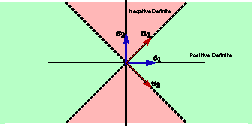
\includegraphics[width=0.95\linewidth]{quadraticformr2.pdf}
        \caption{Diagram showing the regions where $Q$ from example \ref{example:quadraticform} is positive and negative definite, as well as the two lines where it is zero.}
        \label{fig:quadform}
\end{figure}
\begin{remark*}
    In example \ref{example:quadraticform}, we saw that the region where $G$ is positive or negative definite, are not lines through $\RR^2$, and instead they form a kind of flat cone shaped region. Each region consists of infinitely many lines, on which $G$ can be restricted in order to get a positive or negative definite form. In summary, there is no unique subspace $V_0$ of $\RR^2$ where $G|_{V_0}$ is positive definite, and the same can be said for negative definite.
\end{remark*}

\subsubsection{Isometries} 
A nice way to classify bilinear forms is through their set of isometries. Isometries are transformations on $V$ which preserve the bilinear form, and isometry of vector spaces forms an equivalence relation.
\begin{defn}[Pullback of Bilinear Form] \index{Bilinear Form!Pullback}Let $V$ be an $n$ dimensional vector space over a field $\FF$ of characteristic zero. Let $G$ be a nondegenerate symmetric bilinear form on $V$. Let $W$ be some other vector space over $\FF$ and consider a linear map $P : W\to V$. Then we define the \textbf{pullback of $G$ with respect to $P$} to be a bilinear form $P^* G$ on $W$ defined by 
\begin{equation}P^* G(w_1,w_2) = G(P(w_1),P(w_2))\end{equation}
\end{defn}
\begin{defn}[Isometry]\index{Isometry} Let $V_1,V_2$ be two vector spaces, and let $G_1,G_2$ be nondegenerate symmetric bilinear forms on $V_1$ and $V_2$ respectively. Then a map $P : V_1 \to V_2$ is called an \textbf{isometry} if $P^* G_2 = G_1$. 
\end{defn}
\begin{lemma}
    Let $\dim V_1 = \dim V_2$. Then any isometry between $V_1$ and $V_2$ is an isomorphism.
\end{lemma}
\begin{proof}
     Let $v_1\in \ker P$. Then $G_1(v_1,v_2) = G_2(P(v_1),P(v_2))=0$ forall $v_2$. But since $G_1$ is nondegenerate, this is true forall $v_2$ iff $v_1 = 0$. So $v_1=0$ for all $v_1 \in \ker P$. Thus $\ker P = \{0\}$ and so we are done.
\end{proof}
\begin{defn}\index{Isometric}
    Let $V_1,G_1$ and $V_2,G_2$ be vector spaces with nondegenerate symmetric bilinear forms. We say $V_1$ is \textbf{isometric} to $V_2$ if there exists an isometry between them.
\end{defn}
\begin{remark*}
    Isometry is an equivalence relation.
\end{remark*}

\begin{defn}[Orthogonal Group]\index{Group!Orthogonal}\index{Orthogonal!Group} Let $V$ be a vector space and let $G$ be a metric on $V$. The set of all isometries $P : V\to V$ with $P^* G = G$ is a subgroup of $L(V)$ called the \textbf{orthogonal group} and we denote it $\Orth(V,G)$. 
\begin{equation}
    \Orth(V,G) = \{P \in L(V): P^* G= G\}
\end{equation}
\end{defn}
\begin{remark*}
    If $G$ is of signature $(p,q)$ we often write this as $\Orth(p,q,V)$.

    If the vector space is $V=\RR^n$, and $G$ is of signature $(n,0)$ we just write $\Orth(n,\RR)$.
\end{remark*}
\begin{defn}
    \index{Group!Special Orthogonal}
The \textbf{special orthogonal group} $\SO(V,G)$ is the set of all orthogonal transformations $T\in \Orth(V,G)$ with $\det T = 1$.
\end{defn}
\begin{remark*}
An isometry of $V,G$ is sometimes called an orthogonal transformation.
\end{remark*}
\begin{lemma}
    Let $B$ be a basis of $V$. Then $P$ is an isometry of $G$ iff $[P]_B^T[G]_B[P]_B = [G]_B$.
\end{lemma}
\begin{proof}
    Recall that $G(v,w) = [v]_B^T [G]_B[w]_B$. Then \begin{align*}G(P(v),P(w)) &= ([P]_B[v]_B)^T[G]_B[P]_B[w]_B \\&= [v]_B[P]_B^T[G]_B[P]_B[w]_B\end{align*}
    So we need $[P]_B^T[G]_B[P]_B = [G]_B$.
\end{proof}
\subsubsection{Adjoints}
\begin{lemma}
Let $V$ be a finite dimensional vector space over a field $\FF$ of characteristic $0$. Let $G$ be a symmetric or skew nondegenerate bilinear form on $V$. Let $B$ be any other bilinear form on $V$. Then there exists a unique linear map $T_B : V\to V$ so that $B(v,w) = G(T_B(v),w)$ for all $v,w$.
\end{lemma}
\begin{proof}
    Recall the flat map, $\flat_G : V \to V^*$ defined by $\flat_G(v)(w) = G(v,w)$. We know $\flat_G$ is an isomorphism since $G$ is nondegenerate. Let $\flat_B(v)(w) = B(v,w)$ as well. So $B(v,w)=G(T_B(v),w)$ iff $\flat_B(v)(w)=\flat_G(T_B(v))(w)$ for all $w$, if and only if $\flat_B = \flat_G\circ T_B$. So we just have to set $T_B = \flat_G^{-1}\circ \flat_B$. Since $\flat_G$ is an isomorphism and hence invertible, this definition is perfectly good. 
\end{proof}
\begin{remark*}
    So given a fixed nondegnerate bilinear form $G$ on $V$ we have an isomorphism $\iota$ between $V^* \otimes V^*$ and $V\otimes V^*$, given by $\iota(B) = T_B$ as above. 
\end{remark*}
\begin{defn}[Adjoint] Let $G$ be a nondegenerate bilinear form on $V$ (symmetric or skew). For any map $T : V \to V$ we define a linear map $T^\dagger : V \to V$ by the formula $G(v,T(w)) = G(T^\dagger(v),w)$ for all $v,w\in V$. $T^\dagger$ is called the \textbf{adjoint} of $T$.
\end{defn}
\begin{remark*}
    $T^\dagger$ is not the same as the dual map $T^*$. But they are related by a formula.
\end{remark*}
\begin{lemma}
    The map $T^\dagger$ is the only map satisfying $G(v,T(w))=G(T^\dagger(v),w)$ for all $v,w$.
\end{lemma}
\begin{proof}
    Let $B \in V^*\otimes V^*$ where $B(v,w)=G(v,Tw)$. Then there is a unique map $T_B : V\to V$ given by $B(v,w) = G(T_B(v),w)$. Therefore we have $G(T_B(v),w)=G(v,T(W))$ so $T_B = T^\dagger$ as required.
\end{proof}
\begin{remark*}
    Since $G$ is either skew or symmetric, $
G(v,Tw) = G(T^\dagger v,w)$ implies that $\pm G(T(w),v) = \pm G(w,T^\dagger V)$. So $G(T(v),w) = G(v,T^\dagger(w))$. Therefore $T$ satisfies the same definition as $(T^\dagger)^\dagger$. Since adjoints are unique, $T = (T^\dagger)^\dagger$.

It also follows that $(T\circ S)^\dagger = S^\dagger\circ T^\dagger$.
\end{remark*}
\begin{remark*}
    The dual map and the adjoint are related. Observe, $G(v,T(w)) = G(T^\dagger (v),w)$, so $\flat_G(v)(T(w)) = \flat_G(T^\dagger(v))(w)$. But $\flat_G(v)(T(w)) = T^*\flat_G(v)(w)$, so $T^*(\flat_G) = \flat_G \circ T^\dagger$. Hence,
    \begin{equation}
        T^\dagger = \flat_G^{-1} \circ T^*(\flat_G) = \sharp_G\circ T^*\circ \flat_G
    \end{equation}
\end{remark*}

\begin{defn}[Self/Skew-Adjoint]\index{Operator!Self-Adjoint}\index{Operator!Skew-Adjoint} A map $T : V \to V$ is called self-adjoint if $T^\dagger = T$. It is called skew-adjoint if $T=-T^\dagger$.
\end{defn}
\begin{remark*}
    Let $T \in L(V)$. Then we can write $T = \frac{1}{2}(T+T^\dagger)+\frac{1}{2}(T-T^\dagger)$. Observe that $\frac{1}{2}(T+T^\dagger)$ is self adjoint and $\frac{1}{2}(T-T^\dagger)$ is skew-adjoint!
\end{remark*}
\begin{lemma}
    $B$ is symmetric iff $T_B$ is self-adjoint, and $B$ is skew iff $T_B$is skew-adjoint.
\end{lemma}
\begin{proof}
    Let $B \in V^*\otimes V^*$ and let $T_B \in \End(V)$. We have $B(v,w) = G(T_B(v),w) = G(v,T_B^\dagger(w)) = \pm G(T^\dagger(w),v)$. Suppose $G$ is symmetric. Then $B(v,w) = G(T^\dagger_B(w),v) = G(T_B(w),v)$ for all $v,w$. Since $G$ is nondegenerate, we have $T^\dagger_B(w)=T_B(w)$ for all $w$. This means $T_B$ is self adjoint. 

    For the other direction, we see that if $T_B$ is self adjoint then $B(v,w) = G(T_B(v),w) = G(w,T_B(v)) = B(w,v)$. 

    If we did this proof again for skew $G$, then we would have a minus sign everywhere. Therefore the proof for skew-adjoint $T_B$ is identical.
\end{proof}

\subsection{Lecture 7: Reflections, Hyperbolic Planes, and Cancellation}

\subsubsection{Adjoint Basis}
For all of this lecture, $V$ is a finite dimensional vector space over a field $\FF$ of characteristic zero, and $G$ is a symmetric bilinear form.

Recall that $\flat : V \to V^*$ and $\flat(v)(w) = G(v,w)$. Let $B = \{e_1,...,e_n\}$ and $B^* = \{e^1,...,e^n\}$.
Let $\flat(e_i) = A_{ij} e^j$. Observe that $\flat(e_i)(e_j) = G_{ij} = A_{ij}$. So $[\flat]_{B^* B} = [G]_B$.
\begin{defn}[$G$-adjoint Basis]\index{Basis!G-adjoint}The set $\{\flat(e_i) : i =1,...,n\}$ is a basis for $V^*$ called the $G$-adjoint basis. We denote it by $B^\dagger$.\end{defn}
\begin{remark*}
    If $B$ is an orthonormal basis then $B^* = B^\dagger$. In this basis $[T]^\dagger_B = [T]^T_B$.
\end{remark*}

\subsubsection{Classification of Bilinear Forms: Symmetric Bilinear Forms Part 3}
The problem is to classify all symmetric nondegenerate bilinear forms (metrics) on $V$. Given a vector space $V$, can we classify all possible metrics up to isometry (that is, we only say two metrics are different if we can not transform one into another via an isometry). This classification will be based off the proof in the book Basic Algebra I by Jacobson \cite{Jacobson2009-pp}.

\begin{defn}[Reflection]\index{Reflection} Let $v$ be a vector which is not isotropic, so $Q(v)\neq 0$. Then we define a linear map $R_v : V \to V$ by $R_v(u) = u-2\frac{G(u,v)}{Q(v)}v$. This map is called a \textbf{reflection generated by $v$}
\end{defn}
\begin{remark*}
    $R_{tv} = R_v$ for all $t\in\RR$
\end{remark*}
\begin{lemma}
 The map $R_v$ is an isometry.   
\end{lemma}
\begin{proof}
    By the polarization identity, the map $R_v$ is an isometry iff $Q(R_v(u))=Q(u)$ for all $u\in V$. We have
    \begin{align*}
        Q(R_v(u))&=Q\left(u-2\frac{G(u,v)}{Q(v)}v\right)\\
        &= G\left(u-2\frac{G(u,v)}{Q(v)}v,u-2\frac{G(u,v)}{Q(v)}v\right)\\
        &= Q(u) - 4\frac{G(u,v)G(v,u)}{Q(v)}+4\frac{G(u,v)^2G(v,v)}{Q(v)}\\
        &= Q(u)
    \end{align*}
    Where we have used the fact that $G$ is symmetric to cancel out the last two terms. 
\end{proof}

\begin{remark*}
    Let $u \in \Span\{v\}^\perp$. Then $G(u,v)=0$, so $R_v(u)=u$.
\end{remark*}
\begin{remark*}
    Suppose $u=v$. Then $R_v(u) = v-2v = -v$.
\end{remark*}
\begin{remark*}
    Based on the above two facts, we observe that $R_v$ is a reflection over the hyperplane $\Span\{v\}^\perp$.
\end{remark*}
\begin{example}
    Let $V = \RR^3$ and let $G$ be the standard inner product, $G(v,w) = v^1 w^1 + v^2 w^2 + v^3 w^3$. We have the following picture. 
\end{example}
\begin{figure}[h!]
    \centering
    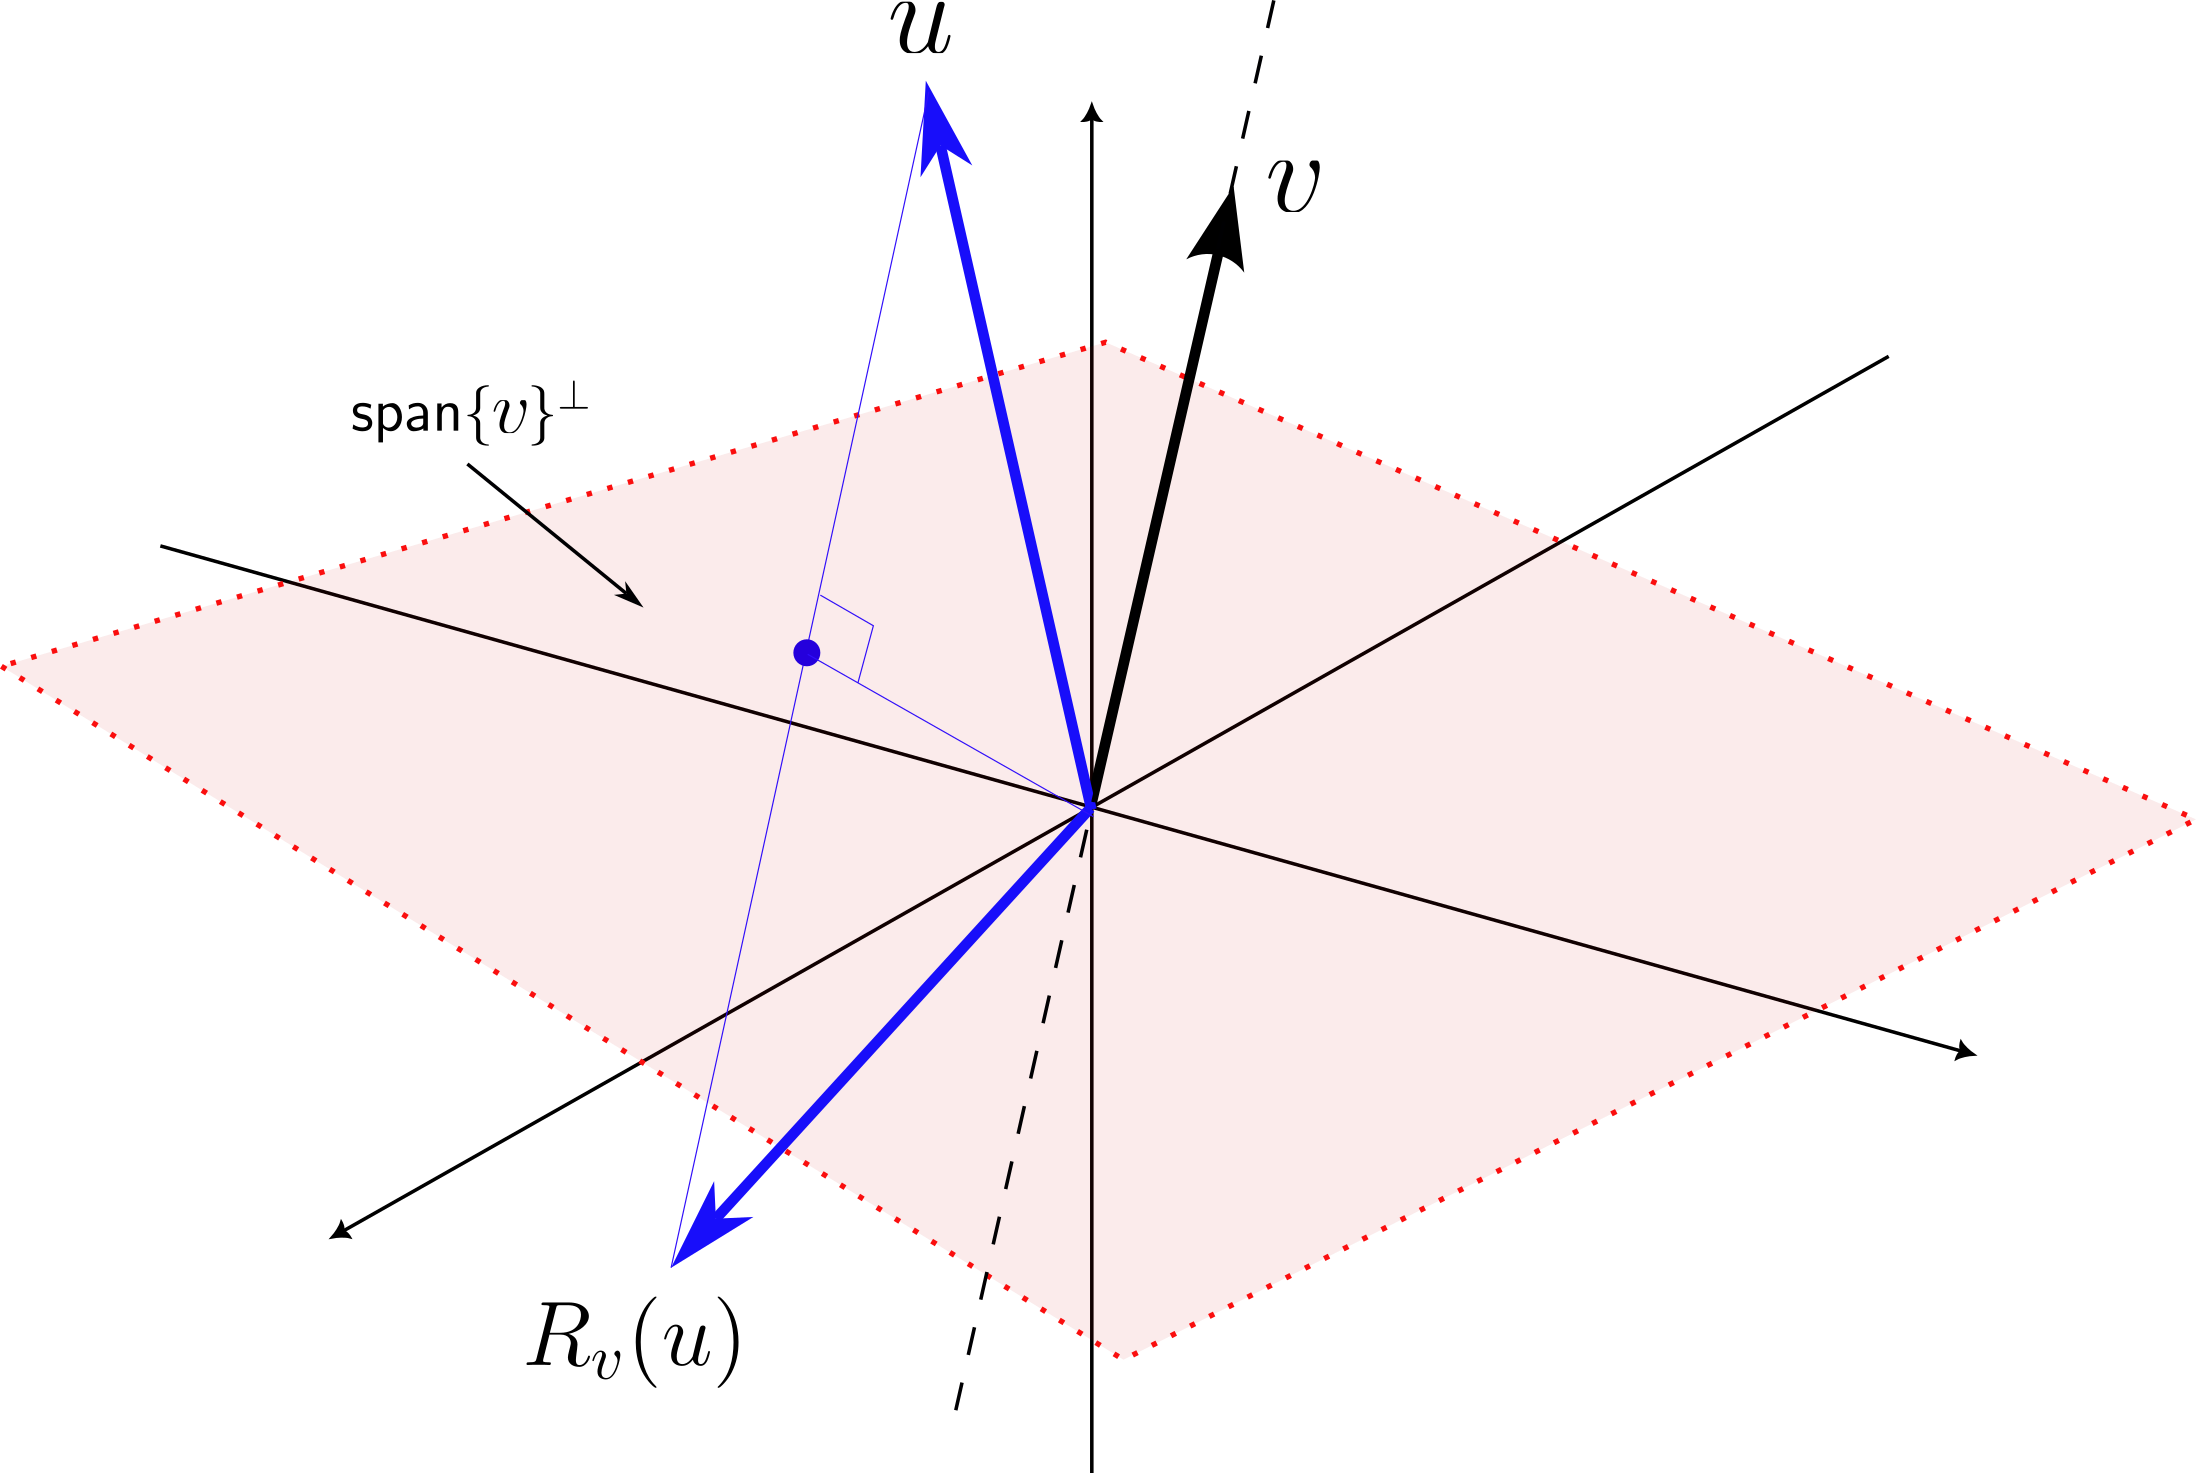
\includegraphics[width=0.6\linewidth]{reflection.png}
    \caption{Diagram of a reflection in $\RR^3$ using the standard inner product.}
    \label{fig:reflectionr3}
\end{figure}
\begin{remark*}
    Let $e_1=v$ and let $e_2,...,e_n$ be a basis for $\Span\{e_1\}^\perp$. Then $B = \{e_1,...,e_n\}$ is a basis for $V$ and $[R]_B = \diag(-1,1,...,1)$. So $\det R_v = -1$. 
\end{remark*}
\begin{defn}
    Let $T : V \to V$ be an isometry. Recall that since $T$ is an isomorphism, $\det T \neq 0$. We say that $T$ is \textbf{proper} if $\det T >0$ and \textbf{improper} if $\det T<0$. \index{Isometry!Proper/Improper}
\end{defn}
\begin{remark*}
    Reflections are improper isometries.
\end{remark*}
\begin{lemma}
    Let $P$ be an isometry. Then $P R_v P^{-1}$ is a reflection, and in fact $P R_v P^{-1} = R_{Pv}$.
\end{lemma}
\begin{proof}
    \begin{align*}
        P R_v P^{-1}(u) &= P(P^{-1}(u) - \frac{2G(P^{-1}(u),v)v}{Q(v)})\\
        &= u-\frac{2 G(P^{-1}(u),P^{-1}(P(v))}{Q(P(v))}P(v)\\
        &= u-\frac{2 G(u,P(v)}{Q(P(v))}P(v)\\
        &= R_{P(v)}(u)
    \end{align*}
    Where we have used the fact that $P$ is an isometry to say $Q(P(v))=Q(v)$ and $G(P^{-1}(x),P^{-1}(y))=G(x,y)$.
\end{proof}
\begin{defn}[$T$-invariant Subspace] Let $T:V\to V$ be linear and let $U$ be a subspace of $V$. We say $U$ is $T$-invariant if $T(U) \subseteq U$.
\end{defn}
\begin{lemma}
    Let $U$ be a $T$-invariant subspace. Then $U^\perp$ is a $T^\dagger$-invariant subspace.
\end{lemma}
\begin{proof}
    Let $v \in U^\perp$. This means that $G(u,v) = 0$ for all $u \in U$. Therefore $G(u,T^\dagger(v))=G(T(u),v) = 0$ for all $v$ since, because $U$ is $T$-invariant, we know $T(u)\in U$. In other words, we have $G(u,T^\dagger(v))=0$ for all $u\in U$, which means by definition that $T^\dagger(v) \in U^\perp$.
\end{proof}
\begin{cor}
Let $T \in \Orth(V,G)$. If $T(U)\subseteq U$, then $T(U^\perp) = U^\perp$.
\end{cor}
\begin{proof}
    We know $T(U)\subseteq U$. Since $T$ is injective, $\dim T(U) = \dim U$. Therefore $T(U)=U$ and $U=T^{-1}(U)$. Therefore $T^\dagger(U)=U$. Applying the lemma, we have $(T^\dagger)^\dagger (U^\perp) \subseteq U^\perp$, so $T(U^\perp)\subseteq U^\perp$, and because $T$ is injective, we furthermore have $T(U^\perp) = U^\perp$.
\end{proof}
\begin{remark*}
    Note that we have not said anything about whether $G|_U$ is nondegenerate or not.
\end{remark*}
\begin{defn}
    We say $V$ is an \textbf{orthogonal direct sum} of the subspaces $U_1,...,U_k\subseteq V$ if $V = \bigoplus_{i=1}^k U_i$ and $U_i\perp U_j$ for all $i\neq j$. Notationally we write $V = U_1 \orthoplus U_2 \orthoplus...\orthoplus U_k = \bigorthoplus_{i=1}^k U_i$.
\end{defn}
\begin{remark*}
    The above definition is about decomposing a vector space into a direct sum of smaller, mutually orthogonal vector spaces. 
\end{remark*}
\begin{remark*}
    Notice that for each $j$, we have $U_j^\perp = \bigoplus_{i=1, i\neq j}^k U_i$.
\end{remark*}
\begin{remark*}
    Suppose that $V = \bigorthoplus_{i=1}^k U_i$, which means that any vector $v$ can be written as $v=\sum_{i=1}^k u_i$, where $G(u_i,u_j) = 0$ if $i\neq j$. Then $Q(v) = \sum_{i=1}^k Q(u_i)$.
\end{remark*}
\begin{lemma}
    Suppose that $V = \bigorthoplus_{i=1}^k \tilde{U}_i$, and $V = \bigorthoplus_{i=1}^k U_i$, and let $v = \sum_{i=1}^k u_i$ and $v = \sum_{i=1}^k\tilde{u}_i$. Suppose for each $i=1,...,k$ we have an isometry $P_i : U_i \to \tilde{U}_i$. Define $P : V \to V$ by $P(\sum_{i=1}^k u_i) = \sum_{i=1}^k P_i u_i$. Then $P$ is an isometry.\label{lemma74}
\end{lemma}
\begin{remark*}
     \begin{align*}Q(P(v)) &= Q(\sum_{i=1}^k P_i(v_i)) \\&= \sum_{i=1}^k Q(P_i(v_i)) \\&= \sum_{i=1}^k Q(v_i) \\&= Q(v)\end{align*}
\end{remark*}
So we can build isometries of $V$ out of isometries on the orthogonal components of $V$.
\subsubsection{Hyperbolic Planes}
We will take a detour here to talk about hyperbolic planes.
\begin{defn}
    Let $U$ be a vector subspace of $V$. Then $U$ is said to be isotropic if $Q|_U=0$, or equivalently $U \subseteq U^\perp$.\index{Isotropic!Subspace}
\end{defn}
\begin{remark*}
    An isotropic vector generates an isotropic vector subspace. That is, if $v$ is isotropic then $\Span\{v\}$ is an isotropic subspace.
\end{remark*}
If $\FF = \RR$ and $G$ is positive definite or negative definite then there are no isotropic subspaces.
\begin{defn}\index{Hyperbolic Plane}
    Let $G$ be a metric on $V$. We say that $V$ is a \textbf{hyperbolic plane} if $\dim V = 2$ and $V$ contains an isotropic vector.
\end{defn}
\begin{thm}
    Let $\dim V = 2$, and let $G$ be a metric. The following are equivalent.
    \begin{enumerate}[i)]
    \item {
    $V$ is a hyperbolic plane.
    }
    \item {
    There exists a basis $B=\{u,v\}$ of $V$ so that $Q(u)=0$, $Q(v)=0$, and $G(u,v)=G(v,u)=1$. That is,
    \[[G]_B = \m{0&1\\1&0}\]
    Such a basis is called a \textbf{hyperbolic basis}\index{Basis!Hyperbolic}
    }
    \item {
    For all bases $B$ of $V$, $\det [G]_B = -x^2$ for some $x \in \FF$.
    }
    \end{enumerate}
\end{thm}
\begin{proof}
    First we show that i implies ii. First, there exists $u$ so that $Q(u)=0$. Then by nondegeneracy there is some $v$ so that $G(u,v)\neq 0$. Then since $G(u,u)=0$, $v\neq u$, so $\{u,v\}$ is a linearly independent set and hence a basis. Without loss of generality we may set $G(u,v)=1$ by rescaling $v$. Then let $a \in \FF$, and set $\tilde{v} = v+au$. Then $Q(\tilde{v}) = Q(v)+2a$. Choose $a = -\frac{1}{2}Q(v)$. So $Q(\tilde{v})=0$ and $\{u,\tilde{v}\}$ is linearly independent, and therefore is a basis satisfying the requirements of ii.

    Now we show that ii implies iii. Let $B$ be the aforementioned basis. Then 
    \[[G]_B = \m{0&1\\1&0}\]
    which has determinant $-1$ as required. If $\tilde{B}$ is another basis then $[G]_{\tilde{B}} = -\det(P_{B\tilde{B}})^2$ which is of the form $-x^2$ as required.

    Finally we show that iii implies i. Suppose $\det [G]_B = -x^2,x\neq0$ for all bases $B$. This means $G$ is nondegenerate, and furthermore there exists a basis $B=\{e_1,e_2\}$ so that $[G]_B = \diag(b_1,b_2)$. This means $b_1b_2 = -x^2$ for some $x$. Now let $w = c_1 e_1 + c_2 e_2$. Then \[Q(w) = c_1^2 b_1 + c_2^2 b_2\]
    Then let $c_1 = a$ and $c_2 = b_2$, so then 
    \[Q(w) = a^2 b_1 + b_1^2 b_2 = b_1(a^2+b_1b_2)=b_1(a^2-a^2)=0\]
    So $w$ is an isotropic vector, which is what we needed to find. This completes the proof.
\end{proof}
\begin{cor}
    Any two hyperbolic planes are isometric.
\end{cor}
\begin{proof}
    Let $V,G$ and $\tilde{V},\tilde{G}$ be two hyperbolic planes. Then there are bases $B=\{e_1,e_2\},\tilde{B}=\{\tilde{e}_1,\tilde{e}_2\}$ so that \[[G]_B = [\tilde{G}]_{\tilde{B}} = \m{0&1\\1&0}\]
    Let $P : V\to \tilde{V}$ so that $P(e_1)=\tilde{e}_1,P(e_2)=\tilde{e}_2$, and extend the definition by linearity. Then $P^T [G]_B P = [G]_{\tilde{B}}$ which means $P$ is an isometry as required.
\end{proof}
\begin{thm}
    Any hyperbolic plane $V$ contains exactly two one-dimensional isotropic subspaces.
\end{thm}
\begin{proof}
    Let $\{u,v\}=B$ be a hyperbolic basis for $V$. Then let $w \in V$. Then $w = au+bv$ and $Q(w)=2ab$. This is zero iff $a=0$ or $b=0$. Therefore $w=au$ or $w=bv$. Thus $w$ is isotropic iff $w \in \Span\{u\}$ or $w\in \Span\{v\}$. These are the two isotropic subspaces.
\end{proof}
\begin{remark*}
    The figure presented earlier, figure \ref{fig:quadform}, shows the isotropic subspaces for the choice of metric,
    \[[G]_S = \m{0&1\\1&0}\]
    Any hyperbolic plane metric can be put in this form, if we use the basis $e_1 = \frac{u+v}{4G(u,v)}$ and $e_2 = \frac{u-v}{4G(u,v)}$. Therefore, figure \ref{fig:quadform} provides a decent visual of what the isotropic subspaces look like. In general, we get the same picture but warped by some shear/rotation.
\end{remark*}
\begin{defn}
    Let $\FF$ be a field. The \textbf{group of units} of $\FF$ is the set of all invertible elements of $\FF$. That is, 
    \begin{equation}\FF^* = \{a \in \FF: \exists b \in \FF, ba=ab=1\}.\end{equation}\index{Group!of Units}
\end{defn}
\begin{thm}
    Let $V,G$ be a hyperbolic plane. Then,
    \begin{enumerate}[a)]
    \item {
    Any improper isometry is a reflection.
    }
    \item {
    The special orthogonal group of $G$ is isomorphic to the group of units of $\FF$. That is, $\SO(V,G) = \FF^*$
    }
    \end{enumerate}
\end{thm}
\begin{proof}
    Let $P\in \Orth(V,G)$ be any orthogonal transformation and let $\{u,v\}$ be a hyperbolic basis. Then $P$ maps isotropic subspaces to isotropic subspaces since $Q(P(v))=Q(v)$. So either $P$ takes $\Span\{u\}$ to $\Span\{u\}$ and $\Span\{v\}$ to $\Span\{v\}$ or it exchanges them. In the first case, $P(u) = au$ and $P(v) = bv$ for some $a,b\in\FF$. Therefore $[P]_B = \diag(a,b)$. So $1=G(u,v)=G(P(u),P(v)) = G(u,v)ab=ab$. Therefore $b=a^{-1}$, meaning $[P]_B = \diag(a,a^{-1})$ and $\det [P]_B = 1$. So $P\in \SO(V,G)$. Therefore every isometry which leaves the two isotropic vector spaces where they are is an element of $\SO(V,G)$.

    In the other case, we have $P(u)=av$ and $P(v)=bu$. So $G(u,v)=ab$, and \[[P]_B = \m{0&a^{-1}\\a&0}\]
    so $\det [P]_B = -1$. This is not an element of $\SO(V,G)$, but it is a reflection. Observe that $P(u+av) = av+a a^{-1}u = u+av$ and $P(u-av) = av-u = -(u-av)$. Since $G(u+av,u-av) = 0+a-a+0=0$, we finally have $P = R_{u-av}$. This proves part a).

    The previous two points imply that $\SO(V,G)$ consists entirely of isometries which leave the two isotropic subspaces where they are.

    Finally, let $\varphi : \SO(V,G) \to \FF^*$ be defined by $\varphi(P) = \varphi(\diag(a,a^{-1})) = a$. This is well defined because we just showed that the only elements of $\SO(V,G)$ are those which can be put in the form $\diag(a,a^{-1})$. This is a group isomorphism since $\varphi^{-1}(a) = \diag(a,a^{-1})$ is defined and 
    \begin{align*}\varphi(AB) &= \varphi(\diag(a,a^{-1})\diag(b,b^{-1})) \\&= \varphi(\diag(ab,(ab)^{-1})) = ab \\&= \varphi(A)\varphi(B)\end{align*}
\end{proof}

\subsubsection{Witt's Cancellation Theorem}
\begin{defn}
   Let $U$ be a subspace of $V$, and let $G$ be nondegenerate. If $G|_U$ is nondegenerate we say $U$ is a \textbf{nondegenerate subspace}.\index{Subspace!Nondegenerate}
\end{defn}
\begin{thm}[Witt Cancellation Theorem]\index{Theorem!Witt Cancellation Theorem}\index{Witt!Cancellation Theorem}
Let $V,G$ be a vector space over a field $\FF$ of characteristic zero where $G$ is a metric. Suppose $U_1,U_2$ are nondegenerate subspaces of $V$. If $U_1$ is isometric to $U_2$ then $U_1^\perp$ is isometric to $U_2^\perp$.\label{thm:wittcancel}
\end{thm}
\begin{proof}
    If $U_1,U_2$ are nondegenerate subspaces then $V = U_1\orthoplus U_1^\perp$ and $V=U_2\orthoplus U_2^\perp$. So what we are trying to show is that if $U_1$ and $U_2$ are isometric, we can ``cancel" them on both sides of the equation $U_1\orthoplus U_1^\perp = U_2\oplus U_2^\perp$.

    First observe that $G|_{U_1}$ and $G|_{U_2}$ are both nondegenerate.

    Now, let $U_1$ and $U_2$ be isometric. Then first of all, $\dim U_1 = \dim U_2 = k$. We will prove this by using mathematical induction on $k$. Let us begin with $k=1$ as the base case.

    In the base case, $U_1 = \Span\{u_1\}$, $U_2=\Span\{u_2\}$, and $Q(u_1)\neq 0, Q(u_2)\neq 0$. By scaling $u_2$ appropriately, let $Q(u_1)=Q(u_2)$. Then \[Q(u_1\pm u_2) = Q(u_1)\pm 2G(u_1,u_2)+Q(u_2) = 2Q(u_1)\pm 2G(u_1,u_2)\]
    
    We claim that either $Q(u_1+u_2)\neq 0$ or $Q(u_1-u_2)\neq 0$ (but not both!)

    If they are both zero, then we could expand then add them together and get $Q(u_1)=Q(u_2)=0$.

    If we know that $Q(u_1+u_2)\neq 0$, then we also know that $G(u_1+u_2,u_1-u_2) = Q(u_1)-Q(u_2)=0$, so $u_1+u_2\perp u_1-u_2$. Furthermore, $R_{u_1+u_2} (u_1-u_2)=u_1-u_2$, and so \[R_{u_1+u_2}(u_1-u_2)+R_{u_1+u_2}(u_1+u_2) = R_{u_1+u_2}(2u_1) = -2u_2\] This means that $R_{u_1+u_2}$ takes $\Span\{u_1\}$ to $\Span\{u_2\}$ and vice versa, and also that $R_{u_1+u_2}$ takes $\Span \{u_1\}^\perp$ to $\Span\{u_2\}^\perp$. Therefore $R_{u_1+u_2}$ is an isometry between $U_1^\perp$ and $U_2^\perp$ as required.

    Now suppose instead that we know $Q(u_1-u_2)\neq 0$. Then we could take $R_{u_1-u_2}$ and find $R_{u_1-u_2}(u_1)=u_2$, and then get the same result. This finishes the base case.

    See Jacobson chapter 6 for the inductive step \cite{Jacobson2009-pp}. 
\end{proof}
\begin{remark*}
    Witt's Cancellation theorem, along with lemma \ref{lemma74} hints at the fact that if we have an isometry between nondegenerate subspaces $U_1$ and $U_2$, then we can extend it to an isometry from $V$ to $V$. This will be proven at the beginning of next lecture.
\end{remark*}
\subsection{Lecture 8: Witt Extension Theorem, Maximally Isotropic Subspaces, and the Cartan-Dieudonn\'e Theorem}
\subsubsection{Witt Extension Theorem}
\begin{lemma}
    Let $V,G$ be a vector space with metric, and let $U\subseteq V$ be a degenerate subspace. That is, a subspace with $\Radical (G|_U) \neq \{0\}$. Let $U'$ be any subspace with the property that $V=U' \oplus \Radical(G|_U)$. Let $r = \dim \Radical(G|_U)$. Then there exist hyperbolic planes $H_1,...,H_r$ and a subspace $W \subseteq V$ so that $U\oplus W = U'\orthoplus H_1\orthoplus ...\orthoplus H_r$.
\end{lemma}
\begin{remark*}
    This lemma says that if we have a degenerate subspace $U$, there is always some other subspace $W$ we can add it to and get a nondegenerate subspace. Furthermore, the sum of these two subspaces decomposes into a nice nondegenerate space $U'$ along with a bunch of hyperbolic planes $H_i$, which are easy to work with.
\end{remark*}
\begin{proof}
    Let $\{u_1,...,u_r\}$ be a basis of $\Radical(G|_U)$. Let $\alpha \in U^*$ be defined so that $\alpha(u_1)=1$ and $\alpha(u_i)=0$ for $i=2,...,r$ and $\alpha(U')=0$. 
    
    Then since $G$ is nondegenerate on $V$ there exists some $v_1 \in V$ so that $\alpha(u)=G(u,v_1)$ for all $u$. So, there is some $v_1$ with $G(u_1,v_1)=1$, $G(u_i,v_1)=0$ for $i=2,...,r$, and $G(u,v_1)=0$ for all $u\in U'$. 
    
    Note that $v_1$ is not an element of $U$. Then replace $v$ by $\tilde{v}_1 = v_1+\sigma u_1$, for some $\sigma \in \FF$. 
    
    Then $Q(\tilde{v}_1) = Q(v_1)+2\sigma$. So we set $\sigma = -Q(v_1)/2$, to get $\{u_1,\tilde{v}_1\}$ to span a hyperbolic plane. So we set 
    $H_1 = \Span\{u_1,\tilde{v}_1\}$.
    
    Furthermore, by definition of $\perp$ we have $V = H_1\orthoplus H_1^\perp$. Now let $\tilde{U} = U' \oplus \Span\{u_2,...,u_r\}\subseteq \Span\{u_1,v_1\}^\perp$.
    
    Note that $\Radical(G|_{\tilde{U}}) = \Span\{u_2,...,u_r\}$. If $r=1$ we have $U' = \tilde{U}$ and we can let $W = \Span\{v_1\}$ so that $U\oplus W = U' \oplus H_1$. 
    
    Otherwise, set $U,V = \tilde{U},\tilde{V}$ in the above argument and repeat. Inductively, we will get $r$ hyperbolic planes $H_1,...,H_r$ until finally we have $U\oplus W = U' \orthoplus H_1\orthoplus...\orthoplus H_r$ as required. We also verify that $U\oplus W$ is nondegenerate, since everything in the big orthogonal direct sum is.  
\end{proof}
\begin{remark*}
    This proof is quite inscrutable. The idea is that, since $U$ is degenerate, we can find an isotropic vector $u_1$ in $U$. This vector gives us the first basis vector for the hyperbolic plane. Then we find another vector, $\tilde{v}_1$ which is also isotropic, and the span of the two isotropic vectors gives us the first hyperbolic plane $H_1$. Then, we check whether the complement of $H_1$ in $U$ is degenerate. If not, we are done and $W$ is just the span of $v_1$. Otherwise, since the complement is degenerate we can find another isotropic vector and repeat the process.

    The main idea is to find all of the linearly independent isotropic vectors in $U$, and pair each of them up with an isotropic vector in the larger space $V$ so that their span is non degenerate. To do this, we have to make $U$ into a bigger subspace, which is $U\oplus W$.
\end{remark*}

\begin{thm}[Witt Extension Theorem] Let $U_1$, $U_2$ be subspaces of $V$ and let $P : U_1\to U_2$ be an isometry. Then there exists an isometry $P:V\to V$ so that $P|_{U_1} = \tilde{P}$.\index{Theorem!Witt Extension Theorem}\index{Witt!Extension Theorem}
\end{thm}

\begin{proof}
    If $U_1$ is nondegenerate, this is a direct consequence of Theorem \ref{thm:wittcancel} and Lemma \ref{lemma74}.

    If $U_1$ is degenerate, then there exists some $W_1$ so that $U_1\oplus W_1 = U_1' \orthoplus H_1\orthoplus...\orthoplus H_r$, where $U_1'$ has the property that $U_1 = \Radical(G|_{U_1})\oplus U_1'$. Let $\tilde{P} = P|_{U_1}$. Then $\tilde{P}$ maps $U_1$ to $U_2$, and $\tilde{P}|_{\Radical(G|_{U_1})}$ is an isomorphism between $\Radical(G|_{U_1})$ and $\Radical(G|_{U_2})$. We then set $U_2' = P(U_1')$m which means there exists $W_2$ so that $U_2\oplus W_2 = P(U_1')\orthoplus H_1\orthoplus...\orthoplus H_r = U_2' \orthoplus\tilde{H}_1\orthoplus...\orthoplus \tilde{H}_r$. Here, $H_i = \Span\{v_i,u_i\}$ and $\tilde{H}_i = \Span\{\tilde{v}_i,P(u_i)\}$.

    Now we define $L : U_1\oplus W_1 \to U_2 \oplus W_2$ by $L|_{U_1} = P$ and $L|_{W_1}(v_i) = \tilde{v}_i$ for $i=1,...,r$. Since $v_i \in W_1$, $\tilde{v}_i\in W_2$, and $U_1\oplus W_1$ is nondegenerate, this is an isometry by construction. Since $U_1\oplus W_1$ is nondegenerate, we then see that by Theorem \ref{thm:wittcancel} and Lemma \ref{lemma74}, $L$ can be extended to all of $V$. Since $L$ is in turn an extension of $P$, we are done.
\end{proof}
\begin{remark*}
    A useful application of this theorem is the Witt index.
\end{remark*}
\subsubsection{Maximally Isotropic Subspaces}
\begin{remark*}
    Recall that $U_1$ is an isotropic subspace if $G|_{U_1} = 0$. If $U_2$ is another isotropic with $\dim U_1 = \dim U_2$ then any isomorphism between $U_1$ and $U_2$ is an isometry, and can be extended to $V$ to get an isometry.
\end{remark*}
\begin{defn}[Maximally Isotropic Subspace]\index{Subspace!Maximally Isotropic}
An isotrophic subspace $U\subseteq V$ is said to be \textbf{maximal} if whenever we have another isotropic space $W$ with $U\subseteq W\subseteq V$, then $U=W$.
\end{defn}
\begin{lemma}
    If $U$ is maximally isotropic and $\tilde{U}$ is isotropic then there is an isometry $P : V \to V$ with $P(\tilde{U})\subseteq U$.
\end{lemma}
\begin{proof}
    Suppose $\dim \tilde{U} < \dim U$. Then there is a subspace of $U$ of dimension $\dim \tilde{U}$, and therefore an isomorphism between $\tilde{U}$ and a subspace of $U$. Since any isomorphism between isotropic subspaces is an isometry, this case is done.

    If $\dim \tilde{U} \geq \dim U$, then there is an isometry $P$ with $P(U)\subseteq \tilde{U}$, which means $P^{-1}(\tilde{U})$ is isotropic. This means $U \subseteq P^{-1}(\tilde{U})\subseteq V$. Since $U$ is maximal, $P^{-1}(\tilde{U}) = U$, so $\tilde{U} = P(U)$. This completes the proof for all possible cases.
\end{proof}

\begin{cor}
    All maximally isotropic subspaces of $V$ are the same dimension.
\end{cor}
\begin{proof}
    If $U$ and $\tilde{U}$ are maximally isotropic, then $\dim U \leq \dim \tilde{U}$ by the previous lemma, and vice versa, so $\dim U = \dim \tilde{U}$.
\end{proof}
\begin{defn}[Witt Index]\index{Witt!Index}
    Let $U$ be a maximally isotropic subspace. Then we define $\nu(V) = \dim U$ to be the \textbf{Witt index} of $V$. Notice that it does not depend on the choice of maximally isotropic subspace.
\end{defn}

\begin{lemma}
    Let $\dim V = n$. Then $\nu(V) \leq \floor{\frac{n}{2}}$.\label{lemma83}
\end{lemma}
\begin{proof}
    Let $U$ be a maximally isotropic subspace of $V$. Then $U$ can be extended into $U\oplus W = \bigoplus_{i=1}^r{}_\perp H_i$, where $U' = \{0\}$ since $U$ is maximally isotropic. Since $\dim H_i = 2$, we have $\dim U\oplus W = \nu(V) + \dim W = 2r\leq  n$. So $r \leq \frac{n}{2}$. Since $r$ is an integer, we furthermore have $r\leq \floor{\frac{n}{2}}$. Since $U$ is isotropic, $\Radical (G|_{U}) = U$, so $r=\dim U$. This completes the proof.
\end{proof}
\begin{defn}[Anisotropic Kernel]
    Let $U$ be maximally isotropic. Then there is some $W$ so that $U\oplus W$ is nondegenerate and $V = (U\oplus W)\orthoplus(U\oplus W)^\perp$, where $(U\oplus W)^\perp$ is anisotropic. The space $(U\oplus W)^\perp$ is called an \textbf{anisotropic kernel} of $G$.
\end{defn}
\begin{remark*}
    Let $\mu \leq \nu$. Suppose we had the following decompositions of $V$, where $X$ and $\tilde{X}$ are anisotropic subspaces,
    \[V = H_1\orthoplus...\orthoplus H_\nu \oplus X\]
    \[V = \tilde{H}_1\orthoplus...\orthoplus \tilde{H}_\nu \oplus \tilde{X}\]
    Let $\{\tilde{u}_i,\tilde{v}_i\}$ be a hyperbolic basis for $\tilde{H}_i$ for each $i=1,...,\nu$. Then $\Span\{\tilde{u}_1,...,\tilde{u}_\mu\}$ is isotropic, and $\mu \leq \nu$, so there is an isometry between $H_1\orthoplus...\orthoplus H_\mu$ and $\tilde{H}_1\orthoplus...\orthoplus \tilde{H}_\mu$. By the extension theorem we can extend this to an isometry $H_{\mu+1}\orthoplus...\orthoplus H_\nu \orthoplus X \to\tilde{X}$. But $\tilde{X}$ is anisotropic, so $\mu=\nu$ and $\tilde{X}=X$. So the study of metrics reduces up to isometry to the study of anisotropic metric vector spaces. For general $\FF$ this becomes complicated.
\end{remark*}
    \subsubsection{Classification of Bilinear Forms: Symmetric Bilinear Forms Part 4, Cartan-Dieudonn\'e theorem}
    \begin{thm}[Cartan-Dieudonn\'e Theorem]
    Let $\FF$ be a field of characteristic not equal to $2$. Let $G$ be a metric on $V$, and let $\dim V = n$. Let $P$ be an isometry of $V$. Then $P$ is the product of $k\leq n$ reflections.\index{Theorem!Cartan-Dieudonn\'e Theorem}\end{thm}
    \begin{proof}
        We prove this by induction on $n$.
        
        First suppose $n=1$ for the base case.
        Let $\{v\}$ be a basis of $V$. Then $Pv =\lambda v$ for some $\lambda$, so $Q(P(v))=\lambda^2 Q(v)$. So $\lambda = \pm 11$. In the positive case $P=\One$ and in the negative case $P = R_{-v}$. So $P$ is either a product of zero or one reflections as required.

    The inductive step splits into three cases.
    \begin{enumerate}
    \item {
    Let $V_1 = \{v\in V :Pv = v\}$. Suppose $V_1$ is anisotropic. Then there exists $u\neq 0$ so that $Q(u)\neq 0$ and $P(u) = u$. So $P$ maps $\Span\{u\}^\perp$ to $\Span\{u\}^\perp$, and so $P|_{\Span\{u\}} = \One$, so $P = \One_{1\times 1} \oplus P|_{\Span\{u\}^\perp}$. So the problem reduces to $\Span\{u\}^\perp$ which is $n-1$ dimensional. If it is anisotropic, we repeat the procedure. Otherwise we go to another one of the cases, and try to show that $P|_{\Span\{v\}^\perp}$ and hence $P$ is the product of at most $n-1$ reflections.
    }
    \item {
    Suppose there exists $u\neq 0$ so that $Q(v)\neq 0$ and $Q(v-P(v))\neq 0$. Since $P$ is an isometry, $Q(P(v))=Q(u)\neq 0$. So \begin{align*}R_{v-P(v)}(v+P(v)) &= v+P(v) - \frac{G(v+P(v),v-P(v))(v-P(v))}{Q(v-P(v))} \\&= v+P(v) - \frac{Q(v)-Q(P(v))}{Q(v-P(v))}(v-P(v)) \\&= v+P(v)\end{align*}
    Similarly, $R_{v-P(v)}(v-P(v))=-(v-P(v))$. From this, we see that 
    \begin{align*}
        R_{v-P(v)}(P(v)) &= \frac{1}{2}R_{v-P(v)}(P(v)-v + P(v)+v)\\
        &= \frac{1}{2}(v-P(v)) + \frac{1}{2}(v+P(v))\\
        &= v
    \end{align*}
    This means $R_{v-P(v)}\circ P|_{\Span\{v\}} = \One$. So $P = \One_{1\times 1} \oplus P|_{\Span\{v\}^\perp}$. By induction, we see if we can find $v$ satisfying the original condition but on $\Span\{v\}^\perp$. In general the problem reduces to $\Span\{v\}^\perp$ which is $n-1$ dimensional, so we try to show that $P|_{\Span\{v\}^\perp}$ and hence $P$ is the product of at most $n-1$ reflections
    }
    \item {
    If $V$ is anisotropic then suppose there exists a vector $v \in V_1$ as above. Then case 1 holds. Suppose $V$ is anisotropic and $V_1$ is empty, then for any vector $v\neq 0$ we have $v-P(v)\neq 0$, so $Q(v)\neq 0$ and $Q(v-P(v))\neq 0$. Then case 2 holds. Finally, we come to the last case. Suppose $V$ is not anisotropic, and there exists $u \neq 0$ so that $Q(u)=0$. Then we have two sub-cases, $n=2$ and $n>2$.
    \begin{enumerate}[i)]
    \item {
    $n=2$. If $n=2$ and $V$ has an isotropic vector, then $V$ must be a hyperbolic plane. Let $\{u,v\}$ be a hyperbolic basis. Then $P$ is an isometry, we have $P : u \mapsto au$ and $P : v \mapsto bv$ or $P:u\mapsto av$ and $P:v\mapsto bu$. Consider the first one, where $P$ is diagonal. If $a=1$ then $P$ is just the identity. Otherwise, assume $a\neq 1$ and let $w=u+v$. Then $w-P(w) = u+v-au-a^{-1}v \neq 0$, so $Q(w) = 2$ and $Q(w-P(w))=2(1-a)(1-a^{-1})$. So case 2 holds. Now suppose $P$ swaps $u$ and $v$. Then $P=R_{u-av}$. Therefore we are done.
}
\item {
Assume $n\geq 3$. Assume $V_1 = \ker(\One-P)$ is not anisotropic, and if $Q(v)\neq 0$ then $Q(v-P(v))=0$. The claim is that $Q(u-P(u)) = 0$ for all $u\in V$. Since we have assumed this is true for all anisotropic vectors, it suffices to prove it for all isotropic vectors. First of all, we have $Q(w-P(w)) = Q(P(w)) - 2G(w,P(w))$.

Note that $\Span\{w\}^\perp$ is $n-1$ dimensional, and since $n\geq 3$ we have $n-1\geq \floor{n/2}$. So $\Span\{w\}^\perp$ is not isotropic because if it were, it would violate Lemma \ref{lemma83}. So there must be some $u\in \Span\{w\}^\perp$ with $Q(u)\neq 0$ and $u\neq 0$. Then $G(w\pm u,w) = \pm G(u,w) = 0$. So $w\pm u \in \Span\{w\}^\perp$. So $Q(w\pm u) = Q(u)\neq 0$. Let $L = \One - P$. Then $Q(L(u)) = 0$ for all $u\in V$ as we stated at the beginning, so $Q(L(w\pm u)) =0 $. But then $Q(L(w)+L(u)) = Q(L(w))+2G(L(w),L(u))$ and $Q(L(w)-L(u))=Q(L(w))-2G(L(w),L(u))$. So $Q(L(w)+L(u))+Q(L(w)-L(u)) = 2Q(L(w))=0$. So $Q(w-P(w))=0$ as required.

Since $Q(u-P(u)) =0$ for all $u$, $\image(L)$ is isotropic. From assignment 2 we also have that $\ker (\One-P) = \im (\One-P)^\perp$, so $\image(\One-P)^\perp$ and $\image(1-P)$ are isotropic. So $V_1 \subseteq V_1^\perp$. Since $V_1^\perp$ is isotropic, $V_1^\perp \subseteq V_1$. So $V_1=V_1^\perp$. Hence $\image(\One-P) = \ker(\One-P)$. So $(\One-P)^2=0$. So $\One-P$ is nilpotent. From the Jordan canonical form of $\One-P$ we see that the matrix of $\One-P=L$ in the Jordan basis $J$ will look like all zeros, except for the first upper diagonal line which will be all ones. It follows that $P=\One-L$ will have all $1$'s on the diagonal.
\begin{equation}
[P]_J = 
\m{
1&-1&&&&\\
&1 &-1&&&\\
 &  &1&-1 &&\\
 &&&&\ddots&&\\
 &&&&1&-1\\
 &&&&&1
}
\end{equation}
Where there are zeros everywhere except shown.
So $\det P = 1$, which means $P$ is a proper isometry. In this case we also have $\dim V_1 = \dim V_1^\perp$, so $\dim V = 2\dim V_1$, which means $\dim V$ is even.

This means that any improper isometry meets the criteria of one of the previous cases! So any improper isometry is the product of at most $n-1$ reflections. 

Now let $R_w$ be a reflection and let $\tilde{P}=R_w P$. Since $P$ is proper, $\tilde{P}$ is improper. So $\tilde{P}$ is the product of at most $n-1$ reflections. Since $R_w^{-1} = R_w$, we  see that $P = R_w \tilde{P}$, so $P$ is the product of at most $n$ reflections as required.
}
    \end{enumerate}
    }
    \end{enumerate}
    \end{proof}
\begin{thm}[Classification of Symmetric Bilinear Forms]\index{Theorem!Classification of Symmetric Bilinear Forms}
The classification of symmetric bilinear forms refers to the following theorems
\begin{itemize}
\item {Sylvester's Law of Inertia}
\item {Witt Extension Theorem}
\item {Cartan-Dieudonn\'e Theorem}
\end{itemize}
Together, these three theorems allow one to determine a massive amount of information about a given metric.
\end{thm}

\subsection{Lecture 9: Skew-Symmetric Bilinear Forms and the Pfaffian}
\subsubsection{Classification of Bilinear Forms: Skew-Symmetric Bilinear Forms}
The skew symmetric case is actually a lot easier than the symmetric case. 
\begin{thm}[Classification of Skew-Symmetric Bilinear Forms]\index{Theorem!Classification of Skew-Symmetric Bilinear Forms}
Let $\textsf{char} \FF \neq 2$ and let $V$ be a vector space over $\FF$. Let $G$ be a skew-symmetric bilinear form over $V$. Then there exists a basis $B = \{e_1,f_1,...,e_r,f_r,g_1,...,g_{n-2r}\}$ so that
\begin{enumerate}
\item {$G(e_i,e_j)=0$ for all $i,j$, $G(f_i,f_j)=0$ for all $i,j$, $G(g_i,g_j)=0$ for all $i,j$.}
\item {$G(e_i,f_j)=-G(f_j,e_i)=\delta_{ij}$.}
\item {$G(v,g_\ell)=0$ for all $\ell=1,...,n-2r$.}
\end{enumerate}
In this basis we have,
\begin{equation}
    [G]_B = \m{
    0&1& & & &\\
   -1&0& & &\\
     & &0&1& &\\
     &&-1&0& &\\
     & & & &\ddots &\\
     & & & & &0&1&\\
     & & & &&-1&0&\\
     & & & & & & &0
    }
\end{equation}
Where there are zeros everywhere nothing is shown. In the bottom right corner, note that there is only a zero if $\dim V$ is odd.
\end{thm}
\begin{remark*}
    If $\dim V$ is odd, then $\det [G]_B = 0$. So $\det [G] = 0$ in every basis. So $G$ is degenerate.
\end{remark*}
\begin{cor}
    If $G$ is nondegenerate then $\dim V$ is even.
\end{cor}
\begin{proof}
    If $G=0$ then $r=0$ and we are done. So suppose $G\neq 0$. Then there exist some $e_1,\tilde{f}_1$ so that $G(e_1,\tilde{f}_1)=a\neq 0$. Set $f_1 = \tilde{f}_1/a$. So $G(f_1,e_i)=-1$ and, because $G$ is skew symmetric, this means $B_1=\{e_1,f_1\}$ is linearly independent. Let $V_1 = \Span\{e_1,f_1\}$. Then 
    \[[G|_{V_1}]_{B_1} =\m{0&-1\\1&0}\]
    and $|\det [G|_{V_1}]_{B_1}| =1$, so $V_1$ is nondegenerate. Set $V=V_1\orthoplus V_1^\perp$, then pick any $e_2,\tilde{f}_2 \in V_1^\perp$ satisfying $G(e_2,f_2)=a\in \FF$. Since they are elements of $V_1^\perp$ we also satisfy the other required identities. We keep doing this, and by induction we can find some number $r$ of pairs $\{e_i,f_i\}$ which satisfy $G(e_i,f_i)\neq 0$ and the other identities. Finally, we observe that $V = V_1\orthoplus ...\orthoplus V_r \oplus V^\perp$. So we finally let $\{g_1,...,g_{n-2r}\}$ be a basis for $V^\perp$, and the theorem is complete.
\end{proof}
\begin{remark*}
    Recall that a skew symmetric bilinear form on $V$ is also an element of $\Lambda^2 V^*$. So we have just completely characterized all possible elements of $\Lambda^2 V^*$.
\end{remark*}
\begin{defn}\index{Symplectic Form}\index{Form!Symplectic}
    Let $\dim V = 2k$ be even. A nondegenerate skew-skymmetric bilinear form on $V$ is called a \textbf{symplectic form}. It is usually denoted $\omega$.
\end{defn}
\begin{defn}
    Let $V$ and $W$ be even dimensional vector spaces, and let $G$ and $H$ be symplectic forms on $V$ and $W$ respectively. Then an isomorphism $\phi : V \to W$ with $\phi^* H = G$ is called a \textbf{symplectic isomorphism}, or symplectomorphism. It is the equivalent of an isometry for skew-symmetric bilinear forms.\index{Isomorphism!Symplectic}\index{Symplectomorphism}
\end{defn}
\subsubsection{The Pfaffian}
We've just shown that given any skew-symmetric bilinear form on $V$ there is a basis where either $\det [G]_B = 0$ or $\det [G]_B = 1$. Suppose we choose a different basis $C$. Then let $P_{CB}$ be the change of basis map. We have
\[\det [G]_C = \det(P_{CB})^2 \det [G]_B = \begin{cases}0&n=2k+1\\1&n=2k\end{cases}\]
So for any basis $C$, the value of $\det [G]_C$ is a perfect square in $\FF$. We can use this to construct an invariant of $G$ (that is, a scalar function of $G$ which is invariant under isometries of $G$).
\begin{cor}
    Any two skew-symmetric matrices $A$ and $B$ are related by a change of basis transformation $P^T B P = A$ if and only if $\rank A = \rank B$.
\end{cor}
\begin{proof}
    Suppose $\rank A = \rank B$. Then the dimension of $V^{\perp_A}$ is the same as the dimension of $V^{\perp_B}$ by definition. Therefore both matrices can be put into the same canonical form, which by transitivity means they are related by a change of basis transformation.
    
    The converse holds due to the fact that $\rank$ is already known to be an invariant of bilinear forms, so $\rank A = \rank P^T B P = \rank B$.
\end{proof}

\begin{example}
Some examples.
    \begin{enumerate}[i)]
    \item {Let $n=3$. Then 
    \[A = \m{0&a&b\\-a&0&c\\-b&-c&0},\qquad \det A = 0\]
    }
    \item {Let $n=2$. Then
    \[A = \m{0&a\\-a&0},\qquad \det A = a^2\]
    }
    \end{enumerate}
\end{example}

Let $\{x_{ij}:i,j=1,...,n\}$ be some variables (it does not matter what set they take values in, we are just using them symbolically).
\begin{defn}
Consider the set of all polynomials, whose variables are $\{x_{ij}\}$ and whose coefficients are in $\ZZ$. We will call this set $\ZZ[x_{ij}]$.\index{Ring!of Polynomials}
\end{defn}
\begin{remark*}
Some remarks are as follows.
    \begin{enumerate}
    \item {The only elements $f\in \ZZ[x_{ij}]$ with $f^{-1}\in \ZZ[x_{ij}]$ are $f=\pm 1$.}
    \item {
    The set $\ZZ[x_{ij}]$ forms a \textbf{ring} with respect to multiplication and addition.
    }
    \item {
    If $f\neq 0,g \neq 0$ then $fg\neq 0$. So the ring $\ZZ[x_{ij}]$ is an \textbf{integral domain}.\index{Integral Domain}
    }
    \item {The ring $\ZZ[x_{ij}]$ is a \textbf{unique factorization domain}\index{Unique Factorization Domain}. For any $f \in \ZZ[x_{ij}]$ there is a unique set of polynomials $g_1,...,g_r \in \ZZ[x_{ij}]$ so that $f = \pm g_1...g_r$.
    }
    \end{enumerate}
\end{remark*}
\begin{defn}
    Let $\QQ(x_{ij})$ denote the \textbf{field of fractions} of $\ZZ[x_{ij}]$. That is, all rational functions $f/g$ where $f$ and $g$ are polynomials with integer coefficients.\index{Field!of Fractions of Polynomial Ring}
\end{defn}
\begin{remark*}
    We are about to use the fact that $x_{ij} \in \QQ(x_{ij})$ and $-x_{ij} \in \QQ(x_{ij})$.
\end{remark*}
\begin{lemma}
    Let $X$ be the matrix formed by setting $X_{ii}=0$ for all $i=1,...,n$, $X_{ij}=x_{ij}$ for all $i<j$, and $X_{ij}=-x_{ij}$ for all $i>j$. Then there exist integer polynomials $f,g$ so that $\det X = f^2/g^2$.
\end{lemma}
\begin{proof}
    Since $X$ is a skew symmetric matrix and $\FF = \QQ(x_{ij})$ is a field, we know that $\det X$ is a perfect square in $\FF$.
\end{proof}
\begin{remark*}
    Without loss of generality, $f^2$ and $g^2$ share no common factors in $\FF$. But since $\FF$ is a field, $f^2\in\FF$ is automatically divisible by $g^2\in \FF$. Therefore it is sufficient to take $g = \pm 1$, so $g^2 = 1$. Thus we have $\det X = f^2$ for some $f \in \ZZ[x_{ij}]$. This means that $f$ is determined up to a sign by the formula $\det X = f^2$. We can use this to define the Pfaffian for any commutative ring $R$ with $1+1\neq 0$.
\end{remark*}
\begin{remark*}
    Given a ring $R$, there is a unique ring homomorphism from $\ZZ[x_{ij}]$ to $R$, which takes each monomial $x_{ij}$ to some element of $R$. That is, there exists $\phi : \ZZ[x_{ij}]\to R$ with $\phi(x_{ij}) = A_{ij}$ for each $i,j$ and so that $\phi(h(x_{11},...)) = h(\phi(x_{11}),...)$. This is similar to extending a definition by linearity, excep we are extending it as a ring homomorphism instead.
\end{remark*}
\begin{remark*}
    Let $A_0$ denote the standard matrix,
    \[    A_0 = \m{
    0&1& & & \\
   -1&0& & \\
     & &0&1& \\
     &&-1&0& \\
     & & & &\ddots \\
     & & & & &0&1\\
     & & & &&-1&0\\
    }\]
    Then $f(A_0) = \pm 1$, since $\det A_0 = 1$. 
\end{remark*}
\begin{defn}[Pfaffian]
Let $R$ be a commutative ring with $1+1\neq 0$ and let $\textsf{Skew}(M_{nn}(R))$. Then we define the Pfaffian to be the unique function $\Pf : \textsf{Skew}(M_{nn}(R))\to R$ with $\Pf(A_0) = 1$ and $\Pf(A)^2 = \det A$ for all skew symmetric $A$.
\end{defn}
\begin{example}
Some examples.
    \begin{enumerate}
    \item {When $n=2$, we have
    \[\Pf\m{0&a\\-a&0} = a\]
    }
    \item {
    When $n=4$ we have,
    \[\Pf\m{0&A_{12}&A_{13}&A_{14}\\
    -A_{12}&0&A_{23}&A_{24}\\
    -A_{13}&-A_{23}&0&A_{34}\\
    -A_{14}&-A_{24}&-A_{34}&0} = A_{12}A_{34}-A_{13}A_{24}+A_{14}A_{23}
    \]
    }
    \end{enumerate}
\end{example}
\begin{thm}
    Let $\omega$ be a skew-symmetric bilinear form. Then $\Pf(\omega)$ is well defined, and is invariant with respect to isometries.\index{Invariant!Pfaffian of Skew-Symmetric Bilinear Form}
\end{thm}
\begin{proof}
If $\dim V$ is odd then $\Pf(\omega)=0$ for all $\omega$. So assume $\dim V=2k$ is even.

    Let $\omega \in \Lambda^{2} V^*$ be a skew-symmetric bilinear form. Then $\omega^k = \omega\wedge...\wedge \omega$ (k times) is an element of $\Lambda^{2k}V^*$. Let $\{e_1,...,e_{2k}\}$ be a basis for $V$. Then set $\omega = \frac{1}{2}A_{ij} e^i \wedge e^j$. We have,
    \[\frac{1}{k!}\omega^k = \frac{1}{2^{2k}k!}A_{i_1j_1}...A_{i_{k}j_{k}} e^{i_1}\wedge e^{j_1}\wedge...\wedge e^{i_k}\wedge e^{j_k}\]
    Exercise: check that this simplifies to,
    \[\frac{1}{k!}\omega^k = \Pf(A) e^1\wedge...\wedge e^{2k}\]
    Now let $P$ be an isometry of $\omega$. So $P^* \omega = \omega$. Therefore,
    \begin{align*}(\Lambda^{2k} P^*)\frac{1}{k!}\omega^k &= \frac{1}{k!}P^*\omega\wedge...\wedge P^* \omega \\&= \det(P)^2\frac{1}{k!} \omega^k\\& = \frac{1}{k!}\omega^k\end{align*}

    But it is also known that,
    \[\frac{1}{k!}(P^* \omega)^k = \Pf([P]^T A [P]) e^1\wedge...\wedge e^{2k}\]
    Therefore, since these are equal, we have
    \[\Pf([P]^T A [P]) = \Pf(A)\]
    So $\Pf(\omega) = \Pf(A)$ is unique up to isometry.
 \end{proof}

\section{Digression: The Hodge Dual}
\subsection{Lecture 10: Poincar\'e Duality}
\subsubsection{Orientations}
\begin{defn}[Oriented Basis] Let $V$ be a vector space. Then an \textbf{oriented basis} for $V$ is a basis $B$, where \textbf{the order of the basis matters}. 
\end{defn}
\begin{defn}[Orientation] Let $V$ be a vector space of dimension $n$. Then an \textbf{orientation} on $V$ is an element of $\Lambda^n V$.
\end{defn}
\begin{defn}[Equivalence of Orientations]
    Let $\mu_1$ and $\mu_2$ be orientations on $V$. Note that $\dim \Lambda^n V = 1$, so $\mu_1 = a \mu_2$ with $a\neq 0$.

    We define an equivalence relation by the statement "$\mu_1$ and $\mu_2$ are equivalent if and only if $a>0$".

    The equivalence classes of orientations are written using the notation $[\mu]$.
\end{defn}
\begin{remark*}
    An oriented basis $B$ determines an orientation $\mu_B$ by the formula $\mu_B = e_1\wedge...\wedge e_n$.
\end{remark*}
\begin{defn}[Equivalence of Oriented Bases]
    Let $B=\{e_1,...,e_n\}$ and $C=\{f_1,...,f_n\}$ be oriented bases. Then $\mu_B = e_1\wedge...\wedge e_n\neq 0$ and $\mu_C = f_1\wedge...\wedge f_n\neq 0$ are orientations on $V$. We say $B$ and $C$ determine equivalent orientations if $[\mu_C] = [\mu_B]$.
\end{defn}
\begin{remark*}
    There are exactly two unique orientations on any vector space up to equivalence. They are often called ``right handed" and ``left handed". Which one is right and which one is left is a matter of convention.
\end{remark*}
\begin{example}
    Consider $V = \RR^3$ and let $e_1=\hat{x},e_2=\hat{y},e_3=\hat{z}$ be the standard basis vectors. Then $\{e_1,e_2,e_3\}$ is an oriented basis with orientation $e^1\wedge e^2\wedge e^3$. By convention we call this basis the standard right handed basis. Another oriented basis is $\{e_1,e_3,e_2\}$. But $e^1\wedge e^3 \wedge e^2 = -e^1\wedge e^2\wedge e^3$, so this has the opposite orientation. This is an example of a left handed basis.
\end{example}
\subsubsection{Volume Forms}
Let $V$ be a vector space over $\RR$ with dimension $n$ and let $G$ be a nondegenerate symmetric or skew-symmetric bilinear form (in the symmetric case, with signature $(p,q)$). If $G$ is skew symmetric let $n=2m$.
\begin{defn}[Dual of Bilinear Form]\index{Dual!Bilinear Form}
Recall that given nondegenerate $G$ we have an isomorphism $\sharp : V^* \to V, \flat = \sharp^{-1}$. We can define a nondegenerate bilinear form $G^*$ by the formula,
\begin{equation}
    G^*(\alpha,\beta) = G(\sharp \alpha,\sharp \beta)
\end{equation}
    That is, $G^* = \sharp^* G$. Also observe that $G = \flat^* G^*$.
\end{defn}
\begin{remark*}
    By definition, $\flat$ is an isometry between $(V,G)$ and $(V^*,G^*)$ if $G$ is symmetric, and if $G$ is skew-symmetric then $\flat$ is a symplectic isomorphism.
\end{remark*}
\begin{defn}[Induced Metric on Exterior Product]
Let $v_1,...,v_k,w_1,...,w_k\in V$. Then we define a metric $\Lambda^k G : \Lambda^k V \times \Lambda^k V \to \RR$ by the formula,
\begin{equation}
    \Lambda^k G(v_1\wedge...\wedge v_k, w_1\wedge...\wedge w_k) = \det \m{G(v_1,w_1) & G(v_1,w_2) & \cdots & G(v_1,w_k)\\
    G(v_2,w_1)&G(v_2,w_2)&\ddots & \vdots\\
    \vdots & \ddots & \ddots & \vdots\\
    G(v_k,w_1)&\cdots & \cdots & G(v_k,w_k)}\label{eq:defn_induced_metric}
\end{equation}
Since this is linear in each $v_i,w_j$ we then extend this definition by linearity to all $\omega \in \Lambda^k V$.

We often simply write $\Lambda^k G = G$ to make the notation a bit easier.
\end{defn}
\begin{remark*}
    If $v_i=w_i, i=1,...,k$ then the matrix on the right hand side of \eqref{eq:defn_induced_metric} is called the \textbf{Gram matrix} or the \textbf{overlap matrix}\index{Matrix!Gram}\index{Matrix!Overlap}.
\end{remark*}
\begin{remark*}
    If $G$ is symmetric then $\Lambda^k G$ is symmetric. If $G$ is skew-symmetric then $\Lambda^k G(\omega_1,\omega_2) = (-1)^k \Lambda^k G(\omega_2,\omega_1)$.
\end{remark*}
\begin{remark*}
    If $k = 0$ then $\Lambda^k V = \RR$, so we define $\Lambda^0 G(a,b) = ab$.
\end{remark*}

\begin{defn}[Volume Form]\index{Form!Volume}
    Let $G$ be a metric of signature $(p,q)$ and let $\mu$ be an orientation on $V$. Then there exists an orthonormal basis $B=\{e_1,...,e_p,f_1,...,f_q\}$ so that $[G]_B = \diag (1,...,1,-1,...,-1)$. Let $\lambda = e_1\wedge...\wedge e_p \wedge f_1\wedge ... \wedge f_q$. Since this is an orthonormal basis, all the entries of the Gram matrix of $\lambda$ will be 1, so $\Lambda^n G(\lambda,\lambda) = \pm 1$. We therefore define,
    \begin{equation}
        \mu_G = \pm\lambda 
    \end{equation}
    Where the sign is chosen so that $[\mu_G] = [\mu]$. The orientation $\mu_G$ is called the \textbf{volume form} of $G$ with respect to $\mu$.
\end{defn}
\begin{remark*}
    $\mu_G$ is the unique multiple of $\mu$ so that $\Lambda^n G(\mu_G,\mu_G) = (-1)^q$.
\end{remark*}
\begin{remark*}
    It follows that $\Lambda^n G$ is positive definite if $q$ is even and negative definite if $q$ is odd.
\end{remark*}

Now we will cover the skew-symmetric case. In the skew symmetric case we have $\dim V = n=2m$.
\begin{lemma}[Assignment 3 Question 4]
    Let $\omega$ be a symplectic form on $V$. Then $\omega^m = \omega\wedge...\wedge\omega \neq 0$. In other words, $\omega^m$ is an orientation on $V^*$.
\end{lemma}
\begin{proof}
By the characterization of skew symmetric bilinear functionals we can choose a basis $\{e_1,f_1,...,e_m,f_m\}$ for $V$ such that $\omega(e_i,f_j)=\delta_{ij}$ and $\omega(e_i,e_j)=0=\omega(f_i,f_j)$.

Notice that because $\dim \Lambda^n V = 1$, it follows that $\omega^k$ is some multiple of $e^1\wedge f^1\wedge...\wedge e^m\wedge f^m$. We must show that it is not zero. We can do this by induction.

First, we have $(e^1\wedge f^1 + e^2 \wedge f^2)^2 = e^1\wedge f^1 \wedge e^2 \wedge f^2 + e^2\wedge f^2 \wedge e^1 \wedge f^1$, which is equal to $e^1 \wedge f^1 \wedge e^2 \wedge f^2 + e^1 \wedge e^2\wedge f^2\wedge f^1$, which becomes $2e^1\wedge f^1\wedge e^2\wedge f^2$. 

Our inductive hypothesis is that for all $j \geq 1$, if we let $\omega_0 = \sum_{i=1}^{m-j} e^i\wedge f^i$, then we have $\omega_0^{k-j} = (m-j)! e^1\wedge f^1\wedge...\wedge e^{m-j}\wedge f^{m-j}$. 

Since this is a wedge product of $2m$ forms, as long as we collect only 2-forms when exchanging terms we can treat the wedge product as commutative, so we have $(\omega_0 + e^m\wedge f^m)^m = \sum_{i=1}^m \binom{m}{i} \omega_0^{m-i} \wedge (e^m\wedge f^m)^i$. Since $\omega_0^m = 0$ the only term here which survives is where $i=1$. Then $(\omega_0+e^m\wedge f^m)^m = \omega^m = m \omega_0^{m-1}\wedge e^m\wedge f^m = m(m-1)! e^1\wedge f^1\wedge...\wedge e^m\wedge f^m$ as desired.

So we can see that $\omega^k = m! \,e^1\wedge f^1\wedge...\wedge e^m \wedge f^m \neq 0$ which is all we needed to show.
\end{proof}
\begin{thm}
    There exists a unique element $\mu_\omega$ of $\Lambda^n V$ so that $\frac{1}{m!} \omega^m(\mu_\omega) = 1$. \label{defn:symplectic_volume}
\end{thm}
\begin{proof}
    Let $\mu\in \Lambda^n V$. Then $\mu = C e_1\wedge f_1\wedge...\wedge e_m \wedge f_m$. Then,
    \begin{align*}\frac{1}{m!} \omega^m(\mu)&= \frac{C}{m!} m!\, e^1\wedge f^1\wedge...\wedge e^m\wedge f^m(e_1\wedge f_1\wedge...\wedge e_m \wedge f_m)\\
    &= \frac{C}{m!}m!\\
    &= C
    \end{align*}
    We therefore set $C=1$, which gives us the unique solution.
\end{proof}
\begin{defn}[Symplectic Volume Element]
    The $n$-form $\mu_\omega$ defined in theorem \ref{defn:symplectic_volume} is called the \textbf{symplectic volume element}  $\omega$.
\end{defn}
\begin{remark*}
    Notice that if $G$ is a metric, we need an orientation $\mu$ in order to define $\mu_G$. But if $G$ is symplectic, then $\mu_G$ does not depend on any choice of orientation.
\end{remark*}

\subsubsection{Poincar\'e Duality and the Hodge Star}
\begin{remark*}
Let $G$ be a metric or symplectic form and let $\mu_G$ be the associated volume form. Then there exists an isomorphism $M : \RR \to \Lambda^n V$ defined by $M(1) = \mu_G$.
\end{remark*}
\begin{defn}[Poincar\'e Dual Isomorphism]
Let $M$ be the canonical isomorphism $M : \RR \to \Lambda^n V$ with $M(1)=\mu_G$. Then define a map $D : \Lambda^k V\times \Lambda^{n-k}V \to \RR$ by the formula,
\[D(a,b) = M^{-1}(a\wedge b)\]
Then using $D$ we can create a map $D_0 : \Lambda^{n-k}V\to (\Lambda^k V)^*$ according to the formula 
\begin{equation}P_1(b)(a) = D(a,b)\label{eq:poincaredual}\end{equation}
That is, $b$ gets mapped to the object $D(\cdot,b)$.\index{Poincar\'e Dual Isomorphism}
\end{defn}
\begin{thm}[Poincar\'e Duality]
    The map $P_1$ defined in \eqref{eq:poincaredual} is an isomorphism. We refer to the isomorphism between $\Lambda^{n-k}V$ and $(\Lambda^k V)^*$ as \textbf{Poincar\'e duality}.
\end{thm}
\begin{proof}
    First notice that $\dim (\Lambda^{k}V^*) = \binom{n}{k} = \binom{n}{n-k} = \dim (\Lambda^{n-k} V)$. Therefore we just need to show that $P_1$ is injective. First let $e_1,...,e_n$ be a basis for $V$ and recall multi-index notation, where we let $e_I = e_{i_1}\wedge...\wedge e_{i_k}$. Then $\{e_I\}$ is a basis for $\Lambda^k V$. We set $b = b^I e_I$. Let $J$ be a complementary multi-index to $I$. That is, if $I$ contains some $k$ numbers between $1$ and $n$ then $J$ contains the $n-k$ numbers which are not in $I$. In this case $e_J \wedge b = 0$ for all $J$ if and only if $b=0$. So, since $M$ is an isomorphism, $P_1(b)(a) = D(a,b) = M^{-1}(a\wedge b) = 0$ for all $a$ if and only if $b=0$. Therefore $P_1$ is injective.

    Furthermore, by unravelling the definitions we have $a \wedge b = P_1(b)(a)\mu_G$.
\end{proof}
\begin{lemma}
    There exists an isometry $P_2 : \Lambda^k V\to (\Lambda^k V)^*$ given by $P_2(b)(a) = G(a,b)$.
\end{lemma}
\begin{proof}
    $P_2$ is basically just the exterior power of the flat map, $(\Lambda^k \flat)(b)(a) = \Lambda^k G(a,b)$ by definition.
\end{proof}
\begin{defn}[Hodge Star Operator]\index{Hodge Star} The map $\star : \Lambda^k V \to \Lambda^{n-k} V$ given by $\star = P_1^{-1} \circ P_2$ is called the \textbf{Hodge star} operator.
\end{defn}
\begin{thm}
    The Hodge star operator is a linear isomorphism. Furthermore, it is the unique map satisfying 
    \begin{equation}a \wedge \star(b) = G(a,b)\mu_G\end{equation} for all $a,b$.
\end{thm}
\begin{proof}
    Since $P_1$ and $P_2$ are both linear and bijective it is clearly an isomorphism. For the other part, we directly compute:
    \begin{align*}
        a\wedge \star(b) &= a\wedge (P_1^{-1}\circ P_2(b))\\
        &= (P_1(P_1^{-1}(P_2(b)))(a))\mu_G\\
        &= P_2(b)(a)\mu_G\\
        &= G(a,b)\mu_G
    \end{align*}
    As required.
\end{proof}
\begin{remark*}
    If we replace $\mu_G$ by $-\mu_G$, then the sign of $\star$ also changes.
\end{remark*}
\begin{example}
Let $V = \RR^3$ and let $G$ be the standard inner product
Let $\mu = e_1\wedge e_2\wedge e_3$ and let $[G]_B = \One$ in this basis. Let $a,b,c\in\RR$ so that $\star(e_1) = a e_1 \wedge e_2 + b e_2\wedge e_3 + c e_1\wedge e_3$ (such $a,b,c$ exist by definition!). Then,
\begin{itemize}
    \item $e_1\wedge \star(e_1) = b e_1\wedge e_2 \wedge e_3$, so $b=1$. 
    \item $e_2 \wedge \star(e_1) = -c e_1\wedge e_2\wedge e_3 = G(e_1,e_2) (e_1\wedge e_2 \wedge e_3) = 0$ so $c=0$
    \item $e_3\wedge \star(e_1) = 0$ as well
\end{itemize}
Overall we see that $\star(e_1) = e_2\wedge e_3$. Applying the same argument to the other basis vectors gives us the result
\begin{align}
\star(e_1) &= e_2\wedge e_3\\
\star(e_2)&=e_3\wedge e_1\\
\star(e_3)&=e_1\wedge e_2
\end{align}
\end{example}
\begin{remark*}
    If we remove the stars on the left side, this example bears striking resemblance to the cross product. We will explore this connection later.
\end{remark*}
\subsubsection{Hodge Star on Orthogonal Direct Sums}
Suppose $V = V_1\orthoplus V_2$ and $G$ is nondegenerate. We already showed that $G|_{V_1}=G_1$ and $G|_{V_2}=G_2$ are both nondegenerate.
\begin{remark*}
    If $G$ is symplectic, then $\mu_G = \mu_{G_1}\wedge \mu_{G_2}$.

    If $G$ is symmetric, then we can always choose an orientation $\mu$ so that $\mu_G = \mu_{G_1}\wedge \mu_{G_2}$ as well.
\end{remark*}
Let $\star_1$ be the Hodge star of $G_1$ and similarly define $\star_2$.
\begin{remark*}
    Note that $\Lambda^\bullet V = \Lambda^\bullet V_1 \otimes \Lambda^\bullet V_2$. So any element $\zeta\in\Lambda^k V$ can be written in the form,
    \[\zeta = \sum_{j=1}^n a_j \otimes b_j\]
    with $a_j \in \Lambda^j V_1$ and $b_j \in \Lambda^{n-j}V_2$ for each $j=1,...,n$.
\end{remark*}
This means that we can determine $\star$ on all of $V$ if we just know $\star(a_1\wedge a_2)$ with $a_1 \in \Lambda^\bullet V_1$ and $a_2 \in \Lambda^\bullet V_2$. 
\begin{thm}For all $b_1\in \Lambda^r V_1,b_2\in \Lambda^s V_2$ we have
\begin{equation}\star(b_1\wedge b_2) = (-1)^{(\dim V_1-r)s}(\star_1 b_1) \wedge (\star_2 b_2)\end{equation}
\end{thm}
\begin{proof}
Note that since $V_1\perp V_2$, we have $G(a_1\wedge a_2,b_1\wedge b_2) = G(a_1,b_1)G(a_2,b_2)$. Thus we have,
\begin{align*}
    a_1\wedge a_2\wedge\star(b_1\wedge b_2)&=G(a_1\wedge a_2,b_1\wedge b_2)\mu_G\\
    &= G(a_1,b_1)G(a_2,b_2)\mu_{G_1}\wedge\mu_{G_2}\\
    &=(G(a_1,b_1)\mu_{G_1})\wedge(G(a_2,b_2)\mu_{G_2})\\
    &= (a_1\wedge \star_1(b_1))\wedge (a_2\wedge\star(b_2))\\
    &= (-1)^{(\dim V_1 - 1)j}a_1\wedge a_2 \wedge \star(b_1)\wedge\star(b_2)
\end{align*}
Since this holds for all $a_1,a_2$ we are done.
\end{proof}
\subsubsection{Square of the Hodge Star}
\begin{remark*}
    Let $\star$ be the Hodge star operator. Then $\star^2 : \Lambda^k V \to \Lambda^K V$ is an isomorphism between $\Lambda^k V$ and itself and only depends on $G$! It does not 
    depend on any other choices.
\end{remark*}

\begin{thm}
If $G$ is a metric with signature $(p,q)$, and $\star : \Lambda^k V \to \Lambda^{n-k}V$ is the Hodge star, then $\star^2 = (-1)^{k(n-k)+q}\One$.
\end{thm}
\begin{proof}
Let $\{e_1,...,e_p,f_1,...,f_q\}$ be an oriented orthonormal basis of $V$ with $\mu_G = e_1\wedge...\wedge e_p \wedge f_1\wedge...\wedge f_q$. A basis for $\Lambda^k V$ is given by $\{e_I\wedge f_J\}$ where $I$ and $J$ are multi-indices, and $|I|+|J|=k$. Notice that $e_I\perp f_J$ if $I\neq J$. That is, whenever $I',J'$ are multi-indices with $|I'|+|J'| = n-k$, we have
\[G(e_I\wedge f_J,e_{I'}\wedge f_{J'}) = \pm \delta_{II'}\delta_{JJ'} = \pm \delta_{i_1 i_1'}...\delta_{i_p i_p'}\delta_{j_1 j_1'}...\delta_{j_q'}\]
So then
\[(e_{I'}\wedge f_{J'})\wedge \star(e_I\wedge f_J) = G(e_{I'}\wedge f_{J'},e_I\wedge f_J)\mu_G= \pm\delta_{II'}\delta_{JJ'}\mu_G \]
Let us express the components of $\star(e_I\wedge f_J)$ as $\star(e_I \wedge f_J) = C_{IJ}^{I'J'}e_{I'}\wedge f_{J'}$.
Then from the above computation we see that $C_{IJ}^{I'J'} =0$ unless $I',J'$ are complementary multi-indices to $I$ and $J$ respectively. Therefore, only one of the coefficients $C_{IJ}^{I'J'}$ is nonzero, and so we have
\[\star(e_I\wedge f_J) = C_{IJ} e_{I'}\wedge f_{J'}\]
Where $I'$ and $J'$ are complementary to $I$ and $J$, and $C_{IJ}=\pm 1$. So let $I^c$ and $J^c$ be the complementary indices to $I$ and $J$. Then we write
\begin{align*}
    C_{IJ} e_I\wedge f_J \wedge e_{I^c}\wedge f_{J^c}&= e_I\wedge f_J \wedge \star(e_I\wedge f_J)\\
    &= G(e_I\wedge f_J,e_I\wedge f_J)\mu_G\\
    &= (-1)^{|J|}\mu_G
\end{align*}
Next, observe that $(I^c)^c = I$ and similarly for $J$. 
Therefore, the same equation holds for the complements,
\begin{align*}
    \star(e_{I^c}\wedge f_{J^c})\wedge e_I\wedge f_J &= C_{I^c J^c} e_{I^c}\wedge f_{J^c}\wedge e_I\wedge f_J\\
    &= G(e_I \wedge f_J, e_I \wedge f_J) \\
    &= (-1)^{|J^c|}\mu_G
\end{align*}
We then rearrange this to get,
\begin{align*}
    \mu_G &= (-1)^{|J^c|} C_{I^cJ^c}e_{I^c}\wedge f_{J^c}\wedge e_I\wedge f_J\\
    &=(-1)^{k(n-k)+|J^c|}C_{I^cJ^c} e_I\wedge f_J\wedge e_{I^c}\wedge f_{J^c}
\end{align*}
So we have
\[C_{IJ}(-1)^{|J|} = (-1)^{k(n-k)+|J'|}C_{I^c J^c}\]
Which implies that,
\[\star^2(e_I\wedge f_J) = C_{IJ}C_{I^c J^c} e_I\wedge f_J = (-1)^{k(n-k)+|J|+|J^c|}e_I\wedge f_J\]
Since $|J|+|J^c|=q$ we get,
\[\star^2 = (-1)^{k(n-k)+q}\One\]
\end{proof}

\begin{thm}
    Suppose $G$ is symplectic and $\star$ is the Hodge star, then $\star^2 = \One$.
\end{thm}
\begin{proof}
Let $\{e_1,...,e_m,f_1,...,f_m\}$ be a symplectic basis of $V$. That is, $G(e_i,f_j)=\delta_{ij}$, $G(e_i,e_j)=0$, $G(f_i,f_j)=0$, and $G(f_i,e_j)=-\delta_{ij}$.

Note that $\mu_G = e_1\wedge f_1\wedge...\wedge e_m\wedge f_m$. We will use induction on $m$. First the base cases.

First if $m=0$. Then we only have $\Lambda^0 V = \RR$ so $\mu_G=1$, and $\star^2 1 = \mu_G = 1$. By linearity $\star^2=1$.

Next, suppose $m=1$. Then we have $\mu_G = e_1\wedge f_1$. So $\star 1 = \mu_G$, and $\star \mu_G = s\in \RR$. Notice that $\mu_G\wedge\star(\mu_G) = G(\mu_G,\mu_G)\mu_G = \mu_G$. So $s=1$ which implies $\star \mu_G= 1$ and $\star^2|_{\Lambda^0 V} = 1$. Next, we show that  $\star^2|_{\Lambda^1 V} = 1$. We have $\star e_1 = ae_1+bf_1$. So $e_1\wedge \star e_1 = G(e_1,e_1)\mu_G = 0$, so $b=c$. Similarly, $f_1\wedge\star e_1 = G(f_1,e_1)\mu_G = -\mu_G$, and $f_1\wedge \star e_1 = af_1\wedge e_1 = -a\mu_G$. So $a=1$. Therefore $\star e_1 = e_1$ and $\star f_1 = f_1$. We also know $\star^2 \mu_G = \mu_G$ so $\star^2|_{\Lambda^2 V} = 0$. This completes the case where $m=1$.

Now suppose $m\geq 2$. The inductive hypothesis is that for all symplectic vector spaces of dimension $2(m-1)$, $\star^2=1$.

First, we write $V = V_1\orthoplus V_2$ where $V_1 = \Span\{e_1,f_1\}$ and $V_2 = \Span \{e_2,f_2,...,e_m,f_m\}$. We have $\star^2_1 = 1$ and $\star^2_2 = 1$ by the inductive hypothesis. Additionally, 
\begin{align*}\star(b_1\wedge b_2) &= (-1)^{(n_1-r)s}\star_1b_1\wedge\star_2b_2\\&
= (-1)^{rs}\star_1b_1\wedge \star_2 b_2\\
\star^2(b_1\wedge b_2) &= (-1)^{rs}(-1)^{(2-r)(2(m-1)-s)}b_1\wedge b_2\\
&= (-1)^{2rs}b_1\wedge b_2\\
&= b_1\wedge b_2
\end{align*}
So $\star^2 = 1$ on $\Lambda^k V$ for all $k$. 
\end{proof}

\begin{defn}[Anti-Isometry]\index{Isometry!Anti-Isometry}
Let $G$ be a metric. An \textbf{anti-isometry} is a map $P : V\to V$ so that $P^* G = -G$.
\end{defn}
\begin{cor}
Let $G$ be a metric on a vector space $V$. Let $(p,q)$ be the signature of $G$. If $G$ is symmetric then $\star$ is an isometry if $q$ is even and an anti-isometry if $q$ is odd.
\end{cor}
\begin{proof}
    Let $a,b\in\Lambda^k V$, $\star a,\star b \in \Lambda^{n-k}V$. Then,
    \begin{align*}
        G(\star a,\star b)\mu_G  &= \star a \wedge \star^2 b\\
        &= t_k \star a \wedge b \\
        &= (-1)^{k(n-k)}t_k G(b,a)\mu_G
    \end{align*}
    In the symmetric case, $G(b,a)=G(a,b)$ so $t_k = (-1)^{k(n-k)+q}$. So $G(\star a,\star b) = (-1)^q G(a,b)$. Therefore $G$ is either an anti-isometry or an isometry.
\end{proof}
\begin{cor}
Let $V$ be a symplectic vector space and let $G$ be the symplectic form. Then $\Lambda^k\star : \Lambda^k V \to \Lambda^{2m-k}V$ is a symplectomorphism when $k$ is odd and an isometry when $k$ is even.
\end{cor}
\begin{proof}
    Let $a,b\in\Lambda^k V$, $\star a,\star b \in \Lambda^{n-k}V$. Then,
    \begin{align*}
        G(\star a,\star b)\mu_G  &= \star a \wedge \star^2 b\\
        &= t_k \star a \wedge b \\
        &= (-1)^{k(n-k)}t_k G(b,a)\mu_G
    \end{align*}
    We have $G(\star a,\star b) = (-1)^{k^2 + k}G(a,b) = G(a,b)$. This completes the proof.
\end{proof}


%\section{Relations Between Real and Complex Vector Spaces}
\subsection{Lecture 11: Relations between Complex and Real Vector Spaces. Part I}
\subsubsection{Antilinear Maps and Conjugation}

\begin{defn}[Antilinear]
Let $V$ and $W$ be vector spaces over $\CC$. A map $T : V \to V$ is called \textbf{antilinear} if $T(v+w)=T(v)+T(w)$ and $T(\lambda v) = \lambda^* v$ for all $v,w\in V, \lambda\in \CC$.
\end{defn}
\begin{remark*}
In words, anti-linear map conjugates scalars.
\end{remark*}

\begin{remark*}
    Observe that for any $\lambda \in \RR$, we have $\lambda^* = \lambda$, so $T(\lambda v) = \lambda T(v)$. Therefore we say that anti-linear maps are $\RR$-linear but not $\CC$-linear.\index{Linear!$\RR$-Linear}\index{Linear!$\CC$-Linear}
\end{remark*}

\begin{example}
Let $V=W=\CC^m$. Define $T : \CC^m \to \CC^m$, where $T(v) = \overline{v}$ (which means we just conjugate each element of the tuple $v = (v_1,...,v_m)$). Then $T$ is antilinear and a bijection.
\end{example}

\begin{lemma}
Let $v_1,v_2,v_3$ be complex vector spaces. Let $T_1 : V_1 \to V_2$, $T_2:V_2\to V_3$, and note that we have $T_2\circ T_1:V_1\to V_3$. If $T_1$ and $T_2$ are both antilinear then $T_2\circ T_1$ is $\CC$-linear. If $T_1$ or $T_2$ is $\CC$-linear but the other is antilinear, then $T_2\circ T_1$ is antilinear.
\end{lemma}

\begin{proof}
Remember that $(z^*)^*=z$, $(\lambda\mu)^*=\lambda^*\mu^*$, and $(\lambda+\mu)^*=\lambda^*+\mu^*$. The proof follows.
\end{proof}

\begin{defn}\index{Vector Space!Complex Conjugate Space}
Let $V$ be a complex vector space. Then we define the \textbf{complex conjugate vector space} $\overline{V}$ to be the vector space constructed over the same underlying set $V$ except where the scalar multiplication operation $f : \CC\times V\to V$ is defined by $f(\lambda,v) = \lambda^* v$ instead of by $f(\lambda,v)=\lambda v$.
\end{defn}

\begin{lemma}
    Let $V$ be a complex vector space. The map $C_V : V\to \overline{V}$ given by $C_V(u) = \overline{u}$ is antilinear and a bijection. Note that this implies that $\dim \overline{V} = \dim V$.
\end{lemma}
\begin{proof}
$C_V(\lambda u) = \overline{\lambda u} = \lambda^* \overline{u}$.
\end{proof}

\begin{remark*}
$\overline{\overline{V}}=V$ so $C_{\overline{V}} = C_V^{-1}$.  That is, $C_V\circ C_{\overline{V}} =C_{\overline{V}}\circ C_V= \One$.
\end{remark*}
\begin{remark*}
    This also means $\dim $ and $\overline{V}$ are isomorphic (but not canonically, since $C_V$ is not linear, so it is technically not an isomorphism). 
\end{remark*}
\begin{lemma}
    Let $P : V \to W$ be a linear map between complex vector spaces.  Then $P$ is antilinear if and only if $P\circ C_V$ is linear, if and only if $C_W\circ P$ is linear.
\end{lemma}
\begin{proof}
    $C_V$ is antilinear.
\end{proof}

\begin{cor}Let $P : V \to W$. Then $P$ is an antilinear bijection if and only if $P\circ C_V$ is an isomorphism, if and only if $C_W\circ P$ is an isomorphism.
\end{cor}

So any antilinear bijection between $V$ and $W$ is an isomorphism $V\cong \overline{W}$ and $W\cong\overline{V}$.

\begin{cor}
    Let $T : V \to W$ be complex linear. Then $\overline{T} = C_W\circ T\circ C_V$ is also complex linear. We have $\overline{T}(\overline{v}) = \overline{T(v)}$.
\end{cor}

\subsubsection{Constructing Real Vector Spaces from Complex Vector Spaces}
Let $V$ be a complex $n$-dimensional vector space.
\begin{defn}
    Let $\{v_1,...,v_k\}$ be a set of $k$ linearly independent vectors. Then the \textbf{span over $\CC$} is defined by $\Span_{\CC}\{v_1,...,v_n\} = \{\sum a^i v_i : a^i \in\CC\}$. We also define the \textbf{span over $\RR$} by $\Span_{\RR}\{v_1,...,v_n\} = \{\sum a^i v_i : a^i \in\RR\}$.
\end{defn}
\begin{defn}\index{Vector Space!Underlying Real Vector Space}
    Suppose we take $V$ as a set, and we define the vector space $V_{\RR} = \Span_{\RR} V$ to be the real vector space where scalar multiplication $\lambda v, v\in V$ is only defined for real numbers $\lambda \in \RR$.

    The vector space $V_{\RR}$ is called the \textbf{underlying real vector space} of $V$.
\end{defn}
\begin{example}
    $\CC^n_{\RR} = \RR^{2n}$. 

To see this, let $e_1,...e_n$ be a basis for $\CC^n$. Then as elements in $V_{\RR}$ we can only get $\Span_{\RR}\{e_1,...,e_n\} = \{\sum a^i e_i : a^i \in \RR\}$, but we can't possibly get something like $ie_4 \in \Span_{\RR}\{e_1,...,e_n\}$. That is to say, the vectors $iv$ and $v$ are linearly dependent in $V$, but they are linearly independent in $V_{\RR}$. Therefore a basis for $\CC_{\RR}^n$ is actually $\{e_1,ie_1,...,e_n,ie_n\}$. So then $\Span_{\RR}\{e_1,ie_1,...,e_n,ie_n\} = \CC^n$.
\end{example}
\begin{remark*}
    Keep in mind the statement from the above example! The vectors $iv$ and $v$ are linearly dependent in $V$, but they are linearly independent in $V_{\RR}$.
\end{remark*}

\begin{remark*}
    Suppose $V$ is complex. Then $V_{\RR} = \overline{V}_{\RR}$ since $V=\overline{V}$ as sets and since scalar multiplication by real numbers satisfies $\lambda^* = \lambda$ for $\lambda\in\RR$.
\end{remark*}

\begin{defn}Let $V$ be a vector space over $\CC$. Then let $B$ be a complex basis for $V$, so that $\Span_{\CC} B = V$, then the complex dimension of $V$ is $\dim_{\CC} V = |B|$. Let $\tilde{B}$ be a real basis for $V$, so that $\Span_{\RR} \tilde{B} = V_{\RR} = V$ as sets. Then the real dimension of $V$ is $\dim_{\RR} V = \dim V_{\RR} $.
\end{defn}
\begin{lemma}
    $\dim V_{\RR} = 2\dim_{\CC} V$.
\end{lemma}
\begin{proof}
    Let $\{e_1,...,e_n\}$ be a basis for $V$. Then $\{e_1,ie_1,...,e_n,ie_n\}$ is a basis for $V_{\RR}$.
\end{proof}

Question: Given a real vector space $U$, when can we find a complex vector space $V$ so that $V_{\RR}=U$? First of all, we would need $\dim_{\RR} U = 2m$. Now, to characterize such a construction let us consider the map $J: U\oplus iU \to U\oplus iU$ defined by $J(v) = \sqrt{-1}v$. Since $U$ is a real vector space, $iU$ is linearly independent from $U$. We also have that $J$ is linear over $\RR$ and that $J^2 = -\One$. This leads to the following definition.
\begin{defn}
    Let $U$ be an $n$-dimensional vector space over $\RR$. A \textbf{complex structure} on $U$ is an $\RR$-linear map $J : U \to U$ such that $J^2 = -\One$.\index{Complex Structure}
\end{defn}
If $U = V_{\RR}$, then $J$ definitely exists! 
\begin{remark*}
    Suppose $V_1, J_1$ and $V_2,J_2$ are real vector spaces with complex structures. Then an $\RR$-linear map $T : V_1 \to V_2$ is also $\CC$-linear iff $T\circ J_1 = J_2\circ T$.
\end{remark*}
\begin{thm}Any $2m$ dimensional real vector space then $U$ admits a complex structure, and furthermore there exists a complex vector space $V$ so that $V_{\RR}=U$.

Additionally, any real vector space admitting a complex structure must be even dimensional, and furthermore there exists a complex vector space $V$ so that $V_{\RR}=U$.
\end{thm}
\begin{proof}
Suppose $U$ is a real vector space. Suppose there exists a complex structure $J$ on $U$. Let $e_1\neq 0$ be any element of $V$. Then since $J^2 = 1$, we have $a_1 e_1 + a_2 J(e_1) = a_1 J(e_1) - a_2 e_1$. Therefore $a_1e_1+a_2J(e_1)=0$ if and only if $a_1+a_2=a_1-a_2=0$, if and only if $a_1=a_2=0$. So $e_1$ and $J(e_1)$ are linearly independent. Furthermore, this means that if $\{e_1,...,e_n\}$ are linearly independent then $\{e_1,J(e_1),...,e_1,J(e_n)\}$ is. Therefore $\dim U = 2m$. That is, the existence of a complex structure implies that the vector space is even dimensional.

Conversely, suppose $\dim U = 2m$. Let $\{e_1,...,e_m,f_1,...,f_m\}$ be a basis for $U$. Define $J : U \to U$ by $J(e_i) = f_i$ and $J(f_i)=-e_i$ for all $i=1,...,m$. Then $J^2 = -\One$. So $U$ admits a complex structure.

Now, define a complex vector space $V$ so that as sets $V=U$, but so that the scalar multiplication is defined by $f(\lambda,v)= \Re(\lambda)v + \Im(\lambda)J(v)$ for all $v\in U$. Then $V$ is a complex vector space of dimension $m$ as required.
\end{proof}

\subsection{Lecture 12: Relations between Complex and Real Vector Spaces. Part II}
\subsubsection{Constructing Complex Vector Spaces from Real Vector Spaces}
\begin{defn}
    Let $U$ be an $n$ dimensional real vector space. Define the map $J : U\oplus U \to U\oplus U$ by $J(u,0) = (0,u)$ for all $u\in U$, and $J(0,u)=(-u,0)$, and then linearly extending. The \textbf{complexification} of $U$ is defined by making $U_{\CC} = U\oplus U$ as sets and defining scalar multiplication by $f(i,v) = J(v)$.\index{Complexification}
\end{defn}
\begin{remark*}
    We write $iU =\{0\}\oplus U$ and use the notation $iv = J(v)$ for all $v\in U_{\CC}$. 
\end{remark*}
\begin{lemma}
    $\dim_{\RR} U = \dim_{\CC} U_{\CC}$
\end{lemma}
\begin{proof}
    Let $\{e_1,...,e_n\}$ be a basis for $U$. That is, $\Span_{\RR}\{e_1,...,e_n\}$. Let $\tilde{e}_k = (e_k,0)$. Then $U_{\CC}=\Span_{\CC}\{\tilde{e}_1,...,\tilde{e}_k\}$.
\end{proof}
\begin{remark*}
    Observe that $U_{\CC}$ is canonically isomorphic to $U\otimes \CC$. The complex scalar multiplication is given by $\lambda (u\otimes z) = u\otimes(\lambda z)$. That is, we just associate $U\otimes \Span_{\RR}\{i\} \cong \{0\}\oplus U$ and $U\otimes\Span_{\RR}\{1\}\cong U\oplus \{0\}$.
\end{remark*}
\begin{remark*}
    This gives us an alternative proof, using the fact that $\dim_{\RR} V\otimes W = (\dim_{\RR} V )(\dim_{\RR}W)$, and $\dim_{\RR} \CC = 2$. We have $\dim_{\CC}(U\otimes \CC) = \frac{1}{2}\dim_{\RR}(U\otimes \CC) = \frac{2}{2}\dim_{\RR} (U) = \dim_{\RR}(U)$.
\end{remark*}

\begin{defn}
Suppose $V = U_{\CC}$ for some real vector space $U$. We can define an $\RR$-linear map $K : U_{\CC} \to U_{\CC}$ by $K(u_1,u_2) = (u_1,-u_2)$. Then $K = \One|_{U} \oplus (-\One)|_{iU}$. So $K^2 = \One$. The map $K$ is called a \textbf{real structure} for $V$.\index{Real Structure}
\end{defn}
\begin{defn}
Let $V=U_{\CC}$ and let $K$ be a real structure for $V$. We then define,
\begin{equation}V^+ = \{v\in V: K(v)=v\}, \qquad V^- = \{v\in V: K(v)=-V\}\end{equation}
\end{defn}
\begin{remark*}
    Observe that $V = V^+\oplus V^-$ and $V = V^+\cap V^- = \{0\}$. 
\end{remark*}
\begin{remark*}
    We have $v = \frac{1}{2}(K(v)+v) + \frac{1}{2}(K(v)-v)$. 
\end{remark*}
\begin{remark*}
    If $v = (u_1,u_2) = u_1+iu_2$ then $K(iv) = (-u_2,-u_1)$, but $iK(v) = (u_2,u_1)$. So $K$ is antilinear.
\end{remark*}
\begin{defn}
Let $J$ be the complex structure for $U_{\CC}$. That is, the map $J:U_{\CC}\to U_{\CC}$ so that $J(u_1,u_2) = (u_2,-u_1)$ for all $u \in U$.
Define 
\begin{equation}U^{(1,0)} = \{v \in U_{\CC} : J(v) = iv\},\qquad U^{(0,1)} = \{v\in U_{\CC} : J(v) = -iv\}\end{equation}
\end{defn}

\begin{lemma}
   There exists a complex linear isomorphism $\overline{U^{(1,0)}} \cong U^{(0,1)}$.\label{lemma:u10}
\end{lemma}
\begin{proof}
     Let $K : U_{\CC} \to U_{\CC}$ be the canonical real structure defined by $K(v_1+iv_2) = v_1-iv_2$. Then $K$ maps $U^{(1,0)}$ to $U^{(0,1)}$. We then set $P = K\circ C_{U_{\CC}}$. So $P$ is a linear isomorphism.
\end{proof}
\begin{cor}
We have $\dim_{\CC} U^{(1,0)} = \dim_{\CC} U^{(0,1)} = \frac{1}{2}\dim_{\CC} U$. 
\end{cor}
\begin{thm}
    $U_{\CC} = U^{(1,0)}\oplus U^{(0,1)}$. 
\end{thm}
\begin{proof}
    Let $v\in U_{\CC}$. Then $v=(v-iJ(v))/2 + (v+iJ(v))/c$. We can see that $U^{(1,0)}\cap U^{(0,1)}=\{0\}$ since $iv \neq -iv$ for all $v\neq 0$. 
    
    We then define $T : U \to U^{(1,0)}$ by $T(v) = v-iJ(v)$. 
    
    Then $T$ is $\RR$-linear and injective, and $\dim U = \dim U^{(1,0)}$, so it is an isomorphism. Finally, we have \[T(J(v)) = J(v)-iJ^2(v)=J(v)-iv = i(v-iJ(v))\]
    
    So $T\circ J = iT$, which means it is $\CC$-linear. This completes the proof.
\end{proof}
\subsubsection{Non-existence of Field Structure on $\RR^3$}
In this section we will change topics a little bit. Up until now we have covered the theory of bilinear forms, and now complex vector spaces. The purpose of this was to build up our tool-set for studying the geometry of finite vector spaces, so that we can construct various useful algebras.

A key question is whether or not we can endow $\RR^3$ with a vector multiplication which is invertible. That is, can we turn $\RR^3$ into a field? As we will see in this subsection, the answer is no. 

\begin{defn}[Division Algebra] \index{Algebra!Division} Let $A$ be a vector algebra over $\FF$. Then we say $A$ is a division algebra if there exists an element $e$ so that for all $0\neq x\in A$ there exists $x^{-1}\in A$ with $xx^{-1}=x^{-1}x=e$. The element $e$ is called the identity.
\end{defn}
\begin{remark*}
    Let $A$ be a division algebra. Then if $A$ is associative and commutative, it is also a field.

    Any field is a division algebra over itself.
\end{remark*}
\begin{example}[Real Numbers]
    Consider the field $\RR$. We know this can be interpreted as a one-dimensional vector space. It can also be interpreted as a one-dimensional associative algebra. If we have two real numbers $a$ and $b$, then we can also interpret them as vectors, and so their product $ab$ is basically an algebra structure. In fact, we know that since they form a field, they are a division algebra.

    We should also remark that $|ab| = |a||b|$ for any $a,b\in \RR$.
\end{example}
\begin{defn}[Norm]\index{Norm}
    Let $V$ be a vector space over $\RR$. Then a \textbf{norm} on $V$ is a function $v\mapsto \norm{v}$ which satisfies the three following properties,
\begin{align}
        \norm{v+w}&\leq \norm{v}+\norm{w}\\
        \norm{v}&\geq 0\\
        \norm{av}&=|a|\norm{v}\\
        \norm{v}&=0\implies v=0
\end{align}
Where $v,w\in V, a\in \RR$.
\end{defn}
\begin{defn}
    Let $A$ be a real vector algebra. Then we say the algebra structure is compatible with a norm $\norm{v}$ if  $\norm{vw}=\norm{v}\norm{w}$ for all $v,w\in V$. We say that the norm is \textbf{multiplicative}, and we say that $A$ is a \textbf{composition algebra}.\index{Algebra!Composition Algebra}
\end{defn}
\begin{remark*}
    In the actual course, we called these algebras "normed algebras". However, on wikipedia one will find that a "normed algebra" means something else. Therefore we will use the other terminology so that things are easier to look up.
\end{remark*}
\begin{example}
    The complex numbers $\CC$ form a two dimensional vector space over $\RR$. In fact, they also form a two-dimensional real associative division algebra.

    Furthermore, $|zw| = |z||w|$ for all $z,w\in \CC$. So the complex numbers form a \textbf{compositional associative division algebra}.
\end{example}
\begin{remark*}
    In the weaker case, where $|ab| \leq C|a||b|$ for some $C$, we say $A$ is a \textbf{normed algebra}. All composition algebras are normed.
\end{remark*}
\begin{physics*}
Normed algebras arise in quantum physics and computational PDEs quite often. Infinite dimensional normed algebras are often called Banach algebras.
\end{physics*}
\begin{remark*}
Recall that a unital algebra is one with an identity, $1_V \in V$. That is, $1_V v = v1_V = v$ for all $v\in V$.
Any associative unital commutative division algebra is a field.
\end{remark*}
Now we ask a question. Is there a way to make $\RR^3$ into a field by defining a suitable vector multiplication?

\begin{thm}
    The vector space $\RR^3$ can not be made into a unital division algebra. So, as a corollary, it can not be made into a field.
\end{thm}
\begin{proof}
    This proof is by contradiction. 
    
    Suppose $V=\RR^3$ was a field. Let $1_V\neq 0$ be the identity. Then let $x\in \RR^3$ be any vector. 
    
    We know that the set $\{1_V,x,x^2,x^3\}$ is linearly dependent because $\dim V = 3$. 
    
    Therefore there exist constants $c_0,c_1,c_2,c_3$ so that 
    \[c_0 1_V + c_1 x + c_2 x^2 + c_3 x^3 = 0\] 
    
    Suppose that $x$ is not a multiple of $1_V$. Then $c_2$ and $c_3$ must not be both zero.

    If $c_2 = c_3 = 0$ we would get a linear equation, which would contradict the fact that $x$ is not a multiple of $1_V$.

    Suppose that $c_3 \neq 0$. Then we can divide the equation by $c_3$ to get 
    \[x^3 + b_2 x^2 + b_1 x + b_01_V =0\]
    Where we have defined $b_2 = c_2/c_3, b_1 = c_1/c_3, b_0=c_0/c_3$.

    Consider the analogous polynomial with real variables, rather than elements of $\RR^3$. Recall that real cubics always have at least one real root.
    
    Therefore, we can definitely factor the above equation into
    \[(x-r 1_V)(x^2+\mu x + \nu1_V) = 0\]
    However, since $x$ is not a multiple of $1_V$ we can't possibly have $x-r1_V = 0$. Therefore, while $(x-r 1_V)$ could be a factor of the polynomial, it must not be zero. This is the difference between the case for real polynomials and polynomials with elements in the algebra.
    
    Therefore, for the equation to be satisfied we must instead have $x^2+\mu x + \nu 1_V= 0$, for some $\mu,\nu$. We also remark that the same thing would hold if $c_3 = 0$ and $c_2\neq 0$. This accounts for all cases.    
    
    Now, notice that we can't factor the quadratic into linear terms, since otherwise we would again have $x$ be a multiple of $1_V$. In order to avoid this, we must have that $\mu^2 - 4\nu < 0$ so that there are no roots. 
    
    We then complete the square in the above equation, to get 
    \[(x+\mu 1_V/2)^2 + (\mu^2/4 - \nu)1_V =0 \]
    
    If we set 
    \[y = \frac{x+\mu1_V/2}{\sqrt{\nu-\mu^2/4}}\]
    then the above equation tells us that $y^2 = -1_V$. Additionally, $y$ is not a multiple of $1_V$. 

    Essentially, what we have just proved is that given any vector $\tilde{v}$ which is not a multiple of $1_V$, we can construct a vector $v = a\tilde{v}+b1_V$ which satisfies $\tilde{v}^2 =-1_V$ and which is not a multiple of $1_V$.

    Now, let $\{e_0,\tilde{e}_1,\tilde{e}_2\}$ be a basis for $\RR^3$. Set $e_0 = 1_V$. Then we can construct $e_1,e_2$, so that $\{e_0,e_1,e_2\}$ is a basis for $\RR^3$, and so that $e_1^2=e_2^2=-1_V$.

    Furthermore, $e_1e_2 = s_0 1_V + s_1 e_1 + s_2 e_2$. Multiplying on the right by $e_2$ gives $e_1 = s_0 e_2 + s_1 e_1 e_2 - s_2 e_0$, so $s_1 \neq 0$ or else $e_1$ is not linearly independent of $e_0,e_2$.

    Therefore, $e_1e_2 = (s_2/s_1)e_0-e_1/s_1-(s_0/s_1)e_2$. Comparing this to the original equation, we have $s_1 = -1/s_1$, so $s_1^2 = -1$. But $s_1 \in \RR$, so this is not possible.

    We have now run into a contradiction. Therefore there is no multiplication structure on $\RR^3$ which makes it into a unital division algebra.
\end{proof}

\section{Quaternions}
\subsection{Lecture 13: The Quaternions}
\subsubsection{The Quaternions}
\begin{defn}[Quaternions]\index{Quaternion}
    Consider the vector space $\RR^4$. Recall the standard inner product, $\langle v,w\rangle = G(v,w) = \sum_{i=0}^3 v^iw^i$. The standard basis $\{e_0,e_1,e_2,e_3\}$ is orthonormal for $G$.

    We set $\RR^4 = \RR \oplus \RR^3$, with $\RR = \Span\{e_0\}$ and $\RR^3 = \Span\{e_1,e_2,e_3\}$.

    We then define an associative algebra structure on $\RR^4$ by first requiring that,
    \begin{align}
        e_0 q &= q e_0 \qquad \forall q\in \RR^4,\\
        e_1^2 &=e_2^2=e_3^2=-e_0,\\
        e_1e_2&=-e_2e_1=e_3,\\
        e_2e_3&=-e_3e_2=e_1,\\
        e_3e_1&=-e_1e_3=e_2
    \end{align}
    and then extending by linearity.
    This algebra is not commutative, but it does have an identity, $e_0$.

    This vector algebra is called the \textbf{quaternion algebra}, and it is referred to as $\HH$.
\end{defn}
\begin{remark*}
    Since $\HH =\RR^4 =  \RR\oplus \RR^3$, we often write $e_0 = 1, e_1 = i, e_2 = j, e_3 = k$. Then we have $ij=k, jk = i, ki = j,$ and $i^2=j^2=k^2=ijk=-1$. This is how we most often see the quaternions written.
\end{remark*}
In general, let $p = (p^0,p^1,p^2,p^3),q=(q^0,q^1,q^2,q^3)\in\RR^4$. Then,
\begin{align*}
    pq &= (p^0q^0-p^1q^1-p^2q^2-p^3q^3)e_0\\
    &+(p^0q^1+q^0p^1+p^2q^3-p^3q^2)e_1\\
    &+(p^0q^2+q^0p^2+p^3q^1-p^1q^3)e_2\\
    &+(p^0q^3+q^0p^3+p^1q^2-p^2q^1)e_3
\end{align*}
Suppose we write $p = p^0 + \vec{p}$, with $p^0$ representing $(p^0,0,0,0)\in\RR$ and $\vec{p} = (0,p^1,p^2,p^3)\in \RR^3$. We refer to $p^0$ as the \textbf{real part} of $p$ and $\vec{p}$ as the \textbf{imaginary part}. That is, we are utilizing the isomorphism $\RR^4 = \RR\oplus \RR^3$. If we do this, we will then observe that,
\begin{equation}
    pq = (p^0 q^0 - \langle \vec{p},\vec{q}\rangle) + (p^0 \vec{q}+q^0\vec{p}+\vec{p}\times\vec{q})\label{eq:quaternion_mult}
\end{equation}
So the real part is $\Re(pq) = p^0 q^0 - \langle \vec{p},\vec{q}\rangle$, and the imaginary part is $\Im(pq) = p^0 \vec{q}+q^0\vec{p}+\vec{p}\times\vec{q}$
\begin{physics*}
    Physicists will note that the real part is the Minkowski metric applied to $p,q$. That is, $\Re(pq) = \eta(p,q)$.
\end{physics*}
\begin{remark*}
    If $\Im(p)=\Im(q)=0$, then $pq = p^0 q^0$, so $\RR$ is a subalgebra, since the product of two real numbers is real.
\end{remark*}
\begin{remark*}
    Set $e_1 = i$. Then $i^2 = -e_0 = -1$. So we see that $\CC$ is also a subalgebra of $\HH$.
\end{remark*}

\begin{defn}[Center of an Algebra] Let $A$ be an algebra. Then we define the center of $A$ to be the set $\cent(A) = \{a\in A : ab = ba \forall b\in A\}$. It is the set of all elements which commute with everything in $A$.\index{Algebra!Center}
\end{defn}
\begin{lemma}
    $\cent(\HH) = \RR$.
\end{lemma}
\begin{proof}
    Write $p = p^0 + \vec{p}$, $q=q^0+\vec{q}$. Then $pq-qp = \vec{p}\times\vec{q}-\vec{q}\times\vec{p}=2\vec{p}\times\vec{q}$. And $\vec{p}\times \vec{q}=0$ for all $\vec{q}$ only if $\vec{p}=0$. Therefore $\cent(\HH)=\RR$.
\end{proof}
\begin{defn}[Conjugate of Quaternion]
\index{Quaternion!Conjugate}
Let $p = p^0 + \vec{p}$. We define $\overline{p}=p^0-\vec{p}$. This is the real linear map defined by the matrix $\diag(1,-1,-1,-1)=[K]_S$ in the standard basis, with $K^2 = \One$. In particular, this is an isomorphism, and also an isometry with respect to the standard inner product on $\RR^4$. We can also write $K = -R_{e_0}$ - it is a reflection along $e_0$.
\end{defn}
\begin{remark*}
    $\langle \overline{p},\overline{q}\rangle = \langle p,q\rangle$, so $K$ is an improper isometry.
\end{remark*}
\begin{remark*}
    We have $\Re(p) = p^0 = \frac{1}{2}(p+\overline{p})$ and $\Im(p) = \vec{p} = \frac{1}{2}(p-\overline{p})$.
\end{remark*}
\begin{remark*}
    Quaternions with $\Re(p) = 0$ are called imaginary quaternions. The set of imaginary quaternions is $\Im(\HH) =\RR^3$.\index{Quaternion!Imaginary}
\end{remark*}
\begin{remark*}
    Unit vectors in $\RR^4$ are often called ``unit quaternions" when interpreted as quaternions. \index{Quaternion!Unit}
\end{remark*}

\begin{remark*}
    We have $p\overline{p} = \langle \vec{p},\vec{p}\rangle + (p^0)^2 = |p|^2$.

    Suppose $|p|=1$ and $\Re(p)=0$, ie, $p$ is an imaginary unit quaternion. Then $p^2 = -p\overline{p}=-1$. 

    The set of all imaginary unit quaternions is the 3 dimensional unit sphere, $S^2$. 

    Since $p^2=-1$ for any imaginary unit quaternion, any choice of imaginary unit quaternion provides a complex structure for $\RR^4$! So the set of all complex structures at least contains a copy of the unit sphere.
\end{remark*}
\begin{remark*}
    The unit sphere in $n$ dimensions forms a $n-1$-dimensional hypersurface. We therefore refer to the unit sphere in $n$ dimensions as $S^{n-1}$. For example, the circle is $S^1$ and the usual unit sphere in $\RR^3$ (as in the previous remark) is $S^2$.
\end{remark*}
\begin{remark*}
    Let $p,q$ be any quaternions. Recall that by equation \eqref{eq:quaternion_mult} we can write,
    \[p\overline{q} = (p^0q^0 + \langle \vec{p},\vec{q}\rangle) + \Im (p\overline{q})\]
    The first term (the real part) on the right hand side is equal to $\langle p,q\rangle$. In other words we have the identity
    \begin{equation}
        \langle p,q\rangle = \Im(p\overline{q})
    \end{equation}
\end{remark*}
\begin{remark*}
    Let $v,w$ be imaginary quaternions. Then $-2\langle v,w\rangle = -2\Re(v\overline{w}) = 2\Re(vw)=vw+\overline{vw} = vw+wv$. Therefore,
    \begin{equation}
        \forall v,w\in \Im(\HH),\qquad vw+wv=-2\langle v,w\rangle \label{eq:anticommutator_unitquaternions}
    \end{equation}
\end{remark*}
\begin{physics*}
    Equation \eqref{eq:anticommutator_unitquaternions} is an anti-commutation relation as seen in quantum mechanics.
\end{physics*}
\begin{remark*}
    Let $p\in\HH,p\neq 0$, from $p\overline{p} = |p|^2$ we see that $p^{-1} = \overline{p}/|p|^2$ is the inverse of $p$.
\end{remark*}
\begin{defn}[Algebra Homomorphism]
Let $A,B$ be two vector algebras. Let $L : A\to B$ be a linear map and suppose $L(ab)=L(a)L(b)$ for all $a\in A,b\in B$ we say that $L$ is an algebra homomorphism.\index{Homomorphism!Algebra}
\end{defn}
\begin{remark*}
We always use the word ``homomorphism" to mean a map which ``preserves" some structure of the space we are interested in. In this case, it preserves the multiplicative structure. The same holds for group homomorphisms. 
\end{remark*}
\begin{defn}[Algebra Isomorphism]
    If $L$ is a linear isomorphism and an algebra homomorphism, we say it is an algebra isomorphism.\index{Isomorphism!Algebra}
\end{defn}
\begin{remark*}
    If two algebras have the same vector space structure, but different multiplication structures, then they could be isomorphic as vector spaces but not as algebras.
\end{remark*}
\begin{defn}[Automorphism]
    If $L$ is an algebra isomorphism from $A$ to itself, we say it is an automorphism. The set of automorphisms of $A$ is denoted $\Aut(A)$.\index{Automorphism}
\end{defn}
\begin{remark*}
    The automorphisms of an algebra are like the ``symmetries" of the algebra.
\end{remark*}
\begin{defn}[Anti-Automorphism]
    If $L$ is an antilinear map, a bijection, and an algebra homomorphism from $A$ to itself, we say $L$ is an anti-automorphism.\index{Automorphism!Anti-Automorphism}
\end{defn}
\begin{remark*}
    We view anti-automorphisms as another kind of symmetry.
\end{remark*}
\begin{lemma}
    Conjugation is an anti-automorphism. In other words, $\overline{pq}=\overline{p}\,\overline{q}$.
\end{lemma}
\begin{proof}
    \begin{align*}
        \overline{p}\,\overline{q} &= (p^0q^0+\langle-\vec{p},-\vec{q}\rangle )+(-p^0\vec{q}-q^0\vec{p}+\vec{p}\times\vec{q})\\
        &= (p^0q^0 +\langle\vec{p},\vec{q}\rangle )-(-p^0\vec{q}-q^0\vec{p}-\vec{q}\times\vec{p})\\
        &= \overline{pq}
    \end{align*}
\end{proof}
\begin{lemma}
    The quaternions form a composition algebra. In other words, $|pq| = |p||q|$.
\end{lemma}
\begin{proof}
Recall that $|p|^2 = p\overline{p}$. So,
    \begin{align*}
        |pq|^2 &= (pq)(\overline{pq})\\
        &= pq\overline{q}\,\overline{p}\\
        &=p|q|^2\overline{p}\\
        &= p\overline{p}|q|^2\\
        &=|p|^2|q|^2
    \end{align*}
    Since $|p|\geq 0,|q|\geq 0$, we have $|pq|=|p||q|$ as required.
\end{proof}
\begin{cor}
    The quaternions form a compositional division algebra.
\end{cor}
\begin{defn}[Group of Unit Quaternions]\index{Group!Unit Quaternions}
    Observe that the set $S^3 = \{p \in \HH : |p|=1\}$ forms a group with respect to quaternion multiplication. That is, if $p,q\in S^3$ then $p^{-1}\in S^3$ and $pq \in S^3$. We therefore refer to $S^3$ as the \textbf{group of unit quaternions}
\end{defn}
\begin{remark*}
    The set $S^3 \subseteq \HH$ forms a group. However, the set of imaginary unit quaternions $S^2 \subseteq \Im(\HH)$ does \textbf{not} form a group.
\end{remark*}
\begin{remark*}
    If you have two groups $G$ and $H$, we can form a new group out of $G\times H$ where the multiplication is just $(g_1,h_1)(g_2,h_2) = (g_1g_2,h_1h_2)$. This is called the direct product of the two groups. \index{Group!Direct Product}
\end{remark*}
\begin{defn}
    Let $p,q\in S^3$ and let $h\in \HH$. Define $K_{p,q} : \HH \to \HH$ by the formula,
\[K_{p,q}(h) = ph\overline{q}\]
Note that since $q\in S^3, \overline{q}=q^{-1}$. Also note that $K_{p,q}$ is linear with respect to $h$ and invertible, so that $K^{-1}_{p,q} = K_{\overline{p},\overline{q}}$.
\end{defn}
\begin{lemma}
    The linear map $K_{p,q}$ is an isometry. In other words, $K_{p,q} \in \Orth(4,\RR)$.
\end{lemma}
\begin{proof}
    We have \begin{align*}
        |K_{p,q}(h)| &= |ph\overline{q}|\\
        &= |p||h||\overline{q}|\\
        &= |h|
    \end{align*}
    By the polarization identity we therefore have $\langle K_{p,q}a,K_{p,q}b\rangle = \langle a,b\rangle$ for all $a,b\in\HH$.
\end{proof}
\begin{lemma}
    Let $K : S^3 \times S^3 \to \Orth(4,\RR)$ be the map defined by $K(p,q) = K_{p,q}$ for all $p,q\in S^3$. Then $K$ is a group homomorphism.
\end{lemma}
\begin{proof}
    We have,
    \begin{align*}
        K_{p_1p_2,q_1q_2}(x) &= p_1p_2x\overline{q_1q_2}\\
        &= p_1(p_2x\overline{q}_2)\overline{q}_1\\
        &= K_{p_1,q_1}(K_{p_2,q_2}(x))
    \end{align*}
    So $K(p_1p_2,q_1q_2) = K(p_1,q_1)K(p_2,q_2)$. Thus $K$ is a homomorphism.
\end{proof}
\begin{remark*}
    $K$ is \textbf{almost} an isomorphism but not quite. Let us figure out its' kernel.
\end{remark*}
\begin{lemma}
    $\ker K = \{(1,1),(-1,-1)\}$
\end{lemma}
\begin{proof}
    Suppose $(p,q)\in \ker K$. Then $K(p,q) = \One$. Therefore $px\overline{q} = x$ for all $x\in \HH$. If we substitute in $x=1$ we find that $p\overline{q}=1$. Therefore $p=q$ and futhermore we have $px\overline{p} = x$, so $p \in \textsf{cent}(\HH)$, which means $p \in \RR$. Since $p\overline{p}=1$ we therefore get $p = \pm 1$ and $q=p$.
\end{proof}
\begin{remark*}
    To interpret this, we pick an element $P \in \image(K)$. Then there are two elements, $(p,q)$ and $(-p,-q)$ which have the property that $K(p,q)=K(-p,-q)=P$. Is one of these a preferred choice? The answer will turn out to be no. 
\end{remark*}
\begin{remark*}
    Later, we will prove that $K$ is surjective.
\end{remark*}
\subsubsection{Conjugation by Quaternions}
In this section we will show how rotation matrices in $\RR^3$ correspond to unit quaternions. For any rotation matrix, there are two unit quaternions which represent it.
\begin{defn}[Diagonal Subgroup]\index{Diagonal Subgroup}
    Let $G$ be a group, recall that $G\times G$ is also a group. The \textbf{diagonal subgroup} is the subgroup $G_\Delta$ of $G\times G$ defined by, 
    \[G_\Delta = \{(g,g):g\in G\}.\]
\end{defn}
\begin{remark*}
    The map $p \mapsto (p,p)\in G\times G$ is an isomorphism between $G$ and $G_\Delta$.
\end{remark*}
\begin{remark*}
    If $S^3_\Delta$ is the diagonal subgroup of $S^3\times S^3$, then the restriction $K|_{S^3_\Delta}$ is a group homomorphism. We denote $K_{p,p} = C_p$, so that $C_p(x) = px\overline{p}$. In other words, the map $p \mapsto C_p$ is a homomorphism from $S^3$ to $\Orth(4,\RR)$
\end{remark*}
\begin{remark*}
    Observe that $C_p(1) = p\overline{p}=1$. So $C_p$ preserves $\RR$. Since $K_{p,q}$ is an isometry, $C_p$ is also an isometry, and so $C_p$ preserves $\RR^3$. That is, $C_p$ takes imaginary quaternions to imaginary quaternions.
\end{remark*}
\begin{remark*}
    Since $C_p|_{\RR}$ is the identity, we see that $C_p = \One \oplus \tilde{C}_p$, where $\tilde{C}$ is now a homomorphism from $S^3$ to $O(3,\RR)$. In other words, the outputs of $C$ are just elements of $O(3,\RR)$ embedded in the larger group $\Orth(4,\RR)$. So we usually write $C : S^3\to \Orth(3,\RR)$ rather than $C : S^3 \to \Orth(4,\RR)$ since it is understood that acting it on the real part of $\HH$ has no effect.
\end{remark*}
\begin{remark*}
    Let $x\in \Im(\HH)$. We have $x=-\overline{x}$. So $\overline{C_p x} = \overline{px\overline{p}} = p\overline{x}\overline{p} = -C_p x$.
\end{remark*}
\begin{remark*}
    Suppose $p \in \ker C$. Then $px\overline{p} = x$ for all $x$, so $px=xp$. Therefore $p\in \RR$. We also have $|p|=1$, so $p = \pm 1$. Therefore $\ker C = \{1,-1\}$. In other words, any $P \in \image(C) $ is the image of exactly two points $p,-p \in S^3$.
\end{remark*}
\begin{lemma}
    $\SO(3,\RR) \subseteq \image C$.
\end{lemma}
\begin{proof}
    Let $u \in S^2=S^3\cap \Im(\HH)$. That is, $u^2 = -1$ and $\overline{u}=-u$.

    If $x \in \Im(\HH)$ then $2\langle u,x\rangle = -(ux+xu)$. So $ux = -2\langle u,x\rangle - xu$.

    We also have $C_u(x) = ux\overline{u} = -uxu$. So,
    \begin{align*}
        C_u(x) &= -(-2\langle u,x\rangle -xu)u\\
        &= 2\langle u,x\rangle u - xu^2\\
        &= -(x-2\langle u,x\rangle u)\\
        &= -R_u(x)
    \end{align*}
    Therefore, if $u$ is an imaginary unit quaternion then $C_u$ is a reflection.

    Now, suppose $P \in \SO(3,\RR)$. Recall that any proper isometry is the product of an even number of reflections, by Cartan-Dieudonn\'e theorem. So there exist $u_1,...,u_{2m}\in S^2$ with,
    \[P = (-R_{u_1})...(R_{u_{2m}}) = C_{u_1}...C_{u_{2m}} = C_{u_1...u_{2m}}\]
    Since $u_i \in S^3$ for each $i$, we see that $u_1...u_{2m}\in S^3$. Therefore $P \in \image(\CC)$. Thus $\SO(3,\RR) \subseteq \image(C)$.
\end{proof}
\begin{remark*}
    This means that rotations in $\RR^3$ can be represented by unit quaternions. This is a remarkably useful fact in computer graphics.
\end{remark*}
\begin{physics*}
    The fact that any rotation can be written as conjugaton by a unit quaternion is deeply connected to the fact that the Pauli spin matrices are generators of infinitesimal rotations of the Block sphere. We will understand this more deeply when we come to the sections about spinors.
\end{physics*}
\begin{cor}
    For all $u,v\in S^3$ there exists $r\in S^3$ so that $ru\overline{r} = v$. 
\end{cor}
\begin{proof}
Note that there exist $P,Q\in \SO(3,\RR)$ so that $P(e_1) = u$ and $Q(e_1)=v$. Recall that $P,Q$ are matrices, since they are linear maps from $\RR^3$ to $\RR^3$.

    To construct $P$ and $Q$, take $u\in S^2\subseteq \RR^3\subseteq \RR^4$ and extend $\{u\}$ to an orthonormal basis for $\RR^3$, and similarly for $v$. Then let $u$ be the first column of $P$ and let $v$ be the first column of $Q$. So $P(e_1) = u$ and $Q(e_1) = v$ by construction.
    
    Due to the fact that $\SO(3,\RR) \subseteq \image C$, there must exist $p,q \in S^3$ so that $P(e_1) = pe_1 \overline{p} = u$ and $Q(e_1) = qe_1\overline{q} = v$. We get $pe_1 = up$ and $qe_1 = vq$. So $q\overline{p}u\overline{q\overline{p}} = v$. Let $r  = q\overline{p}\in S^3$. Then $ru\overline{r} = v$.

    Therefore, for all $u,v\in S^3$ there exists $r\in S^3$ so that $ru\overline{r} = v$.
\end{proof}
\begin{cor}
    Any unit quaternion $p \in S^3$ can be written as the product of two imaginary unit quaternions.
\end{cor}
\begin{proof}
    Let $p = \lambda1 + \mu v_1$ where $\mu v= \Im(p)$, $v_1 \in S^2$, and $\lambda 1 = \Re(p)$. So we must have $|p|^2 = \lambda^2+\mu^2 = 1$

    By the previous corollary there exists $r \in S^3$ so that $re_1\overline{r} = v_1$. Define $v_2 = re_2\overline{r}$ and $v_3 = re_3\overline{r}$. Then,
    \begin{align*}
        \overline{r}(-e_2)r(\overline{r}(\lambda e_2 -\mu e_3)r)
        &= -\overline{r}e_2(\lambda e_2 - \mu e_3)r\\
        &= -\overline{r}(\lambda(-1)-\mu e_1)r\\
        &= \overline{r}(\lambda + \mu e_1)r\\
        &= \lambda + \mu v_1\\
        &= p
    \end{align*}
    A direct calculation shows that $\overline{r}(-e_2)r \in S^2 $ and $\overline{r}(\lambda e_2 -\mu e_3)r\in S^2$. Therefore we see that $p$ is the product of two imaginary unit quaternions as required.
\end{proof}

We will now prove that in fact, $\SO(3,\RR)$ is \textbf{equal} to the image of $C$, not just a subset of it. One way to show this is to show that any improper isometry can't be in the image of $C$. We will give three different proofs.
\begin{thm}[Unit Quaternions represent Rotations I] \label{thm:quatrot}
    $\SO(3,\RR) = \image C$
\end{thm}
\begin{proof}[Proof using Topology] Topology is not required as a prerequisite for this course, so you may skip this proof if you like. 

First, notice that $C : S^3 \to \Orth(3,\RR)$ is a continuous map, since $C_p(x)$ is just a polynomial in the entries of $p$ and $x$.

Since $S^3$ is a connected topological space, $\image C$ must be connected since $C$ is continuous. So $\image C$ must be equal to one of the connected components of $\Orth(3,\RR)$.

$\Orth(3,\RR)$ can be split into two connected components, $\SO(3,\RR)$ and $\Orth^-(3,0,\RR)$, the latter of which is composed of improper isometries.

Since $\SO(3,\RR)$ contains the identity matrix, which is an element of $\image C$, we see that $\image C = \SO(3,\RR)$ as required.
\end{proof}
\begin{proof}[Proof by Contradiction]
Suppose $P$ is an improper isometry. Then by Cartan-Dieudonn\'e theorem, $P$ can be written as $P = R_1\circ...\circ R_{2n+1}$, where each $R_i$ is a reflection. 

Observe that $R_1\circ...\circ R_{2n}$ is already known to be an element of $\image C$. Therefore, since $\image C$ is a subgroup of $\Orth(3,\RR)$, we know that $P =R_1\circ...\circ R_{2n+1} \in \image C $ if and only $R_{2n+1}\in \image C$. 

Therefore, what we must show is that the image of $C$ does not contain any reflections.

Suppose this was not the case, and that $R_v \in \image C$ for some $v$. Then $R_v = C_p$ for some $p \in S^3$. So for all $x \in \Im\HH$ we have \[R_v(x) = x-2\langle x,v\rangle v= px\overline{p}\]
Set $v_1=v$ and let $\{v_1,v_2,v_3\}$ be an orthonormal basis of $\RR^3$. Earlier we saw how $vw+wv=-2\langle v,w\rangle$. So $v_i v_j + v_j v_i = -2\delta_{ij}$.

Set $x = v_k$. Then $v_k-2\langle v_k,v_1\rangle v_1 = pv_k\overline{p}$. For $k=1$ we get $-v_1 = pv_1\overline{p}$, so $v_1p = -pv_1$. For $k=2,3$ we get $pv_k = v_k p$.

So $p$ must commute with $v_2,v_3$ but anti-commute with $v$. 

Suppose $p = (a+bv_1 + cv_2 + dv_3)$. Then
\[(a+bv_1+cv_2+dv_3)v_2 = v_2 (a+bv_1+cv_2+dv_3)\]
So \[av_2 + bv_1v_2 - c + dv_3v_2 = av_2 + bv_2v_1 -c + dv_2v_3\] Then \[b(v_1v_2-v_2v_1)+d(v_3v_2-v_2v_3)=0\]
We have $(bv_1+dv_3)v_2=0$. So unless $b=d=0$, we get a contradiction since $v_1$ and $v_3$ are linearly independent. 

So $p=a+bv_2$. The same argument, except starting with,
\[(a+bv_1+cv_2+dv_3)v_3 = v_3 (a+bv_1+cv_2+dv_3)\]
leads us to find that $b=c=0$. So $p \in \RR$. But this contradicts the fact that $p$ anticommutes with $v_1$.

Therefore, we have reached a contradiction.



\end{proof}
\begin{physics*}
    The equation $v_i v_j + v_j v_i = -2\delta_{ij}$ is quite similar to the canonical anti-commutation relation. In fact, with an appropriate choice of metric/basis this relationship can be made precise.
\end{physics*}
\begin{physics*}
    Observe that the exterior algebra satisfies $v_i\wedge v_j + v_j\wedge v_i = 0$, while the imaginary quaternions satisfy $v_iv_j+v_jv_i = -2\delta_{ij}$. These are very similar, and the reason is that the imaginary quaternions are elements of a Clifford algebra, which is like a quantization of the exterior algebra. We will explore Clifford algebras very soon.
\end{physics*}

\subsection{Lecture 14: Quaternions, Rotations, and Double Covers}

\subsubsection{Quaternions as Rotations}
\begin{thm}[Unit Quaternions represent Rotations II]
    Let $\vec{x}\in\RR^3, p\in S^3$ and let $\vec{u} = \vec{p}/\sqrt{1-(p^0)^2}$. Observe that $|\vec{u}|=1$.
 Suppose that $\vec{u} \perp\vec{x}$.  Then
    \begin{equation}
        C_p(\vec{x}) = \cos(2\theta)\vec{x} + \sin(2\theta)\vec{u}\times\vec{x}\
    \end{equation}
    Where $\cos(2\theta) = p^0$.
    Similarly, suppose that $\vec{x}  \in\Span\{\vec{u}\}$. Then 
    \begin{equation}
        C_p(\vec{x}) = \vec{x}
    \end{equation}
     This means that $C_p$ is a rotation of the plane $\Span\{\vec{u}\}^\perp$ by an angle $2\theta$ in the direction from $\vec{x}$ to $\vec{u}\times\vec{x}$. The rotation axis is the line spanned by the vector $\vec{u}$.\label{thm:quatrot2}
\end{thm}

\begin{proof}[Proofs of Theorems \ref{thm:quatrot} and \ref{thm:quatrot2}]
In this proof we will determine the rotation defined by $C_p$, which will also allow us to show that $\image C = \SO(3,\RR)$.

Let $p = p^0+\vec{p}$. Then we know $(p^0)^2 + |\vec{p}|^2 = 1$. 

Since $-1\leq p^0\leq 1$ we can set $p^0 = \cos\theta$ for some $\theta$ and $\vec{p} = \sin\theta u$ for some $u\in S^3$.

Now suppose $x=\vec{x} \in \RR^3$ is an imaginary quaternion.

We then get $uxu = x-2\langle x,u\rangle u$. So 
\begin{align*}
    C_p(\vec{x}) =px\overline{p}&= (\cos\theta + \sin\theta u)\times (\cos\theta-\sin\theta u)\\
    &= (\cos^2\theta - \sin^2\theta)\vec{x} + 2\sin\theta\cos\theta \vec{u} \times \vec{x} + 2\sin^2\theta \langle \vec{x},\vec{u}\rangle u
\end{align*}
Observe that if $x=u$ then this implies $C_p u = u$. So $u$ is fixed by $C_p$. Meanwhile, if $x$ is perpendicular to $u$, then by the double angle identity we get
\[C_p(\vec{x}) = \cos(2\theta)\vec{x} + \sin(2\theta)\vec{u}\times\vec{x}\]
Since $p^0 = \cos\theta$, this also tells us that any value of $p^0$ between $-1$ and $1$ gives us exactly two choices of $\theta$, which are $\theta = \cos^{-1}(p^0)$ and $\theta =\pi -\cos^{-1}(p^0)$.

Furthermore, this acts as another proof of the fact that $\image C = \SO(3,\RR)$, since we have just shown that $C_p \in \SO(3,\RR)$.
\end{proof}

\begin{figure}
    \centering
    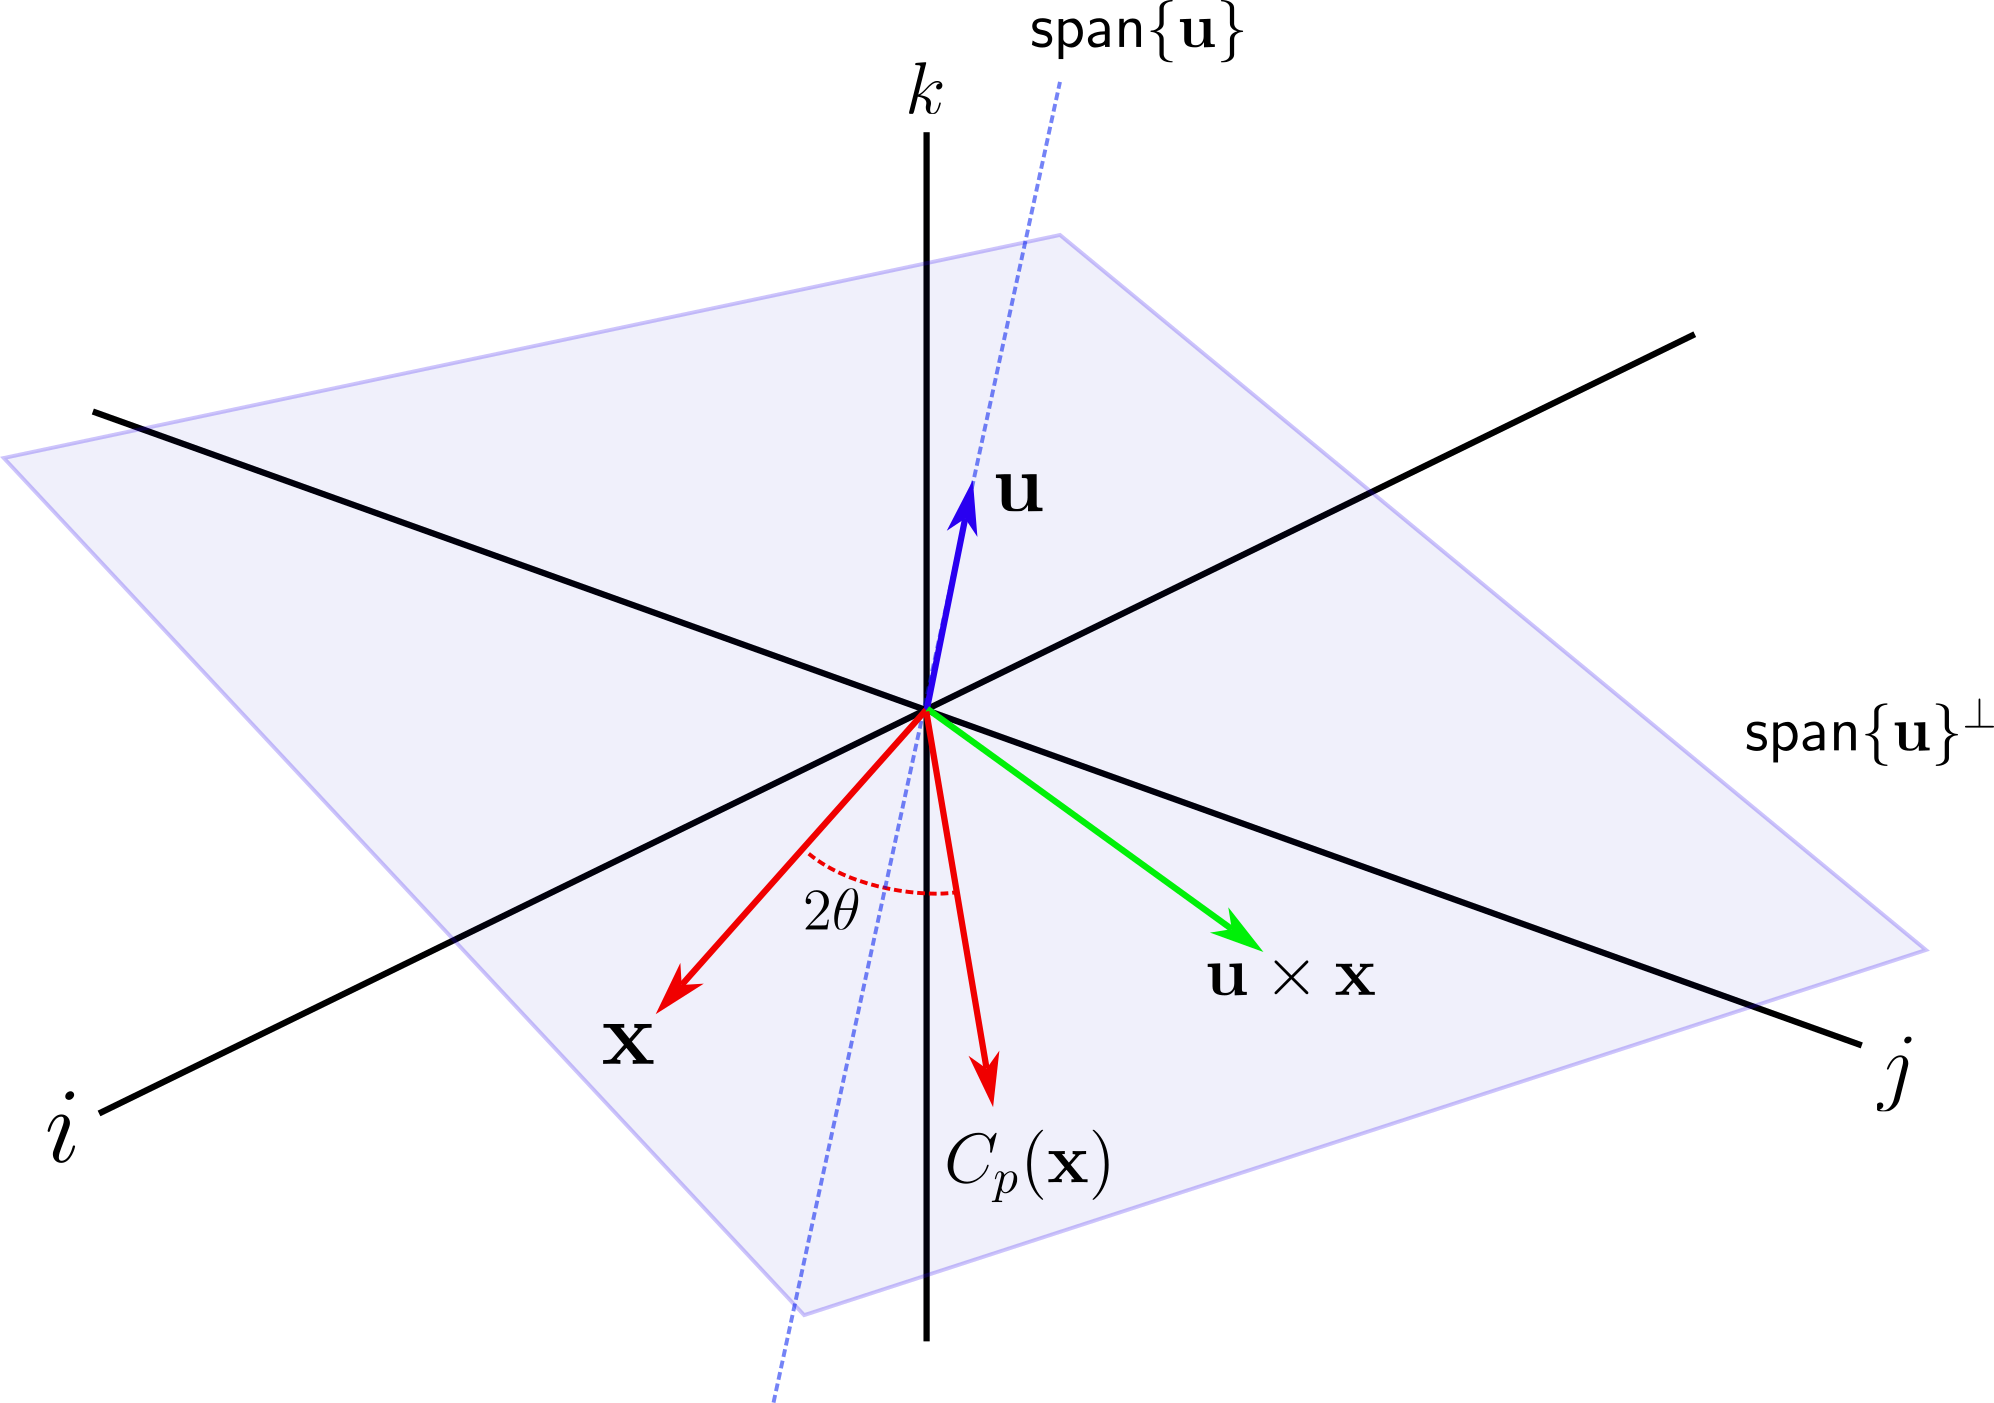
\includegraphics[width=0.8\linewidth]{quaternion.png}
    \caption{Diagram of rotation including the vectors $\vec{u},\vec{x},\vec{u}\times\vec{x}$.}
    \label{fig:quaternion}
\end{figure}

\subsubsection{Exact Sequences and Double Covers}
\begin{defn}[Exact Sequence]
Let $G_1,...,G_n$ be a list of groups, and suppose there are maps $f_0: \{1\} \to G_1, f_1 : G_1 \to G_2, ..., f_{n-1} : G_{n-1}\to G_n, f_n : G_n\to\{1\}$, where $\{1\}$ is the trivial group. That is, we have a diagram
\[1\to G_1\to\cdots \to G_n\to 1\]
Suppose these maps satisfy $\ker f_{i} = \image f_{i-1}$ for all $i=1,...,n+1$. Then we say the sequence $G_1,...,G_n$ forms an \textbf{exact sequence}.  
\end{defn}
\begin{example}
Observe that the set $\ZZ/2 = \{-1,1\}$ is a group with respect to multiplication.
Define \[f_0 : 1 \to \ZZ/2\] 
by $f_0(1) = 1$. Define
\[f_1 : \ZZ/2 \to S^3\] by $f_1(1) = 1, f_1(-1) = -1$. Define 
\[f_2 : S^3\to \SO(3,\RR)\] by $f_2(p) = C_p$, and define 
\[f_3 : \SO(3,\RR)\to 1\]
 by $f_3(R) = 1$. 

This gives us an exact sequence of maps,
\begin{equation}1\to \ZZ/2 \to S^3 \to \SO(3,\RR)\to 1\label{eq:so3exact}\end{equation}
\end{example}
\begin{defn}
Let $A,B,C$ be groups.
Let $\iota : A\to A\times C$ be given by $\iota(a)=(a,1)$, and let $p : A\times C \to C$ be given by $p(a,c) = c$. Suppose that we have an exact sequence,
\[1\to A\xrightarrow[a]{} B\xrightarrow[b]{} C \to 1\]

    Then we say this sequence \textbf{splits} if there exists an isomorphism $f : B\to A\oplus C$ so that $f\circ a = \iota$ and $p\circ f = b$. 
\end{defn}
\begin{thm}
The exact sequence \eqref{eq:so3exact} does not split. In other words, there does not exist any map $\varphi : \SO(3,\RR) \to S^3$ so that $\varphi \circ C = \One$.
\end{thm}
\begin{proof}
    Suppose $\varphi$ existed. Then $[S^3 :\image \varphi] = 2$, so $\image\varphi$ is a normal subgroup of $S^3$.

    By the first isomorphism theorem, this would mean $S^3/\image\varphi$ is isomorphic to $\ZZ/2$. Let $\rho : S^3 \to S^3/\image\varphi$ be the quotient map.

    Recall that if $u,v\in S^2$, there exists $r\in S^3$ so that $rvr^{-1} = u$. Since $\ZZ/2$ is abelian, we have $\rho(u)=\rho(rvr^{-1}) = \rho(v)$ for all $u,v\in S^2$.

    Now recall that a basis for $\HH$ is given by $\{e_0,e_1,e_2,e_3\}$. We have $\rho(e_3)=\rho(e_1)\rho(e_2)$, and since $u,e_1\in S^2$ we have $\rho(u) = \rho(e_1) = \rho(e_2)^{-1}\rho(e_3) = \rho(e_2^{-1}e_2)=1$. Therefore, $\rho(u)=1$ for all $u \in S^2$.

    Now, if $p \in S^3$, then recall that there exist $u,v\in S^2$ with $p=uv$. So $\rho(p) = 1$ as well. 

    But this means that $\rho$ is not surjective, since $\image \rho = \{1\} \neq S^3/\image\varphi$. This is a contradiction, so the proof is complete.
\end{proof}
\begin{remark*}
    We say that since this sequence does not split, and since $\ker C$ has two elements, the map $C : S^3\to \SO(3,\RR)$ is a \textbf{nontrivial double cover}.
\end{remark*}
\begin{remark*}
    As we will soon see, this is really a statement about the \textbf{spin group}, $\Spin(3) = S^3$.
\end{remark*}
Now we will return to the study of the map $K_{p,q}$. 
\begin{lemma}
    The sequence,
    \[1\to \ZZ/2\to S^3\times S^3 \xrightarrow[K]{} \to \SO(4,\RR) \to 1\]
    is exact.
\end{lemma}
\begin{proof}
    All we need is for $K$ to be surjective. 

    Topologically, we can see that since $\image K$ contains the identity, we must have $\image K \subseteq \SO(4,\RR)$.

    Furthermore, by Cartan-Dieudonn\'e theorem any $P$ in $\SO(4,\RR)$ can be written as $P = R_{u_{2m}}\circ...\circ R_{u_1}$, with each $u_i \in S^3$.

    Therefore since $K$ is a homomorphism, if we can show that $R_{u_2}\circ R_{u_1}\in \image K$ for all $u_1,u_2$ then it follows that $\SO(4,\RR) \subseteq \image K$.

    Suppose $u_1 = \pm u_2$. Then $R_{u_2}\circ R_{u_1}=\One$. So this case is done.

    Now suppose $u_1$ and $u_2$ are linearly independent. Let $u_1 = v_1$. Then there exists $v_2$ with $u_2 = \cos\theta v_1 + \sin\theta v_2$, where $\theta = \arccos(\langle u_1,u_2\rangle)$ is the angle between the two unit quaternions. Now let $x \in \RR^4$. We have,
    \begin{align*}
        R_{u_2}(R_{u_1}(x))&= x-2\langle x,u_1\rangle u_1 - 2(\langle x-2\langle x,u_1\rangle u_1,u_2\rangle)u_2
    \end{align*}
    Exercise: check that if $x \perp \Span\{u_1,u_2\}$ then $R_{u_2}(R_{u_1}(x))=x$, and if $x \in \Span\{u_1,u_2\}$ then $R_{u_2}(R_{u_1}(x))=\cos(2\theta)x+\sin(2\theta)v_3$ for some $v_3$.

    Finally we just need to show that any rotation of this form is in the image of $K$. Let $L = \Span\{u_1,u_2\}^\perp$. Then $\HH = L\oplus L^\perp$, where $P$ fixes $L$ and rotates $L^\perp$. This is done in two cases.

    First, if $1 \in L$ then $P$ must be in $\SO(3,\RR)$ and $P = K_{p,p}$ for some $P$.

    The other case: MISSING
 \end{proof}
\begin{remark*}
    This exact sequence does not split. That is, $S^3\times S^3 \to \SO(4,\RR)$ is a nontrivial double cover. We will soon see that this is a fact about spin groups, $S^3\times S^3 = \Spin(4)$.
\end{remark*}

\section{Clifford Algebras}
\subsection{Lecture 15: Clifford Algebras}
\subsubsection{Interior Product Revisited}
Recall that the interior product is defined by,
\[\hk : V\times \Lambda^k V^* \to \Lambda^{k-1} V^*\]
where,
\[v\hk\omega(u_1,...,u_{k-1}) = \omega(v,u_1,...,u_{k-1})\]
Given a metric $G$ and $a \in \Lambda^k V$, we can also set,
\[v\hk a(\alpha_2,...,\alpha_{k-1}) = a(\flat(v),\alpha_2,...,\alpha_{k-1})\]
\begin{remark*}
    Given this, we see that $v\hk v = G(v,v)$ for any $v \in V$. Therefore the interior product is a generalization of the inner product.
\end{remark*}
\begin{remark*}
    An explicit formula is given as follows. Let $\alpha = \alpha_1\wedge...\wedge\alpha_k$. Then,
    \begin{align*}v\hk\alpha(v_2,...,v_k) &=\alpha(v,v_1,...,v_{k-1})\\&= \sum_{\sigma\in S_k} \sgn(\sigma)\alpha_{\sigma(1)}(v)\alpha_{\sigma(2)}(v_2)...\alpha_{\sigma(k)}(v_k)\\
    &= \sum_{j=1}^k\sum_{\sigma\in S_{k},\sigma(1)=j} \sgn(\sigma)\alpha_{\sigma(1)}(v_1)\left(\alpha_{\sigma(2)}(v_2)...\alpha_{\sigma(k)}(v_k)\right)\\
    &= \sum_{j=1}^k (-1)^{j+1}\alpha_{j}(v_1)\sum_{\sigma\in S_{k-1}} \sgn(\sigma)\alpha_{i_{\sigma(1)}}(v_2)...\alpha_{i_{\sigma(k-1)}}(v_k) \intertext{Where  $i_1=2,...,i_{j-1} = j-1, i_{j}=j+1,...,i_{k-1}=k$.}\\
    &= \sum_{j=1}^k (-1)^{j+1}\alpha_{j}(v)\left(\alpha_1\wedge...\wedge\alpha_{j-1}\wedge\alpha_{j+1}\wedge...\wedge\alpha_k(v_2,...,v_k)\right)
    \end{align*}
    In other words,\begin{equation}
        v\hk\alpha = \sum_{j=1}^k (-1)^{j+1}\alpha_{j}(v)\;\alpha_1\wedge...\wedge\alpha_{j-1}\wedge\alpha_{j+1}\wedge...\wedge\alpha_k
    \end{equation}
    Here we have factored out the $\alpha_{\sigma(1)}(v)$ and set $j=\sigma(1)$. Then we can sum over $\sigma(1)$ separately from the other outputs, which effectively means we are summing over the permutations of $2,...,k$. Therefore we get the wedge product of all but $\alpha_{\sigma(1)}$ in the end. 
\end{remark*}
\begin{lemma}
    Let $v\in V$, $\alpha\in \Lambda^{p}V^*, \beta\in \Lambda^{q}V^*$. Then,
    \begin{equation}
        v\hk(\alpha\wedge\beta) = (v\hk \alpha)\wedge\beta + (-1)^p \alpha\wedge(v\hk\beta)
    \end{equation}
    In other words, the interior product is an \textbf{(anti)-derivation}. It obeys a ``graded" version of the Leibniz rule.
\end{lemma}
\begin{proof}
    By linearity it suffices to show this for wedge-decomposable forms. Let $\alpha = \alpha_1\wedge...\wedge\alpha_p$, $\beta = \beta_1\wedge...\wedge\beta_q$. 

    To make the proof easier, we will introduce the notation $\gamma_i = \alpha_{i},i=1,...,p$ and $\gamma_{i+k}=\beta_i,i=1,...,q$. This way, $\alpha = \gamma_1\wedge...\wedge\gamma_p$ and $\beta = \gamma_{p+1}\wedge...\wedge\gamma_{p+q}$    
    Then,
    \begin{align*}
        (v\hk\alpha)\wedge\beta &= \sum_{i=1}^p (-1)^{i+1}\gamma_i(v)\gamma_1\wedge...\wedge\gamma_{i-1}\wedge\gamma_{i+1}\wedge...\wedge\gamma_{p}\wedge\gamma_{p+1}\wedge...\wedge\gamma_{p+q}\\
        (-1)^{p}\alpha\wedge(v\hk\beta)&= (-1)^p\sum_{i=p+1}^{p+q}(-1)^{i+p+1}\gamma_i(v)\gamma_1\wedge...\wedge\gamma_p\wedge...\wedge\gamma_{i-1}\wedge\gamma_{i+1}\wedge...\wedge\gamma_{p+q}\\
        &=\sum_{i=p+1}^{p+q}(-1)^{i+1}\gamma_i(v)\gamma_1\wedge...\wedge\gamma_p\wedge...\wedge\gamma_{i-1}\wedge\gamma_{i+1}\wedge...\wedge\gamma_{p+q}
    \end{align*}
    Adding these together, we get,
    \[(v\hk\alpha)\wedge\beta+(-1)^{p}\alpha\wedge(v\hk\beta)=\sum_{i=1}^{p+q}(-1)^{i+1}\gamma_i(v)\gamma_1\wedge...\wedge\gamma_{i-1}\wedge\gamma_{i+1}\wedge...\wedge\gamma_{p+q}\]
    The right hand side is exactly $v\hk(\alpha\wedge\beta)$ as required.
\end{proof}
\begin{thm}
Let $G$ be a metric on $V$.
    Let $v\in V,\alpha\in\Lambda^{k-1}V, \beta\in\Lambda^k V$. Then,
    \begin{equation}
        G(v\wedge \alpha,\beta) = G(\alpha,v\hk \beta)
    \end{equation}
    In other words, the interior product is the \textbf{adjoint} of the exterior product.
\end{thm}
\begin{proof}
    By linearity it is enough to show that this is true for wedge-decomposable forms. Let $\alpha = \alpha_2\wedge...\wedge \alpha_{k-1}$, $\beta = \beta_1\wedge...\wedge \beta_k$. Then we have,
    \begin{align*}
        G(v\wedge\alpha,\beta) &= G(v\wedge\alpha_2\wedge...\wedge \alpha_{k-1},\beta_1\wedge...\wedge \beta_{k})\\
        &= \det\m{G(v,\beta_1)&\cdots & G(v,\beta_k)\\
        \vdots &\ddots&\vdots\\
        G(\alpha_k,\beta_1)&\cdots&G(\alpha_k,\beta_k)}\\
        &= \sum_{j=1}^k (-1)^{j+1}G(v,\beta_j)\det [G(\alpha_i,\beta_j)]_{i\neq j}\\
        &=\sum_{j=1}^k (-1)^{j+1}G(v,\beta_j)\beta_1\wedge...\wedge\beta_{j-1}\wedge\beta_{j+1}\wedge...\wedge\beta_k(\alpha_2,...,\alpha_{k-1})\\
        &=v\hk\beta(\alpha_2\wedge...\wedge\alpha_{k-1})\\
        &= G(\alpha,v\hk\beta)
    \end{align*}
    Where in line 3 we have used the cofactor expansion to sum over the first row of the overlap matrix, and from line 4 to 5 we have used the formula for the interior product derived above.
\end{proof}
\begin{lemma}
Let $G$ be a metric on $V$.
Let $w\in V$ and $\alpha\in \Lambda^k V$. Then,
\begin{equation}
    w\hk (w\wedge\alpha) = |w|^2\alpha
\end{equation}
\label{lemma:15.2}
\end{lemma}
\begin{proof}
    By the product rule for the interior product we have $w\hk(w\wedge \alpha) = (w\hk w)\wedge\alpha - w\wedge(w\hk\alpha)$. We know $w\hk w = w(\flat(w)) = G(w,w)$. So $(w\hk w)\wedge \alpha = |w|^2\alpha$.
    
    
    Therefore we just need to show that the second term vanishes. We have,
    
    \begin{align*}w\wedge(w\hk\alpha)(v_1,...,v_{k})&=\left[w\wedge \sum_{j=1}^k (-1)^{j+1}\alpha_j(w) \alpha_1\wedge...\wedge\alpha_{j-1}\wedge\alpha_{j+1}\wedge...\wedge\alpha_k\right](v_1,...,v_{k})\\
    &=\left[\sum_{j=1}^k \alpha_j(w) \alpha_1\wedge...\wedge\alpha_{j-1}\wedge w\wedge \alpha_{j+1}\wedge...\wedge\alpha_k\right](v_1,...,v_{k})\end{align*}
\end{proof}
\begin{defn}
    We define the following notation.

    Let $I_v : \Lambda^k V \to \Lambda^{k-1}V$ be given by $I_v(\alpha) = v\hk \alpha$, and let $E_v : \Lambda^k V \to \Lambda^{k-1}V$ be given by $E_v(\alpha) = v\wedge \alpha$.
\end{defn}
\begin{remark*}
    Note that $E_v^2 = I_v^2 = 0$.
\end{remark*}
\begin{cor}
    In the proof of lemma \ref{lemma:15.2} we showed that $I_v \circ E_v + E_v\circ I_v = \langle v,v\rangle\One$.
\end{cor}
\subsubsection{Quotient Algebras}
Here we will first go over the definition of a quotient algebra. The definition is almost the same as a quotient vector space, except in order for the quotient to form an algebra we will require that the denominator is more than just a vector space. We will require that it is an ideal.
\begin{defn}[Ideal of an Algebra]\index{Algebra!Ideal}\index{Ideal!Algebra}
    Let $A$ be an algebra. Then an \textbf{ideal} is a vector subspace $B$ of $A$ with the additional property that if $v\in A$ and $w \in B$ then $vw \in B$ and $wv\in B$.

    In other words, an ideal is a vector subspace which \textit{absorbs vector multiplication from the left and right}.
\end{defn}
\begin{defn}
    Let $A$ be an algebra and let $B$ be an ideal of $A$. Then the \textbf{quotient algebra} is the set of equivalence classes $[v] = \{v + b : b \in B\}$, and is denoted,
    \[A/B = \{[v] : v\in A\}\]
    Sometimes we use the notation $[v] = v+B$.
\end{defn}
\begin{remark*}
    Observe that since $B$ is an ideal, we have $wB = Bw = B$ for all $w\in A$, and $B^2 = \{bB : b \in B\} = B$, by the absorption property. Therefore,
    \[[v][w] = (v+B)(w+B) = vw+vB+wB+BB = vw + B = [vw]\]
    This means that the quotient of an algebra by an ideal is indeed a well defined algebra, and the multiplication rule from the original algebra still makes sense.
\end{remark*}

\subsubsection{The Clifford Algebra}

Recall definition \ref{defn:tensoralgebra} of the \textbf{tensor algebra}. It is given by 
\[\bigotimes V = \bigoplus_{k=0}^\infty V^{\otimes k}\]
Each element of $\bigotimes V$ is of the form $\sum_{k=0}^N Y_k$ with each $Y_k \in V^{\otimes k}$. 
\begin{example}
    Let $V = \RR^3$. Then, for example,
    \[1 + e_1 + 3e_1\otimes e_2 \otimes e_3 \in \bigotimes V\]
\end{example}
\begin{remark*}
    The set $\bigotimes V$ is a real algebra, where multiplication is given by the tensor product. The subset $\RR \subseteq \bigotimes V$ forms a subalgebra.
\end{remark*}

\begin{defn}
Let $V$ be a vector space with a metric $G(v,w)$ which we denote by $G(v,w) = \langle v,w\rangle$. The \textbf{Clifford ideal} of $V$ is the set
    \[I(V)=\left\{\sum_{k=1}^N \alpha_k \otimes(v_k\otimes v_k+\langle v_k,v_k\rangle 1)\otimes \beta_k: \quad \alpha_k,\beta_k \in \bigotimes V, v_k\in V\right\}\]
    That is, $I(V)$ is the \textbf{ideal} generated by elements of the form $v\otimes v+\langle v,v\rangle1$. 
\end{defn}
\begin{defn}[Clifford Algebra]\index{Algebra!Clifford Algebra}
Let $V$ be a vector space and let $G$ be a metric on $V$. Then the \textbf{Clifford algebra} of $V$ is the quotient,
    \begin{equation}
        \Cl(V,G) = \frac{\bigotimes V}{I(V)}
    \end{equation}
It is associative.
\end{defn}
\begin{remark*}
    The multiplication is denoted $\alpha \cdot \beta = [\alpha\otimes\beta] = \alpha\otimes\beta + I(V)$.
\end{remark*}
\begin{thm}
Let $v,w \in \Cl(V,G)$. Then,
    \begin{equation}
        v\cdot w + w\cdot v = - 2G(v,w) = -2\langle v,w\rangle
    \end{equation}
    And in particular, 
    \begin{equation}
        v\cdot v = -Q(v)=-|v|^2
    \end{equation}
\end{thm}
\begin{proof}
    Note that $(v+w)\otimes (v+w) + |v+w|^21 
 \in I(V)$ for all $v,w$. We can rewrite this to derive another identity.
    We have,
    \begin{align*}
        (v+w)\otimes (v+w) + |v+w|^21&= v\otimes w + |v|^21 +v\otimes v +  w\otimes v + |w|^21 + \langle v,w\rangle1 + \langle w,v\rangle1\\
        &= v\otimes w + w\otimes v + 2\langle v,w\rangle1 + (v\otimes v+|v|^21) + (w\otimes w+|w|^21)
    \end{align*}
    Since $v\otimes v + |v|^21$ and $w\otimes w+|w|^21$ are both elements of $I(V)$, and $I(V)$ is closed under addition,
    \[(v+w)\otimes (v+w) + |v+w|^21-v\otimes v + |v|^21-w\otimes w+|w|^21 \in I(V)\]
    Therefore, $v\otimes w + w\otimes v + 2\langle v,w\rangle \in I(V)$. In other words,
    \[
        v\cdot w + w\cdot v + 2\langle v,w\rangle = [v\otimes w + w\otimes v + 2\langle v,w\rangle1] = [0] = 0
    \]
    This completes the proof.
\end{proof}
\subsubsection{Universal Properties}
A \textbf{universal property} is a feature of a set which completely characterizes it. Before covering the universal property of the Clifford algebra, I figured it would be good to show some simpler examples.
\begin{defn}[Universal Property] \index{Universal Property!Definition}
    A property of a set $S$ with some structure (such as a group, algebra, vector space, etc structure) is called a \textbf{universal property} if any other set with the same property is isomorphic (in the sense of the aforementioned structure) to $S$.
\end{defn}

\begin{example}[Universal Property of the Product]\index{Universal Property!Products}
Let $A$ and $B$ be sets. Recall that, given the product $A\times B$, there are maps $\pi_A : A\times B \to A$ with $\pi_A(a,b)=a$, and $\pi_B : A\times B \to B$ with $\pi_B(a,b) =b$.

The universal property which completely characterizes $A\times B$ is as follows. Consider the following diagram.
\begin{center}
\begin{tikzcd}
  & D \arrow[d, "\phi"'] \arrow[ldd, "f_1"'] \arrow[rdd, "f_2"] &   \\
  & C \arrow[ld, "\pi_X"] \arrow[rd, "\pi_Y"']                  &   \\
A &                                                             & B
\end{tikzcd}
\end{center}

Suppose $C$ is a set and that there exist surjective functions $\pi_A : C\to A$ and $\pi_B : C \to B$.  

We say that $C$ is satisfies the \textbf{universal property} of $A\times B$ if for all sets $D$, and functions $f_1 : D\to A, f_2 : D \to B$, there exists a unique function $\phi : D \to C$ so that $f_1 = \pi_A\circ \phi$ and $f_2 = \pi_B \circ \phi$.

If two sets $C_1$ and $C_2$ obey the universal property, then $C_1$ and $C_2$ are in bijection. Therefore, we denote $C = A\times B$, since any two sets satisfying the universal property are essentially the same.

If we put more requirements on the arrows in the diagram, we end up with the equivalent of the cartesian product for different kinds of special sets.

For example, if $A,B,C,D$ are taken to be groups, and all the functions in the diagram are group homomorphisms, then the above universal property says that $C = A\times B$ if and only if for all groups $D$ and group homomorphisms $f_1:D\to A,f_2:D\to B$, there exists a group isomorphism $\phi : D \to C$ satisfying the equations $f_1 = \pi_A\circ\phi$ and $f_2=\pi_B\circ\phi$. 

Similarly we can construct the equivalent of the product for vector spaces, algebras and so on.
\end{example}
\begin{thm}[Universal Property of the Clifford Algebra]\index{Universal Property!Clifford Algebra}
    Let $V$ be a vector space over $\RR$ and let $A$ be a unital algebra over $\RR$. 

    Suppose that $\phi : V \to A$ is a linear map, and suppose $\phi(x)\phi(x) = -G(x,x)1_A$ for all $x \in V$.

    Suppose $B$ is an algebra, and that there exists an injective linear map $\iota : V \to B$, and a unique algebra homomorphism $\tilde{\phi}:B\to A$ so that $\tilde{\phi}\circ\iota =\phi$. Then there is an algebra isomorphism between $B$ and the Clifford algebra of $V$.

    That is, $B\cong \Cl(V,G)$ iff for all unital associative algebras $A$ and all linear maps $\phi : V\to A$ with $\phi(x)\phi(x)=-G(x,x)1_A$, there exists a unique diagram
    \begin{center}
\begin{tikzcd}
V \arrow[d, "\iota"'] \arrow[r, "\phi"] & A \\
B \arrow[ru, "\tilde{\phi}"']           &  
\end{tikzcd}
    \end{center}
    Where $\iota$ is injective, $\tilde{\phi} = \phi\circ\iota$, and $\tilde{\phi}$ is a homomorphism.
\end{thm}
\begin{proof}
    We must first show that $\bigotimes V/I(V)$ satisfies this property, and then show that if $B$ satisfies the same property then $B\cong \bigotimes V/I(V)$.

    Let $\phi:V\to A$ be a linear map. 
    
    First note that any algebra homomorphism $g : \bigotimes V \to A$ must satisfy the formula, $g(v_1\otimes...\otimes v_k) = g(v_1)...g(v_k)$.

    We then define an algebra homomorphism $\hat{\phi} : \bigotimes V \to A$  by the formula $\hat{\phi}(v_1\otimes...\otimes v_k) = \phi(v_1)...\phi(v_k)$ for all $v_1,...,v_k$, and then extend it by linearity. 
    
    We can see that $\hat{\phi}(v)=\phi(v)$, so $\hat{\phi}|_{V} = \phi\circ\iota_0$, where $\iota_0 : V \to \bigotimes V$ is the inclusion map.

    Suppose that we had any other algebra homomorphism $g : \bigotimes V \to A$ which satisfied $g|_V = \phi\circ \iota_0$. Then we would have $g(v) = \phi(v)$, so 
    \begin{align*}\hat{\phi}(v_1\otimes...\otimes v_k) &= \phi(v_1)...\phi(v_k) \\&= g(v_1)...g(v_k)\\&=g(v_1\otimes ...\otimes v_k)\end{align*}
    By linearity, we see that $\hat{\phi} = g$. Therefore $\hat{\phi}$ is unique.

    Since $\phi(x)\phi(x) = -|x|^21$, we have $\phi(x\otimes x + |x|^21) = 0$. Therefore $I(V) \subseteq \ker \phi$. Let $q : \bigotimes V \to \bigotimes V/I(V)$ be the quotient map, and let $\tilde{\phi} : \bigotimes V/I(V) \to A$ be given by $\tilde{\phi}(v_1...v_k) = \phi(v_1)...\phi(v_k)$. Then since $\ker \phi$ contains $I(V)$ we have $\tilde{\phi} = q\circ \hat{\phi}$. Since $\hat{\phi}$ is unique, $\tilde{\phi}$ is the unique extension of $\phi$ to $\Cl(V)$. That is, we have shown that $\bigotimes V/I(V)$ satisfies the universal property of $\Cl(V)$. This completes the proof of the first half.

    Now we must prove that if $A$ is any other algebra which satisfies the universal property of the Clifford algebra, then $A$ is isomorphic to $\bigotimes V/I(V)$.

    First, we have that any linear map $\varphi : V \to A$ with $\phi(x)\phi(x) = -|x|^2$ has a unique extension to an algebra homomorphism $\varphi : \Cl(V)\to A$.
\end{proof}
\begin{cor}
    Let $\{e_1,...,e_n\}$ be an orthonormal basis for $V$. That is, $\langle e_i,e_j\rangle=\pm\delta_{ij}$. Suppose $\varphi : V \to A$ satisfies $\varphi(e_j^2) = -|e_j|^2$ and $\varphi(e_i)\varphi(e_j)+\varphi(e_j)\varphi(e_i)=0$. Then $\varphi$ has a unique extension to $\varphi : \Cl(V)\to A$.
\end{cor}
\begin{proof}
    We have $\varphi(e_i\otimes e_i + |e_i|^21) = 0$ by definition. Using the polarization identity and linearity, one can expand each term in $x\otimes y + y \otimes x + 2\langle x,y\rangle 1$ in terms of a basis, before applying $\varphi$ to show that $\varphi(x)\varphi(y)+\varphi(y)\varphi(x)=-2\langle x,y\rangle 1$. So $\ker \varphi$ contains $I(V)$. This completes the proof.
\end{proof}
\begin{thm}
    The vector space $\Lambda^\bullet V$ is canonically isomorphic as a vector space to $\Cl(V)$.

    Furthermore, if $v,w \in \Cl(V)$, then $vw = v\wedge w -v\hk w$.
\end{thm}
We will delay the proof until after some remarks.
\begin{remark*}
    Let $\phi : \Lambda^\bullet V\to \Cl(V)$ be the canonical isomorphism. Let $\iota : V \to \Cl(V)$ be the inclusion map. Then $\iota\circ \phi$ is injective.
\end{remark*}
\begin{remark*}
    It is not isomorphic as an algebra to $\Cl(V)$ because they have different multiplications.
\end{remark*}
\begin{defn}[Clifford Product]
    When we interpret elements $v,w$ of $\Cl(V)$ as elements of $\Lambda^\bullet V$, the product $vw$ is referred to as the \textbf{Clifford product}.
\end{defn}
\begin{remark*}
    The Clifford algebra is not a graded algebra (recall Definition \ref{defn:gradedalgebra}) since the Clifford product of two $k$-forms is not a $k+\ell$-form.
\end{remark*}
\begin{remark*}
    Some books define $\Cl(V)$ to be generated by the ideal $I(V) = \langle v\otimes v - |v|^21\rangle$ instead, in which case the Clifford product is $vw = v\wedge w + v\hk w$. This is equivalent to replacing the metric $G$ with $-G$, or replacing the signature $(p,q)$ with $(q,p)$.
\end{remark*}
Now we will get to the proof of the theorem.
\begin{proof}
    We first show that the restriction of the quotient map $q : \bigotimes V \to \Cl(V)$ to the subspace $\Lambda^\bullet V \subset\bigotimes V$ is surjective. That is, every equivalence class can be represented by a skew-symmetric tensor.

    For a tensor of degree $0$ or $1$ this is trivial. Let $\beta\in \bigotimes V$ be decomposable. Then 
    \[\beta = \frac{1}{2}(x\otimes y + y \otimes x) + \frac{1}{2}(x\otimes y - y\otimes x)\]
    Adding and subtracting $G(x,y)1$, we can get this to be in the form
    \[\beta=\frac{1}{2}(x\otimes y+y\otimes x+2G(x,y)1)-G(x,y)1\]
    Where the first term is an element of $I(V)$ and the second term is an element of $\Lambda^0 V$.

    Inductively we can show that any decomposable $k$-tensor can be written as something in $I(V)$ plus something in $\Lambda^0 V$.

    We have a surjection from $\Lambda^\bullet V$ to $\Cl(V)$. Now we need to construct a surjection from $\Cl(V)$ to $\Lambda^\bullet V$. 

    We will use the universal property to construct a map $\varphi : V \to \mathsf{End}(\Lambda^\bullet V)$. First we remark that $\mathsf{End}(\Lambda^\bullet V)$ is an algebra over $\RR$ with identity. Then set $\varphi(x) = [E_x - I_x]$ for $x \in V$. Then $\varphi(v)(w)=v\wedge w - w\wedge v$ and so $\varphi(v)\circ\varphi(w)=[E_x-I_x]^2=-|x|^2\One$. So $\varphi$ extends uniquely to an algebra homomorphism $\varphi : \Cl(V) \to \mathsf{End}(\Lambda^\bullet V)$.

    Now let us define $\psi : \mathsf{End}(\Lambda^\bullet V) \to \Lambda^\bullet V$ by $\psi(A) = A(1)$. Observe that this map is linear. Let us define $L = \frac{1}{k!}\psi\circ \varphi : \Cl(V) \to \Lambda^\bullet V$, which is linear.

    Let $\alpha = v_1\wedge...\wedge v_k \in \Lambda^\bullet V$. We have
    \begin{align*}
        L\circ q(\alpha) &= L([\alpha])\\
        &= L([v_1\wedge...\wedge v_k])\\
        &= L\left(\left[\sum_{\sigma \in S_k} \sgn(\sigma)\;v_{\sigma(1)}\otimes...\otimes v_{\sigma(k)}\right]\right)\\
        &= L\left(\sum_{\sigma \in S_k} \sgn(\sigma)\;v_{\sigma(1)}... v_{\sigma(k)}\right)\\
        &= \frac{1}{k!}\psi\circ\varphi\left(\sum_{\sigma \in S_k} \sgn(\sigma)\;v_{\sigma(1)}... v_{\sigma(k)}\right)\\
        &= \frac{1}{k!}\psi\left(\sum_{\sigma \in S_k} \sgn(\sigma)\;(E_{v_{\sigma(1)}}-I_{v_{\sigma(1)}})...(E_{v_{\sigma(k)}}- I_{v_{\sigma(k)}})\right)\\
        &= \frac{1}{k!}\sum_{\sigma \in S_k} \sgn(\sigma)\;(E_{v_{\sigma(1)}}-I_{v_{\sigma(1)}})...(E_{v_{\sigma(k)}}- I_{v_{\sigma(k)}})(1)\\
        &= \frac{1}{k!}\sum_{\sigma \in S_k} \sgn(\sigma)\;(E_{v_{\sigma(1)}}-I_{v_{\sigma(1)}})...(E_{v_{\sigma(k-1)}}- I_{v_{\sigma(k-1)}})(v_{\sigma(k)})
        \intertext{Note that $(E_{v_{\sigma(k-1)}}- I_{v_{\sigma(k-1)}})(v_{\sigma(k)})=v_{\sigma(k-1)}\wedge v_{\sigma(k)}-G(v_{\sigma(k-1)},v_{\sigma(k)})$. In the above sum, the term $(v_{\sigma(k-1)},v_{\sigma(k)})$ will always appear twice, with opposite signs. Since $G$ is symmetric, this means all the scalar terms vanish.}
        &= \frac{1}{k!}\sum_{\sigma \in S_k} \sgn(\sigma)\;v_{\sigma(1)}\wedge...\wedge v_{\sigma(k)} \\
        &= v_1\wedge...\wedge v_k
    \end{align*}
    Therefore, $L\circ q$ is an isomorphism. Since $q$ is surjective, this means $L$ has to be injective. Therefore, we have an injection $L : \Lambda^\bullet V \to \Cl(V)$.

    Finally, we have $\varphi(x\alpha) = \varphi(x)\varphi(\alpha)$, so $\psi(\varphi(x\alpha))=\varphi(x\alpha)1 = \varphi(x)\psi(\varphi(\alpha))$. So $L(x\alpha) = x\wedge L(\alpha) - x\hk L(\alpha)$. Therefore, for any $x \in V, \alpha \in \Lambda^\bullet V$ we know that $L$ maps $x\alpha$ to $x\wedge \alpha - x \hk \alpha$. We also know 
    \begin{align*}
        q\circ L(v_1...v_k)&=q(v_1\wedge...\wedge v_k)\\
        &= v_1...v_k
    \end{align*}
    So $q \circ L = \One$ and $L\circ q = \One$. This means $q=L^{-1}$. In other words, $L$ is an isomorphism.
\end{proof}
\begin{remark*}
    We can therefore just think of $\Cl(V)$ as the vector space $\Lambda^\bullet V$ along with the new multiplication rule $v\alpha = v\wedge \alpha - v\hk \alpha$ for $v\in V$ and $\alpha\in \Lambda^\bullet V$.
\end{remark*}
\begin{example}
    If $\alpha = 1$ then $v\alpha = v$.

    If $v,w\in V$ then $vw = v\wedge w - \langle v,w\rangle 1$.

    If $v,w,u \in V$ then 
    \begin{align*}u(vw) &= u(v\wedge w-\langle v,w\rangle 1)\\ &= u\wedge v \wedge w - \langle v,w\rangle u - u\hk v \wedge w + u \hk \langle v,w\rangle 1\\
    &= u\wedge v \wedge w - \langle v,w\rangle u - \langle u,v\rangle w + \langle u,w\rangle v\end{align*}
\end{example}

The Clifford algebra has a lot of extra structure, such as involutions, automorphisms, and anti-automorphisms. Also, a special case of the universal property is when $A$ is also a Clifford algebra.

\begin{thm}
    Let $V_1,G_1$ and $V_2,G_2$ be two vector spaces with metrics. Then for each isometry $P : V_1\to V_2$ we have a unique extension to an algebra homomorphism $\Cl(V_1)\to \Cl(V_2)$. 
\end{thm}
\begin{proof}
    We have $P(x)P(x) = -|P(x)|^2 1 = -|x|^2 1$. So $P$ satisfies the universal property.
\end{proof}

\begin{remark*}
    Each linear map $T : V_1 \to V_2$ has a unique extension to an algebra homomorphism $T : \Lambda^\bullet V_1 \to \Lambda^\bullet V_2$ (given by the exterior power). This extension is the same as the extension to a map $\Cl(V_1)\to \Cl(V_2)$ as long as $T$ preserves the metric.
\end{remark*}
\begin{remark*}
    If $Q : V_2 \to V_3$ is another isometry then $Q\circ P$ is an isometry and has a unique extension to a map $\tilde{Q\circ P} :\Cl(V_1)\to \Cl(V_3)$. It is equal to $\tilde{Q}\circ\tilde{P}$.
\end{remark*}

\begin{defn}
    Let $\Aut_{\textsf{alg}}(\Cl(V))$ denote the set of all algebra automorphisms of $\Cl(V)$.

    The set of \textbf{Clifford automorphisms} is the set of all automorphisms which map $V$ into $V$, and is denoted $\Aut(\Cl(V))$.\index{Automorphism!Clifford Automorphism}
\begin{equation}
    \Aut(\Cl(V)) = \{P \in \Aut_{\textsf{alg}}(\Cl(V)) | P(V)\subseteq V\}
\end{equation}
\end{defn}

\begin{thm} The set of Clifford automorphisms of $V$ is equal to the orthogonal group of $V$. In other words $\Aut(\Cl(V)) = \Orth(V)$.
\end{thm}
\begin{proof}
    Suppose $P \in \Orth(V)$. Then $P$ maps $V$ to $V$ and preserves the inner product. Therefore, $P$ extends to a map $\Cl(V) \to \Cl(V)$, and since $P$ is invertible the extension is invertible. So $P$ is a Clifford automorphism.

    Now suppose $P \in \Aut(\Cl(V))$. Then \begin{align*}\langle P(x),P(x)\rangle &= -P(x)P(x) \\&= -P(x^2) \\&= P(-x^2) \\&= P(\langle x,x\rangle 1) \\&= \langle x,x\rangle\end{align*}
    So $P \in \Orth(V)$.

    Therefore every Clifford automorphism is an extension of an isometry of $V$.
\end{proof}
\subsubsection{Clifford Involutions}
We will now see that $\Cl(V)$ comes equipped with a special Clifford automorphism and two anti-automorphisms.

\begin{defn}[Canonical Clifford Automorphism]
    The isometry $P(v) = -v$ extends to an automorphism of $\Cl(V)$. We will denote the extension by the tilde symbol, so $\tilde{P}(\alpha) = \tilde{\alpha}$. It is called the canonical Clifford automorphism. Notice that $-(-v)=v$, so $\tilde{\tilde{v}}=v$. So the canonical automorphism is an involution.
\end{defn}
\begin{defn}[Even/Odd parts of the Clifford Algebra]
    The even/odd parts of the Clifford algebra are defined by,
    \begin{align}
        \Cl^{\textsf{even}}(V) &=\{\alpha \in \Cl(V) : \tilde{\alpha}=\alpha\}
        \\
        \Cl^{\textsf{odd}}(V) &=\{\alpha \in \Cl(V) : \tilde{\alpha}-=\alpha\}
    \end{align}
\end{defn}
\begin{lemma}
    Since $\alpha = \frac{1}{2}(\alpha+\tilde{\alpha}) + \frac{1}{2}(\alpha-\tilde{\alpha})$ we have
    \[\Cl(V) = \Cl^{\textsf{even}}(V)\oplus \Cl^{\textsf{odd}}(V)\]
\end{lemma}
Recall that $\Lambda^\bullet V$ is a graded algebra, and we have $\Lambda^\bullet V = \Lambda^{\textsf{even}}V\oplus \Lambda^{\textsf{odd}}V$, where $\Lambda^{\textsf{even}}V = \bigoplus \Lambda^{2k}V$ and $\Lambda^{\textsf{odd}}V = \bigoplus \lambda^{2k+1}V$.
\begin{lemma}
There exists vector space isomorphisms $\Lambda^{\textsf{even}}V \cong \Cl^{\textsf{even}}(V)$ and $\Lambda^{\textsf{odd}}V \cong \Cl^{\textsf{odd}}(V)$.
\end{lemma}
\begin{proof}
    Let $\{e_1,...,e_n\}$ be an orthonormal basis. Then $e_{i_1}...e_{i_k} = e_{i_1}\wedge...\wedge e_{i_k}$ since $e_{i_j}\hk e_{i_\ell}=0$ for all $j,\ell$. This means $\bigtilde{e_{i_1}...e_{i_k}} = \tilde{e}_{i_1}...\tilde{e}_{i_k} = (-1)^k e_{i_1}...e_{i_k}$. So the parity of the form $\alpha = e_{i_1}...e_{i_k}$ with respect to the canonical automorphism is the same as the parity of $\alpha$ with respect to the grading on $\Lambda^k V$. Extending by linearity completes the proof.
\end{proof}
\begin{defn}[Canonical Anti-Automorphism]
Consider the map $T : \bigotimes V \to \bigotimes V$ defined by,
\[T(v_1\otimes...\otimes v_k) = v_k\otimes v_{k-1}\otimes...\otimes v_2\otimes v_1\]
That is, it reverses the order of all components. This map is clearly an involution, and we can also see that it is an anti-automorphism with respect to the tensor product since $T(\alpha\otimes \beta) = T(\beta)\otimes T(\alpha)$. We write $T(\alpha) = \bigcheck{\alpha}$.
\end{defn}

\subsection{Lecture 16: Symmetries and Automorphisms of Clifford Algebras}
\subsubsection{Clifford Involutions (Continued)}
\begin{lemma}
Let $T(\alpha) = \bigcheck{\alpha}$ and $P(\alpha) = \bigtilde{\alpha}$. Then $T\circ P \circ T$ is an automorphism. Furthermore, since $(T\circ P \circ T)|_V = P|_V$, by uniqueness we see that $T\circ P \circ T = P$.  
\end{lemma}
\begin{defn}[Hat Anti-Automorphism]
    Let $T(\alpha) = \bigcheck{\alpha}$ and $P(\alpha) = \bigtilde{\alpha}$. Then we define $\bighat{\alpha} = T(P(\alpha))$. 
\end{defn}
\begin{remark*}
    By the above lemma, $T(P(\alpha))=P(T(\alpha))$. That is, $\bighat{\alpha}=\bigcheck{\bigtilde{\alpha}}=\bigtilde{\bigcheck{\alpha}}$.
\end{remark*}
\begin{thm}
    Let $a \in \Cl(V)$ be of degree $k$. Then $\bigtilde{a}=\pm a,$ $ \bigcheck{a}=\pm a,$ $\bighat{a}=\pm a$, where the signs are determined by $k$ according to the following table,
    \begin{center}
    \begin{tabular}{c|cccc}
         $k\mod 4$ & 0 &1&2&3  \\\hline
         $\sim$& +&-&+&-\\
         $\vee$&+&+&-&-\\
         $\wedge$&+&-&-&+
    \end{tabular}
    \end{center}
    \label{thm:kmod4}
\end{thm}
\begin{proof}
    Write down an orthonormal basis, and check directly.
\end{proof}
These involutions we have discussed have some important properties with respect to the metric induced on $\Cl(V)$ by the metric on $V$.
\begin{remark*}
Recall that the metric $G$ on $V$ induces a metric on $\Lambda^\bullet V$ (see equation \ref{eq:defn_induced_metric}). Since $\Lambda^\bullet V \cong \Cl(V)$ as vector spaces, we therefore also have a metric on $\Cl(V)$.
\end{remark*}
\begin{remark*}
    If $\{e_1,...,e_n\}$ is an orthonormal basis for $V$ then $\{e_{i_1}\cdot...\cdot e_{i_k} | 1\leq i_1,...,i_k\leq n\}$ is an orthonormal basis for $\Cl(V)$.
\end{remark*}
\begin{thm}
    Let $a,b\in \Cl(V)$. Then,
    \begin{align*}
        G(a,b) &= G(1,a\bighat{b})\\
        G(a,b) &= G(1,b\bighat{a})
    \end{align*}
\end{thm}
\begin{proof}
    Check directly using the aforementioned orthonormal basis.
\end{proof}
\begin{cor}
    The map $L_a : \Cl(V)\to \Cl(V)$ defined by $L_a(b)=ab$ satisfies $L_a^\dagger = L_{\bighat{a}}$. In other words, left-multiplication by $a$ is adjoint to left-multiplication by $\bighat{a}$.
\end{cor}
\begin{proof}
    \begin{align*}G(ab,c) &= G(1,\bighat{ab}c) \\&= G(1,\bighat{b}\bighat{a}c) \\&= G(b,\bighat{a}c)\end{align*}
\end{proof}
\begin{cor}
    Let $a = v_1...v_k$. Then $|a|^2 = G(a,a) = |v_1|^2...|v_k|^2$.
\end{cor}
\begin{proof}
Recall that Clifford multiplication satisfies $-v^2 = |v|^21$. Therefore we have,
    \begin{align*}
        \bighat{a}a &= \bighat{v_1...v_k}v_1...v_k\\
        &= (-v_k)...(-v_1)v_1...v_k\\
        &= |v_1|^2...|v_k|^2
    \end{align*}
\end{proof}
\begin{thm}[Hadamard Identity]
    Let $v_1,...,v_k$ be linearly independent. Then,
    \begin{equation}
        |v_1|^2 ... |v_k|^2 = |v_1\wedge...\wedge v_k|^2 + \sum_{j=1}^{k-1}|\pi_j(v_1...v_k)|^2
    \end{equation}
    Where $\pi_j(v_1...v_k)$ is the projection of $v_1...v_k$ onto $\Lambda^j V\subset\Lambda^\bullet V=\Cl(V)$.
\end{thm}
\begin{cor}[Hadamard Inequality]\index{Theorem!Hadamard Inequality}
Suppose $G$ is a positive definite metric.
    The above equation then implies that
    \begin{equation}
        |v_1\wedge...\wedge v_k|\leq |v_1|...|v_k|
    \end{equation}
    This is often referred to as the Hadamard inequality.\index{Hadamard Inequality}
\end{cor}
\begin{proof}
    Note that by definition,
    \[\sum_{j=1}^{k}\pi_j(v_1...v_k) = v_1...v_k\]
    Since each $\Lambda^\bullet V$ is an orthogonal direct sum over $j$, we therefore have
    \[\left|\sum_{j=1}^{k}\pi_j(v_1...v_k)\right|^2  = |v_1\wedge...\wedge v_k|^2 + \sum_{j=1}^{k-1}|\pi_j(v_1...v_k)|^2\]
    as required.
\end{proof}
\subsubsection{Clifford Algebras as Subspaces of Clifford Algebras}
\begin{defn}
    We define the following notation,
    \[\RR^{p,q} = (\RR^{p+q},G)\]
    Where $G$ is any metric of signature $(p,q)$.
\end{defn}
\begin{defn}
    We define the following notation,
    \[\Cl(p,q) = \Cl(\RR^{p,q})\]
\end{defn}
\begin{remark*}
    Up to isometry it does not matter what specific metric $G$ we choose.
\end{remark*}
\begin{physics*}
    One of the most commonly used vector spaces in physics is $\RR^{3,1}$. This is commonly referred to as \textbf{Minkowski space}.
\end{physics*}

Let $e_0,e_1,...,e_p,e_{p+1},...,e_{p+q}$ be the standard basis of $\RR^{p+1,q}$, where $e_{p+1},...,e_q$ are the negative definite components and $e_0,...,e_p$ are the positive definite components. Let us define a map $\phi : \RR^{p,q} \to \Cl(p+1,q)$ by the formula $\phi(e_j) = e_0e_j$, where $j=1,...,n$. Then,
\[\phi(e_i)\phi(e_i) = e_0e_ie_0e_j = -e_0^2 e_i^2 = e_i^2 = -|e_i|^2 1\]
\[\phi(e_i)\phi(e_j) = e_ie_j = -\phi(e_j)\phi(e_i)\]
By the universal property, $\phi$ extends to a unique algebra homomorphism $\phi : \Cl(p,q) \to \Cl(p+1,q)$.

Similarly, suppose $e_0,...,e_p,e_{p+1},...,e_{p+q}$ is the standard basis of $\RR^{p,q+1}$ where now $e_0$ is part of the negative-definite subspace. Suppose we define a map $\psi : \RR^{p,q} \to \Cl(p,q+1)$ by $\psi(e_j) = e_0 e_j$. Then $\psi$ extends to a unique algebra homomorphism $\phi : \Cl(p,q) \to \Cl(q,p+1)$.
\begin{thm}
We have,
\begin{enumerate}
    \item The map $\phi$ defined in the above paragraph is an isomorphism from $\Cl(p,q)$ to $\Cl^{\textsf{even}}(p+1,q)$.
    \item The map $\psi$ is an isomorphism from $\Cl(p,q)$ to $\Cl^{\textsf{even}}(q,p+1)$.
\end{enumerate}
\end{thm}
\begin{proof}
    Since $\phi(e_j) = e_0e_j$, it is clear that $\phi$ takes elements of $V$ to even elements of the Clifford algebra. 
    
    Next, notice that $e_ie_j = \pm e_0 e_i e_0 e_j=\pm \phi(e_ie_j)$, so $\phi$ is surjective. 

    Furthermore, since $\phi$ simply inserts copies of $e_0$ into a given input, we have that $\hat{\phi}(\alpha) = \phi(\hat{\alpha})$ since the order doesn't matter, and the sign pulls out.

    Finally, we note that $\phi$ sends even elements to even elements, since it would insert an even number of $e_0$s into a given input which all cancel. Additionally, when we act $\phi$ on an odd element (of degree $k$ for example), we get an odd number of $e_0$'s, so all but one cancel and the result is an element of degree $k+1$. So the output of $\phi$ always has even degree.

    Therefore we see that since $\phi$ is surjective, its' image is exactly $\Cl^{\textsf{even}}(p+1,q)$, which completes the proof.

    The proof for the other map is identical, except we see that since $e_0$ is part of the negative definite part of $\RR^{p,q+1}$ the definiteness of the output of $\phi$ always gets swapped. This is why the output is $\Cl^{\textsf{even}}(q,p+1)$.
\end{proof}
\subsubsection{Center and Twisted Center of  Clifford Algebras}
\begin{defn}[Twisted Center]\index{Algebra!Twisted Center}
Recall that the center of $\Cl(V)$ is the set of all elements of $\Cl(V)$ which commute with every other element of $\Cl(V)$,
\[\cent(\Cl(V)) = \{a \in \Cl(V) : ab = ba\;\forall\, b\in \Cl(V)\}\]
We similarly define the \textbf{twisted center} of $\Cl(V)$ to be all the elements which anti-commute with everything else,
\[\twcent(\Cl(V)) = \{a\in \Cl(V) : ab = -ba \;\forall\,b\in\Cl(V)\}\]
\end{defn}
\begin{thm}
We have,
\begin{enumerate}
    \item If $\dim V = n$ is even, then $\cent(\Cl(V)) = \Lambda^0 V$ and $\twcent(\Cl(V)) = \Lambda^n V$.
    \item If $\dim V = n$ is odd, then $\cent(\Cl(V)) = \Lambda^0 V \oplus \Lambda^n V$ and $\twcent(\Cl(V)) = \{0\}$.
\end{enumerate}
\end{thm}
\begin{proof}
    Let $v \in V$ be non-null. 
    We say an element $x\in \Cl(V)$ does not involve $v$ if there is no way to write $x = \sum x_i$ where $x_i = x_{i1}...v...x_{ik}$ for some $i,k$. That is, $x$ does not involve $v$ if the value of $x$ does not depend at all on the value of $v$.
    
    Let $a\in \Cl(V)$ and set $a = b + vc$ where $b$ and $c$ don't involve $v$. Then 
    \begin{align*}av &= (b+vc)v=bv+vcv\\
    va &= vb+v^2c = vb-|v|^2c\end{align*}
    
    Suppose $a$ and $b$ are even while $c$ is odd. Then 
    \begin{align*}av &= vb + |v|^2 c\\
    va &= vb - |v|^2 c
    \end{align*}
    
    From this we see that $va = av$ if and only if $c=0$ (in other words, $a$ does not involve $v$). Similarly $va=-av$ iff $b=0$ (which would mean $a$ involves $v$).

    Now suppose $a$ and $b$ are odd, while $c$ is even. Then
    \begin{align*}
        av &= -vb-|v|^2 c\\
        va &= vb - |v|^2 c
    \end{align*}
    So $av = va$ iff $b=0$, and $av=-va$ iff $c=0$.

    Overall, if $a$ is even and $a \in \cent(\Cl(V))$ then $av=va$ for all $v$, which means that $a$ can't possibly involve $v$. So there is no way to decompose $a$ in terms of vectors, which means $a$ must be a scalar. In other words, $a \in \Lambda^0 V$ as required.

    Similarly, suppose $a$ is odd and $a \in \cent(\Cl(V))$. Then $av=va$ for all $v$, which means that $a$ must involve $v$ for all $v$. In other words, $a$ can be decomposed into a product of all linearly independent vectors. So $a \in\Lambda^n V$. Furthermore, since $a$ is odd, this means $a$ can only be nonzero if $n$ is odd. 

    Therefore, we have shown that $\cent(\Cl(V)) = \Lambda^0 V$ if $n$ is even and $\cent(\Cl(V)) = \Lambda^0 V \oplus \Lambda^n V$ if $n$ is odd.

    Finally, by the exact same argument we see that if $a$ is even and $a\in \twcent(\Cl(V))$ then $a$ must involve all vectors $v$, which means $a \in \Lambda^n V$ and so $n$ must be even for $a$ to be nonzero. Similarly if $a$ is odd then $av=-va$ iff $a$ does not involve any vectors, which means that $a$ is either a scalar or zero. Since scalars have even degree, $a$ must be zero. This completes the proof.
\end{proof}


\subsection{Lecture 17: The Spin Group and Pin Group}
\iffalse
\subsubsection{Self-Dual and Anti-Self-Dual Forms}

\begin{remark*}
Let $\mu$ be a metric-compatible orientation (i.e. a volume form) on $\RR^{p,q}$. Recall that this means $G(\mu,\mu)=|\mu|^2 = (-1)^q$. Then by Theorem \ref{thm:kmod4} we know that $\bighat{\mu} = \pm \mu$ depends only on $p+q\mod 4$. So $\mu\mu = \pm \bighat{\mu}\mu = \pm |\mu|=\pm 1$, where the sign depends on $n,p,$ and $q$.
\end{remark*}

\begin{lemma}
Let $\mu$ be a volume form on $\RR^{p,q}$. Then,
\begin{enumerate}
    \item $\mu^2 = 1$ if $p-q=0 \mod 4$ or $p-q=3\mod 4$.
    \item $\mu^2 = -1$ if $p-q=1\mod 4$ or $p-q=2\mod 4$.
\end{enumerate}
\end{lemma}
\begin{proof}
We have $\mu = e_1...e_n$ for some orthonormal basis $\{e_1,...,e_n\}$. This means $\bigcheck{\mu}\mu = (-1)^p$.

We also know that $\bigcheck{\mu} = \mu$ if $n=0$ or $1$ mod $4$ and $\bigcheck{\mu}=-\mu$ if $n=2$ or $3$ mod $4$. So if $n=2k$, then $\bigcheck{\mu}=(-1)^k\mu$ and if $n=2k+1$ then $\bigcheck{\mu} = (-1)^k\mu$ as well.

Therefore, $\mu^2 = \mu\bigcheck{\mu}(-1)^k = (-1)^{p-k}1$.

When $n$ is even, this becomes $(-1)^{(p-q)/2}$ and when $n$ is odd it becomes $(-1)^{(p-q+1)/2}$. One can now check that this gives the desired result by substituting in each of $p-q = 1,2,3,4$.
\end{proof}
\begin{remark*}
    When $p-q=1$ or $2$ mod $4$, then $\mu$ is a \textbf{complex structure} on $\Cl(p,q)$.
\end{remark*}

\begin{defn}
Let $\mu$ be an orientation satisfying $\mu^2 = 1$ and let $a\in \Cl(p,q)$
\begin{enumerate}
    \item If $\mu a = a$ we say $a$ is \textbf{self-dual}.
    \item If $\mu a = -a$ we say $a$ is \textbf{anti-self-dual}.
\end{enumerate}
The vector subspace of all self-dual forms is denoted $\Cl^+(p,q)$ and the subspace of all anti-self-dual forms is denoted $\Cl^-(p,q)$.
\end{defn}
\begin{remark*}
    The sets $\Cl^+(p,q)$ and $\Cl^-(p,q)$ are vector subspaces, but not necessarily subalgebras.
\end{remark*}
\begin{remark*}
    Since $\mu^2 = 1$ we require that $p-q=0$ or $3$ mod $4$ in order to define these subspaces.
\end{remark*}
\begin{remark*}
    By setting $a = \frac{1}{2}(a+\mu a) + \frac{1}{2}(a-\mu a)$ we see that $\Cl(p,q) = \Cl^+(p,q) \oplus \Cl^-(p,q)$.
\end{remark*}


\begin{defn}[Left/Right Ideals]\index{Algebra!Left/Right Ideal}\index{Ideal!Left/Right Ideal of Algebra}
    Let $A$ be an algebra and let $I$ be an ideal. We say $I$ is a two-sided ideal since $aI = I$ and $Ia=I$ for all $a\in A$.

    A weaker definition is that of left and right ideals. $I$ is said to be a \textbf{right ideal} if $Ia=I$ for all $a\in A$. It is said to be a \textbf{left ideal} if $aI=I$ for all $a\in A$.
\end{defn}
\begin{lemma}
\begin{enumerate}
    \item When $p-q=3\mod 4$, the subspaces $\Cl^{\pm}(p,q)$ are two-sided ideals.
    \item When $p-q=0\mod 4$, the subspaces $\Cl^{\pm}(p,q)$ are right ideals.
\end{enumerate}
\end{lemma}
\begin{proof}
    Let $\alpha \in \Cl^{\pm}(p,q)$ and let $b \in \Cl(p,q)$. Then $\mu\alpha = \pm \alpha$, so 
    \[\mu(\alpha b) = (\mu\alpha)b = \pm \alpha b\]
    So $\alpha b \in \Cl^{\pm}(p,q)$. Therefore $\Cl^{\pm}(p,q)$ is always a right ideal.

    Now we show that if $p-q=3\mod 4$ then it is also a left ideal. Note that when this is the case, $\mu b = b\mu$, so
    \[\mu(b\alpha) = b(\mu\alpha) = b(\pm \alpha) = \pm b\alpha\]
    This completes the proof.
\end{proof}
\begin{remark*}
    Why isn't $\Cl^{\pm}(p,q)$ two-sided when $p-q=0\mod 4$? The answer is that in general, if $p-q=0\mod 4$ then $\mu(b\alpha)=\pm \bigtilde{b}\alpha$, which is not in general equal to $\pm b\alpha$.
\end{remark*}
\begin{remark*}
In fact, the algebra $\Cl(p,q)$ \textbf{only} has non-trivial two-sided ideals when $p-q=3\mod 4$, and they are always given by $\Cl^{\pm}(p,q)$ for some orientation $\mu$.
\end{remark*}

\subsubsection{Examples of Clifford Algebras}
\begin{remark*}
    Recall that $\dim \Cl(V) = 2^n$.
\end{remark*}

\begin{example}
Suppose $n=0$. Then $V = \{0\}$. We have $\Cl(V) = \RR$, where it is given the positive definite inner product $\langle a,b\rangle = ab$.
\end{example}
\begin{example}
    Let $n=1$. So $V = \Span\{e_1\}$. There are two possible signatures, $(1,0)$ and $(0,1)$. In the first case, $\langle e_1,e_1\rangle = 1$ and in the second, $\langle e_1,e_1\rangle = -1$.

    \begin{enumerate}[(i)]
    \item { The first case is the signature $(1,0)$. 

    In this case, $e_1e_1 = |e_1|^2 = -1$, so $\Cl(1,0) = \{a1 + be_1 | e_1^2 = -1\}$. This is exactly the same as the definition of the complex numbers, so we see that
    \[\CC=\Cl(1,0) \]
    }
    \item {
    The second case is the signature $(0,1)$.

    In this case, $e_1e_1 = |e_1|^2 = 1$. So we have $\Cl(0,1) = \{a1+be_1 | e_1^2 = 1 \}$. This is called the set of \textbf{Lorentz numbers} (also known as the split-complex numbers or the hyperbolic numbers). We denote it,
    \[\LL = \Cl(0,1)\]
    }
    \end{enumerate}
    \begin{remark*}
        The Lorentz numbers \textbf{do not} form a field since $(1+e_1)(1-e_1) = 1-e_1^2 = 0$.
    \end{remark*}
\end{example}
\begin{example}
    We will soon see that $\Cl(2,0) = \HH$ and that $\Cl(0,2)$ and $\Cl(1,1)$ are both isomorphic to $M_{2\times 2}(\RR)$ (although the isomorphisms are different).
\end{example}
\begin{remark*}
    Using the $k\mod 4$ which appears in many places will allow us to classify all Clifford algebras just by knowing the first few cases. This is a phenomenon called Bott periodicity.
\end{remark*}

\subsubsection{Pin Groups and Spin Groups}
For the past few lectures we have worked out many properties of Clifford algebras. Now we will examine some important subsets of Clifford algebras which form groups.

\begin{remark*}
    Let $u \in \Cl(V)$. Then if $|u|^2 \neq 0$ then $u\frac{-u}{|u|^2}=1$, so $u$ is invertible.
\end{remark*}
\begin{defn}[Group of Invertible Elements of Clifford Algebra]
    The set of all invertible elements of $\Cl(V)$ is denoted $\Cl^*(V)$. Observe that it forms a group with respect to Clifford multiplication. 
\end{defn}
\begin{remark*}
    Try not to confuse this with the dual space, $(\Cl(V))^*$.
\end{remark*}
\begin{defn}[Pin Group]
    The Pin group is defined to be the subgroup of $\Cl^*(V)$ generated by all unit vectors in $V$,
    \begin{equation}
        \Pin(V) = \{u_1...u_k : |u_i|^2 = 1\; \forall\, i=1,...,k\}
    \end{equation}
\end{defn}
\begin{remark*}
    By definition, every element $v\in \Pin(V)$ is decomposable. So every element of $\Pin(V)$ is either even or odd.
\end{remark*}
\begin{defn}[Spin Group] We define the Spin group to be all the even elements of the Pin group,
\begin{equation}
    \Spin(V) = \Cl^{\textsf{even}}(V)\cap \Pin(V)
\end{equation}
\end{defn}
\begin{lemma}
    Let $u \in V$ be a non-null vector. Then the action of a reflection $R_u$ on a vector $v\in V$ is given by $R_u(v) = -uvu^{-1}$.
\end{lemma}
\begin{proof}
    We have $uv = u\wedge v - \langle u,v\rangle$. So $uv = vu$ iff $u$ and $v$ are co-linear, since the wedge product part vanishes and we are left with the metric term which is symmetric.

    So $uvu^{-1}=v$ if $v = \lambda u$ for some $\lambda$. Furthermore, $uvu^{-1} = -v$ if $u$ and $v$ are perpendicular.  These are the two properties a reflection needs to satisfy, so we are done.
\end{proof}
The above lemma allows us to relate the Pin and Spin groups to the group of isometries of a vector space. To make this precise we will introduce some ideas from representation theory. The representation theory of the Spin group is extremely important in physics.
\begin{defn}[Representation]\index{Representation}
Let $V$ be a vector space and let $G$ be a group. Let $\GL(V)$ be the set of all invertible linear maps from $V$ to $V$. Then a \textbf{representation of} $G$ is a group homomorphism $\rho : G \to \GL(V)$.

The vector space $V$ is called a representation space of $G$, and $\dim V$ is referred to as the dimension of the representation.
\end{defn}
\begin{remark*}
    For an element of $\GL(V)$ in the image of $\rho$, we use the notation $\rho_g = \rho(g)$.
\end{remark*}
\begin{remark*}
    We call such a map a representation because it provides us with a way to represent group elements as linear maps, and group multiplication as composition of linear maps. When $V$ is finite dimensional, we can even represent group elements using invertible matrices. As you might imagine, this is extremely powerful because linear algebra makes everything easier.
\end{remark*}

\begin{defn}[Adjoint Representation]\index{Representation!Adjoint}
The \textbf{adjoint representation} of $\Cl^*(V)$ is the map $\Ad : \Cl^*(V) \to \GL(\Cl(V))$ given by 
\begin{equation}\Ad_a(b) = aba^{-1}\end{equation}
\end{defn}

\begin{defn}[Twisted Adjoint Representation]\index{Representation!Twisted Adjoint} The \textbf{twisted adjoint representation} of $\Cl^*(V)$ is the map $\bigtilde{\Ad}:\Cl^*(V) \to \GL(\Cl(V))$ given by
\begin{equation}
    \bigtilde{\Ad}_a(b) = \bigtilde{a}ba^{-1}
\end{equation}
\end{defn}
\begin{thm}
There exist exact sequences,
\begin{equation}
    1 \to \{1,-1\} \to \Pin(V) \xrightarrow{\bigtilde{\Ad}} \Orth(V) \to 1
\end{equation}
and
\begin{equation}
    1 \to \{1,-1\} \to \Spin(V) \xrightarrow{\bigtilde{\Ad}} \textsf{SO}(V) \to 1
\end{equation}
\end{thm}
\begin{proof}
    Let $u \in V$, $|u|\neq 0$. Then $R_u = \bigtilde{\Ad}_u \in \Orth(V)$ as we saw earlier. So by Cartan-Dieudonn\'e theorem, $\bigtilde{\Ad}$ surjects onto $\Orth(V)$. 
    
    Now suppose $\bigtilde{\Ad}_a$ equals the identity for some $a \in \Pin(V)$. This means $\bigtilde{a}va^{-1}=v$ for all $v\in V$. 
    
    If $a$ is odd we have $\bigtilde{a}=-a$, so $av=-va$, or in other words $a \in \twcent(\Cl(V))$ which is impossible since $\twcent(\Cl(V))$ never contains odd elements. 
    
    If $a$ is even, we have $ava^{-1}=v$, so $a\in \cent(\Cl(V))$. Since $a$ is even, we have $a \in \RR$. So $a=\pm 1$. 

    Therefore, the only way to have $\bigtilde{\Ad}_a = \One$ is to have $a=\pm 1$, so we see that $\ker \bigtilde{\Ad}|_{\Pin(V)}=\{1,-1\}$. Therefore we have shown that the first sequence is exact.

    Now recall that any element of $\SO(V)$ can be written as an even number of reflections. Since $\bigtilde{\Ad}(v)$ is a reflection for any $v \in V$, and since elements of $\Spin(V)$ are the product of an even number of vectors, we see that $\bigtilde{\Ad}(\alpha)$ is the product of an even number of reflections as required.
\end{proof}

\begin{remark*}
    The above exact sequences do not split. The proof of this is on assignment 5.
\end{remark*}


\section{Composition Algebras}
\subsection{Lecture 18: Composition Algebras}
\subsubsection{Real and Imaginary Parts of Composition Algebras}
We have seen so far that a few different composition algebras (algebras with $|ab|=|a||b|$) can be constructed using Clifford algebras. In this section we will consider these kinds of algebras in more generality, and later we will relate this back to Clifford algebras. We will see in this section that any composition algebra can be broken down into a "real" and "imaginary" part (although more work will be required to show that this has anything to do with the complex numbers or quaternions).

\begin{lemma}
    Let $A$ be a unital algebra (not necessarily associative) over $\RR$ with metric $G = \langle\cdot,\cdot\rangle$. The following are equivalent conditions for $A$ to be compositional.
    \begin{enumerate}[(i)]
    \item $|ab|^2 = |a|^2|b|^2$
    \item $\langle ac,bc\rangle = \langle a,b\rangle |c|^2$
    \item $\langle ca,cb\rangle = |c|^2 \langle a,b\rangle$
    \item $\langle ac,bd\rangle + \langle bc,ad\rangle = 2\langle a,b\rangle\langle c,d\rangle$
    \end{enumerate}
\end{lemma}
\begin{proof}
    First notice that (iv) implies (ii) and (iii), since we can set $c=d$ or $a=b$ in the equation.

    Next, we see that (i) implies (ii) by the polarization identity, $|\langle a,b\rangle c|^2 = |a+b|^2 |c|^2$

    The same argument shows that (i) implies (iii).

    Again we can use the polarization identity to show that (ii) implies (iv) and that (iii) implies (iv).

    FInally, we can set $a=b$ in (ii) or (iii) to show that (ii) implies (i) and that (iii) implies (i).
\end{proof}
\begin{defn}
    We will define a right-multiplication map by $R_a(b) = ba$, and a left-multiplication map by $L_a(b) = ab$.
\end{defn}
\begin{remark*}
    The condition (ii) in the previous lemma becomes $\langle R_c a,R_c b\rangle = |c|^2 \langle a,b\rangle$, and similar statements hold for (iii) and (iv).
\end{remark*}

Given a unital composition algebra $A$ with a metric of signature $(p,q)$ we will then define $\Re(A) = \Span\{1\}$. Then $|a1|^2 = |a|^2 |1|^2$, so $|1|^2 = 1$ as long as $p\geq 1$. This means that $\Re(A)$ is a nondegenerate subspace of $A$, and in particular we have $A = \Re(A)\oplus_\perp (\Re(A))^\perp$. We then define $\Im(A) = \Re(A)^\perp$. We therefore get $a = \Re(a)+\Im(a)$ for any $a \in A$.

Observe that $\Re(A)$ is a one-dimensional subalgebra, but $\Im(A)$ is not necessarily a subalgebra and may just be a vector subspace.

We then define a map $a \mapsto \overline{a}$ by the formula $\overline{a}=\Re(a)-\Im(a)$. This is conjugation, which we will note defines an element of $\Orth(V)$. Next time we will show that $R_a^\dagger = R_{\overline{a}}$ and $L_a^\dagger = L_{\overline{a}}$ for all $a\in A$, and that $\overline{ab}=\overline{b}\,\overline{a}$.
\subsubsection{Conjugation in Composition Algebras}
Before continuing our discussion of composition algebras we will prove the claim made at the end of the previous lecture. In this section $A$ is a unital composition algebra with metric of signature $(p,q)$.
\begin{lemma}
    Let $c \in A$. Then $R_c^\dagger = R_{\overline{c}}$ and $L_c^\dagger = L_{\overline{c}}$.
\end{lemma}
\begin{proof}
    Suppose $c \in \Re(A)$. Then $\overline{c}=c$, and furthermore, by the definition of $\Re(A)$ we have that $\langle ca,b\rangle = \langle ta,b\rangle$ for some $t\in \RR$. By linearity we can then move $t$ to the other side to get $\langle ca,b\rangle = \langle a,tb\rangle = \langle a,cb\rangle$ as required.

    Now suppose $c\in\Im(A)$. Then $\overline{c}=-c$. By property (iv), we also have $\langle a,R_cb\rangle + \langle R_ca,b\rangle=0$. So 
    \begin{align*}\langle a,R_cb\rangle &= \langle- R_ca,b\rangle \\&= \langle R_{\overline{c}}a,b\rangle\end{align*}

    By linearity the proof is complete.
\end{proof}
\begin{lemma}
    We have,
    \begin{enumerate}
    \item {
    $\overline{\overline{c}}=c$
    }
    \item {
    $\langle a,b\rangle = \Re(a\overline{b}) = \Re(\overline{a}b) = \Re(b\overline{a})=\Re(\overline{b}a)$.
    }
    \item {
    $\overline{ab} = \overline{b}\,\overline{a}$
    }
    \item {
    $\overline{a}a=a\overline{a} = |a|^2$
    }
    \end{enumerate}
\end{lemma}
\begin{proof}
    We have 
    \begin{align*}\langle a,b\rangle &= \langle a,R_b1\rangle\\& = \langle R_{\overline{b}}a,1\rangle \\&= \langle a\overline{b},1\rangle\\& = \Re(a\overline{b})
    \end{align*}
    and,
    \begin{align*}
        \langle \overline{ab},c\rangle &= \langle ab,\overline{c}\rangle\\
        &= \langle b,\overline{a}\overline{c}\rangle\\
        &=\langle bc,\overline{a}\rangle\\
        &=\langle c,\overline{b}\,\overline{a}\rangle\\
        &=\langle \overline{b}\,\overline{a},c\rangle
    \end{align*}
    We also have $\overline{a\overline{a}} = \overline{\overline{a}}\overline{a}=a\overline{a}$, so $a\overline{a}$ is real. Therefore $\langle a\overline{a},1\rangle = \langle a,a\rangle = |a|^2$.
\end{proof}
\subsubsection{Commutators and Associators}
\begin{defn}
    Let $A$ be an algebra. We define the \textbf{commutator} of two elements $a,b \in A$ as $[a,b] = ab-ba \in A$.
\end{defn}
\begin{remark*}
    The map $[\cdot,\cdot] : A\times A \to A$ is bilinear and vanishes iff $a,b$ commute. We also have $[a,b]=-[b,a]$.
\end{remark*}
\begin{defn}
Let $A$ be an algebra.
We define the \textbf{associator} to be the trilinear map $[\cdot,\cdot,\cdot] : A^3 \to A$ given by $[a,b,c] = (ab)c-a(bc)$.
\end{defn}
\begin{remark*}
    The algebra $A$ is associative if and only if the associator is always zero.
\end{remark*}
\begin{lemma}
    Let $A$ be a composition algebra. Then the associator is totally skew-symmetric.
\end{lemma}
\begin{proof}
    By trilinearity it is enough to show that $[a,a,b]=[a,b,a]=[b,a,a]=0$.

    It is clear that if $a$ or $b$ are real the associator vanishes. So assume $a,b\in \Im(A)$.

    Then,
    \begin{align*}
        -\langle [a,b,b],c\rangle &= \langle[a,b,\overline{b}],c\rangle\\
        &= \langle(ab)\overline{b}-a(b\overline{b}),c\rangle\\
        &= \langle (ab)\overline{b},c\rangle -\langle a(b\overline{b}),c\rangle\\
        &= \langle ab,cb\rangle - |b|^2 \langle a,c\rangle\\
        &= 0
    \end{align*}
    Since the metric is nondegenerate, $[a,b,b]=0$ for all $a,b$. We can show in exactly the same way that $[a,a,b]=0$ and $[a,b,a]=0$.
\end{proof}
\begin{defn}[Alternative Algebra]\index{Algebra!Alternative}
    An algebra $A$ over $\RR$ is said to be \textbf{alternative} if the associator is totally skew-symmetric.
\end{defn}
\begin{remark*}
    We just showed that any composition algebra is alternative.
\end{remark*}
\subsubsection{Cayley-Dickson Construction}
Now we will show how any real unital composition algebra can be constructed out of $\RR$ by using the direct product and appropriately defining $\Re(A)$ and $\Im(A)$. First we need some lemmas.
\begin{lemma}
    Let $A$ be a unital composition algebra. Then,
    \begin{equation}(bc)\overline{d}+(bd)\overline{c}=2\langle c,d\rangle b\end{equation}
    and
    \begin{equation}\overline{a}(bc)+\overline{b}(ac)=2\langle a,b\rangle c\label{eq:innprod_octonion}\end{equation}
\end{lemma}
\begin{proof}
    We can rewrite the property that
    \[\langle R_d a,R_c b\rangle+\langle R_c a,R_db\rangle = 2\langle a,b\rangle \langle c,d\rangle\]
    as,
    \[\langle a,R_{\overline{d}}R_cb+R_{\overline{c}}R_db\rangle = \langle 2\langle c,d\rangle b,a\rangle\]
    and so that property is equivalent to,
    \[(bc)\overline{d}+(bd)\overline{c}=2\langle c,d\rangle b\]
    Similarly we can write
    \[\overline{a}(bc)+\overline{b}(ac)=2\langle a,b\rangle c\]
\end{proof}
\begin{cor}
Let $A$ be a unital composition algebra. If $x$ and $y$ are orthogonal, then \begin{align*}
x(\overline{y}w) &= -y(\overline{x}w)\\
(w\overline{y})x&=-(w\overline{x})y\\
x\overline{y}&=-y\overline{x}
\end{align*}
\end{cor}
\begin{proof}
    Simply apply orthogonality to get rid of the metric terms in the above equations.
\end{proof}
\begin{lemma}
    Let $B$ be a unital composition algebra and let $A\subseteq B$ be a subalgebra which is also unital and compositional. Suppose $e \in A^\perp$ and $|e|^2=\pm 1$. Then $A\oplus (Ae)$ is also a unital and compositional subalgebra of $B$.
\end{lemma}
\begin{proof}
    Since $A$ is unital we have $1\in A$, so $x \in A$ implies that $x-2\Re(x)1 = \overline{x}\in A$, and vice versa. So $x\in A$ iff $\overline{x}\in A$. 
    
    Let $a,b\in A$. Then $\langle a,be\rangle = \langle \overline{b}a,e\rangle =0$ since $e\in A^\perp$. So $Ae = \{ae|a\in A\}$ is orthogonal to $A$.

    Since $e\in A^\perp$ we also have that $\langle e,1\rangle = 0$. So $\overline{e}=-e$. Futhermore, $e^2 = e(-\overline{e}) = -e\overline{e} = -|e|^2 = \pm 1$.

    Now let us try some calculations. Suppose $a,b,c,d\in A$.
    
    We have, $(a+be)(c+de) = ac+(be)c+a(de)+(be)(de)$. What we want to do is show that this is an element of $A\oplus (Ae)$.

    We also have $(be)c=-(b\overline{e})c=(b\overline{c})e$ using the properties we proved earlier.

    Similarly, using the fact that $ad \in A$, we have 
    \begin{align*}a(de)&=-a(d\overline{e}) \\&= a(e\overline{d})\\& = -a(\overline{e}\overline{d}) \\&= e(\overline{a}\overline{d})\\&=e(\overline{da}) \\&= -(da)\overline{e} \\&= (da)e\end{align*}

    We also have,
    \begin{align*}
        (be)(de)&= -(\overline{be})(de)\\
        &= \overline{d}((be)e)\\
        &= -\overline{d}((b\overline{e})e)\\
        &= -(\overline{d}b)|e|^2\\& = \mp (\overline{d}b)
    \end{align*}

    Overall we find that,
    \[(a+be)(c+de) = (ac\mp \overline{d}b) + (da+b\overline{c})e \]
    So $A\oplus(Ae)$ is indeed closed with respect to multiplication, so it is a subalgebra.
\end{proof}
The above proof gives us a hint. If we want to construct bigger unital composition algebras, we can start with a known unital composition algebra $A$ and embed it in a larger algebra, and then construct $A\oplus (Ae)$ which is a new and larger composition algebra. This is called the Cayley-Dickson doubling process.
\begin{defn}[Cayley-Dickson Process]
Let $A$ be a real unital composition algebra. Then we define the following algebras,
\begin{align*}
    A(+) &= A\oplus A,\qquad (a,b)(c,d) = (ac-\overline{d}b,da+b\overline{c})\\
    A(-) &= A\oplus A,\qquad (a,b)(c,d) = (ac+\overline{d}b,da+b\overline{a})
\end{align*}
Both $A(+)$ and $A(-)$ are real vector algebras, and the element $(1,0)\in A \oplus A$ is the identity, so $A(+)$ and $A(-)$ are unital. It remains to show that these are composition algebras.
\end{defn}
Let $e = (0,1) \in A\oplus A$. Then $A(\pm) = A\oplus_\perp (Ae)$ since $e^2 = \mp 1$.

So $A$ satisfies exactly the same conditions as above. So we just need to show that the metric makes sense, and soon we will be able to show that these algebras are indeed compositional. Let $(p,q)$ be the signature of the metric on $A$. We define,
    \[|(a,b)|^2 = |a|^2 \pm |b|^2\]
Where the sign is chosen so that $e^2 = \mp 1$. Then the polarization identity gives us a metric with signature $(2p,2q)$ for $A(+)$, and a metric with signature $(p+q,p+q)$ for $A(-)$. 

\begin{defn}
    Let $x=(a,b) \in A(\pm)$. Then we define $\overline{x} =(\overline{a},-b)$. The map taking $x$ to $\overline{x}$ is an isometry, since conjugation is known to be an isometry on $A$ and the map $b\mapsto -b$ is also trivially an isometry.
\end{defn}
\begin{lemma}
    Let $A$ be a unital composition algebra. Let $x = a+pe$, $y= b+qe$, $z = c+re$ all be elements of $A(\pm)$. Then,
    \begin{align*}
        \overline{xy}&=\overline{y}\,\overline{x}\\
        \overline{x}x&=x\overline{x}=|x|^2\\
        \frac{1}{2}(x\overline{y}+y\overline{x}) &= \Re(x\overline{y}) = \langle x,y\rangle 
    \end{align*}
\end{lemma}
\begin{proof}
The following calculations are sufficient.
    \begin{align*}
        xy &= (a+pe)(b+qe)\\
        &= (ab\mp \overline{q}p)+(qa+p\overline{b})e\\
        \overline{xy} &= (\overline{b}\,\overline{a}\mp \overline{p}q)-(qa+p\overline{b})e\\
        \overline{y}\,\overline{x}&=(\overline{b}\,\overline{a}\mp \overline{p}q)+(-p\overline{b}-qa)e\\
        x\overline{x}&=(a\overline{a}\mp(-\overline{p})p)+(-pa+pa)e\\
        &=|a|^2\pm |p|^2 = |x|^2\\
        \overline{x}x&=(\overline{a}a\mp p(-\overline{p})=|x|^2\\
        \Re(x\overline{y})&=\frac{1}{2}(x\overline{y}+\overline{(x\overline{y})})\\
        &= \frac{1}{2}(x\overline{y}+y\overline{x})\\
        &= \frac{1}{2}((a\overline{b}\pm \overline{q}p)+(-qa+pb)e+(-pb+qa)e+(b\overline{a}\pm \overline{p}q))\\
        &= \Re(a\overline{b})+\Re(\overline{p}q)\\
        &= \langle a,b\rangle\pm\langle p,q\rangle\\
        &=\langle x,y\rangle
    \end{align*}
\end{proof}
\begin{lemma}
Let $x = a+pe$, $y= b+qe$, $z = c+re$.
We have the following identities,
\begin{enumerate}[(i)]
    \item \begin{equation}
        \frac{1}{2}[x,y] = \frac{1}{2}[a,b]\pm\Im(\overline{p}q)+(q\Im(a)-p\Im(b))e
    \end{equation}
    \item If $A$ is associative, \begin{equation}
        [x,y,z] = \pm [a,\overline{r}q]\pm[\overline{b},\overline{r}p]\pm [c,\overline{q}p]+(p[\overline{b},\overline{c}]+q[a,\overline{c}]+r[a,b])e\pm (p\overline{q}r-r\overline{q}p)e  \label{eq:assoc72}  
    \end{equation}
    \item {
    \begin{equation}
        [x,\overline{x},y]=\pm[a,\overline{q},p]+[p,\overline{b},a]e\label{eq:assoc73}
    \end{equation}
    \item {
    \begin{equation}
        |x|^2|y|^2 = |xy|^2 + 2\langle a,[\overline{q},p,\overline{b}]\rangle\label{eq:assoc74}
    \end{equation}
    }
    }
\end{enumerate}
    In particular, if we want $A(\pm)$ to be a composition algebra we require that $2\langle a,[\overline{q},p,\overline{b}]\rangle=0$.
\end{lemma}

\begin{thm}\label{thm:18.1}
We have,
\begin{enumerate}[(i)]
\item {
$A(\pm)$ is commutative if and only if $A=\RR$
}\item {
$A(\pm)$ is associative if and only if $A$ is commutative and associative.
}
\item {
$A(\pm)$ is alternative if and only if $A(\pm)$ is compositional, if and only if $A$ is associative.
}
\end{enumerate}
\end{thm}
\begin{proof}
Let $x = a+pe$, $y= b+qe$, $z = c+re$ 
\begin{enumerate}[(i)]
\item {
Suppose $A=\RR$. Then $\Im(a)=0$ and $[a,b]=0$. Conversely, suppose $[a,b]=0$. Then \[0=\mp \Im(\overline{p}q)+(q\Im(a)+p\Im(b))e\]
Set $a=b=0$, $p=1$, and $q\in A$. Then we find that $\Im(q)=0$ for all $q\in A$. In other words, $A=\RR$.
}
\item {
Suppose $A$ is commutative and associative. Then both the associator and commutator are zero. So, from equation \ref{eq:assoc72} we see that $[x,y,z] = p\overline{q}r-r\overline{q}p$, which is zero.

Conversely, suppose $A(\pm)$ is associative. Then $A$ is associative because it is a subalgebra. Now let $b=0,c=0,p=0,r=1$. Then we get $[a,q]=0$ for all $a,q\in A$. So $A$ is commutative.
}
\item {
Suppose $A(\pm)$ is alternative. Then $[x,\overline{x},y]=0$, so $\pm[a,\overline{q},p]+[p,\overline{b},a]e=0$. Let $b=0$. Then we see that $[a,\overline{q},p]=0$ for all $a,\overline{q},p$, so $A(\pm)$ is associative, and hence $A$ is as well.

Now suppose $A$ is associative. Then by \ref{eq:assoc74}, $|xy|^2 = |x|^2|y|^2$. So $A(\pm)$ is compositional.

Finally, suppose $A(\pm)$ is compositional. Then it is alternative as shown earlier. This completes the proof.
}
\end{enumerate}
\end{proof}
This process gives us the following sequence of constructions.

\begin{center}
        \begin{tikzcd}
            & & & \mathbb{R} \arrow[ld, "\mathbb{R}(+)"'] \arrow[rd, "\mathbb{R}(-)"] &            \\
           &   & \RR(+) \arrow[ld, "\mathbb{C}(+)"'] \arrow[rd, "\mathbb{C}(-)"] &  & \RR(-) \\
           & \RR(+,+) \arrow[ld, "\mathbb{H}(+)"'] \arrow[rd, "\mathbb{H}(-)"] &   & \RR(+,-)                &            \\
\RR(+,+,+) & & \RR(+,+,-)            & &           
\end{tikzcd}
\end{center} 
Soon we will show that only four of these are division algebras, and so there are exactly four real compositional division algebras up to isometry. 

\subsection{Lecture 19: Hurwitz Theorem}
\subsubsection{Classification of Composition Algebras}
Recall the classification at the end of the previous section. It can also be phrased in terms of the signature of the metric on each algebra.

\begin{center}
    \begin{tikzcd}
        & & & (1,0) \arrow[ld, "\mathbb{R}(+)"'] \arrow[rd, "\mathbb{R}(-)"] &            \\
       &   & (2,0)\arrow[ld, "\mathbb{C}(+)"'] \arrow[rd, "\mathbb{C}(-)"] &  & (1,1) \\
       & (4,0) \arrow[ld, "\mathbb{H}(+)"'] \arrow[rd, "\mathbb{H}(-)"] &   & (2,2)               &            \\
(8,0)& & (4,4)             & &           
\end{tikzcd}
\begin{tikzcd}
            & & & \mathbb{R} \arrow[ld, "\mathbb{R}(+)"'] \arrow[rd, "\mathbb{R}(-)"] &            \\
           &   & \mathbb{C} \arrow[ld, "\mathbb{C}(+)"'] \arrow[rd, "\mathbb{C}(-)"] &  & \mathbb{L} \\
           & \mathbb{H} \arrow[ld, "\mathbb{H}(+)"'] \arrow[rd, "\mathbb{H}(-)"] &   & \tilde{\mathbb{H}}                &            \\
\mathbb{O} & & \tilde{\mathbb{O}}             & &           
\end{tikzcd}
\end{center} 
\begin{cor}[Corollary of Theorem \ref{thm:18.1}]
All 2-dimensional algebras generated by the Cayley Dickson process are commutative, associative, and compositional. 

All the 4-dimensional algebras are associative and compositional.

All the 8-dimensional algebras generated are alternative and compositional.
\end{cor}
\begin{lemma}
    We have $\RR(+)=\CC,\RR(-)=\LL,\RR(+,+)=\HH,\tilde{\HH}=\RR(+,-)\cong M_{2\times 2}(\RR)$.
\end{lemma}
\begin{proof}
    We can see that $\RR(+)=\CC$ and $\RR(-)=\LL$, since $\RR(+) = \RR\oplus i\RR$ with $i^2=-1$ and $\RR(-)=\RR\oplus e\RR$ with $e^2=1$.

    We have $\RR(+,+)=\CC\oplus e_2\CC$, with $e_2^2 = -1$. So $i, j=e_2, k= ie_2$ all square to minus 1, and we get $i^2=j^2=k^2=ijk = -1$. So $\RR(+,+) = \HH$.

    We also have $\RR(+,-) \cong M_{2\times 2}(\RR)$. The isomorphism is as follows.
    Consider the norm on $M_{2\times 2}(\RR)$ given by $\norm{A}^2 = \det A$. An orthonormal basis is given by,
    \[B = \left\{\One=\m{1&0\\0&1},e_2= \m{0&-1\\1&0},e_3=\m{0&1\\1&0},e_4=\m{1&0\\0&-1}\right\}\]
    We can see that $e_2^2=-\One$, so $\Span\{\One,e_1\}$ is isometric to $\CC$, and then we see that $e_2 e_3 = -e_4$, so overall $M_{2\times 2}$ is isometric to $\CC\oplus \CC e_3 = \CC(-)$ as required.
\end{proof}

\subsubsection{Hurwitz Theorem}
Many proofs of Hurwitz' theorem are done using topology. However, Hurwitz' theorem was proven in 1898, and the original proof only involved linear algebra. We will give a similar proof here. 
\begin{thm}[Hurwitz' Theorem]
Up to isomorphism there are only seven real composition algebras, $\RR,\CC,\LL,\HH,M_{2\times 2}(\RR),\tilde{\mathbb{O}},\mathbb{O}$.

Of these, the only real composition algebras which are division algebras are $\RR,\CC,\HH,\mathbb{O}$. 
\end{thm}
\begin{proof}
    Let $B$ be a composition algebra. Let $A_1 = \Re(B)=\RR$. If $A_1=B$ we are done. Otherwise set $e_1\in A_1^\perp$ be a unit vector.

    Let $A_2 = A_1\oplus A_1e_1=A_1(\pm)$ according to $e_1^2 = \mp 1$. We have $A_2 = \CC$ or $\LL$.

    If $B=A_2$ we're done. Otherwise set $e_2\in A_2^\perp$ with $|e_2|^2=1$. Let $A_3=A_2(\pm)$. There are two cases,
    \begin{enumerate}[1.]
        \item {
        If $A_2=\CC$ then $A_2(\pm)$ is either $\HH$ or $M_{2\times 2}(\RR)$.
        }\item {
        If $A_2=\LL$ then $e_1^2=1$, $e_2^2=\pm 1$, and $e_1\perp e_2$. Recall that $x\overline{y}+y\overline{x}=0$ if $x\perp y$. So if $x\perp y$ and $x,y$ are imaginary, we have $xy=-yx$, So $e_1e_2=-e_2e_1$. Let $e_3=e_1e_2$. Then $e_3^2=\mp 1$. So one of $e_2,e_3$ square so $1$ while the other squares to $-1$. Without loss of generality set $e_2^2=e_3^2=-1$. Notice that $e_1e_2=e_3$ implies that $e_3e_1=\pm e_2$, $e_2e_3=\pm e_1$. So $A_3=(A_1\oplus A_1e_3)\oplus ((A_1\oplus A_1e_3)e_2)$. Therefore $A_3= \CC(-)\cong M_{2\times 2}(\RR)$.
        }
    \end{enumerate}

    Now if $B=A_3$ we are done. Otherwise there exists $e_4 \in A_3^\perp$ with $e_4^2 = \pm 1$, and we set $A_4 = A_3\oplus A_3e_4$. If $A_3=\HH$ then clearly $A_4=\mathbb{O}$ when $e_4^2=-1$. If $e_4^2=1$ then we get $\tilde{\mathbb{O}}$ which is defined to be $\HH(-)$.

    If $A_3 = \CC(-)$, then instead we get $A_3 = (A_1\oplus A_1e_1)\oplus(A_1e_2\oplus A_1e_3)$, which means 
    \[A_3e_4 = A_1e_4+A_1e_1e_4+A_1e_2e_4+A_1(e_1e_2)e_4\] This means we can write $A_4$ as,
    \[A_4 = A_3\oplus A_3e_4 = (A_1\oplus A_1e_1 \oplus A_1e_2\oplus A_1e_1e_2 \oplus A_1e_4 \oplus A_1e_1e_4\oplus A_1 e_2e_4\oplus A_1(e_1e_2)e_4)\]
    We want to show that this reduces to $\HH\oplus \HH e$ where $e^2=1$.
    Note that in this case, the resulting algebra is alternative. Furthermore, we can show that $(e_1e_4)^2 = -e_1e_4e_4e_1=e_4^2=\pm 1$. Similarly $(e_2e_4)^2=(e_3e_4)^2=-1$. Finally, if $x\perp y$ we get $(w\overline{y})x+(w\overline{x})y=0$, so since $e_1\perp e_2e_4$ we get,
    \begin{align*}
    (e_2e_4)e_1 &= \pm e_3e_4\\
    (e_2e_4)e_2&=\pm e_4\\
    ((e_2e_4)e_1)e_2&=\pm e_1e_4
    \end{align*}
    This allows us to finally reduce $A_4$ to $\HH(-)$, so $A_4\cong \tilde{\mathbb{O}}$.

    Finally, since any higher dimensional algebra produced by this construction is not compositional, we are done.
\end{proof}
\begin{remark*}
    One can also show that if $A$ is a real finite dimensional division algebra then $\dim A$ is $1,2,4$ or $8$ using topology. These include the composition algebras, $\RR,\CC,\HH,\mathbb{O}$, but also more which are not composition algebras. 
\end{remark*}

\subsection{Lecture 20: Cross Products and Isometries of Composition Algebras}
\subsubsection{Cross Products}
\begin{defn}[Cross Product on Composition Algebra]
Let $A$ be a composition algebra and define a map $\times : \Im(A)\times \Im(A)\to \Im(A)$ by the formula,
\begin{equation}
    a\times b = \Im(ab) = \frac{ab-\overline{ab}}{2}=\frac{1}{2}[a,b]
\end{equation}
Notice that $a\times b=-b\times a$ and that this product is $\RR$-linear in both inputs.
\end{defn}
\begin{remark*}
    \begin{align*}
        ab&=\Re(ab)+\Im(ab)\\
        &=-\Re(a\overline{b})+a\times b\\
        &= a\times b - \langle a,b\rangle 1
    \end{align*}
\end{remark*}
\begin{lemma}
    \begin{align}
        \langle a\times b,a\rangle &=0\\
        \langle a\times b,b\rangle &= 0
    \end{align}
\end{lemma}
\begin{proof}
The second follows from the first by antisymmetry. Therefore we just prove one,
    \begin{align*}
        \langle a\times b,a\rangle &= \langle ab+\langle a,b\rangle,a\rangle\\
        &= \langle a,b\rangle\langle 1,a\rangle + \langle ab,a\rangle\\
        &= \langle b,|a|^2\rangle\\
        &= 0
    \end{align*}
\end{proof}
\begin{lemma}
    \begin{equation}
        |a\times b|^2 = |a|^2|b|^2-\langle a,b\rangle^2
    \end{equation}
\end{lemma}
\begin{proof}
    \begin{align*}
        |a\times b|^2 &= \frac{1}{4}|ab-ba|^2\\
        &= \frac{1}{4}(|ab|^2 - 2\langle ab,ba\rangle+|ba|^2)\\
        &= \frac{1}{2}(|a|^2|b|^2-\langle ab,ba\rangle)\\
        &= \frac{1}{2}(|a|^2|b|^2-\langle a,b\rangle^2 + |a\times b|^2)
    \end{align*}
    Rearranging this gives the desired result.
\end{proof}
\begin{defn}
    Let $a \in \Im(A)$. Then define $L^\times_a : \Im(A)\to \Im(A)$ by $L_a^\times(b)=a\times b$.
\end{defn}
\begin{lemma}
    $(L_a^\times)^2 (b) = -|a|^2b+\langle a,b\rangle a$.
\end{lemma}
\begin{proof}
    \begin{align*}
        (L_a^\times)^2 (b)&= a\times (a\times b)\\
        &= a(a\times b)+\cancel{\langle a,a\times b\rangle}\\
        &= a(ab+\langle a,b\rangle)\\
        &= \langle a,b\rangle a + a(ab)\\
        &= \langle a,b\rangle a - \overline{a}(ab)\\
        &= \langle a,b\rangle a - |a|^2b
    \end{align*}
\end{proof}
\begin{remark*}
    Fix $|a|=1$ and let $V = \Span\{a\}^\perp$. Then $(L^\times_a)^2|_V = -\One$, so $(L^\times_a)^2$ is a complex structure on $V$.
\end{remark*}
\begin{defn}[Associative 3-Form]
    The \textbf{associative 3-form} of an algebra with a cross product and a metric is the $3$-form $\varphi : (\Im(A))^3\to \RR$, $\varphi \in \Lambda^3(\Im(A)^*)$ defined by the formula,
    \begin{equation}
        \varphi(a,b,c)=\langle a\times b,c\rangle = \langle ab,c\rangle
    \end{equation}
\end{defn}
\begin{lemma}[Triple Product Identity]
Let $A$ be a composition algebra with a cross product. Then,
\begin{equation}a\times(b\times c)=-\langle a,b\rangle c+\langle a,c\rangle b - \frac{1}{2}[a,b,c]\end{equation}
\end{lemma}
\begin{proof}
We first show that,
    \begin{align*}
        a(bc) &= -a(\overline{b}c)\\
        &= b(\overline{a}c)-2\langle a,b\rangle c\\
        &= b(\overline{c}a-2\langle a,c\rangle)-2\langle a,b\rangle c\\
        &= -b(\overline{c}a)+2\langle a,c\rangle b-2\langle a,b\rangle c\\
        &= c(\overline{c}a)-2\langle b,c\rangle a+2\langle a,c\rangle b - 2\langle a,b\rangle c\\
        &= -c(\overline{ab})-2\langle b,c\rangle a + 2\langle a,c\rangle b - 2\langle a,b\rangle c\\
        &= (ab)\overline{c}-2\varphi(a,b,c)-2\langle b,c\rangle a + 2\langle a,c\rangle b -2\langle a,b\rangle c
    \end{align*}
    We then use this to determine the triple product identity in the general cross product case,
    \begin{align*}
        a\times(b\times c) &= \frac{1}{2}(a\times(b\times c))+\frac{1}{2}(a\times(b\times c))\\
        &= \frac{1}{2}\varphi(a,b,c)+\frac{1}{2}\langle b,c\rangle a + \frac{1}{2}a(bc)\\
        &+\frac{1}{2}\varphi(a,b,c)+\frac{1}{2}\langle b,c\rangle a+\frac{1}{2}a(bc)\\
        &= -\langle a,b\rangle c+\langle a,c\rangle b - \frac{1}{2}[a,b,c]
    \end{align*}
\end{proof}
We have defined a cross product for a composition algebra, which extends the usual definition from $\RR^3$. Now we will show that these are the \textbf{only} algebras with a cross product.
\begin{defn}[Cross Product Algebra]
    Let $V$ be an $n$-dimensional vector space with a metric. We say $V$ is a cross-product algebra if there is a product $\times : V^2 \to V$ which satisfies,
    \begin{enumerate}
        \item $a\times b = -b\times a$
        \item $a \times b \perp a$ and $a\times b \perp b$
        \item $|a\times b|^2 = |a\wedge b|^2$
    \end{enumerate}
\end{defn}
\begin{thm}
    If $V$ is a cross-product algebra, then $V$ is isomorphic as an algebra to $\Im(A)$ for some composition algebra $A$, where $a\times b=\Im(ab)$.
\end{thm}
\begin{cor}
    Any cross-product algebra is either $0,1,3,$ or $7$ dimensional.
\end{cor}
\begin{proof}
    Define $A = \RR\oplus V$ and define a product on $A$ by,
    \[(t,a)(s,b) = (ts-\langle a,b\rangle, tb+sa+a\times b)\]
    Where $t,s\in \RR$ and $a,b\in V$.
    Note that this product is bilinear and that $(1,0)$ is the identity. Define a norm on $A$ by $|(t,s)|^2 = t^2+|a|^2$. We just need to show that $A$ is a composition algebra.  Let $a=(a_0,\vec{a}),b=(b_0,\vec{b})$. We have,
    \begin{align*}
        |ab|^2&=(a_0b_0-\langle \vec{a},\vec{b})^2 + |a_0\vec{b}+b_0\vec{a}+\vec{a}\times\vec{b}|^2\\
        &=a_0^2b_0^2-2\langle\vec{a},\vec{b}\rangle a_0b_0 + \langle\vec{a},\vec{b}\rangle^2 + a_0^2|\vec{b}|^2 + b_0^2|\vec{a}|^2 + |\vec{a}\times\vec{b}|^2 + 2a_0b_0\langle\vec{a},\vec{b}\rangle\\
        &= a_0^2b_0^2 + a_0^2|\vec{b}|^2 + b_0^2|\vec{a}|^2 \\
        &= |a|^2|b|^2
    \end{align*}
    As required.
\end{proof}

This gives us a summary of all cross product algebras, related to the composition algebras.

\begin{table}[h]
\centering
\begin{tabular}{l|llll}
$\dim V$ & 0            & 1            & 3                                    & 7                                    \\
$\dim A$ & 1            & 2            & 4                                    & 8                                    \\
$\Im(A)$ & \{0\}        & $\mathbb{R}$ & $\mathbb{R}^3$                       & $\mathbb{R}^7$                       \\
$A$      & $\mathbb{R}$ & $\mathbb{C}$ & $\mathbb{H}$ or $\tilde{\mathbb{H}}$ & $\mathbb{O}$ or $\tilde{\mathbb{O}}$ \\
$\times$ & Trivial      & Trivial      & Nontrivial                           & Nontrivial                          
\end{tabular}
\caption{Summary of Cross Product Algebras and their relation to Composition Algebras.}
\end{table}
\begin{example}
The cross product on $\{0\}$ is clearly meaningless, and just amounts to multiplying zero by zero.

The cross product on $\RR$ is just multiplication, $ab = a\times b$ if $a,b\in \RR$.

In the case $\RR^3$ we get the usual cross product that is well-known from linear algebra.

In the case $\RR^7$ we discover a modified cross product, related to the multiplication of octonions.
\end{example}
\subsubsection{Automorphisms of Composition Algebras}
The cross product defined on the imaginary part of a composition algebra allows us to understand the automorphisms. Recall that the automorphisms of an algebra $A$ are the linear isomorphisms from $A$ to itself which satisfy $T(ab)=T(a)T(b)$.
\begin{lemma}
    $\Aut(A) \subseteq \Orth(\Im(A))$
\end{lemma}
\begin{proof}
    Let $T\in \Aut(A)$. Then $T(b)=T(1b)=T(1)T(b)$. This means $T(1)=1$. So $T$ fixes $\Re(A)$. If $a\in A$, then we have $\overline{\Im(a)} = -\Im(a)$, so
    \begin{align*}
        a^2 &= \Re(a)^2+\Im(a)^2 + 2\Re(a)\Im(a)\\&= (\Re(a)^2-|\Im(a)|^2) + 2\Re(a)\Im(a)
    \end{align*}
    Let $a \in \Im(a)$. Then we see that $a^2 \in \Re(A)$, so $g(a^2)=g(a)^2$, so $g(a)$ must be purely imaginary or purely real. Since $g$ fixes $\RR$, we can't possibly have $g(a) \in \Re(A)$. So $g(\Im(A))\subseteq \Im(A)$, meaning $g \in \GL(\Im(A))$.

    Also, $\overline{g(a)} = g(\overline{a})$, so $|g(a)|^2 = |a|^2$, so $g \in \Orth(\Im(A))$.

    Therefore we have shown that $\Aut(A) \subseteq \Orth(\Im(A))$.
\end{proof}
In fact, we can go further.

\begin{lemma}
Let $A = \HH$ or $\tilde{\HH}$, and let $T\in \Aut(A)$. Let $\varphi$ be the associative 3-form of $\Im(A)$. Then $T^* \varphi = \varphi$.
\end{lemma}
\begin{proof}
    Since $\dim \Im(A) = 3$, the associative 3-form $\varphi$ is a top-degree form. For all $a,b,c\in \Im(A)$ we have
    \begin{align*}
        T^*\varphi(a,b,c) &= \langle g(a)g(b),g(c)\rangle\\
        &= \langle g(ab),g(c)\rangle\\
        &= \langle ab,c\rangle\\
        &= \varphi(a,b,c)
    \end{align*}
    Since $g$ is an isometry.
\end{proof}
\begin{lemma}
Let $A = \HH$ or $\tilde{\HH}$, then $\Aut(A) \subseteq \SO(\Im(A))$
\end{lemma}
\begin{proof}
    Let $e_1,e_2,e_3$ be an orthonormal basis of $\Im(A)$. Then let $\mu = e_1\wedge e_2\wedge e_3$. Since $\varphi$ is a top form we have $\varphi = \lambda \mu$ for some $\lambda \in \RR$. Therefore, if $T \in \Aut(A)$ we have
    \begin{align*}
        T^*\mu &= T^*( e_1\wedge e_2\wedge e_3)\\&= \lambda^{-1}T^*\varphi\\
        &= \lambda^{-1}\varphi\\
        &= \mu
    \end{align*}
    We also have $T^*\mu = \det(T) \mu$. So $\det T = 1$, which means $T \in \SO(\Im(A))$ as required.
\end{proof}

A summary of the automorphism groups of every composition algebra is shown in the following table. We just looked at the 4-dimensional case, and the smaller cases are trivial. In the next lecture we will study the 8 dimensional case and define the exceptional groups $G_2$ and $\tilde{G}_2$.

\begin{table}[h]
\centering
\begin{tabular}{llll}
$A$                  & $\Im(A)$       & $\Orth(\Im(A))$          & $\Aut(A)$                \\ \hline
$\mathbb{R}$         & $\{0\}$        & $\{1\}$                  & $\{1\}$                  \\
$\mathbb{C}$         & $\mathbb{R}$   & $\mathbb{Z}/2\mathbb{Z}$ & $\mathbb{Z}/2\mathbb{Z}$ \\
$\mathbb{H}$         & $\mathbb{R}^3$ & $\Orth(3)$               & $\SO(3)$                 \\
$\mathbb{O}$         & $\mathbb{R}^7$ & $\Orth(7)$               & $G_2$                    \\
$\mathbb{L}$         & $\mathbb{R}$   & $\mathbb{Z}/2\mathbb{Z}$ & $\mathbb{Z}/2\mathbb{Z}$ \\
$\tilde{\mathbb{H}}$ & $\mathbb{R}^3$ & $\Orth(1,2)$             & $\SO(1,2)$               \\
$\tilde{\mathbb{O}}$ & $\mathbb{R}^7$ & $\Orth(3,4)$             & $\tilde{G}_2$           
\end{tabular}
\caption{Table of Automorphism Groups of the Real Composition Algebras}
\end{table}

\subsection{Lecture 21: The Exceptional Groups $G_2$ and $\tilde{G}_2$.}
\subsubsection{Automorphisms of $\HH$ and $\tilde{\HH}$, Continued}
We will first prove the following theorem, and then move on to the 8 dimensional case.
\begin{thm}
Let $A$ be a composition algebra.
    If $\dim A = 4$ then $\Aut(A) = \SO(\Im(A))$.
\end{thm}
\begin{proof}
    We have shown that $\Aut(A)\subseteq \SO(\Im(A))$ in the previous lecture.

    Let $g \in \SO(\Im(A))$. We know $\langle a,b\rangle = \langle g(a),g(b)\rangle$. Then,
    \begin{align*}
        g^*\varphi(a,b,c) &= \langle g(a\times b),g(c)\rangle\\
        &=\langle g(ab+\langle a,b\rangle),c\rangle\\
        &= \langle g(a)g(b)+\langle a,b\rangle,c\rangle\\
        &= \langle g(a)g(b),c\rangle + \langle g(a),g(b)\rangle \langle 1,c\rangle\\
        &= \langle g(a)g(b)+\langle g(a),g(b)\rangle ,c\rangle
    \end{align*}
    So $g(a\times b) = g(a)\times g(b)$. So,
    \begin{align*}
        g(a\times b) &= g(ab+\langle a,b\rangle)\\&= g(ab)+\langle a,b\rangle g(1)\\&= g(ab)+\langle a,b\rangle\\
        g(a)\times g(b) &=g(a)g(b) + \langle g(a),g(b)\rangle\\
        &= g(ab)+\langle a,b\rangle
    \end{align*}
    Therefore $g(ab)=g(a)g(b)$, so $g\in \Aut(A)$.
\end{proof}
\subsubsection{Automorphisms of $\OO$ and $\tilde{\OO}$}
\begin{defn}[Exceptional Groups $G_2$ and $\tilde{G}_2$]\index{Exceptional Groups}\index{Group!Exceptional}
We define the group $G_2 = \Aut(\OO)$ and the group $\tilde{G}_2=\Aut(\tilde{\OO})$. These are the smallest real \textbf{exceptional lie groups}.
\end{defn}
\begin{physics*}
    The groups $\Orth(n)$ and $\SO(n)$ are the symmetry groups of an object with rotational symmetry.

    The question is then, what physical system is $G_2$ the symmetry group of? \'Elie Cartan showed in 1893 that one option is to interpret the group $G_2$ as the symmetry group of a ball which rolls without slipping or twisting \cite{cartan1893}.
\end{physics*}
\begin{thm}
    $G_2 \subseteq \SO(7)$ and $\tilde{G}_2 \subseteq \SO(3,4)$.
\end{thm}
\begin{proof}
    We already showed that $\Aut(A) \subseteq \Orth(\Im(A))$. Let us now show that $G_2$ and $\tilde{G}_2$ preserve orientations on $\RR^7$.

    First, recall that in the four dimensional case we used the associative 3-form in order to show that the automorphisms were isometries of determinant 1. In this case we will use the associative 3-form as well as its' Hodge dual to come up with a similar argument. We define a four form $\psi \in \Lambda^4(\Im(A)^*)$ by the formula,
    \[\psi(a,b,c,d) = \frac{1}{2}\langle a,[b,c,d]\rangle\]
    Observe that since $A$ is compositional, it is also alternative, so $\psi$ is antisymmetric in $b,c,d$. To show that $\psi$ is totally antisymmetric it suffices to show that $\psi(a,a,b,c)=0$. We have,
    \begin{align*}
        2\psi(a,a,b,c)&=\langle a,(ac)d-a(cd)\rangle\\&=
        -\langle a\overline{d},ac\rangle -|a|^2\langle 1,cd\rangle\\
        &= |a|^2\langle \overline{d},c\rangle-|a|^2\langle 1,cd\rangle\\&=0
    \end{align*}
    So $\psi$ is indeed a four-form. Clearly if $\dim A$ is not 8, then $\psi$ vanishes because $A$ would be associative. So this construction only works in this case.

    We also see that if $g \in \Aut(A)$ then 
    \[g^*\psi(a,b,c,d) = \langle g(a),[g(b),g(c),g(d)]\rangle = \langle g(a),g([b,c,d])\rangle\] Since $g\in \Orth(\Im(A))$ it follows that 
    \[2g^*\psi(a,b,c,d) = \langle g(a),g([b,c,d])\rangle=\langle a,[b,c,d]\rangle =2 \psi\]
    So $g^*\psi = \psi$. 

    Now choose a basis $e_1,...,e_7$ for $\Im(A)$. Consider the case $A = \OO$, where $|e_i|^2 = 1$. Then we have,
    \begin{align*}
        \varphi &= e_1\wedge e_2\wedge e_3 - (e_1\wedge e_5\wedge e_7 + e_5\wedge e_2 \wedge e_7+e_5\wedge e_6\wedge e_3) - e_4\wedge(e_1\wedge e_5+e_2\wedge e_6+e_3\wedge e_7)
    \end{align*}
    Similarly, we can expand $\psi$ in a basis and show that $\star\varphi = \psi$.
    
Therefore $\varphi\wedge\psi = \langle \varphi,\varphi\rangle e_1\wedge...\wedge e_7 = 7\mu_G$, where $\mu_G$ is the volume form.

So if $g\in \Aut(A)$, 
\[7g^*\mu = g^*(\varphi\wedge\psi) = g^*\varphi \wedge g^*\psi = \varphi\wedge \psi = 7\mu\]
So $g \in \SO(7)$.

Similarly, we can show that if $A = \tilde{\OO}$ then $g \in \SO(3,4)$. This completes the proof.
\end{proof}
\begin{remark*}
    The four-form $\psi$ is related to the associator. Similarly, $\varphi(a,b,c) = \langle a\times b,c\rangle = \frac{1}{2}\langle [a,b],c\rangle$, so the three-form $\varphi$ is related to the commutator.
\end{remark*}
\begin{defn}[Co-associative 4-Form]
    Let $A$ be a composition algebra of dimension 8. The four-form $\psi \in \Lambda^4(\Im(A)^*)$ defined by $\psi(a,b,c,d) = \frac{1}{2}\langle a,[b,c,d]\rangle$ is called the \textbf{co-associative 4-form} (also known as the \textbf{Cayley form}). It satisfies $\star\varphi = \psi$.\index{Form!Co-associative}\index{Cayley Form}\index{Form!Cayley}
\end{defn}
\begin{thm}[Bryant, 1982 \cite{bryant1982submanifolds}]
\begin{align}
    G_2 &= \{g \in \GL(\Im(\OO)) : g^* \varphi = \varphi\}\\
    \tilde{G}_2 &= \{g\in \GL(\Im(\tilde{\OO})) : g^*\varphi = \varphi\}
\end{align}    
\end{thm}
\begin{proof}
    We will give the proof for $G_2$. First, by plugging into a basis one can show through tedious computation that,
    \[(a\hk \varphi)\wedge (b\hk\varphi)\wedge\varphi = -6\langle a,b\rangle \mu_G\]
    Suppose $g \in \GL(\Im(\OO))$ and $g^*\varphi = \varphi$. Then $(g^{-1}(a)\hk\varphi)\wedge(g^{-1}(b)\hk\varphi)\wedge\varphi = -6\det G\langle a,b\rangle \mu_G= \langle g^{-1}(a),g^{-1}(b)\rangle \mu_G$.

    So $\det g \langle a,b\rangle = \langle g^{-1}(a),g^{-1}(b)\rangle$ for all $a,b$. Then by inserting any normalized vector, we get $(\det g)^7 = 1$. So $\det g = 1$, meaning $g \in \SO(7)$. Furthermore, we saw earlier how this implies $g(a\times b)=g(a)\times g(b)$, which implies $g(ab)=g(a)g(b)$. So $g \in G_2$. This completes the proof for the $G_2$ case.

    The $\tilde{G}_2$ case differs only by a few signs when plugging in basis vectors, which end up canceling anyway.
\end{proof}
\begin{remark*}
    In an $8$-dimensional composition algebra, a map $g$ is an automorphism iff it preserves the associative 3-form. So everything is completely determined by $\varphi$.
\end{remark*}
\begin{remark*}
    This is somewhat similar to the symmetries of complex vector spaces, in which all the automorphisms, $\Unitary(n)$, are determined by preserving two out of three special structures. However, with $G_2$ we end up with a much stronger requirement. Let us make this more precise.
    
    The vector space $\CC^n$ has a complex structure $J$ defined by $J(v) = iv$, a metric induced by the standard inner product on $\RR^{2n}$, and a two-form $\omega$ defined by $\omega(u,v) = \langle J(u),v\rangle$.

    We call the tuple $(J,\omega,\langle\cdot,\cdot\rangle)$ a \textbf{compatible triple}. The equivalent structure on a manifold is called a \textbf{K\"ahler structure}, where the metric, complex structure, and 2-form are defined on the tangent bundle and have to satisfy some additional conditions.

    The group which preserves $J$ is the set of $\CC$-linear invertible transformations, $\GL(n,\CC)$. The group preserving the inner product is the orthogonal group $\Orth(2n,\RR)$, and the group preserving $\omega$ is the symplectic group $\Sp(2n,\RR)$.

    As we can see, if a transformation $g$ preserves two out of three of these structures, it must preserve the third. It turns out that the intersection of two of these groups is always $\Unitary(n)$.
    \begin{align*}\Sp(2n,\RR)\cap \GL(n,\CC) &= \Unitary(n)\\\Sp(2n,\RR)\cap \Orth(2n,\RR) &= \Unitary(n)\\\Orth(2n,\RR)\cap \GL(n,\CC) &= \Unitary(n)\end{align*}

    In this octonionic case, we only need to preserve one thing, which is $\varphi$. This means that the conditions on automorphisms are stricter.
\end{remark*}
\begin{remark*}
    A K\"ahler manifold is a manifold with a compatible triple $(J,\omega,\langle\cdot,\cdot\rangle)$. Equivalently, it is a Riemannian manifold whose holonomy group is a subgroup of $\Unitary(n)$. So the holonomy must preserve two out of three of the objects in the K\"ahler structure.

    Similarly, a $G_2$-manifold is a Riemannian manifold whose holonomy group is a subgroup of $G_2$. The condition of being a $G_2$-manifold is therefore a bit stricter, since the holonomy must preserve $\varphi$. 
\end{remark*}
\begin{lemma}
    If $A \in G_2$, then we can write the matrix of $A$ as,
    \[[A] = [v_1 | v_2 | v_1\times v_2 | v_4 | v_1\times v_4 | v_2\times v_4| (v_1\times v_2)\times v_4]\]
    Where $v_1,v_2,v_4$ are orthonormal. This means the columns of $A$ are an oriented orthonormal basis of $\RR^7$. Furthermore, we see that $\dim G_2 = 14$.
\end{lemma}
\begin{proof}
    Proof omitted for time.
\end{proof}

\section{Spinors}

\subsection{Lecture 22: Classification of Clifford Algebras}
\subsubsection{Classification of Clifford Algebras}

In this section we will use what he have just learned about composition algebras in order to classify all Clifford algebras.
\begin{remark*}
    Recall some facts from the earlier sections. We have
    \[\Cl(p,q) = \bigotimes \RR^{p,q}/I\]
    Where $I = \langle v\otimes v+|v|^21\rangle$. We have $\Cl(p,q)\cong \Lambda^\bullet \RR^{p,q}$ as vector spaces but not as algebras, where if $v\in \RR^{p,q}$ and $\alpha\in \Lambda^\bullet \RR^{p,q}$ we have $v\alpha = v\hk\alpha - v\wedge \alpha$.
\end{remark*}
\begin{example}
    We see the beginning of a pattern by looking at $\Cl(1,0),\Cl(0,1),\Cl(1,1)$. As shown earlier in the notes, we have,
    \begin{align*}
        \Cl(1,0) &\cong \CC,\\
        \Cl(0,1) &\cong \LL,\\
        \Cl(2,0) &\cong \HH, \\
        \Cl(0,2)\cong\Cl(1,1) &\cong \tilde{\HH} \cong M_{2\times 2}(\RR)
    \end{align*}
    The pattern ends here since every Clifford algebra is associative but $\OO$ is non-associative. However, we can then show that every other Clifford algebra decomposes into a direct sum of these simple algebras.
\end{example}

\begin{example}
    The algebra $\Cl(1,1)$ has a basis consisting of $1,e_1,e_2,e_1e_2$. This gets mapped to $M_{2\times 2}(\RR)$ by,
    \[1\mapsto \One, \qquad e_1 \mapsto \m{0&1\\1&0},\qquad e_2 \mapsto \m{1&0\\0&-1},\qquad e_1e_2 \mapsto \m{0&-1\\1&0}\]
\end{example}
\begin{example}
    We have $\Cl^{\textsf{even}}(1,1) \cong \LL$.

    We also have,
    \[\Cl^{\textsf{odd}}(1,1) \cong \left\{\left.\m{a&-b\\b&-a} \right| a,b\in\RR\right\}\]
    Where matrices act on each other by $A\cdot B = ABA^{-1}$ rather than the usual formula.
\end{example}

\begin{example}
    The algebra $\Cl(0,2)$ has basis $\{1,e_1,e_2,e_1e_2\}$, and we again use the map
    \[1\mapsto \One, \qquad e_1 \mapsto \m{0&1\\1&0},\qquad e_2 \mapsto \m{1&0\\0&-1},\qquad e_1e_2 \mapsto \m{0&-1\\1&0}\]
    Where now $\Cl^{\textsf{even}}(0,2)\cong \CC$ instead of $\LL$.
\end{example}
\begin{lemma}[Clifford Reduction Lemma] The following reduction formulas allow us to classify Clifford algebras,
    \begin{align}
        \Cl(p+1,q+1) &\cong \Cl(p,q)\otimes \Cl(1,1)\cong \Cl(p,q)\otimes M_{2\times 2}(\RR)\\
        \Cl(q,p+2) &\cong \Cl(p,q)\otimes \Cl(0,2) \cong \Cl(p,q)\otimes M_{2\times 2}(\RR)\\
        \Cl(q+2,p) &\cong \Cl(p,q)\otimes \Cl(2,0)\cong \Cl(p,q)\otimes \HH
    \end{align}
\end{lemma}
\begin{proof}
We start with $\Cl(p,q)\otimes \Cl(V)$ and show that it is equal to the Clifford algebra of some vector space $W$ with the right signature.

    Let $e_1,...,e_n$ be a basis of $\RR^{p,q}$. Let $V$ be a real two-dimensional vector space with metric and orthonormal basis $\{f_1,f_2\}$. 
    
    Also let $\mu = e_1...e_n\in \Cl(p,q)$ be the volume form, and let $\nu = f_1f_2 \in \Cl(V)$.

    Then $\nu^2 = -1$ if the signature of the metric on $V$ is $(2,0)$ or $(0,2)$, and $\nu^2 = 1$ if the signature is $(1,1)$.
    
    We then define a metric on  $\Cl(p,q)\otimes \Cl(V)$ by $\langle a_1\otimes b_1,a_2\otimes b_2\rangle = \langle a_1,a_2\rangle\langle b_1,b_2\rangle$.

    We then define a subspace,
    \[W = \Span\{e_1\otimes \nu,...,e_n\otimes \nu, 1\otimes f_1,1\otimes f_2\}\]
    The inner product on $W$ is then
    \[|e_i\otimes\nu|^2 = \nu^2|e_1|^2,\qquad |1\otimes f_i|^2 = |f_i|^2\]
    We also have that $\nu \in \twcent(\Cl(V))$. So,
    \begin{align*}
        (e_i\otimes \nu)(e_j\otimes \nu) &= -(e_j\otimes\nu)(e_i\otimes \nu)\\
        (1\otimes f_1) (1\otimes f_2)&=-(1\otimes f_2)(1\otimes f_1)\\
        (e_i\otimes \nu)(1\otimes f_j)&=-(1\otimes f_j)(e_i\otimes \nu)
    \end{align*}
    Furthermore, this means
    \begin{align*}
        (e_i\otimes \nu)^2 &= -|e_i\otimes\nu|^2(1\otimes 1)\\
        (1\otimes f_i)^2 &= -|1\otimes f_i|^2(1\otimes 1)
    \end{align*}
    We can therefore see that the inclusion map $\phi : W \to \Cl(p,q)\otimes \Cl(V)$ extends to an algebra homomorphism $\phi :\Cl(W)\to\Cl(p,q)\otimes\Cl(V)$.

    We also have $(\nu^2)(e_i\otimes 1) = (e_i\otimes\nu)(1\otimes f_i)(1\otimes f_2)$, and $\nu^2 = \pm 1$, which means that $e_i\otimes 1 = \pm \phi(e_i\otimes\nu)\phi(1\otimes f_i)\phi(1\otimes f_2)$, so $e_i \otimes 1$ and $1\otimes f_i$ are both in the image of $\phi$, and together they span all of $\Cl(p,q)\otimes \Cl(V)$. So $\phi$ is an isomorphism.

    Finally, if the signature of $V$ is $(1,1)$, the signature of $W$ is $(p,q)+(1,1) = (p+1,q+1)$, and otherwise we get $(q,p) + (2,0)$ or $(q,p)+(0,2)$ where $p$ and $q$ get swapped because $\nu^2=-1$. This completes the proof.
\end{proof}
\begin{lemma}
Let us use the notation $M_{k\times k}(R) = M_{k}(R)$, where $R = \RR,\CC$, or $\HH$ (note here we are considering matrices whose entries are quaternions, but quaternions are not a field, hence we use the letter $R$).
\begin{enumerate}[(1)]
\item $M_k(R)\otimes M_\ell(\RR) \cong M_{k\ell}(R)$
\item $\HH\otimes\HH = M_4(\RR)$
\item $\CC\otimes \HH\cong M_2(\CC)$
\item $\CC\otimes \CC \cong \CC\oplus \CC$
\end{enumerate}
\end{lemma}
\begin{proof}
\begin{enumerate}[(1)]
\item {
This follows from the fact that $L(V\otimes W) = L(V)\otimes L(W)$.
}
\item {
We will construct an isomorphism directly. Recall that $\HH = \RR^4$ as vector spaces, so multiplying a vector $v\in \RR^4$ by a quaternion can be defined by simply interpreting $v$ as an element of $\HH$. Let $T : \HH\otimes \HH \to M_4(\RR)$ be defined by,
\[T(p\otimes q)(v) = pv\overline{q}\]

Clearly $T$ is injective, since $|pv\overline{q}| = |v|^2 |p|^2|q|^2 =0 $ iff $p=0$ or $\overline{q}=0$.

Finally, $\dim \HH\otimes \HH = 16 = \dim M_4(\RR)$. So $T$ is an isomorphism.

Furthermore, if we define $|A|^2 = |\det A|^2$ we see that $|T(p\otimes q)|^2 = 4|p|^2|q|^2$, so $T$ is an isometry.
}
\item {
Recall that $\CC$ is a subalgebra of $\HH$. So we can restrict $T$ to $\CC\otimes \HH$. 

Then $T(i\otimes 1)^2 = -1$, so $J=T(i\otimes 1)$ is a complex structure on $\HH$ and we have $\HH = \CC^2$ as vector spaces.

Similarly, $T(1\otimes q)$ is right multiplication by $\overline{q}$.

Therefore $T(1\otimes q)$ acts as a linear map from $\CC^2$ to $\CC^2$, and since $T$ was shown to be surjective on the previous part, we are done.
}
\item {
We know $\CC\otimes \CC=\HH$.

We also know that $T(1\otimes i)$ right-multiplies by $i$. We have,
\[T(1\otimes i)(a,b) = (a+T(i\otimes 1)b)i = ai + T(i\otimes 1)bi = ai + T((i\otimes 1)(1\otimes i))b = ai -iT(i\otimes 1)b\]
So, in matrix form we can write
\[[T(1\otimes i)] = \m{i&0\\0&-i}\]
Which means we have,
\[\CC\otimes \CC = \left\{\left.t\One +s\m{i&0\\0&-i} \right| t,s\in\RR\right\}=\CC\oplus\CC\]
}
\end{enumerate}

\end{proof}
\begin{thm}[Classification of Clifford Algebras]\index{Theorem!Classification of Clifford Algebras}\index{Bott Periodicity}
Let $p,q$ be positive integers and set $n=p+q$. Then $\Cl(p,q)$ is given by the following table according to the value of $p-q\mod 8$.
\begin{center}
\begin{tabular}{lll}
$p-q\mod 8$ & $\mu^2$ & $\Cl(p,q)$                \\ \hline
0,6         & $\pm1$  & $M_n(\RR)$                \\
2,4         & $\pm 1$ & $M_n(\HH)$                \\
1,5         & $-1$    & $M_n(\CC)$                \\
3           & $1$     & $M_n(\HH)\oplus M_n(\HH)$ \\
7           & $1$     & $M_n(\RR)\oplus M_n(\RR)$
\end{tabular}
\end{center}
\end{thm}
\begin{proof}
Apply the previous lemmas.
\end{proof}
\begin{remark*}
    The fact that this pattern repeats with period $8$ is called the \textbf{Bott periodicity} phenomenon. It can also be proven using algebraic topology, and can be seen to relate to the homotopy groups of spheres.
\end{remark*}

\subsubsection{Self Duality}
\begin{lemma}
    Let $A$ be an algebra of matrices. Then $\cent(A)$ consists of matrices which are constant multiples of the identity.
\end{lemma}
\begin{proof}
    Let $\mu_0\in \cent(A)$. Then let $m_{ij}$ denote the matrix consisting only of a 1 in the $i,j$ position. 
    
    Since $\mu_0$ commutes with everything, $\mu_0 m_{ii} = m_{ii}\mu_0$ for all $i$. The matrix $\mu_0 m_{ii}$ consists just of the $i$'th column of $\mu_0$, with zeros everywhere else, and similarly the matrix $m_{ii}\mu_0$ consists of the $i$'th row of $\mu_0$ and zeros everywhere else. The only way these two matrices can possibly be equal is if every element except those on the diagonal is zero. So $\mu_0$ is diagonal.
    
    Furthermore, $\mu_0 m_{ij} = m_{ij}\mu_0$. The matrix $\mu_0 m_{ij}$ consists of just the $j$'th column of $\mu_0$, shifted to the $i$'th spot, and similarly $m_{ij}\mu_0$ consists of just the $i$'th row of $\mu_0$ shifted to the $j$'th spot. That is, we have $(\mu_0)_{ii} = (\mu_0)_{jj}$ for all $i,j$. So $\mu_0 = c\One$ for some constant $c$. 
\end{proof}
Recall that the volume form is $\mu = e_1...e_n$, and $\mu^2=1$ if $p-q=0$ or $3$ mod $4$, and $\mu^2=-1$ otherwise.

In the case where $\mu^2=-1$, we see that $\mu$ defines a complex structure on $\Cl(p,q)$.

In the case where $\mu^2 = 1$, we see that $\mu$ defines a real structure, and hence splits $\Cl(p,q)$ into self-dual and anti-self-dual parts, $\Cl(p,q) = \Cl^+(p,q)\oplus \Cl^-(p,q)$, where these are two-sided ideals iff $p-q=3$ mod $4$.

Furthermore, when $n$ is even, $\mu \in \cent(\Cl^{\textsf{even}}(p,q))$ and when $n$ is odd, $\mu \in \cent(\Cl(p,q))$. So we have the following lemma.

\begin{lemma}
Let $\mu \in \Cl(p,q)$. Let $A = \Cl(p,q)$ when $n$ is odd or $\Cl^{\textsf{even}}(p,q)$ when $n$ is even.
\begin{enumerate}[(i)]
\item {
If $\mu^2 = 1$ and $\mu \in \cent(A)$ then $A$ decomposes into $A^+\oplus A^-$, and with respect to this decomposition we have $\mu = \pm(1,-1)$
}
\item {
If $\mu^2 = -1$ and $\cent(A)$, then $A = B_{\RR}$, where $B$ is some complex algebra and $\mu = i$ when regarded as an element of $B$.
}
\end{enumerate}
\end{lemma}
\begin{proof}
    By the classification theorem, $\Cl(p,q)$ is a matrix algebra or a direct sum of matrix algebras.

    Suppose first that $\Cl(p,q)$ can be written as $M_n(\FF)$. We then know that either $\cent(\Cl(p,q)) = \Span\{1,\mu\}$ (if $n$ is odd) or $\cent(\Cl(p,q)) = \Span\{1\}$ (if $n$ is even). So the center of $\Cl(p,q)$ contains at most all of $\{1,-1,\mu,-\mu\}$. 

    If $n$ is odd, then $\mu^2 = 1$ implies that $\mu =\pm 1$. Therefore $\cent(\Cl(p,q)) = \Span\{1\}$.

    Similarly if $\Cl^{\textsf{even}}(p,q)$ can be written as a matrix algebra, $\cent(\Cl^{\textsf{even}}(p,q)) = \Span\{1\}$.

    So the cases where $A \subseteq M_n(R)$ are trivial, since $A^+=A$ and $A^-=\{0\}$.

    Now we can prove the lemma in the case where $A \subseteq M_n(R)\oplus M_n(R)$.

    Suppose $\mu^2 = 1$ and $\mu\in \cent(A)$
    
    Then, with respect to the decomposition $M_n(R)\oplus M_n(R)$ we have $\mu = (a,b)$, where $a$ and $b$ both square to the identity. Furthermore $\mu$ being in the center implies that $a=\pm 1$ and $b=\pm 1$. 

    Finally, note that when $n$ is odd (even) the isomorphism $\phi : \Cl(p,q)\to A$ ($\phi : \Cl^{\textsf{even}}(p,q)\to A$) takes $\phi(1) = (1,1)$ and $\phi(-1) = (-1,-1)$. Since $\mu \neq \pm 1$, we must have $\mu = \pm(1,-1)$ as required.

    The case $\mu^2=-1$ is trivial from the fact that it is a complex structure.
\end{proof}

\subsection{Lecture 23: Pinor and Spinor Representations}
\subsubsection{Classification of Pinor and Spinor Representations}
The irreducible representations of the pin group (or, more generally, $\Cl(p,q)$) are called pinors, and the irreducible representations of the spin group (more generally $\Cl^{\textsf{even}}(p,q)$) are called spinors.

Recall that a representation is a mapping from a group or algebra $A$ to the general linear group (note that this forms a matrix algebra, which is why the tools of representation theory works for both groups and algebras).

In particular, an algebra representation is an algebra homomorphism.

\begin{defn}[Irreducible Representation I]
    Let $\rho : A \to \GL(V)$ be an algebra representation. Then $\rho$ is said to be \textbf{irreducible} if it is impossible to split $V$ into a direct sum $V=V_1\oplus V_2$, so that $\rho$ also splits into $\rho = \rho_1\oplus \rho_2$, where $\rho_1:A\to \GL(V_1)$ and $\rho_2 : A \to \GL(V_2)$ are both representations.
\end{defn}

\begin{defn}[Invariant Subspace]
Let $\rho :A \to \GL(V)$ be a representation. Then a subspace $W\subseteq V$ is said to be $A$-invariant if $\rho(a)V \subseteq V$ for all $a\in A$.
\end{defn}
\begin{remark*}
    The trivial invariant subspaces are $\{0\}$ and $V\subseteq V$.
\end{remark*}
\begin{defn}[Irreducible Representation II] Let $\rho:A\to \GL(V)$ be a representation. Then $\rho$ is said to be \textbf{irreducible} if there does not exist any non-trivial $A$-invariant subspace of $V$.
\end{defn}

\begin{lemma}
    Definitions I and II of irreducible representations are equivalent.
\end{lemma}
\begin{proof}
    Suppose $V$ had a non-trivial $A$-invariant subspace $W$. It suffices to show that there exists an $A$-invariant subspace $U$ so that $W\cap U = \{0\}$ and so that $V=W\oplus U$.

    The reverse direction is much simpler. 
\end{proof}

\begin{example}
    The algebra $A = M_n(\FF)$, where $\FF$ is not $\CC$, has only one irreducible representation, which is the standard one on $\FF^n$ where $\rho(a)$ just acts on a vector by left-multiplication.
\end{example}
\begin{example}
    If $\FF = \CC$ then there are two irreducible representations, which are on $\CC^n$ and $\overline{\CC}^n$.
    
    That is, there are two maps $\rho_1 : M_n(\CC) \to \GL(\CC^n)$ and $\rho_2 : M_n(\CC)\to \GL(\overline{\CC}^n)$, where $\rho_1(a)v = av$ and $\rho_2(a)v=\overline{a}v$.
\end{example}
A consequence of the previous two examples is the following.

\begin{thm}[Pinor Representations] The irreducible representations of $\Cl(p,q)$ (equivalently $\Pin(p,q)$) are classified in the following table. We denote the representation space by $\PP$.
\begin{center}
\begin{tabular}{llll}
$p-q\mod 8$ & $\Cl(p,q)$                & $\PP$                          & $\rho$                                              \\ \hline
0,6         & $M_n(\RR)$                & $\RR^n$                        & $\rho(a)v=av$                                       \\
2,4         & $M_n(\HH)$                & $\HH^n$                        & $\rho(a)v=av$                                       \\
1,5         & $M_n(\CC)$                & $\CC^n$ and $\overline{\CC}^n$ & $\rho(a)v=av$ and $\rho(a)v=\overline{a}v$          \\
3           & $M_n(\HH)\oplus M_n(\HH)$ & $\PP^+ = \HH^n\oplus \{0\}$ and $\PP^- = \{0\}\oplus \HH^n$            & $\rho(a)(v,w) = (a_1v,w)$ and $\rho(a)(v,w) = (v,a_2w)$ \\
7           & $M_n(\RR)\oplus M_n(\RR)$ & $\PP^+ = \RR^n\oplus\{0\}$ and $\PP^- = \{0\}\oplus \RR^n$             & $\rho(a)(v,w) = (a_1v,w)$ and $\rho(a)(v,w) = (v,a_2w)$
\end{tabular}
\end{center}
Note that overall, in the last two cases we have a representation on $\PP^+ \oplus \PP^-$, which splits into two irreducible representations.
\end{thm}
\begin{remark*}
    The representations of $\Cl(p,q)$ for $p-q=3$ or $7$ mod $8$ are inequivalent. We can see that this is the case because of the fact that $\mu \in \Cl(p,q)$ acts differently on either factor, since $\mu=(1,-1)$ or $(-1,1)$. That is, in the first case we find $\rho(\mu)(v,w) = (v,-w)$ and in the second case we have $\rho(\mu)(v,w) = (v,w)$. Therefore, a choice of orientation (ie $\mu = (1,-1)$ or $\mu=(-1,1)$) determines the representation. 
\end{remark*}
\begin{remark*}
    The same table classifies representations of the group $\Pin(p,q)$ because we can just restrict the domain of $\rho$, and it turns out that the representations are still irreducible.
\end{remark*}

\begin{thm}[Spinor Representations]
    The irreducible representations of $\Cl^{\textsf{even}}(p,q)$ (equivalently $\Spin(p,q)$) are classified in the following table, and are called the \textbf{spinor representations} of $\Spin(p,q)$. We denote the representation space by $\PP$.
    \begin{center}
        \begin{tabular}{llll}
$p-q\mod 8$ & $\Cl^{\textsf{even}}(p,q)$ & $\PP$                                                      & $\rho$                                              \\ \hline
0           & $M_n(\RR)\oplus M_n(\RR)$  & $\PP^+ = \RR^n\oplus \{0\}$ and $\PP^- = \{0\}\oplus\RR^n$ & $\rho(a)(v,w) = (av,w)$ and $\rho(a)(v,w) = (v,aw)$ \\
1,7         & $M_n(\RR)$                 & $\RR^n$                                                    & $\rho(a)v=av$                                       \\
3,5         & $M_n(\HH)$                 & $\HH^n$                                                    & $\rho(a)v=av$                                       \\
2,6         & $M_n(\CC)$                 & $\CC^n$ and $\overline{\CC}^n$                             & $\rho(a)v=av$ and $\rho(a)v=\overline{a}v$          \\
4           & $M_n(\HH)\oplus M_n(\HH)$  & $\PP^+ = \HH^n\oplus \{0\}$ and $\PP^- = \{0\}\oplus\HH^n$ & $\rho(a)(v,w) = (av,w)$ and $\rho(a)(v,w) = (v,aw)$
\end{tabular}
    \end{center}
\end{thm}
\begin{example}
    The representation $\Spin(1)\to \GL(\RR)$ is just the trivial reprsentation. We just have $\rho(a)s = as$, where $s\in\RR$ and $a=\pm 1$.

    There are two obvious representations of $\Spin(2,0)$ on $\CC$. Recall that $\Spin(2,0)$ is isomorphic to $\SO(2)\cong \Unitary(1)$, which means that $\Spin(2,0)$ acts on $\CC$ by multiplying on the left by $e^{i\theta}$, and on $\overline{\CC}$ by multiplication by $e^{-i\theta}$.

    For $\Spin(4,0)$, the irreducible representations are $\rho^+ : \Spin(4,0) \to M_n(\HH)\oplus \{0\}$ and $\rho^- : \Spin(4,0) \to \{0\}\oplus M_n(\HH)$. One can show that $\Spin(4,0) \cong \SU(2)\times \SU(2)$, which means each representation simply acts on $\HH\oplus \{0\}$ or $\{0\}\oplus\HH$ by multiplication on the left by an imaginary unit quaternion.
\end{example}

\begin{physics*}
    Finally, we can discuss the spin representations which appear in physics.

    In physics, we essentially take the wave function of a particle to be a function which takes values in some vector space $\PP$. This vector space is in general a representation space of some spin group. 

    Recall that the metric used in physics has signature $(3,1)$. Therefore $p-q = 2 \mod 8$, so the representation spaces of $\Spin(3,1)$ are all going to be of the form $\CC^n$ or $\overline{\CC}^n$.

    In the case $n=2$ we get two representations. One on $\CC^2$ and one on $\overline{\CC}^2$. When we interpret these as representation spaces, the elements of $\CC^2$ and $\overline{\CC}^2$ are called \textbf{uncharged Weyl spinors}.

    Similarly, the \textbf{uncharged Dirac spinors} are elements of the reducible representation space $\CC^2\oplus\,\overline{\CC}^2$. As we can see, a Dirac spinor consists of a pair of Weyl spinors. In general, other reducible representations of $\Spin(3,1)$ for $n=2$ give rise to other types of uncharged spin-$1/2$ particles.

    For $n=3$, we get a representation on $\CC^3$ and a representation on $\overline{\CC}^3$. Wave functions of uncharged spin-1 particles therefore give values in $\CC^3$. 
    
    In general, a non-electrically-charged spin $k/2$ particle can described by one of the $n=2k+1$ dimensional representations of $\Spin(3,1)$.  
\end{physics*}
\begin{physics*}
    To take this a bit further, each irreducible representation $\rho$ of $\Spin(p,q)$ on some representation space $\PP$ also induces a representation of $\Spin(p,q)$ on $\Cl(\PP)$. This allows us to describe the action of an element of $\Spin(p,q)$ on a system of particles. One can find that when we are dealing with spin-$n/2$ representations with $n$ odd, we find that the system of particles satisfies a kind of antisymmetry, meaning we get \textbf{fermions}. Similarly, for spin-$n$ particles we get symmetry, which implies these are \textbf{bosons}. The relationship between spin and particle statistics is called the \textbf{spin-statistics theorem}.
\end{physics*}
\begin{physics*}
    Charged particles are described by representations of the \textbf{complexified} Clifford algebra $\Cl^{\CC}(p,q) = \Cl(p,q)\otimes \CC$. In this case we get a complexified Spin group as the even unit elements, which can be related to the usual spin group by the formula $\Spin^{\CC}(p,q) = \Spin(p,q)\times S^1/\sim$, where we are quotienting by the relation $(a,\theta)\sim(-a,-\theta)$. The \textbf{electric charge} of a particle is the conserved quantity associated to the $S^1$ symmetry, and the \textbf{spin} of the particle is the conserved quantity associated to the $\Spin(3,1)$ symmetry.
\end{physics*}
\begin{physics*}
    Describing particles which have spin on the domain $\RR^{3,1}$ is fairly straightforward since we can just describe them as functions $\psi : \RR^{3,1} \to \CC^n$. However, the situation for other domains is more difficult. In general, for a pseudo-Riemannian manifold $M$ of signature $(p,q)$ we construct a principal $\Spin(p,q)$ bundle $S\to M$, and then the spinors are sections of the associated representation bundle $\tilde{S}$, which is defined so that the representation is of the form $\rho : (S\to M)\to (\mathfrak{gl}(\tilde{S})\to M)$. The bundle $\tilde{S}$ is called the \textbf{Spinor bundle}. The study of manifolds with a principal $\Spin(p,q)$ bundle is called \textbf{spin geometry}.
\end{physics*}

\subsubsection{Duality and Triality}
Recall that there is a map $\bigtilde{\Ad}:\Spin(p,q) \to \SO(p,q)$, and that $\SO(p,q) \subseteq \GL(\RR^{p,q})$. Therefore, we get a representation of $\Spin(p,q)$ on $\RR^{p,q}$, given by the twisted adjoint representation. When viewing this as a representation of the spin group we call this the vector representation.
\begin{defn}[Vector Representation]
The \textbf{vector representation} of $\Spin(p,q)$ is the map $\bigtilde{\Ad} : \Spin(p,q) \to \SO(p,q)$.
\end{defn}

\begin{remark*}
    For $\Spin(8)$ we therefore have the two spinor representations $\rho^+ : \Spin(8) \to \GL(\RR^8\oplus\{0\})$, $\rho^- : \Spin(8) \to \GL(\{0\}\oplus\RR^8)$, and now a third representation $\bigtilde{\Ad} : \Spin(8) \to \GL(\RR^{8})$. These are all \textbf{inequivalent} representations! They are all related in a mysterious way called \textbf{triality}.
\end{remark*}

\begin{defn}[Duality]
Let $V$ and $W$ be real vector spaces. A \textbf{duality} between $V$ and $W$ is a bilinear map $F : V\times W \to \RR$, where if $v,w\neq 0$ we have $F(\cdot,w)\neq 0 \in V^*$ and $F(v,\cdot)\neq 0\in W^*$.
\end{defn}
\begin{remark*}
    The map $L : V\to W^*$ given by $L(v)(w) = F(v,w)$ is injective since $L(v)\neq 0$ by definition, as is $R : W\to V^*$ where $R(w)(v)=F(v,w)$. Therefore if two vector spaces are dual, we have $\dim V = \dim W = \dim V^* = \dim W^*$ and $L$ and $R$ are isomorphisms.
\end{remark*}
\begin{defn}[Norm-Duality]
Let $V$ and $W$ be vector spaces with positive definite inner products. Then a \textbf{norm-duality} is a bilinear map $F$ so that $|F(v,w)|\leq |v||w|$ and so that for all $v\neq 0$ there exists $w\neq 0$ with $|F(v,w)|=|v||w|$ (and vice versa for all $w\neq 0$)
\end{defn}
\begin{lemma}
    Any norm-duality is a duality.
\end{lemma}
\begin{proof}
    Suppose $v\neq 0$. Then there is $w\neq 0$ so that $|F(v,w)|=|v||w|\neq 0$, so $F(v,w)\neq 0$ and vice versa. So $L(v)\neq 0$ and $L(w)\neq 0$
\end{proof}
\begin{example}
    Let $V=W$ with the same inner product. Let $F(v,w) = \langle v,w\rangle$. Then clearly by Cauchy-Schwartz, $|\langle v,w\rangle | \leq |v||w|$. Additionally, if $v\neq 0$ then $|\langle v,v\rangle| = |v||v|$. So a positive definite inner product defines a norm-duality from a vector space to itself.
\end{example}

\begin{remark*}
    Since a norm-duality is a duality, we get a map $L : V \to W^*$, and we already have a map $\sharp : W^* \to W$.
\end{remark*}
\begin{lemma}
    The map $T = \sharp\circ L : V\to W$ is an isometry.
\end{lemma}
\begin{proof}
    Let $w = T(v)$. Then $|T(v)|^2 = |F(v,T(v))|^2 \leq |v||T(v)|$. So $|T(v)|\leq |v|$. 

    Conversely, for all $v\neq 0$ there exists $w$ so that $|v||w| = |F(v,w)|$. We then have $|F(v,w)| = |\langle T(v),w\rangle| \leq |T(v)||w|$. So $|v||w|\leq |T(v)||w|$, which means $|v|\leq |T(v)|$.

    So $|T(v)|=|v|$ as required.
\end{proof}
\begin{remark*}
    The key thing here is that given a norm-duality between $V$ and $W$, we get an isometry between $V$ and $W$.
\end{remark*}
\fi

\begin{defn}[Triality]
    \index{Triality}
    Let $U,V,W$ be real vector spaces. A \textbf{triality} is a trilinear map $T : U\times V\times W \to \RR$ so that if any two arguments are nonzero, then the induced linear functional on the third argument is nonzero.

    That is, $T(a,b,\cdot)\neq 0$, $T(\cdot,b,c)\neq 0$, and $T(a,\cdot,c)\neq 0$ whenever $a,b,c\neq 0$.
\end{defn}
\begin{remark*}
    Suppose we have a triality between $U,V,W$. Then if we fix $c\neq 0$ we get a duality between $U$ and $V$ by the map $m = T(\cdot,\cdot,c) : U\times V \to \RR$. Without loss of generality, we therefore have $\dim U = \dim V = \dim W$.
\end{remark*}
\begin{remark*}
    Given $a\in U$ and $a\neq 0$, we get $L_a = m(a,\cdot) : V\to W^*$. Similarly for $b\in V$ with $b\neq 0$ we get $R_b = m(\cdot,b)$. These are isomorphisms $V\cong W^*$ and $U\cong W^*$. So we get an isomorphism between $U$ and $V$ which depends on the choice of $a,b$.

    In general, by fixing two nonzero elements from two of $U,V$ or $W$ we get an isomorphism between the two vector spaces.
\end{remark*}
\begin{lemma}
    Let $e\in W$ be defined by $e = \sharp( T(a,b,\cdot))$ and define $M : W\times W \to W$ by 
    
    \[M(w_1,w_2) = \sharp( T(R_b^{-1}(w_1),L_a^{-1}(w_2),\cdot))\]

    Then $e$ is an identity for $M$. That is $M(e,v) = M(v,e) = v$ for all $v$.
\end{lemma}
\begin{proof}
This is done directly. Let $w\in W$
    \begin{align*}
        M(e,w) &= \sharp(T(R_b^{-1}(e),L_a^{-1}(w),\cdot))\\
        &= \sharp(T(R_b^{-1}(R_b(a)),L_a^{-1}(w),\cdot))\\
        &= \sharp(T(a,L_a^{-1}(w),\cdot))\\
        &= L_a(L_a^{-1}(w))\\
        &= w
    \end{align*}
    The other case is identical.
\end{proof}
\begin{remark*}
    Since we can construct a multiplication $M : W\times W\to W$, with an identity $e$, we see that a triality along with a nonzero element from $U$ and $V$ gives $W$ the structure of a real unital algebra.
\end{remark*}
\begin{remark*}
    If we use $M$ to define multiplication of elements $w_1,w_2\in W$, we can see that left or right-multiplication gives an isomorphism. That is, if $w_1\neq 0$ then $R_b^{-1}(w_1)\neq 0$, and if $w_2\neq 0$ we have $L_a^{-1}(w_2)\neq 0$, so $T(R_b^{-1}(w_1),L_a^{-1}(w_2),\cdot)\neq 0$. Hence $w_1w_2=0$ implies that either $w_1=0$ or $w_2=0$.

    Therefore, we in fact have constructed a real division algebra out of $W$.
\end{remark*}
\begin{cor}
    If $T$ is a triality of $U,V,W$, then each of $U$, $V$, $W$ can be made into a real unital division algebra.
\end{cor}
\begin{remark*}
    We saw in an earlier section that the only real unital division algebras are in dimensions 1,2,4, and 8. Therefore, there are not many possible trialities!
\end{remark*}
\begin{defn}[Norm-Triality]
Let $U,V,W$ be equipped with positive definite inner products. A \textbf{norm-triality} is a trilinear map $T:U\times V\times W \to \RR$ with $T(u,v,w)\leq |u||v||w|$ and so that whenever two elements are nonzero there is a third which satisfies $T(u,v,w) = |u||v||w|$.
\end{defn}
\begin{remark*}
    In this case, if we fix two elements $a$ and $b$ with $|a|=|b|=1$, then we see that we get \textbf{isometries} between $U,V$ and $W$.
\end{remark*}
\begin{cor}
    A norm-triality between $U,V,$ and $W$ gives rise to a compositional division algebra structure on each of $U,V$, and $W$.
\end{cor}
\begin{proof}
    We have,
    \begin{align*}
        \langle M(a,b),c\rangle &= T(a,b,c)\\
        \implies |M(a,b),M(a,b)| = |M(a,b)|^2 &\leq |a||b||M(a,b)|\\
        \implies |M(a,b)|&\leq |a||b|
    \end{align*}
    and similarly $|a||b| \leq |M(a,b)|$.
\end{proof}
In summary, a normed triality gives rise to a composition algebra and vice versa.



\subsection{Lecture 24: $\Spin(8)$ and Triality}
\subsubsection{Properties of $\Cl(8,0)$}
Recall that the octonions $\OO$ are isometric to $\RR^8$ with the standard inner product. We can therefore describe elements of $\GL(\OO\oplus \OO)$ as elements of $M_{16}(\RR)$.

\begin{defn}
    Define a map $\beta : \OO \to M_{16}(\OO)$ by the formula,
    \[\beta(v) = \m{0 & R_v\\-R_{\overline{v}}&0}\]
    Where $R_v$ and $R_{\overline{v}}$ represent right-multiplication by $v$ and $\overline{v}$ respectively.
\end{defn}
\begin{remark*}
    The map $\beta$ is $\RR$-linear.
\end{remark*}
\begin{lemma}
    The map $\beta$ is injective.
\end{lemma}
\begin{proof}
    Suppose $v\in\ker(\beta)$. Then for all $\alpha,\beta\in \RR^8$ we have
    \[\beta(v)\m{a\\b} =\m{R_vb\\ -R_{\overline{v}}a}\]
    Therefore we need $R_vb=R_{\overline{v}}a=0$. So $R_v b = bv = 0$ for all $b$, which means $v=0$. So $\ker(\beta)=\{0\}$ as required.
\end{proof}
\begin{defn}
    Define the vector space $V = \image(\beta)$. Then we define an inner product on $V$ by the formula,
    \[\langle \beta(v),\beta(u)\rangle = \langle u,v\rangle\]
\end{defn}
\begin{remark*}
    Therefore, $\beta$ is an isometry by definition.
\end{remark*}
\begin{remark*}
    We have
    \[\beta(u)\beta(v)=\m{-R_uR_{\overline{v}}&0\\0&-R_{\overline{v}}R_u}\]
    Furthermore, this implies that,
    \[(\beta(u)\beta(v) + \beta(v)\beta(u))\m{a\\b} =\m{-(a\overline{v})u-(a\overline{u})v\\-(bv)\overline{u}-(bu)\overline{v}} = -2\langle u,v\rangle \m{a\\b} \]
    Where we have used equation \eqref{eq:innprod_octonion} in the last step.
\end{remark*}
\begin{cor}
    By the universal property, $\beta$ extends to a map $\beta : \Cl(8,0) \to M_{16}(\RR)$. Furthermore, since $M_{16}(\RR)$ has no non-trivial two-sided ideals, the extension of $\beta$ is injective. Finally, since $\dim \Cl(8,0)= \dim \GL(\OO\oplus \OO)$, we see that $\beta$ is an isomorphism between $\Cl(8,0)$ and $\GL(\OO\oplus \OO)$.
\end{cor}
\begin{lemma}
    Let $\{e_0,...,e_7\}$ be an oriented orthonormal basis for $\RR^8$. Recall that the volume form is $\mu = e_0...e_7$. Then \[\beta(\mu) = \m{\One&0\\0&-\One}\]
\end{lemma}
\begin{proof}
    One directly computes $\beta(\mu) = \beta(e_0)...\beta(e_7)$ by tedious calculation, using the fact that $R_{e_i}R_{e_j}u = (ue_j)e_i$ for all $i,j$ as well as the other octonion identities.
\end{proof}
\begin{remark*}
    Let $\PP^+ = \OO\oplus \{0\}$ and $\PP^- = \{0\}\oplus \OO$. Then the above says $\Cl(8,0) \cong \GL(\PP^+\oplus \PP^-)$.
\end{remark*}

\begin{cor}
    We have,
    \[\Cl^{\textsf{even}}(8,0) \cong \left\{\m{A&0\\0&B} : A,B \in \GL(\OO)\right\}= \GL(\PP^+)\oplus \GL(\PP^-)\]
    Which means $\Cl^{\textsf{even}}(8,0)$ splits up into 
    \[\Cl^{\textsf{even}}_+(8,0) \cong \GL(\PP^+),\qquad \Cl^{\textsf{even}}_-(8,0) \cong  \GL(\PP^-)\]
\end{cor}
\begin{remark*}
    Define projection maps $p_+$ and $p_-$ by $p_+(a,b) = (a,0)$ and $p_-(a,b) = (0,b)$. Then the above corollary tells us that $p_+\circ \beta$ is the positive spinor representation of $\Spin(8)$ and that $p_-\circ \beta$ is the negative spinor representation.
\end{remark*}
\begin{defn}
    We define an inner product on $\PP^+\oplus \PP^-$ by the formula
    \[\left\langle \m{u\\v},\m{u'\\v'}\right\rangle = \langle u,u'\rangle +\langle v,v'\rangle\]
\end{defn}
\begin{lemma}
    With respect to the inner product defined above, $\beta(\alpha)$ is skew-adjoint for all $\alpha\in \Cl(8,0)$.
\end{lemma}
\begin{proof}
We calculate,
    \begin{align*}\left\langle \beta(\alpha)\m{u\\v},\m{u'\\v'}\right\rangle & = \langle v\alpha,u'\rangle - \langle u\overline{\alpha},v'\rangle\end{align*}
    Then note that $R_\alpha^\dagger = R_{\overline{\alpha}}$, so
    \begin{align*}\langle v\alpha,u'\rangle - \langle u\overline{\alpha},v'\rangle &= \langle R_\alpha(v),u'\rangle - \langle R_\alpha^\dagger(u),v'\rangle \\& = \langle v,u'\overline{\alpha}\rangle - \langle u,v'\alpha\rangle \\&=-(\langle u,v'\alpha\rangle-\langle v,u'\overline{\alpha}\rangle)\\&=\left\langle \m{u\\v},-\beta(\alpha)\m{u'\\v'}\right\rangle\end{align*}
As required.
\end{proof}
\begin{cor}
    If $\alpha \in \Cl(8,0)$, then $\beta(\bighat{\alpha}) = \beta(\alpha)^\dagger$.
\end{cor}
\begin{proof}
Let $A,B$ be the matrices defined so that $\beta(\alpha) = \m{A&0\\0&B}$. Since $\beta(\alpha)$ is skew adjoint, $A$ and $B$ must also be. 

Now suppose we decompose $\alpha$ into $\alpha = \sum_{i\in\NN,k\leq 8}  \alpha_{i1}...\alpha_{ik}$. Then $\bighat{\alpha} = \sum_{i\in\NN,k\leq 8} (-1)^k\alpha_{ik}...\alpha_{i1}$. In matrix form we get,
\[\beta(\bighat{\alpha}) = \sum_{i\in\NN,k\leq 8} (-1)^k\m{A_{ik}...A_{i1}&0\\0&B_{ik}...B_{i1}}\]
Since each $A_{ij}$ is skew-adjoint, we have $(A_1...A_k)^\dagger = A_k^\dagger... A_1^\dagger = (-1)^kA_k...A_1$. So we are done.
\end{proof}
\begin{cor}
    $\Spin(8)\subseteq \SO(\PP^+)\oplus\SO(\PP^-)$.
\end{cor}
\begin{proof}
    Consider a decomposable even element $\alpha = v_1...v_{2r} \in \Spin(8)$. Then,
    \[\alpha\bighat{\alpha} = (-1)^{2r}v_1...v_{2r} v_{2r}...v_1 = |v_1|^2...|v_{2r}|^2 = 1\]
    So \[\beta(\alpha\bighat{\alpha}) = \beta(\alpha)\beta(\bighat{\alpha}) = \beta(\alpha)\beta(\alpha)^\dagger = \One\]
    In other words, $AA^\dagger = \One$ and $BB^\dagger = \One$, so $\beta(\alpha) \in \Orth(\PP^+)\times \Orth(\PP^-)$. Since $\Spin(8)$ is connected, $\One\in\image(\beta)$, and $\beta$ is a continuous mapping, we therefore see that $\beta(\alpha)\subseteq \SO(\PP^+)\times \SO(\PP^-)$ as required.
\end{proof}
\begin{remark*}
    So we have two representations $\rho_+ = p_+ \circ \beta |_{\Spin(8)}$ and $\rho_- = p_- \circ \beta |_{\Spin(8)}$ which are the left and right chiral spinor representations. We also have a third representation $\rho_0 = \bigtilde{\Ad}$ defined so that $\bigtilde{\Ad}_\alpha (v) = \bigtilde{\alpha}v\alpha^{-1}$. Since every element of $\Spin(8)$ is even, we have $\bigtilde{\alpha} = \alpha$ for all $\alpha\in \Spin(8)$. Therefore $\bigtilde{\Ad} = \Ad$ when we restrict to $\Spin(8)$.
\end{remark*}
\begin{remark*}
    One can show that for any vector space $V$ with a metric of signature $p,q$, the group $\Spin(V)$ can be written as,
    \[\Spin(V) = \{\alpha \in \Cl^{\textsf{even}}(V)^* : \bigtilde{\Ad}_\alpha(V) \subseteq V, |\alpha|^2 = \pm 1\}\]
    Where we have used the notation that $A^*$ denotes the group of invertible elements of an algebra $A$.
\end{remark*}

\begin{remark*}
    Let us write
    \[g =\m{g_+&0\\0&g_-}\in\Cl^{\textsf{even}}(8,0) = \Cl_+^{\textsf{even}}(8,0)\oplus \Cl_-^{\textsf{even}}(8,0)\]
    Then if $g\in \Spin(8)$, we have $g_+,g_-\in\SO(\OO)$. Furthermore, we can abuse notation and write $\rho_+(g)=g_+$ and $\rho_-(g)=g_-$. Then how do we write $\rho_0(g)$?
\end{remark*}
\begin{lemma}[$\Spin(8)$ Triality Lemma]\index{Theorem!$\Spin(8)$ Triality Lemma}
Let $(g_0, g_+, g_-)$ be an ordered triple of elements of $\Orth(\OO)$. Then the following statements are equivalent.
\begin{enumerate}
    \item $g=
\diag(g_+, g_-)\in \Spin(8)$, and $g_0 = \Ad_g$.
\item $g_+(xy) = g_-(x)g_0(y)$ for all $x,y \in \OO$.
\end{enumerate}
The next theorem will use this lemma to show that there is a norm-triality between the three irreducible representation spaces of $\Spin(8)$.
\end{lemma}
\begin{remark*}
    Since having $g_+$ and $g_-$ determines $g_0$ completely, it is useful to denote $\Spin(8)$ as consisting of all ordered triples $(g_0,g_+,g_-)$ satisfying the above criteria. 
\end{remark*}

\begin{remark*}
    If $\diag(g_+,g_-)\in\Spin(8)$, then $g_+,g_-\in \SO(\OO)$, and so the above lemma implies that $g_0 \in \SO(\OO)$ as well.
\end{remark*}
\begin{proof}
We must show that $\Ad_\rho(v) \in \OO$ whenever $g_-(x)g_0(v)=g_+(xv)$ for all $x,v\in \OO$.

Recall that $\OO$ is isometric to $V=\beta(\OO)$, where we have defined $\beta(v)$ by the formula,
\[\beta(v) = \m{0&R_v\\-R_{\overline{v}}&0}\]
Also recall that,
\[\Spin(V) = \{\alpha \in \Cl^{\textsf{even}}(V)^* : \bigtilde{\Ad}_\alpha(V) \subseteq V, |\alpha|^2 = \pm 1\}\]
Now let
\[\rho = \m{A&0\\0&B}\]
Then by the above definition of $\Spin(V)$ we have that $\rho \in \Spin(8)$ iff it is true that $A,B \in \Orth(\OO) \cong \Orth(V)$ and that $\beta(\Ad_\rho(v)) \in V$. 

Let us then write out $\Ad_\rho(v)$ directly. We have,
\[\Ad_\rho(v) = \bigtilde{\rho}v\rho^{-1}\]
Applying the isometry, this is equivalent to writing,
\[\beta(\Ad_\rho(v)) = \m{A&0\\0&B}\m{0&R_v\\-R_{\overline{v}}&0}\m{A^\dagger&0\\0&B^\dagger} = \m{0&AR_v B^\dagger\\-BR_{\overline{v}}A^\dagger&0}\]
So $\Ad_\rho(v) \in \OO$ if and only if $AR_v B^\dagger=R_u$ and $BR_{\overline{v}}A^\dagger=R_{\overline{u}}$ for some $u\in V$. Note that since these are adjoint to each other, we only have to prove one of these. We can take $AR_v B^\dagger=R_u$ and apply both sides to the element $1 \in \OO$, which gives us,
\begin{align*}
    u&= R_u(1)\\
    &= A R_v B^\dagger(1)\\
    &= A(B^\dagger(1)v)
\end{align*}
So we have $g_0(v) = u$ defined by the above equation.
This means that $\Ad_g \in \Spin(8)$ if and only if $g_+(g^{-1}_-(1)v)=g_0(v)$ for all $v$. In general, we can apply the same equation to $w\in \OO$ to get \begin{align*}
    wu&= R_u(w)\\
    &= A R_v B^\dagger(w)\\
    &= A(B^\dagger(w)v)
\end{align*}
Set $x = g^{-1}_-(w)$. Then the above implies that $g_-(x)u=g_+(xv)$, so $g_-(x)g_0(v)=g_+(xv)$ as required.
\end{proof}

\begin{thm}[Triality of $\Spin(8)$]
The map $T:\PP_+\times \PP_-\times \PP_0 = \OO^3\to \RR$ given by $T(u,v,w)=\langle u,vw\rangle$ is a norm-triality. Furthermore, this triality characterizes $\Spin(8)$, in that a triple $(g_0,g_+,g_-)$ is in $ \Spin(8)$ if and only if $T(g_+(u),g_-(v),g_0(w))=T(u,v,w)$ for all $u,v,w\in \OO$.
\end{thm}
\begin{proof}
First we must show that it is a triality.
Fix $u$ and $v$ nonzero. Then set $w = v^{-1}u$, and we get $\langle u,vw\rangle = \langle u,u\rangle\neq 0$. So $T(u,v,\cdot)$ is nonzero. The same argument holds if we fix $u$ and $w$ nonzero. If we fix $v$ and $w$, then setting $u=vw$ works.

Next we show that it is a norm-triality. To see this, first recall that since the octonions are a composition algebra, we have,
\[T(u,v,w) = \langle u,vw\rangle \leq |u||vw| = |u||v||w|\]
Next, we want to show that given fixed $u,v$ there is a $w$ so that $T(u,v,w) = |u||v||w|$. To get this, set $w = \overline{v}u$. Then we get

\begin{align*}\langle u,vw\rangle &=\langle u,v\overline{v}u\rangle\\
&= |v|^2\langle u,u\rangle\\
&= |u|^2|v|^2\\
&= |u| |v| |\overline{v}u|\\
&= |u||v||w|
\end{align*}
Where in the last line we have once again used the composition algebra property. The same trick works if we fix $u$ and $w$. If we fix $v$ and $w$ then we can set $u=vw$. Therefore we have shown that $T$ is indeed a norm-triality.

To show that this is preserved by $\Spin(8)$ we compute
\begin{align*}
    \langle g_+(u),g_-(v)g_0(w)\rangle
    &= \langle g_+(u),g_+(vw)\rangle\\
    &= \langle u,vw\rangle
\end{align*}
Where we have used the fact that $g_+$, being an element of $\SO(8)$, is an isometry. Finally we must show the converse, that if the above holds then $(g_+,g_-,g_0)\in \Spin(8)$. That is, suppose that $\langle u,vw\rangle = \langle g_+(u),g_-(v)g_0(w)\rangle$ for some $g_+,g_-,g_0\in \SO(8)$. We must show that $g_-(v)g_0(w) = g_+(vw)$. First observe that regardless of whether the triple is in $\Spin(8)$, we have
\[\langle g_+(u),g_+(vw)\rangle=
     \langle u,vw\rangle\]
Therefore, since we are assuming that the triple preserves the triality, we have
\[\langle g_+(u),g_-(v)g_0(w)\rangle =\langle g_+(u),g_+(vw)\rangle \]
For all $u,v,w$. By the non-degeneracy of the inner product, we therefore see that this can only be true if $g_-(v)g_0(w) = g_+(vw)$ for all $v,w$. This completes the proof.
    
\end{proof}
\begin{cor}
    Equivalently, the triality may be taken to be $T(u,v,w) = \textrm{Tr}(\overline{u}(vw))= \overline{u}(vw)+\overline{\overline{u}(vw)}$.
\end{cor}
\begin{proof}
Recall that $2\langle u,v\rangle = u\overline{v}+v\overline{u}$. We have,
    \begin{align*}
        2\langle u,vw\rangle &= 2\langle 1,\overline{u}vw\rangle \\
        &= \overline{\overline{u}(vw)} + \overline{u}(vw)\\
        &= \textrm{Tr}(\overline{u}(vw))
    \end{align*}
\end{proof}


\begin{defn}
    Let $C$ denote conjugation of octonions. Then we define $\rho_{\pm}' = C\circ \rho_{\pm}\circ C$.
\end{defn}
\begin{remark*}
    Observe that $C R_v C =L_{\overline{v}}$.
\end{remark*}
\begin{lemma}
    If the ordered triple $(g_0,g_+,g_-)$ is in $\Spin(8)$, then the triple $(g_-',g_+',g_0')$ is also in $\Spin(8)$.
\end{lemma}
\begin{proof}
Direct calculation gives,
    \begin{align*}
g_+'(xy)&=\overline{g_+(\overline{xy})}\\&=\overline{g_+(\overline{y}\overline{x})}\\&=\overline{g_-(\overline{y})g_0(\overline{x})}\\
        &=\overline{g_0(\overline{x})}\overline{g_-(\overline{y})}\\&= g_0'(x)g_-'(y)
    \end{align*}
    As we can see, this is the same condition as in the lemma except reordered as required.
\end{proof}
\begin{defn}[Inner/Outer Automorphism]\index{Automorphism!Inner/Outer}
Let $G$ be a group. An automorphism $a : G\to G$ is said to be \textbf{inner} if there is some $h\in G$ so that $a(g) = hgh^{-1}$. If $a$ is not inner, we say it is \textbf{outer}.
\end{defn}
\begin{remark*}
    If $a$ is an inner automorphism, then since $hgh^{-1}=g$ for all $g \in \cent(G)$, it follows that $a\cent(G) = G$.
\end{remark*}

\begin{defn}[Triality Automorphism I]
The first outer automorphism of $\Spin(8)$ is the map $\alpha : \Spin(8)\to \Spin(8)$ defined so that
\[\alpha(g_0,g_+,g_-)=(g_-',g_+',g_0')\]
\end{defn}
\begin{remark*}
    Clearly $\alpha\circ\alpha = \One$ since conjugation $C$ is an involution. Additionally, one can check that $\alpha$ is a group homomorphism using the formula $g_+(xy)=g_-(x)g_0(y)$. Finally, since it is bijective it is a group automorphism.
\end{remark*}
\begin{remark*}
    Recall that $g_+(xy)=g_-(x)g_0(y)$ is equivalent to the equations $R_v = A R_v B^\dagger$ and $R_{\overline{v}} = BR_{\overline{v}}A^\dagger$. We have $g_0(v) = A(B^\dagger(1)v)$, so $g_0'(v) = \overline{A(B^\dagger(1)\overline{v})} = B(A^\dagger(1)v)$. 

    We also have $g_+(v) = Av$ and $g_-(v) = Bv$. Therefore
    \[g_0'(v) = g_-(g_+^{-1}(1)v)\]
    This means that $(g_0', g_-,g_+)$ satisfies the triality property.
\end{remark*}
\begin{defn}[Triality Automorphism II]
Let $\gamma : \Spin(8)\to \Spin(8)$ be the map defined by $\gamma(g_0,g_+,g_-) = (g_0',g_-,g_+)$. Then $\gamma$ is also a group automorphism.
\end{defn}
\begin{thm}[Outer Automorphisms of $\Spin(8)$]
Let $\alpha$ and $\gamma$ be the automorphisms defined above. Then $\alpha, \gamma,$ and $\alpha\circ\gamma$ are outer automorphisms.
\end{thm}
\begin{proof}
To show these are outer autmorphisms it suffices to show that they do not fix $\cent(\Spin(8))$. Recall that $1,\mu,-1$, and $-\mu$ are elements of $\cent(\Spin(8))$.

Consider the isomorphism taking $a \in \Spin(8)$ to $g=(\rho_0(a),\rho_+(a),\rho_-(a))$. Then we have,
\begin{align*}
    1&\mapsto (1,1,1)\\
    \mu&\mapsto (-1,1,-1)\\
    -1&\mapsto (-1,-1,-1)\\
    -\mu&\mapsto (-1,-1,1)
\end{align*}
From this we immediately see that,
\begin{align*}
    \alpha(-1)&=-\mu \neq -1\\
    \gamma(\mu)&=-\mu \neq \mu\\
    \alpha\circ\gamma(\mu)&=-1\neq \mu
\end{align*}
So none of them are inner automorphisms.

Proving that these are the \textbf{only} outer autmorphisms takes more work.
\end{proof}

\begin{remark*}
    something something action of $S^3$ 
\end{remark*}


%\input{Lecture22to25.tex}

%

\section{Appendix I: Groups}
The core content of the course begins with a review of linear algebra. In the actual course, it was assumed that the student is already familiar with the notion of a vector space, as well as the notions of linear maps, eigenvalues and eigenvectors, bases, isomorphisms, and inner product spaces.

In this chapter we will provide a summary of many of the definitions we will use in the course. See standard books for more detail \cite{Aluffi2009-wb,Jacobson2009-pp,Dummit2003-rj,Roman2008-rh,Axler2015-in}. I have attempted to make this chapter thorough enough that the reader does not need to constantly look up definitions and theorems from linear algebra and abstract algebra.

The section on sets is required knowledge, although the definition of the characteristic of a field is not too important. In this course the main fields we will see are $\RR$ and $\CC$, so don't worry about knowing abstract algebraic field theory.

Much of the material on group theory I have included is also extraneous, and can be skipped. The main important thing to note is the definition of a \textbf{permutation}. Permutations are very useful tools inside and outside of group theory, and we will use them extensively. I have also included some proofs of important theorems in group theory, such as Cayley's theorem, which I believe lend some intuition to more abstract groups. However, we will not use these theorems in the course.

I have also included a short section on rings, although we will not use very many ring theoretic concepts in this course. I only included this section because when defining the Pfaffian of an antisymmetric bilinear form, we required the fact that $\ZZ[x]$ is a unique factorization domain. In general, feel free to skip the section on rings entirely.

Finally, I would like to emphasize the sections on linear algebra. Many readers will have taken a first year linear algebra course, but will not have seen some abstract definitions. If the reader wants to understand the proofs in later sections, it will be important to understand isomorphisms, linear maps, and bases. 



\subsection{Sets and Fields}

Sets allow us to essentially describe the "setting"(s) of a mathematical problem. The settings in linear algebra are vector spaces, but there are many more special kinds of sets. 

We often model new problems by combining sets in various ways. One of the simplest ways to combine two sets is called the cartesian product. The cartesian product is the collection of ordered pairs of elements from two sets. If we were to visually lay out the two sets on lines, then their Cartesian product would look like a rectangle, cut into grid squares for each pair of elements.

\begin{defn}[Cartesian Product]\index{Product!Cartesian}
Let $S_1$ and $S_2$ be any sets. Then the cartesian product $S_1 \times S_2$ of $S_1$ and $S_2$ is defined as the collection of ordered pairs of elements from $S_1$ and $S_2$. That is,
\[S_1 \times S_2 = \{(a,b) : a \in S_1 \textsf{ and } b \in S_2 \}\]

If $S$ is a set and $n$ is a positive integer, we often write,
\[S^n = \underbrace{S \times ... \times S}_{n\textsf{ times}}\]
\end{defn}

\begin{example}If $S_1 = \{1,2\}$ and $S_2 = \{3,4\}$ then $S_1\times S_2 = \{(1,3), (1,4), (2,3), (2,4)\}$.\end{example}


\begin{defn}[Set Union/Intersection] Let $A$ and $B$ be sets. Then we define the \textbf{union} of $A$ and $B$ by
\[A\cup B = \{x : x \in A \textsf{ or }x \in B\}\]
and the \textbf{intersection} of $A$ and $B$ by
\[A\cap B = \{x : x \in A \textsf{ and }x \in B\}\]  
\end{defn}
\begin{defn}[Set Complement]
    Let $A$ be a set and let $B$ be a subset of $A$. Then the \textbf{complement} of $B$ in $A$ is denoted $B^c$ and is given by
    \[B^c = \{x \in A : x \textsf{ is not in } B\}\]
\end{defn}
\begin{defn}[Set Subtraction]
Let $A$ be a set and let $B,C$ be subsets of $A$. Then we define the notation:
\[B\setminus C = B\cap C^c\]
That is, it is the set you get by removing all the common elements of $B$ and $C$ from $B$.
\end{defn}
\begin{defn}[Injective, Surjective, Bijective]\index{Injective}\index{Surjective}\index{Bijective}
    Let $f : A \to B$ be any function between sets $A$ and $B$. 
    \begin{enumerate}
    \item {
        Suppose that for all $b \in B$, there exists $a \in A$ so that $f(a)=b$. Then $f$ is called \textbf{surjective}, or "onto"
    }
    \item {
        Suppose that for all $a_1,a_2 \in A$, that $f(a_1)=f(a_2)$ if and only if $a_1=a_2$. Then $f$ is called $\textbf{injective}$, or "one-to-one".
    }
    \item {
        If $f$ is both injective and surjective, then we say $f$ is \textbf{bijective}.
    }
    \end{enumerate}
\end{defn}

\begin{defn}[Inverse Image/Fiber]\index{Fiber}
    Let $f : A \to B$ be any function between sets $A$ and $B$. Let $C\subseteq B$ be any subset of $B$. Then we define,
    \begin{equation}
        f^{-1}(C) = \{a \in A : f(a)\in C\}
    \end{equation}
    This is called the \textbf{inverse image} of $C$ under $f$. If $C = \{b\}$, then we say $f^{-1}(\{b\})$ is the \textbf{fiber} of $f$ over $b$. 
\end{defn}
The fiber of $f$ over $b$ is the set of all elements of $A$ which get mapped to $b$ by $f$.

A special kind of set that we often use to construct vector spaces is called a field. A field is a generalization of the idea of "rational numbers". A field is a set, and given some elements of this set you can perform operations which obey all the all the usual rules of arithmetic. That is, given two elements of a field, you can multiply, add, subtract, or divide them (unless the denominator is zero!)


\begin{defn}[Field]\index{Field}
A field $\FF$ is a set equipped with a notion of addition and multiplication. That is, for any two elements $x,y \in \FF$ we can add them to produce a third element $x+y \in \FF$ or we can multiply them to produce an element $xy \in \FF$. These operations must follow the field axioms, which are listed as follows.
\begin{enumerate}
\item {
Commutativity: $x+y=y+x$, $xy = yx$
}
\item {
Associativity: $x+(y+z) = (x+y)+z$, $x(yz) = (xy)z$
}
\item {
Distributivity: $x(y+z) = xy+xz$
}
\end{enumerate}
\end{defn}

One example of a field we know and love is the rational numbers $\QQ$. The rational numbers are any numbers which can be formed as the ratio of two integers. Another example is the real numbers $\RR$. The real numbers are all the numbers which can be expressed as the limit of some convergent sequence of rational numbers. We will not worry too much about how the real numbers are defined rigorously. All that matters is that you can multiply, divide, add, and subtract them. We also care about the property of the real numbers, that adding $1$ to a positive number never results in zero. This property is encapsulated in the following definition.

\begin{defn}[Characteristic]\index{Characteristic}
Let $\FF$ be a field. Then the characteristic $\textsf{char}(\FF)$ is the smallest natural number $n$ so that  $ 1+...+1 = \sum_{i=1}^n (1)= 0$. If no such natural number exists, we say $\textsf{char}(\FF) = 0$. In this course, we will primarily deal with the fields $\RR$ and $\CC$ which have characteristic zero.   
\end{defn}

\subsection{Groups}
\subsubsection{Basic Definitions}
In this course we will make some use of group theory. We are especially interested in groups of matrices, but we will also make a lot of use of permutations. This content can all be found in standard books \cite{Aluffi2009-wb,Dummit2003-rj,Jacobson2009-pp}.

\begin{defn}[Group]\index{Group}
Let $S$ be a set and suppose that there is some function $f : S \times S \to S$ which takes two elements $a$ and $b$ of $S$ and produces a third element, $f(a,b)$. We say that $S$ is a group, with operation $f$, if the function $f$ satisfies the following properties:
\begin{enumerate}
\item {
Associativity: for all $a,b,c \in S$ we have $f(a,f(b,c)) = f(f(a,b),c)$
}
\item {
Identity: There exists some element $e \in S$ so that $f(e,a) = f(a,e) = a$ for all $a \in S$.
}
\item {
Invertibilty: For all $a \in S$ there is some element $a^{-1}\in S$ so that $f(a^{-1},a) = f(a,a^{-1}) = e$.
}
\end{enumerate}
\end{defn}
\begin{defn}[Subgroup]\index{Subgroup}
    Let $G$ be a group with operation $f$ and let $H\subseteq G$. Then $H$ is a subgroup of $G$ if $H$ is a group with respect to the same operation $f$ as $G$.
\end{defn}
\begin{defn}[Order] \index{Group!Order} Let $G$ be a group. The order of $G$, denoted $|G|$, is the number of elements of $G$.
\end{defn}
\begin{example}[Trivial Group]
    The only group of order $1$ is the trivial group, $\{1\}$. This is clearly a group since $1\cdot 1 = 1$, and $1=1^{-1}$.
\end{example}
\begin{example}[Integers]\index{Group!of Integers}
The integers $\ZZ$ form a group, where the operation is $f(a,b) = a+b$. Observe that this indeed satisfies the axioms:
\begin{enumerate}
\item {
Associativity: $a+(b+c) = (a+b)+c$
}
\item {
The identity is $e=0$. We have,
$a+0 = 0+a = a$
}
\item {
The inverse element of $a$ is $-a$. We have, $a + (-a) = 0$
}
\end{enumerate}
The integers have infinite order.
\end{example}

\begin{example}
    The set of $n\times n$ invertible matrices with entries in a field $\FF$ forms a group. We often refer to this group as the \textbf{general linear group}. The symbol for it is $\GL_n(\FF)$.
\end{example}
\begin{example}
    The set of unitary matrices (i.e. matrices with the property that $U^\dagger U=\One$) forms a group, $U(n)$, called the \textbf{unitary group}. We will define this properly later.
\end{example}
\begin{example}
    The set of all orthogonal matrices forms a group called the orthogonal group, $O(n)$. We will study it in detail much later.
\end{example}
\begin{example}
    The set of unitary matrices with determinant 1 forms the special unitary group, $\SU(n)$.

    The set of orthogonal matrices with determinant 1 forms the special orthogonal group, $\SO(n)$.
\end{example}

\begin{defn}[Generating Set] \index{Group!Generating Set}Let $G$ be a group and let $S$ be a subset of $G$. We define the \textbf{group generated by $S$} to be the unique subgroup $\langle S\rangle$ of $G$ so that $\langle S\rangle$ contains $G$, and if $K$ is any other subgroup of $G$ containing $S$ we have $\langle S\rangle\subseteq K$. That is, $\langle S\rangle$ is the \textbf{smallest subgroup containing $S$}.
We call $S$ a \textbf{generating set} for $\langle S\rangle$. If $\langle S\rangle=G$ then we say $S$ \textbf{generates} $G$. If $S = \{g_1,...,g_n\}$ we usually write $\langle S\rangle = \langle g_1,...,g_n\rangle$.
\end{defn}
\begin{remark*}
    The generators of a Lie group are \textbf{not} the same concept. It is unlucky terminology.
\end{remark*}
\begin{defn}[Cyclic Group]
\index{Group!Cyclic} Let $G$ be a group. Then we say $G$ is \textbf{cyclic} if there is an element $g \in G$ so that $\langle g\rangle = G$. In other words, if $G$ is generated by one element.
\end{defn}
\begin{remark*}
    If $G=\langle g\rangle$ is cyclic then any element $k$ of $G$ can be written as $k = g^{n}$, with $n \in \ZZ$. \textbf{Reminder:} Here by ``exponentiation" we really mean repeating the group operation $n$ times! For an addition group, we actually have $k = g+...+g = ng$.
\end{remark*}
\begin{lemma}
    The integers are cyclic. We have $\ZZ = \langle 1 \rangle$.
\end{lemma}
\begin{proof}
    The proof is simply the statement that $n = 1n$ for any $n \in \ZZ$.
\end{proof}


\subsubsection{Permutations}
\begin{example}[Permutation Group]\index{Group!of Permutations}
Let $\ZZ_n = \{1,2,...,n\}$ denote the positive integers up to $n$. We define the \textbf{permutation group} (also known as the \textbf{symmetric group}) to be the following set.
\begin{equation}
    S_n = \{\sigma : \ZZ_n \to \ZZ_n : \sigma \textsf{ is bijective}\}
\end{equation}
The symmetric group has order $|S_n| = n!$.
The elements of $S_n$ are functions which simply rearrange the order of the first $n$ positive integers without removing any. The group operation is given by
\[f(\sigma,\tau) = \sigma\circ\tau,\qquad \sigma\in S_n,\tau\in S_n\]
Which is just the composition of the two permutations. This satisfies the group axioms:
\begin{enumerate}
\item {
Associative: $\sigma\circ(\tau\circ \chi)(1,...,n) = \sigma(\tau(\chi(1,...,n))) = (\sigma\circ\tau)\circ\chi(1,...,n)$
}
\item {
Identity: Let $e(1,...,n) = (1,...,n)$. Then $\sigma \circ e = e\circ \sigma = \sigma$.
}
\item {
Invertibility: Since $\sigma$ is bijective, we have $\sigma \circ \sigma^{-1} = \sigma^{-1}\circ\sigma = e$.
}
\end{enumerate}
A permutation map is primarily defined as a function from $\ZZ_n$ to $\ZZ_n$. But we also often use them to act on an ordered list of symbols $(v_1,...,v_n)$ to get a new list $\sigma(v_1,...,v_n) =(v_{\sigma(1)},...,v_{\sigma(n)})$ which is the same list, just reordered.
\end{example}
\begin{example}[Transposition]\index{Transposition}
Consider the permutation which swaps the order of the first two inputs:
\[\sigma_{12}(v_1,v_2,v_3,...,v_n) = (v_2,v_1,v_3,...,v_n)\]
A permutation which does nothing but swap two symbols is called a \textbf{transposition}. Observe that if we applied $\sigma_{12}$ twice, we would get,
\[\sigma_{12}^2(v_1,v_2,v_3,...,v_n) = \sigma_{12}(v_2,v_1,v_3,...,v_n) = (v_1,v_2,v_3,...,v_n)\]
So $\sigma_{12}^{-1} = \sigma_{12}$. In general, any transposition is its own inverse.
\end{example}
\begin{figure}[h]
    \centering
    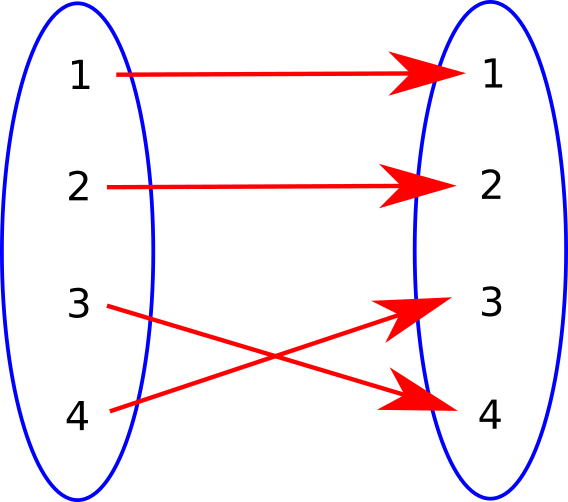
\includegraphics[width=0.5\linewidth]{transposition.png}
    \caption{Diagram of an example transposition.}
    \label{fig:transposition}
\end{figure}

\begin{defn}\index{Parity}
    Let $S_n$ denote the permutation group on $\{1,...,n\}$. We say that $\sigma \in S_n$ is an \textbf{even permutation} if it can be reproduced by an even number of transpositions. It is called an \textbf{odd permutation} if it can be reproduced by an odd number of transpositions.
    
    The \textbf{parity} $\sgn(\sigma)$ of a permutation is defined as follows.
    \[\sgn(\sigma) = \begin{cases}1 &\textsf{if } \sigma \textsf{ is even}\\
    -1 & \textsf{if } \sigma \textsf{ is odd}\end{cases}\]
\end{defn}
\begin{example}
    Any transposition is an odd permutation by definition.
\end{example}
\begin{example}
Let $n=3$. The permutation taking $(1,2,3)$ to $(2,3,1)$ can be achieved by swapping 1 and 3, then swapping 2 and 3. It is therefore an even permutation.
\end{example}
\begin{thm}[Decomposition of Permutations]
    Let $\sigma\in S_n$ be a permutation. Then there exists a finite list $\{\tau_1,...,\tau_N\}$ of transpositions so that $\sigma = \tau_1\circ...\circ \tau_N$. 

    In other words, if $T_n$ is the set of all transpositions in $S_n$ then $S_n = \langle T_n\rangle$.
\end{thm}
\begin{thm}
Parity satisfies the property that $\sgn(\sigma\circ\tau) = \sgn(\sigma)\sgn(\tau)$.
\end{thm}
\begin{cor}
    The parity of $\sigma$ can also be written as,
    \[\sgn(\sigma) = \begin{cases}1 &\textsf{if } \sigma \textsf{ is the product of an even number of transpositions}\\
    -1 & \textsf{if } \sigma \textsf{ is the product of an odd number of transpositions}\end{cases}\]
\end{cor}

\subsubsection{Group Homomorphisms}

\begin{defn}[Group Homomorphism]\index{Homomorphism!Group}
Let $G$ and $H$ be groups. Let $\phi : G \to H$ be a function.

Denote the group operation of $G$ by $f_G(g_1,g_2)$ and the group operation of $H$ by $f_H(h_1,h_2)$. We say $\phi$ is a \textbf{group homomorphism} (or just a \textbf{homomorphism}) if the following equation holds,
\[\phi(f_G(g_1,g_2)) = f_H(\phi(g_1),\phi(g_2))\]
\end{defn}
\begin{defn}[Kernel and Image]\index{Kernel!of Group Homomorphism}\index{Image!of Group Homomorphism}
    Let $\phi : G \to H$ be a group homomorphism.
    
    The image of $\phi$ is defined by $\image(\phi) = \{\phi(x): x\in G\}$. It is a subgroup of $H$.

    The kernel of $\phi$ is defined by $\ker(\phi) = \{x\in G: \phi(x)=e\}$. It is a subgroup of $G$.
\end{defn}
\begin{remark*}
    The kernel consists of anything getting mapped to the identity.

    The image is the set of all outputs.
\end{remark*}
\begin{thm}
    Consider the group $G = \{-1,1\}$, where the group operation is $f_G(a,b) = ab$. The map $\sgn : S_n \to G$ is a group homomorphism.
\end{thm}
\begin{proof}
    As we saw earlier, $\sgn(\sigma\circ\tau) = \sgn(\sigma)\sgn(\tau)$.
\end{proof}
\begin{defn}[Alternating Group]\index{Group!Alternating}
    The kernel of the map $\sgn : S_n \to G$ is denoted $\ker (\sgn) = A_n$, and is called the alternating group. It consists of all even permutations in $S_n$. It has order $|A_n| = n!/2$.
\end{defn}


\begin{defn}[Group Isomorphism]\index{Isomorphism!of Groups}
Let $G$ and $H$ be groups, and let $\phi : G \to H$ be a group homomorphism. If $\phi$ is bijective, we say it is a \textbf{group isomorphism}. Group isomorphism is an equivalence relation. 
\end{defn}

\begin{lemma}
    Suppose $\phi : G \to H$ is an injective group homomorphism. Then $\phi$ is an isomorphism between $G$ and $\image(\phi)$
\end{lemma}
\begin{proof}
    Let $y \in \image(\phi)$. Then by definition, there is an element $x$ of $G$ with $\phi(x)=y$. Therefore $\phi$ is surjective onto $\image(\phi)$. This completes the proof.
\end{proof}
\begin{lemma}
    Any two cyclic groups $G,H$ of order $|G|=|H|$ are isomorphic.
\end{lemma}
\begin{proof}
    Recall that $G = \langle g\rangle$ and $H = \langle h \rangle$.
    
    First we show that there is a unique homomorphism $\phi: G\to H$ so that $\phi(g) = h$. Suppose $\phi_1$ and $\phi_2$ are homomorphisms and that $\phi_1(g)=\phi_2(g)=h$. Then $\phi_1(g)^n = \phi_1(g^n)$ and $\phi_2(g)^n = \phi_2(g^n)$. So $\phi_1(g^n) = h^n=\phi_2(g^n)$ for all $n$. Since every element of $G$ is of the form $g^n$, we see that $\phi_1(x)=\phi_2(x)$ for all $x\in G$. Thus $\phi$ is unique.

    Now we show that it is surjective. Suppose $k \in H$. Then for some $|n|\leq |G|=|H|$, we have $k = h^n = \phi(g)^n = \phi(g^n)$.

    Finally, we show it is injective. Suppose $\phi(x) = e$. Then $\phi(x)k=k$ for all $k\in H$. So for some $n$ we have $\phi(x)h^n = h^n$, so $\phi(xg^n) = h^n$. Since $x \in G$ we have $x = g^q$ for some $q$, so $\phi(g^{q+n}) = h^n$. But $\phi(g^{q+n}) = h^{q+n}$. So we must have $q = a|G|$ for some $a \in \ZZ$. But $|G| = |H|$, so $g^{n+q} = g^n$ and $h^{n+q} = h^n$. This completes the proof.
\end{proof}
\begin{lemma}
    Let $G=\langle g\rangle$ be cyclic and finite. Then $g^{|G|} = e$. Furthermore, $g^{a+|G|k} = g^a$ for all $k\in\ZZ$.
\end{lemma}
\begin{remark*}
    This is why we call it a cyclic group.
\end{remark*}
\begin{proof}
Let $\ell$ be the smallest integer so that $g^\ell = e$. We can always write $k = \ell q+r$ for some remainder $r$, so $g^{\ell q+r} = g^{\ell q}g^r = e$. But $g^{\ell q} = (g^\ell)^q = e^q = e$. So $r=0$. Therefore if $g^k = e$ we must have $k = \ell q$ for some $q$.
We also have that for all $0< k\leq \ell-1$, $g^{-k} = g^a$ for some $a$. Since $g^\ell = e$, this means that $g^{\ell-k} = g^{-k}$. Since $0\leq \ell-k\leq \ell-1$ we have $a=\ell-k$. So $g^{-k} = g^{\ell-k}$.

Finally, observe that since $g^{-k} = g^{\ell - k}$ for all $k$, we have the following distinct elements of $G$: $\{e, g^1,g^2,...,g^{\ell-1}\}$. Thus $|G| = \ell$ and $g^{|G|} = e$ as required.
\end{proof}


\subsubsection{Quotient Groups and the First Isomorphism Theorem}
\begin{defn}[Coset of $h$] \index{Coset} Let $G$ be a group and let $h \in G$. Then the set $hG = \{hg : g \in G\}$ is called the right coset of $h$. The set $Gh = \{gh : g \in G\}$ is called the left coset of $h$.
\end{defn}
\begin{defn}[Coset of $H$] Let $G$ be a group and let $H$ be a subgroup of $G$. Then we define the left coset of $H$ to be $GH = \{gh : g\in G, h\in H\}$ and the right coset to be $HG = \{hg : g\in G, h \in H\}$.
\end{defn}
\begin{remark*}
    In general, we write $aHb = \{ahb : h \in H\}$. Similarly, $AHB=\{ahb : h \in H, a\in A, b\in B\}$.
\end{remark*}
\begin{defn}[Normal Subgroup]\index{Subgroup!Normal}
    Let $G$ be a group and let $H$ be a subgroup. Then we say $H$ is \textbf{normal} if $g^{-1} H g = H$ for all $g\in G$.
\end{defn}
\begin{thm}
    The following are equivalent.
    \begin{enumerate}
    \item {
    $H$ is normal.
    }
    \item {
    $g^{-1} H g = H$ for all $g \in G$.
    }
    \item {
    $gH = Hg$ for all $g \in G$.
    }
    \item {
    If $x \in aH$ and $y \in bH$ then $xy \in (ab)H$.
    }
    \item {
    For all $x,y \in G$ we have $(xH)(yH) = (xy)H$.
    }
    \item {
    There exists a group $K$ and a group homomorphism $\phi : G \to K$ with $\ker(\phi) = H$.
    }
    \end{enumerate}
\end{thm}
\begin{remark*}
    In other words, normal subgroups are just all the possible kernels of different maps out of $G$.
\end{remark*}
\begin{defn}[Quotient Group]\index{Group!Quotient}\index{Quotient!of Groups}
Let $G$ be a group and let $H$ be a normal subgroup of $G$. Then we define the quotient of $G$ by $H$ to be the collection of all cosets of $H$.
\begin{equation}G/H = \{gH : g \in G\}
\end{equation}
The set $G/H$ of all cosets of $H$ forms a group with the same operation as $G$, since $(aH)(bH) = (ab)H$.
\end{defn}
\begin{thm}[First Isomorphism Theorem/Noether's First Theorem]\index{Theorem!First Isomorphism Theorem (for Groups)}
    Let $\phi : G \to K$ be a surjective group homomorphism. Then $K$ is isomorphic to $G/\ker(\phi)$.
\end{thm}
\begin{proof}
    Let $g\ker(\phi) \in G/\ker(\phi)$. Then for any $gh \in g\ker(\phi)$ we have \[\phi(gh) = \phi(g)\phi(h) = \phi(g)e = \phi(g)\]

    Therefore, the map $\tilde{\phi} : G/\ker(\phi) \to K$, given by $\tilde{\phi}(g\ker(\phi)) = \phi(g)$, is well defined.
    
    As we can see, $\tilde{\phi}(g\ker(\phi)) = e$ if and only if $\phi(g) = e$, which means $\tilde{\phi}$ is injective. This completes the proof
\end{proof}
\begin{cor}
    $G/\ker(\phi)$ is isomorphic to $\image(\phi)$.
\end{cor}
\begin{thm}[Lagrange's Theorem]\index{Theorem!Lagrange's Theorem}
    If $H$ is a subgroup of $G$ then $|G|/|H|$ is an integer. In other words, the order of $H$ divides the order of $G$.
\end{thm}
\begin{proof}
    Consider the collection of left-cosets of $H$. 
    
    Suppose $x=gh_1 \in gH$. Then $x \in kH$ if and only if $x = kh_2$ for some $h_2\in H$, which means $gh_1 = kh_2$, or in other words, $gh_1h_2^{-1}=k$. 
    
    Since $h_1h_2^{-1} \in H$, it follows that $gH = kH$. Thus, two left cosets must be either equal or entirely disjoint. 
    
    Additionally, every left coset of $H$ is the same size since $|gH| = |H|$ for all $g$. Since there are an integer number of left cosets, it follows that $n|H|=|G|$, where $n$ is the number of left cosets of $H$.
    
    The number $n$ is called the \textbf{index}\index{Index!of Subgroup} of $H$ in $G$, and we often write it as $n = [G:H]$ so that $|H|[G:H] = |G|$.
\end{proof}

\subsubsection{Group Actions and Cayley's Theorem}
\begin{defn}[Group Action] \index{Group!Action} Let $S$ be a set and let $G$ be a group. Then a (left) \textbf{group action} is a function $A : G\times S \to S$, with the following properties:
\begin{enumerate}
\item {
Compatibility: $A(gh,s) = A(g,A(h,s))$.
}
\item {
Identity: $A(e,s) = s$.
}
\end{enumerate}
Notationally, we often write $A(g,s) = g\cdot s$ as long as this can't be confused with some other operation.
\end{defn}
\begin{defn}[Transitive Action]
\index{Group!Action!Transitive}
    A group action $A: G\times S \to S$ is called transitive, if for all $x,y \in S$ there exists some $g$ with $A(g,x) = y$.
\end{defn}
\begin{thm}[Cayley's Theorem] Any finite group $G$ is isomorphic to a subgroup $H$ of $S_n$, for some $n \in \NN$.
\end{thm}
\begin{proof}
Let $k = |G|$ be the order of $G$. Consider the left group-action of $G$ on itself, $A : G \times G\to G$ given by $A(g,h) = gh$. 

We can see that the action is invertible, since $A(g^{-1},g) =A(g,g^{-1}) = e$. 

We can also see that $A$ is transitive, since if $x,y \in G$ we have $x^{-1}y\in G$, so we can simply take $A(x,x^{-1}y) = y$. 

Therefore, for each $g \in G$ we have an invertible function $A_g : G \to G$ defined by $A_g(h) = A(g,h)$.

Since $|G|=k$, each function $A_g$ simply permutes the $k$ elements of $G$ around. Therefore we have a mapping $\tilde{A} : G \to S_k$ given by $\tilde{A}(g) = A_g$. 

We also have \[\tilde{A}(g)\tilde{A}(h)(x) = ghx = \tilde{A}(gh)(x)\]

Therefore $\tilde{A}$ is a homomorphism, and $\image(\tilde{A})$ is a subgroup of $S_k$. 

Since $\tilde{A}(g)(h) = gh = e$ iff $g = h^{-1}$, it also follows that $\tilde{A}$ is injective, and is hence an isomorphism between $G$ and $\image(\tilde{A})$ as required.
\end{proof}

\subsection{Rings}
We will only review a few definitions for rings.
\begin{defn}[Ring]\index{Ring}
Let $R$ be a commutative group. That is, there exists an operation $+ : R \times R \to R$ which is associative, commutative, invertible, and has an identity $0$. Suppose there is another operation, $\cdot : R\times R \to R$, which satisfies the following properties,
\begin{enumerate}
\item {Associative: $a\cdot(b\cdot c) = (a\cdot b)\cdot c$}
\item {Distributive: $a\cdot(b+c)=a\cdot b + a\cdot c$ and $(b+c)\cdot a = b\cdot a + c\cdot a$}
\item {Identity: There exists $1\in R$ so that $1\cdot a = a\cdot 1 = a$ for all $a$.}
\end{enumerate}
Then we say that the data $(R,+,\cdot)$ forms a \textbf{ring}. For short, we just call $R$ a ring and we usually write $a\cdot b = ab$.
\end{defn}
\begin{defn}[Ideal]
    A \textbf{ring ideal} is a subset $I\subseteq R$ with the following properties.
    \begin{enumerate}
    \item {$I$ is a subgroup of $R$ with respect to addition.}
    \item {For all $a \in R$, $b\in I$, we have $ab \in I$}
    \end{enumerate}
\end{defn}
\begin{defn}[Generating Set of Ideal]
    The \textbf{ideal generated by} a subset $S$ is defined to be the smallest ideal containing $S$. We denote it $(S)$. For $S=\{a_1,...,a_n\}$ we let $(S) = (a_1,...,a_n)$.  
\end{defn}
\begin{example}
    $\ZZ,\QQ,\RR,\CC$ are all rings.
\end{example}
\begin{example}
    Let $R$ be a ring. Let $R[x]$ denote the set of all polynomials whose coefficients are elements of $R$. Then $R[x]$ is also a ring.
\end{example}
\begin{defn}[Coset of Ideal]\index{Coset!Ideal}
    Let $I$ be an ideal in $R$. Then we define the cosets of $I$ to be the sets of the form $a+I$, $a\in R$. This is exactly the same as the construction for subgroups.
\end{defn}
\begin{defn}[Quotient Ring]
    Let $I$ be an ideal in $R$. Then we define $R/I$ to be the set of all cosets of $I$. This forms a ring.
\end{defn}
\begin{example}
    Let $R = \RR$ and consider the set of all real polynomials $\RR[x]$. Observe that $x^2 +1$ has no roots in $\RR$, which means it can not be factored. Let $(x^2+1)$ be the ideal generated by this polynomial.
    
    The quotient, $\RR[x]/(x^2+1)$, consists of all objects of the form $f(x)+I$, and two polynomials in $\RR[x]/(x^2+1)$ are said to be equivalent if they differ by a polynomial of the form $h(x)(x^2+1)$.

    Let $\phi : \RR[x]/(x^2+1)\to \CC$ be defined as follows. $\phi([f]) = f(i)$. Observe that since $i^2-1=0$, this does not depend on the choice of representative for $[f]=f+I$. Additionally, \[\phi([f]+[g])= f(i)+g(i) = \phi([f])+\phi([g])\]
    and \[\phi([fg]) = f(i)g(i) = \phi([f])\phi([g])\]
    So $\phi$ is a ring homomorphism.

    Suppose $f$ is a degree $k$ polynomial. Then it is of the form $f(x) = a_k x^k + ... + a_2 x^2 + a_1 x + a_0$. Then we can rearrange this as follows. 
    \begin{align*}f(x) +I&= a_kx^{k-2}(x^2 -1 +1) + ... + a_2(x^2-1+1) + a_1 x + a_0 + I\\
    &= (a_k x^{k-2}+...+a_2)(x^2+1) - (a_k x^{k-2} + ... + a_2) + a_1 x + a_0+I\\
    &=  - (a_k x^{k-2} + ... + a_2) + a_1 x + a_0 + I\\
    &= -(a_k x^{k-4}(x^2-1+1)+...+a_4(x^2-1+1)) + (a_1-a_3)x+(a_0-a_2) + I\\
    &=...\\
    &= (a_1\pm a_3\pm ...\pm a_{p})x+(a_0\pm a_2\pm ...\pm a_q) + I
    \end{align*}   
    Where $p$ is the largest even number less than or equal to $k$, and $q$ is the largest odd number less than or equal to $k$. Therefore we see that for any $f +I\in \RR[x]/(x^2+1)$ we can reduce $f$ to a first order polynomial. Since the coefficients $a_i$ can be chosen however we want, this means that for any $a,b\in \RR$ there is a polynomial $f$ so that $\phi([f]) = a+bi$. So $\phi$ is surjective.

    Finally, let $\phi^{-1}(a+bi) = a+bx$. Then since any $[f]$ has a first order representative, $\phi^{-1}$ is surjective. 
    
    Therefore $\phi$ is a ring isomorphism.

    Thus we have shown that $\CC$ is isomorphic to $\RR[x]/(x^2+1)$.
\end{example}
\begin{remark*}
    This is one way of defining the complex numbers. In this course we will study another definition in depth, called the Cayley-Dickson construction, which defines $\CC$ as a vector algebra over $\RR$.
\end{remark*}
\begin{defn}[Field (alternative definition)]\index{Field!Definition using rings}
    Let $R$ be a ring. Then if for all $0\neq a \in R$ there exists $a^{-1} \in R$ so that $a\cdot a^{-1} = a^{-1} \cdot a=1$, we say $R$ is a \textbf{field}.
\end{defn}

\section{Appendix II: Linear Algebra}
\subsection{Vector Spaces}
\subsubsection{Basic Definitions}
This content can all be found in standard books \cite{Axler2015-in,Roman2008-rh}
\begin{defn}[Vector Space]\index{Vector!Space}
A vector space is defined by the data of a set $V$, along with a field $\FF$ called the set of scalars. The set $V$ is equipped with a notion of addition. That is, for any two vectors $v$ and $w$ in $V$, we can add them to produce a third vector $v+w$.

In addition to this notion of vector addition, we also have a notion of scalar multiplication. That is, the vectors $v \in V$ can be scaled by an element $a$ of $\FF$ to produce a new vector $av \in V$. 

These two operations must follow the vector space axioms.
\begin{enumerate}
\item {
Commutativity: if $v,w \in V$ then $v + w = w+v$
}
\item {
Associativity: if $a,b \in \FF$ and $v \in V$, we have $a(bv) = (ab)v$
}
\item {
Distributivity: if $a \in \FF$ and $v,w \in V$ we have $a(v+w)=av+aw$.
}
\end{enumerate}
\end{defn}
\begin{remark*}
    If we replace the field $\FF$ in the above definition with an arbitrary ring $R$, then we get something called a \textbf{module} instead of a vector space.\index{Module}
\end{remark*}
\begin{defn}[Linear Subspace]\index{Linear!Subspace} Let $V$ be a vector space. A linear subspace is a subset $U \subseteq V$ which is also a vector space, with the same underlying field, scalar multiplication, and addition operations.
\end{defn}

\begin{example}
There are a great many examples of vector spaces. I will list just a few kinds of vector spaces we will encounter.

\begin{enumerate}
\item {
Vector spaces of the form $\FF^n$, such as $\RR^n$ or $\CC^n$. These are formed by taking the Cartesian product of a field with itself $n$ times. The addition operation is defined by $(a_1,...,a_n) + (b_1,...,b_n) = (a_1+b_1,...,a_n+b_n)$.
}
\item {
Vector spaces of functions. For example, $C_0(\RR)$ denotes the set of continuous functions from $\RR$ to $\RR$. This set is a vector space since we know that two continuous functions can be added to produce a third continuous function. They can also be scaled by real numbers, and the result will still be continuous.
}
\item {
Vector spaces formed by combining two vector spaces in some nice way. For example, if $V$ and $W$ are vector spaces we could form the direct sum of $V$ and $W$. The direct sum, denoted $V \oplus W$, is the set of all linear combinations of elements of $V$ and $W$.
}
\end{enumerate}
\end{example}
\begin{defn}[Span]\index{Span}
Let $V$ be a vector space over $\FF$. Let $v_1,...,v_n$ be a collection of vectors in $V$. We define
\begin{equation}
    \Span(\{v_1,...,v_n\}) = \left\{\sum_{i=1}^n a_i v_i : a_i \in \FF\right\}
\end{equation}
\end{defn}

\begin{defn}[Direct Sum]\index{Direct!Sum} Let $V$ and $W$ be vector spaces. The direct sum of $V$ and $W$ is the vector space 
\begin{equation}V\oplus W = \{v+w: v \in V, w \in W\} = \textsf{span}(V\cup W)\end{equation}
For a list of $k$ vector spaces $V_1,...,V_k$ we write,
\begin{equation}
    V_1\oplus...\oplus V_k = \bigoplus_{i=1}^k V_i
\end{equation}
\end{defn}

\begin{example}
    Let $V$ and $W$ be vector spaces. Then their Cartesian product $V \times W$ is a vector space.
\end{example}
\begin{proof}
    Consider $a \in \FF$, $(v_1,w_1) \in V \times W$ and $(v_2,w_2)\in V\times W$. Then we define addition and scalar multiplication according to the rule $(v_1,w_1)+a(v_2,w_2) = (v_1+av_2,w_1+aw_2)$. As we can see, this is an element of $V \times W$. We can verify each of the vector space axioms as well:
    \begin{enumerate}
    \item {
    $(v_1,w_1) + (v_2,w_2) = (v_1+v_2,w_1+w_2) = (v_2+v_1,w_2+w_1) = (v_2,w_2)+(v_1,w_1)$
    }
    \item {
    $a(b(v,w)) = a(bv,bw) = ((ab)v,(ab)w) = (ab)(v,w)$
    }
    \item {
    \begin{align*}
    a((v_1,w_1)+(v_2,w_2)) &= a(v_1+v_2,w_1+w_2)\\
    &= (av_1+av_2,aw_1+aw_2)\\
    &= (av_1,aw_1) + (aw_1,aw_2)\\
    &= a(v_1,w_1)+a(v_2,w_2)
    \end{align*}
    }
    \end{enumerate}
\end{proof}

An important property of vectors is linear independence.
\begin{defn}[Linearly Independent]\index{Linear!Independence}
    Let $V$ be a vector space over $\FF$. Then a collection of $n$ nonzero vectors $v_1,...,v_n$ are called linearly independent if the following property holds.
    
    Whenever $a_1,...,a_n \in \FF$ then $a_1v_1+...+a_nv_n = 0$ if and only if $a_1=...=a_n=0$. 
\end{defn}
\begin{example}
    Consider $V = \RR^3$. Then the vectors $e_1=(1,0,0)$, $e_2=(0,1,0)$, and $e_3=(0,0,1)$ are linearly independent.
\end{example}
\begin{proof}
Suppose $a_1e_1+a_2e_2+a_3e_3=0$. Observe that $a_1e_1+a_2e_2+a_3e_3 = (a_1,a_2,a_3)$. Since $(a_1,a_2,a_3)=(0,0,0)$, we must have $a_1=0,a_2=0,a_3=0$. Therefore $e_1,e_2,e_3$ must be linearly independent.
\end{proof}

\begin{defn}[Dimension]\index{Vector Space!Dimension}
    Let $V$ be a vector space over $\FF$. The dimension $\dim V$ is the largest possible number $n$ with the property that there exists a set of linearly independent vectors of size $n$.
\end{defn}

\begin{defn}[Basis]
    Let $V$ be a vector space and let $B$ be a set of linearly independent vectors such that $V = \textsf{span}(B)$. We say that $B$ is a basis for $V$.
\end{defn}
\begin{thm}
    Let $V$ be a finite dimensional vector space. Then every basis for $V$ has $\dim V$ elements. Furthermore, if $B$ is a linearly independent subset of $V$ of size $\dim V$, then $B$ is a basis for $V$.
\end{thm}
\begin{thm}
    Let $V$ be a vector space and let $W$ be a subspace of $V$. Then if $\dim W = \dim V$ we have $W=V$.
\end{thm}
\begin{proof}
    Let $\{e_1,...,e_n\}$ be a basis for $W$. Then if $V$ is $n$-dimensional, $e_1,...,e_n$ must also be a basis for $V$. Therefore $V = \textsf{span}\{e_1,...,e_n\} = W$.
\end{proof}

\begin{thm}
    Let $V$ be a vector space and let $U,W$ be subspaces of $V$. Then their intersection $U\cap W$ is a vector space, and $U\cap W = \{0\}$ if and only if $U$ and $W$ are linearly independent subspaces.
\end{thm}
\begin{remark*}
    The union of two vector subspaces is \textbf{not necessarily} a vector space.
\end{remark*}
A very special kind of vector space merits its own definition. Vector algebras are vector spaces with a notion of vector multiplication. 

\begin{defn}[Algebra]\index{Vector!Algebra}\index{Algebra} An \textbf{algebra} is a vector space equipped with a notion of vector multiplication. That is, for any two vectors $v,w \in V$ we can multiply them to produce a third vector, $v \times w$. This operation is not required to be commutative, but must satisfy the following axioms:
\begin{enumerate}
\item {
Distributivity: for all $u,v,w \in V$ we have $u\times(v+w) = u\times v + u\times w$
}
\item {
Scaling rule: for all $a \in \FF$, and $u,v\in V$, we have $a(v\times w) = (av) \times w = v\times (aw)$
}
\end{enumerate}
If in addition the algebra satisfies $u\times (v\times w) = (u\times v) \times w$, we say $A$ is an \textbf{associative algebra}.
\end{defn}
\begin{remark*}
    We call this type of vector space an ``algebra" because it has all of the tools required to do algebra: multiplication and addition.
\end{remark*}
\begin{defn}
    Let $V$ be an algebra and let $W$ be a vector subspace of $V$. Then $W$ is said to be a subalgebra of $V$ if for all $a,b\in W$ we have $ab\in W$ and $ba \in W$.\index{Subalgebra}\index{Algebra!Subalgebra}
\end{defn}
\begin{example}[Examples of Algebras]
The following are a few examples of algebras.
\begin{enumerate}
\item {
Matrix algebras.\index{Matrix!Algebra} The set $M_{nn}(\RR)$ of n by n matrices forms an algebra, where the "vector multiplication" is really just matrix multiplication. Note that this is not commutative! Many algebras are isomorphic to matrix algebras (this isomorphism is called a faithful representation).
}
\item {
The set of continuous functions, $C_0(\RR)$, has the property that if $f$ and $g$ are continuous, then their composition, $f \circ g$, is continuous. Therefore $C_0(\RR)$ is a vector algebra, where the ``multiplication" is composition. Note that this is not commutative! $f\circ g \neq g \circ f$.
}
\item {
The spaces $\RR^1$, $\RR^3$, and $\RR^7$ all have a special operation defined on them called the cross product. This is denoted $v \times w$, and it also has the property that $v \times w = -w \times v$. Therefore, $\RR, \RR^3$ and $\RR^7$ are algebras when equipped with the cross product.
}
\end{enumerate}
\end{example}
\begin{example}[Non-example of an Algebra]
The set $\GL_n(\RR)$ of invertible $n\times n$ matrices is \textbf{not} an algebra since not every linear combination of invertible matrices is invertible. It is closed under matrix multiplication but not addition. For instance, if $M\in \GL_n(\RR)$ then $M-M=0\not\in \GL_n(\RR)$ since the zero matrix is not invertible.

\end{example}
\subsubsection{Maps Between Vector Spaces}

The vast majority of the time we are only going to be interested in maps between vector spaces which don't interfere with the laws of arithmetic. That is, you should be able to scalar multiply or add vectors before applying a map, and get the same thing if you were to apply the map and then add/scale the result.

Maps with this property are called homomorphisms, or "structure preserving maps". In the case where the operations we would like to preserve are vector space operations, these maps are what we call "linear".

\begin{defn}[Linear Map] \index{Linear!Map} Let $V$ and $W$ be vector spaces over $\FF$. Then a map $T : V \to W$ is called linear if for all $a \in \FF$ and $u,v \in V$, we have $T(au+v) = aT(u)+T(v)$. If $W=V$ we say $T$ is a \textbf{linear operator}.\index{Linear!Operator}
\end{defn}
\begin{defn}[Space of Linear Maps]
    The set of all linear maps from $V$ to $W$ is denoted $L(V,W)$. It forms a vector space. For simplicity we often write $L(V,V)=L(V)$ when the domain and range are the same.
\end{defn}

\begin{remark*}
Why are these maps called linear? The answer is that if $L \subseteq V$ is a line through the origin in $V$ (that is, a one-dimensional subspace of $V$), then if you apply a linear map $T$ to every point in $L$, the result $T(L)$ is also a line through the origin in $W$. Therefore, linear maps are exactly the functions which send lines through the origin to lines through the origin.
\end{remark*}
\begin{defn}[Isomorphism]\index{Isomorphism}
    Let $T : V \to W$ be a linear map. If $T$ is also bijective, then $T$ is an \textbf{isomorphism}.
\end{defn}
\begin{remark*}
    An isomorphism is a way to make two vector spaces equivalent. If one completes some calculation in a vector space $V$, and $V$ is isomorphic to some other space $W$, then the same calculation can easily be translated to $W$.
\end{remark*}
\begin{defn}
    Let $V$ be a vector space. An isomorphism from $V$ to itself is called a \textbf{endomorphism}. The set of endomorphisms is a vector space called $\End(V)$, and it is a subspace of $L(V)$.\index{Endomorphism}
\end{defn}

\begin{defn}[Fundamental Subspaces] Let $V,W$ be vector spaces and let $T : V \to W$ be a linear map. The fundamental 
vector subspaces associated to $T$ are the following sets.
\begin{enumerate}
\item {\index{Image!of Linear Map}
The image of $T$ (also known as the range). Defined as \[\textsf{image}(T) = \{T(v) : v \in V\}\]
This is a subspace of $W$. The \textbf{rank} of $T$ is defined by $\Rank(T) = \dim(\image(T))$. This is an \textit{invariant} of $T$. \index{Invariant!Rank of a Linear Map}
}
\item {\index{Kernel!of Linear Map}
The kernel of $T$ (also known as the null-space). Defined as \[\textsf{ker}(T) = \{v \in V : T(v)=0\}\]
This is a subspace of $V$. It contains all vectors which are mapped to zero by $T$. The \textbf{nullity} of $T$ is the dimension of $\ker T$.
}
\end{enumerate}
\end{defn}
\begin{thm}[Rank-Nullity Theorem]
\index{Theorem!Rank-Nullity Theorem}Let $T : V \to W$ be a linear map. Then 
\begin{equation}\dim \image T = \dim W - \dim \ker T\end{equation}
\end{thm}
\begin{thm}
    Let $T : V \to W$ be a linear map. Then $T$ is injective if and only if $\ker T = \{0\}$.
\end{thm}
\begin{proof}
First suppose $T$ is injective. Now let $v_1,v_2 \in \ker(T)$. This means that $T(v_1)=T(v_2)=0$. 

But then since $T$ is injective, $v_1=v_2$. Therefore every vector in $\ker(T)$ is equal to every other vector in $\ker(T)$.

The only way for this to be possible is for $\ker(T)$ to contain exactly one vector. 

Since $T(0)=0$, this vector must be the zero vector. So $\ker(T) = \{0\}$.

Now suppose $\ker(T)=\{0\}$. Then let $v_1,v_2 \in V$ and suppose $T(v_1)=T(v_2)$. 

So $T(v_1-v_2)=0$, which means $v_1-v_2 \in \ker(T)$. 

But the only thing in $\ker(T)$ is the zero vector, so $v_1=v_2$. Therefore $T$ is injective.
\end{proof}
\begin{thm}
Let $T : V \to W$ be an injective linear map. Then $T$ is an isomorphism if $\dim W = \dim V$.
\end{thm}
\begin{proof}
Suppose $\dim W = \dim V$. Let $B=\{v_1,...,v_n\}$ be a basis for $V$. Then let $T(B) = \{T(v_1),...,T(v_n)\}$. Observe that since $T$ is injective, $T(v_i)-T(v_j)$ if and only if $v_i=v_j$. 

Now, we would like to show that $T(B)$ is a basis for $W$. We can do this by showing that it is linearly independent. 

Consider any set $a_1,...,a_n \in \FF$. Then $a_1T(v_1)+...+a_nT(v_n) = 0$ if and only if $T(a_1v_1+...+a_nv_n)=0$. 

But since $T$ is injective, this means
\[a_1v_1+...+a_nv_n=0\]
Since $v_1,...,v_n$ are linearly independent we conclude that \[a_1=...=a_n=0\] 

Therefore $T(v_1),...,T(v_n)$ are linearly independent. Since $\dim W = \dim V$, we conclude that $T(B)$ is a basis for $W$. 

Finally, since $T(B)$ is a basis for $W$, that means for any $w \in W$ we have 
\[w = \sum_{i=1}^n w_i T(v_i) = T\left(\sum_{i=1}^n w_i v_i\right)\] 

So for all $w \in W$ there exists $v$ so that $T(v)=w$. So $T$ is surjective, and hence $T$ is an isomorphism.
\end{proof}

\begin{cor}
    Let $T : V \to W$ be a linear map and let $B$ be any basis for $V$. Then if $T(B)$ is a basis for $W$, it follows that $T$ is surjective.
\end{cor}
\begin{proof}
    Exercise. Hint: See the proof of the previous theorem.
\end{proof}


\begin{thm}[Extension by Linearity]\index{Extension by Linearity}\index{Linear!Extension}
Let $V,W$ be two vector spaces and let $B = \{v_1,...,v_n\}$ be a basis for $V$. Then if we specify some desired outputs $w_1,...,w_n\in W$, there is a \textbf{unique} linear map $T : V \to W$ which satisfies $T(v_i)=w_i$ for each $i=1,...,n$. Additionally, $\textsf{image}(T) = \textsf{span}\{w_1,...,w_n\}$.
\end{thm}
\begin{proof}
If we require that $T$ is linear, and that $T(v_i) = w_i$ for each $i=1,...,n$ then for any $v \in V$ we get
\begin{align*}
    T(v) &= T\left(\sum_{i=1}^n a_i v_i\right)\\
    &= \sum_{i=1}^n a_i T(v_i)\\
    &= \sum_{i=1}^n a_i w_i
\end{align*}
Therefore we only need to know $T(v_i)$ for each $i=1,...,n$ in order to \textbf{completely} specify $T(v)$ for all $v\in V$.
\end{proof}

When we do calculations, we don't always want to have an abstract definition for our linear map. For numerical calculations it is much more convenient to put the linear map in matrix form. To do this, we need a basis.

\begin{defn}The set of all $n\times n$ matrices with entries in a field $\FF$ will be denoted $M_{nn}(\FF)$. Any matrix is also a linear map from $\FF^n$ to $\FF^n$.    
\end{defn}
\begin{defn}[Matrix of a Linear Map]\index{Matrix!of a Linear Map} Let $V,W$ be finite dimensional vector spaces and let $B = \{e_1,...,e_n\}$ be a basis for $V$ and $C=\{f_1,...,f_n\}$ be a basis for $W$. Let $T : V \to W$ be a linear map. Then the matrix $[T]_{CB}$ is defined by the following formula
\[[T]_{CB}[v]_B = [T(v)]_C \qquad \textsf{for all }v\in V\]
Where $[v]_B = (v_1,...,v_n)$ is the $n\times 1$ matrix of coefficients defined by $v = \sum_{i=1}^n v_i e_i$. In other words, we can write
\[[T]_{CB} = \sum_{i=1}^n\sum_{j=1}^n T_{ij} v_i f_j\]
Where $T_{ij}$ are the entries of the matrix $[T]_{CB}$.
In an upcoming section, we will employ Einstein notation to make things like this less tedious to read and write.
\end{defn}

\begin{thm}
    Let $T : V \to V$ be a linear map, and let $[T]_{BB} \in M_{nn}(\FF)$ be the matrix for $T$ in some basis. The following are equivalent.
    \begin{enumerate}
    \item {$T$ is invertible}
    \item {The columns of $[T]$ are linearly independent}
    \item {The only solution to the equation $T(v) = 0$ is $v=0$ }
    \end{enumerate}
\end{thm}

A very useful computational tool when dealing with finite dimensional linear maps is the determinant, which allows us to easily determine whether a given matrix is invertible.
\begin{defn}[Determinant]\index{Determinant}
Let $M$ be an $n\times n$ matrix with entries $M_{ij}$, $i,j=1,...,n$. The determinant of $M$ is given by the following formula
\[\det M = \sum_{\sigma \in S_n} \left(\sgn\sigma \prod_{i=1}^n M_{\sigma(i)i}\right)\]
This formula is called the \textbf{Laplace expansion} of the determinant.\index{Laplace expansion}
\end{defn}
\begin{thm}The function $\det : M_{nn}(\FF) \to \FF$ is the unique function satisfying the following properties:
\begin{enumerate}
\item {
For all $A,B\in M_{nn}(\FF)$ we have $\det (AB) = \det A \det B$. 

If $A$ is invertible we therefore have $\det (A^{-1}) = (\det A)^{-1}$
}
\item {
Let $A = [a_1,a_2,...,a_n]$ be the matrix formed from the columns $a_1,...,a_n\in \FF^n$. Then 
\[\det [...,a_i,...,a_j,...] = - \det [...,a_j,...,a_i,...]\]
That is, swapping two columns introduces a minus sign to the result.
}
\item {
For any $\lambda \in \FF, v\in \FF^n, w\in \FF^n$ we have
\[\det [...,\lambda v + w,...] = \lambda^n \det [...,v,...] + \det [...,w,...]\]
That is, $\det$ is homogenous of degree $n$ in each column.
}
\end{enumerate}
\end{thm}
\begin{proof}
    The first point that $\det (AB) = \det A \det B$ is a bit difficult to prove. However, the other two points follow straightforwardly from the definition of the determinant above. We will not show that the determinant is the unique map satisfying these properties.
\end{proof}
\begin{thm}
    $\det A^T = \det A$.
\end{thm}
\begin{thm} Let $\FF$ be a field of characteristic $\textsf{char}(\FF)\neq 2$. 
A matrix $A \in M_{nn}(\FF)$ is invertible if and only if $\det A \neq 0$.
\end{thm}

\begin{thm}Let $V$ be a vector space and let $T : V \to V$ be a linear map. Let $B$ and $C$ be two bases for $V$. Then $\det [T]_B = \det [T]_C$. We therefore simply write $\det T$ for the determinant of a linear map, since it does not matter what bases we use to compute it. That is, $\det T$ is an \textit{invariant} of $T$\index{Invariant!Determinant of Linear Map}.
\end{thm}
\begin{proof}
Recall that there exists an invertible matrix $P_{BC}$ so that $[T]_{B} = P_{BC} [T]_{C} P_{BC}^{-1}$. Therefore 
\begin{align*}\det [T]_B &= \det(P_{BC} [T]_{C} P_{BC}^{-1} ) \\&= \det (P_{BC}) \det [T]_{C} \det( P_{BC}^{-1}) \\
&= \frac{\det (P_{BC})}{\det (P_{BC})} \det [T]_{C} \\
&= \det [T]_C
\end{align*}
as required.
\end{proof}

\subsubsection{Inner Products and Eigenvectors}
\begin{defn}[Eigenvector]\index{Eigenvector}
    Let $V$ be a vector space over $\FF$ and let $T : V \to V$ be a linear map. Then a vector $v \in V$ is said to be an \textbf{eigenvector} of $T$ if $T(v) = \lambda v$ for some $\lambda \in \FF$. The value $\lambda$ is said to be an \textbf{eigenvalue} of $T$.
\end{defn}
\begin{remark*}
    Observe that $T(v) = \lambda v$ iff $T(v)-\lambda v = 0$ iff $(T-\lambda \One)v = 0$. This equation only has a nonzero solution if $\det (T-\lambda\One)=0$. The expression $\chi(\lambda)=\det(T-\lambda\One)$ is a polynomial of degree $n$, and is called the \textbf{characteristic polynomial}. 
\end{remark*}

\begin{defn}[Characteristic Polynomial]\index{Characteristic Polynomial}
The \textbf{characteristic polynomial} of $T$ is $\chi(\lambda) = \det(T-\lambda \One)$. It is an \textit{invariant} of $T$.\index{Invariant!Characteristic Polynomial}
\end{defn}

Suppose we are working over $\FF=\CC$. Then there are guaranteed to be $n$ roots of $\chi(\lambda)$ up to multiplicity.

\begin{defn}[Algebraic Multiplicity]
    \index{Multiplicity!Algebraic}
    Let $\FF=\CC$, let $T : V\to V$, $\dim V = n$, and let $\chi(\lambda)$ be the characteristic polynomial of $T$. Let $\lambda_1,...,\lambda_k$ be the roots of $\lambda$. Then there are some integers $a_i,i=1,...,k$ so that $\chi(\lambda) = \prod_{i=1}^k (\lambda-\lambda_i)^{a_i}$ and $\sum_{i=1}^k a_i = n$. The integer $a_i$ is called the \textbf{algebraic multiplicity} of the eigenvalue $\lambda_i$.
\end{defn}
For a given eigenvalue $\lambda_i$ of $T$, the solutions to $T(v)=\lambda_i v$ form a vector space of dimension $\dim \ker(T-\lambda_i\One)$.
\begin{defn}[Geometric Multiplicity] \index{Multiplicity!Geometric}Let $\lambda_i$ be an eigenvalue of $T$. Then $g_i=\dim \ker(T-\lambda_i\One)$ is called the \textbf{geometric multiplicity} of $\lambda_i$.
\end{defn}
In practice, we write $T-\lambda_i\One$ in some basis and solve the resulting system of equations. There are some useful theoretical results that help us bound the number of linearly independent sets of solutions.
\begin{thm}
    Let $T$ be a linear map and let $\lambda_i,g_i$, $i=1,...,k$ be the eigenvalues and their algebraic multiplicities. Then $1\leq \dim \ker (T-\lambda_i \One) \leq g_i$.
\end{thm}
\begin{defn}[Inner Product]\index{Product!Inner}
Let $V$ be a complex vector space. Then an \textbf{inner product} on $V$ is a bilinear function $g : V \times V \to \CC$ with the following properties
\begin{enumerate}
\item {
$g(v,v)\geq 0$, with $g(v,v)=0$ iff $v=0$
}
\item {
$g(v,w)=\overline{g(w,v)}$
}
\end{enumerate}
\end{defn}
\begin{defn}[Matrix of Inner Product]\index{Matrix!of Inner Product}
    Let $\{e_1,...,e_n\}$ be a basis for $V$. Then set $g_{ij} = g(e_i,e_j)$. The matrix whose entries are $g_{ij}$ is denoted $[g]_B$. We have $\innprod{v,w} = \overline{[v]}^T_B [g]_B [w]_B$ for any basis $B$. Additionally, if $P_{B\tilde{B}}$ is a change of basis matrix, then $[g]_{\tilde{B}} = P_{B\tilde{B}}^T [g]_B P_{B\tilde{B}}$.
\end{defn}
\begin{defn}[Orthonormal Basis]\index{Orthonormal Basis}
    Let $B=\{e_1,...,e_n\}$ be a basis for $V$ and suppose $g(e_i,e_j)=\delta_{ij}$. Then $B$ is said to be an \textbf{orthonormal basis}.
\end{defn}
\begin{thm}[Gram-Schmidt Procedure] Let $g$ be an inner product on $V$. Then there exists an orthonormal basis for $V$.\index{Gram-Schmidt Procedure}
\end{thm}
\begin{proof}
    Let $B=\{e_1,...,e_n\}$ be any basis for $V$. Then set,
    \begin{align*}
        b_1 &= \frac{e_1}{\sqrt{g(e_1,e_1)}}\\
        b_2 &= \frac{e_2}{\sqrt{g(e_2,e_2)}} - g(e_1,e_2)b_1\\
        \vdots\\
        b_k &= \frac{e_k}{\sqrt{g(e_k,e_k)}} - \sum_{i=1}^k g(e_i,e_k)b_i
    \end{align*}
    The vectors $b_1,...,b_n$ are linearly independent and orthonormal and are a basis for $V$. The remainder of the proof is left as an exercise.
\end{proof}
\begin{defn}[Hermitian Transpose]
Let $T : \CC^n \to\CC^n$ be a linear map and let $\langle v,w\rangle$ denote the standard complex inner product. Then the \textbf{Hermitian transpose} $T^\dagger$ is the map defined by $\langle T(v),w\rangle = \langle v,T^\dagger(W)\rangle$ for all $v,w\in \CC^n$.
\end{defn}
\begin{defn}[Hermitian Adjoint] In general, if $V$ is any complex vector space with a complex inner product, we can define the \textbf{Hermitian adjoint} by the formula $\langle T(v),w\rangle = \langle v,T^\dagger(W)\rangle$. Note that $[T^\dagger]_{BB}$ is not always the same as $\overline{[T]}_{BB}^T$.
\end{defn}

\begin{defn}[Normal Operator]\index{Matrix!Normal}\index{Operator!Normal} Let $V$ be a complex vector space. A \textbf{normal operator} $A: V\to V$ is a linear map with the property that $AA^\dagger = A^\dagger A$.
\end{defn}
\begin{defn}[Symmetric Matrix]\index{Symmetric!Matrix}\index{Matrix!Symmetric} A \textbf{symmetric matrix} $A$ is a real or complex matrix with the property that $A^T = A$. Symmetric matrices are normal.
\end{defn}
\begin{example}\index{Orthogonal!Matrix}\index{Matrix!Orthogonal}
Consider $\FF = \RR$ with the standard inner product $\innprod{v,w} = v^T w$. 
Let $A\in M_{nn}(\RR)$ and suppose $A^T A = \One$. Then the columns of $A$ are all orthonormal with respect to the standard inner product on $\RR^n$. We therefore say that $A$ is an \textbf{orthogonal matrix} if $A^T A = \One$. Orthogonal matrices are normal and invertible. 
\end{example}
\begin{defn}[Unitary Operator]
A linear map $T: \CC^n \to \CC^n$ is said to be \textbf{unitary} if $A^\dagger A = \One$. Unitary operators are normal and invertible.
\end{defn}
\begin{defn}[Hermitian Matrix]
An operator $T :\CC^n\to \CC^n$ is called \textbf{Hermitian} if $T = T^\dagger$. Hermitian operators are normal.
\end{defn}

\begin{defn}[Diagonalizable] Let $V$ be a vector space. A linear map $T:V\to V$ is said to be diagonalizable if there exists a basis $B$ where $[T]_{BB}$ is diagonal.
\end{defn}
\begin{thm}
    Let $T : V \to V$ be a linear map. Then $T$ is diagonalizable if and only if the sum of all of the geometric multiplicities of $T$ is $n$. That is, if $\sum_{i=1}^k g_i = n$.
\end{thm}
\begin{defn}[Orthogonally Diagonalizable] A linear map $T : \RR^n \to \RR^n$ is said to be orthogonally diagonalizable if there exists an orthogonal basis $B$ so that $[T]_{BB}$ is diagonal. Equivalently, if for any basis $\tilde{B}$ there exists a real orthogonal matrix $P$ so that $P^T [T]_{\tilde{B}\tilde{B}} P = [T]_{BB}$.
\end{defn}
\begin{remark*}
    Later, we will prove that any symmetric matrix is orthogonally diagonalizable (see Theorem \ref{thm:orthogonaldiag})
\end{remark*}
\begin{defn}[Unitarily Diagonalizable] A linear map $T : \CC^n \to \CC^n$ is said to be unitarily diagonalizable if $[T]_{BB}$ is diagonal in some basis $B$, and if for all bases $\tilde{B}$ there exists a unitary matrix $U$ so that $U^\dagger [T]_{\tilde{B}\tilde{B}}U = [T]_{BB}$.
\end{defn}


\begin{thm}[Spectral Theorem for Normal Matrices]\index{Theorem!Spectral Theorem} Let $V$ be a vector space over $\CC$ and let $\langle v,w\rangle$ be a complex inner product on $V$. Suppose $T : V \to V$ is normal with respect to this inner product. Then there exists an orthonormal basis $A=\{a_1,...,a_n\}$ for $V$ consisting entirely of eigenvectors for $T$. Furthermore, $T$ is unitarily diagonalizable, is diagonal in $A$, and the matrix $[T]_{AA}$ has all the eigenvalues of $T$ on the diagonal.
\begin{equation}
    [T]_{AA} = \m{\lambda_1&0&\cdots&0\\
    0&\lambda_2&\ddots&\vdots\\
    \vdots&\ddots&\ddots&0\\
    0&\cdots&0&\lambda_n}
\end{equation}
\end{thm}

\begin{defn}[Jordan Canonical Form] Let $V$ be a vector space over $\CC$ and let $\dim V = n$. Let $T:V\to V$ be \textbf{any} linear operator with eigenvalues $\lambda_1,...,\lambda_k$. Let $a_i$ be the algebraic multiplicity of $\lambda_i$ and let $g_i$ be the geometric multiplicity. Then there exists a basis $B$ for $V$ in which $[T]_{BB}$ is in the \textbf{Jordan normal form}.
\begin{equation}
    [T]_{BB} = \m{J_1 & O & \cdots & O\\O&J_2&\ddots & \vdots\\
    \vdots & \ddots & \ddots & \vdots\\
    O & \cdots & \cdots & J_p}
\end{equation}
Where $O$ is the zero matrix, and for each $q=1,...,p$ the \textbf{Jordan block} $J_q$ is given by
\begin{equation}
    J_q = \m{\lambda_i & 1 & 0 & \cdots & 0\\
    0 & \lambda_i & 1 & \ddots & 0\\
    \vdots & 0& \lambda_i & \ddots & \vdots\\
    \vdots & \ddots & \ddots &\ddots & 1\\
    0 & \cdots & \cdots & \cdots & \lambda_i}
\end{equation}
for some $\lambda_i$.
The number of times an eigenvalue $\lambda_i$ appears in $[T]_A$ is given by the algebraic multiplicity. The number of Jordan blocks $J_q$ containing $\lambda_i$ is given by the geometric multiplicity.
\end{defn}
\begin{remark*}
    Diagonalization is a special case of the Jordan canonical form.
\end{remark*}

\subsubsection{Quotient Spaces}
A very interesting way to produce new vector spaces is called quotienting. Suppose we have a vector space $V$ and a linear subspace $U\subseteq V$. Then we can define a new vector space $V/U$ as follows.
\begin{defn}[Quotient Vector Space]\index{Quotient!of Vector Spaces}
    Let $V$ be a vector space and let $U \subseteq V$ be a linear subspace. We define an equivalence on $V$ where two vectors $v_1$ and $v_2$ are said to be equivalent if and only if $v_1-v_2\in U$. Given a vector $v \in V$, we can construct the set 
    \[[v] = \{w \in V : w \textsf{ is equivalent to } v\}\]
    One can also interpret this like:
    \[[v] = \{w \in V: w-v \textsf{ is equivalent to } 0\} = \{v + w: w\in W\} = v + W\]
    This collection is called the \textbf{equivalence class represented by } $v$. The set of all equivalence classes is denoted,
    \[ V/U = \{[v] : v \in V\}\]
    This set forms a vector space. The sum of two equivalence classes, $[v]$ and $[w]$, is simply $[v]+[w] = [v+w]$. Similarly, the scalar multiple of an equivalence class is just $a[v] = [av]$.

    Sometimes instead of writing $[v]$ we write $v+W$, so that $(x+W)+(y+W) = (x+y)+W$, and so on. Any factors in $x$ or $y$ belonging to $W$ can then be absorbed into $W$. This can be a little easier to use of than the square brackets, depending on the situation.
\end{defn}
\begin{remark*}
    Notice that this is the same as the quotient group construction, where the group operation is vector addition.
\end{remark*}
\begin{defn}[Quotient Map]\index{Quotient!Map}
    Let $V$ be a vector space and let $U \subseteq V$ be a subspace. Then the map $q : V \to V/U$ defined by $q(v) = [v]$ is called the quotient map.
\end{defn}
\begin{thm}
    The quotient map $q : V \to V/U$ is linear and surjective.
\end{thm}
\begin{proof}
    Suppose $w \in V/U$. Then by definition, $w = [v]$ for some $v$. Therefore, for all $w$ there exists $v$ so that $q(v)=w$.
\end{proof}
\begin{example}
    Let $V = \RR^2$. Recall that the real line $\RR = \textsf{span}(\{(1,0)\})$ forms a one-dimensional linear subspace of $\RR^2$.
    We can quotient out $V$ by $\RR$ as follows. Consider two vectors $v = (v_1,v_2) \in \RR^2$ and $w = (w_1,w_2) \in \RR^2$. Then $v-w \in \RR$ if and only if $v_2=w_2$. Therefore, for any $v=(v_1,v_2) \in \RR^2$ we have
    \[[v] = \{(x,v_2) : x \in \RR\}\]
    Therefore, the vector space $\RR^2/\RR$ contains equivalence classes of vectors in $\RR^2$, where two vectors are equivalent if they have the same $y$ coordinates. Each equivalence class can therefore be represented by exactly one number, the $y$ coordinate $v_2$. We therefore see that the quotient space $\RR^2/\RR$ is one dimensional. In fact, consider the following map
    \[i : \RR^2/\RR \to \RR,\qquad i([(x,v_2)]) = v_2\]
    This map is invertible! Observe that $i^{-1} : \RR \to \RR^2/\RR$ with $i(v_2) = [(x,v_2)]$ works. Both $i$ and $i^{-1}$ are linear maps, and $i \circ i^{-1}$ and $i^{-1}\circ i$ are both the identity map. Therefore, $i$ is an isomorphism, so
    \[\RR^2/\RR \textsf{ is isomorphic to } \RR\]
\end{example}

\begin{thm}[First Isomorphism Theorem]\index{First Isomorphism Theorem}\index{Theorem!First Isomorphism Theorem}
    Let $U$ and $W$ be vector spaces and let $V = U \oplus W$. Then $V/U$ is canonically isomorphic to $W$.
\end{thm}
\begin{proof}
Since any vector $v \in V$ is of the form $v = u+w$, we can always decompose $v$ into unique $u$ and $w$. Consider the quotient map $q : V \to V/U$. Let $q|_W$ denote the restriction of $q$ to the domain $W$.


Observe that $q(v) = q(u+w) = q(w)+q(u) = q(w) + [0]= q(w)$ for all $u$. Therefore for all $[v] \in V/U$ there is a unique $w\in W$ so that $q|_W(w)=[v]$. Therefore $q|_W$ is surjective.

Now observe that if $[w_1] = [w_2]$, then $[w_1-w_2] = [0]$. But $[w_1-w_2] = \{w_1-w_2+u : u \in U\}$. The only way this can be equal to $[0]=\{u : u \in U\}$ is if $w_1=w_2$. Therefore $q|_W$ is injective. In other words, $q|_W$ is an isomorphism.
\end{proof}

\begin{cor}
Let $V$ and $U$ be finite dimensional vector spaces. Then $\dim V/U = \dim V - \dim U$.   
\end{cor}

\begin{defn}[Well-Defined] \index{Well Defined}
    Let $V,U$ be vector spaces and let $W\subseteq V$ be a vector subspace. Let $f : V \to U$ be any function and let $\overline{f} : V/W \to U$ be defined by $\overline{f}([v]) = f(v)$ for all $v$. Then $\overline{f}([v])$ is \textbf{well-defined} if and only if $f(v) = f(x)$ for all $x\in [v]$.
\end{defn}
\begin{remark*}
    The definition of $\overline{f}$ \textbf{only} makes sense if $\overline{f}$ is well defined because then the value of $\overline{f}([v])$ does not depend on the representative we choose for the class $[v]$.
\end{remark*}
\subsubsection{Change of Coordinates}

Here we will introduce Einstein notation, which means that wherever we see an expression including a repeated index, so that the index appears in both the superscript and subscript positions, we will ignore the summation symbol. Therefore the previous example would be written $v = v^i e_i$. 

\begin{defn}[Einstein Notation]\index{Einstein Notation} Consider any sum of the form $\sum_i a_i b_i$. Whenever we see an expression like this, we will remove the summation symbol, and raise the index of one of the variables. That is, we define the following notation:
\[a_i b^i = \sum_i a_i b_i\]

Warning: Sometimes, you can't put a sum into the above form. For example, we will often write expressions of the form $\sum_{i=1}^N e_i \otimes e_i$. We could not write this as $e_i \otimes e^i$, since this means something completely different!
\end{defn}

Given a basis $B$, if we were to construct an alternative basis $C=\{f_1,...,f_n\}$ for $V$, then there is necessarily some isomorphism $P : V \to V$ so that $P(e_i)=f_i$ for each $i=1,...,n$. In coordinates, we would say there is an $n\times n$ matrix $[P_j^i]$ of coefficients so that $f_j = P^i_j e_i$ for all $j=1,...,n$. 

To make this translation between coordinates and abstract vectors a little bit more precise, we will introduce the following framework. 

\begin{defn}[Coordinate Map]\index{Coordinate Map}Let $V$ be a vector space and let $B = \{e_1,...,e_n\}$ be a basis for $V$. Then there is an isomorphism $\beta : V \to \FF^n$ so that $\beta(v) = [v]_B = (v^1,...,v^n)$. The function $\beta$ is called the \textbf{coordinate map} associated to $B$.
\end{defn} 
Therefore, in this framework, if $C$ is another basis with associated isomorphism $\gamma : V \to \FF^n$, then the matrix $P^i_j$ can be seen as the coordinates of the linear map $[P]_{CB} = \gamma \circ P \circ \beta^{-1} : \FF^n \to \FF^n$. 

To calculate the entries of the matrix of $P$ in practice, we take each of the standard basis vectors in $\FF^n$, which are of the form $v_i = (0,...,1,...,0)$, and apply the map $\beta^{-1}$ to get $\beta^{-1}(v_i) = b_i$. We then apply the map $P$ to this vector, to get $P(b_i)$, and compute its expansion in terms of the basis vectors of $C$. So we will have something of the form $P(b_i) = P_{i}^j c_j$, which is the same as saying $\gamma\circ P \circ \beta^{-1}(v_i) = (P_i^1,...,P_i^n)$. 

\begin{lemma}
    The set of all linear maps, $L(V,W)$, is isomorphic to $M_{nm}(\FF)$.
\end{lemma}
\begin{proof}
Let $B$ be a basis for $V$ and let $C$ be a basis for $W$. Let $\beta : V \to \RR^n$ and $\gamma :W \to \RR^m$ be the mappings associated to these bases.

Let $f : L(V,W)\to M_{nm}(\FF)$ be defined by $f(A) = \gamma\circ A \circ \beta^{-1} = [A]_{CB}$. Then 
\begin{align*}f^{-1}([A]_{CB}) &= \gamma^{-1}\circ[A]_{CB}\circ\beta \\&= \gamma^{-1}\circ\gamma\circ A\circ\beta^{-1}\circ\beta \\&= A\end{align*} 

So $f$ is invertible.

Finally, since $\gamma$ and $\beta$ are both linear, $f$ must be linear. Therefore $f$ is an isomorphism as required.
\end{proof}
\begin{cor}
    $\dim L(V,W) =\dim V \dim W$.
\end{cor}

Let us go through an explicit example.

\begin{example}
Consider $\FF = \RR$, and let $V$ be defined as follows.
\[V = \{a + bx + cx^2 : a,b,c\in \RR\}\]
This is the set of quadratic polynomials with coefficients in $\RR$. One possible basis for this is the following,
\[B = \{1, x, x^2\}\]
An alternative basis could be,
\[C = \{1-x, 1+x, x^2\}\]
Now let us consider the  map defined by 
\[P(a + bx + cx^2) := b + ax + cx^2\] 
Let us first compute the matrix $[P]_{BB}$. For the basis $B$, we have $\beta(a+bx+cx^2) = (a,b,c)$. When we apply $P$ to this, we get $P\circ \beta^{-1}(a,b,c) = b + ax + cx^2$. Therefore $\beta \circ P \circ \beta^{-1}(a,b,c) = (b,a,c)$. In other words,
\[[P]_{BB} = \m{0&1&0\\1&0&0\\0&0&1}\]
Now let us compute $[P]_{CB}$. This will take a vector $(a,b,c)$ as input, apply the map $P$ to it, and then compute the result in terms of the $C$ basis. Let us find the map $\gamma$ associated to the $C$ basis. We have $\gamma(1+x) = (1,0,0)$, $\gamma(1-x) = (0,1,0)$, and $\gamma(x^2) = (0,0,1)$. Since $\gamma$ is linear we therefore have $\frac{1}{2}(\gamma(1+x)+\gamma(1-x)) = \gamma(1) = \frac{1}{2}(1,1,0)$. Similarly, $\gamma(x) = \frac{1}{2}(1,-1,0)$ and $\gamma(x^2)=(0,0,1)$. So now we know how to put any polynomial into the $C$ basis. We then 
calculate $\gamma \circ P\circ \beta^{-1}(a,b,c) = \gamma(b + ax + cx^2)$, which is
\begin{align*}
    \gamma \circ P\circ \beta^{-1}(a,b,c) &= \gamma(b + ax + cx^2)\\
    &= \frac{1}{2} b(1,1,0) + \frac{1}{2}a(1,-1,0) + c(0,0,1)\\
    &= \left(\frac{b+a}{2}, \frac{b-a}{2}, c\right)
\end{align*}
Therefore,
\[[P]_{CB} = \m{1/2&1/2&0\\1/2&-1/2&0\\0&0&1}\]
\end{example}

\pagebreak

\addcontentsline{toc}{section}{References}
\printbibliography

\pagebreak

\addcontentsline{toc}{section}{Index}
\printindex


\end{document}
 